\annex{Rationale} % A. (informative annex)}}}
\label{annex:rationale}
\setwordlist{core}

\section{Introduction} % A.1

\subsection{Purpose} % A.1.1

\subsection{Scope} % A.1.2

This Standard is more extensive than previous industry standards
for the Forth language. Several things made this necessary:

\begin{itemize}
\item the desire to resolve conflicts between previous standards;
\item the need to eliminate semantic ambiguities and other
	inadequacies;
\item the requirement to standardize common practice, where possible
	resolving divergences in a way that minimizes the cost of
	compliance;
\item the desire to standardize common system techniques, including
	those germane to hardware.
\end{itemize}

The result of the effort to satisfy all of these objectives is a
Standard arranged so that the required word set remains small. Thus
ANS Forth can be provided for resource-constrained embedded systems.
Words beyond those in the required word set are organized into a
number of optional word sets and their extensions, enabling
implementation of tailored systems that are Standard.

When judging relative merits, the members of the X3J14 Technical
Committee were guided by the following goals (listed in alphabetic
order):

\begin{tabular}{lp{0.75\textwidth}}
Consistency	&
	The Standard provides a functionally complete set of words with
	minimal functional overlap.
	\\[\parskip]
Cost of compliance &
	This goal includes such issues as common practice, how much
	existing code would be broken by the proposed change, and the
	amount of effort required to bring existing applications and
	systems into conformity with the Standard.
	\\[\parskip]
Efficiency &
	Execution speed, memory compactness.
	\\[\parskip]
Portability	&
	Words chosen for inclusion should be free of system-dependent
	features.
	\\[\parskip]
Readability &
	Forth definition names should clearly delineate their behavior.
	That behavior should have an apparent simplicity which supports
	rapid understanding. Forth should be easily taught and support
	readily maintained code.
	\\[\parskip]
Utility	&
	Be judged to have sufficiently essential functionality and
	frequency of use to be deemed suitable for inclusion.
\end{tabular}


\subsection{Document organization} % A.1.3

\subsubsection{Word sets} % A.1.3.1

From the beginning, the X3J14 Technical Committee faced not only
conflicting ideas as to what ``real'' Forth is, but also conflicting
needs of the various groups within the Forth community. At one
extreme were those who pressed for a ``bare'' Forth. At the other
extreme were those who wanted a ``fat'' Forth. Many were somewhere
in between. All were convinced of the rightness of their own position
and of the wrongness of at least one of the two extremes. The
committee's composition reflected this full range of interests.

The approach we have taken is to define a Core word set establishing
a greatest lower bound for required system functionality and to
provide a portfolio of optional word sets for special purposes. This
simple approach parallels the fundamental nature of Forth as an
extensible language, and thereby achieves a kind of
meta-extensibility.

With this key, high-level compromise, regardless of the actual
makeup of the individual word sets, a firm and workable framework
is established for the long term. One may or may not agree that
there should be a Locals word set, or that the word \word{COMPILE,}
belongs in the Core Extensions word set. But at least there is a
mechanism whereby such things can be included in a logical and
orderly manner.

Several implications of this scheme of optional word sets are
significant.

First, ANS Forth systems can continue to be implemented on a greater
range of hardware than could be claimed by almost any other single
language. Since only the Core word set is required, very limited
hardware will be able to accommodate an ANS Forth implementation.

Second, a greater degree of portability of applications, and of
programmers, is anticipated. The optional word sets standardize
various functions (e.g., floating point) that were widely implemented
before, but not with uniform definition names and methodologies, nor
the same levels of completeness. With such words now standardized in
the optional word sets, communications between programmers --
verbally, via magazine or journal articles, etc. -- will leap to a
new level of facility, and the shareability of code and applications
should rise dramatically.

Third, ANS Forth systems may be designed to offer the user the power
to selectively, even dynamically, include or exclude one or more of
the optional word sets or portions thereof. Also, lower-priced
products may be offered for the user who needs the Core word set
and not much more. Thus, virtually unlimited flexibility will be
available to the user.

But these advantages have a price. The burden is on the user to
decide what capabilities are desired, and to select product
offerings accordingly, especially when portability of applications
is important. We do not expect most implementors to attempt to
provide all word sets, but rather to select those most valuable to
their intended markets.

The basic requirement is that if the implementor claims to have a
particular optional word set the entire required portion of that
word set must be available. If the implementor wishes to offer only
part of an optional word set, it is acceptable to say, for example,
``This system offers portions of the [named] word set'', particularly
if the selected or excluded words are itemized clearly.

Each optional word set will probably appeal to a particular
constituency. For example, scientists performing complex mathematical
analysis may place a higher value on the Floating-Point word set than
programmers developing simple embedded controllers. As in the case of
the core extensions, we expect implementors to offer those word sets
they expect will be valued by their users.

Optional word sets may be offered in source form or otherwise
factored so that the user may selectively load them.

The extensions to the optional word sets include words which are
deemed less essential to performing the primary activity supported
by the word set, though clearly relevant to it. As in the case of
the Core Extensions, implementors may selectively add itemized
subsets of a word set extension providing the labeling doesn't
mislead the user into thinking incorrectly that all words are
present.


\section{Terms and notation} % A.2

\subsection{Definitions of terms} % A.2.1

\begin{description}
\item[ambiguous condition] ~

The response of a Standard System to an ambiguous condition is left
to the discretion of the implementor. A Standard System need not
explicitly detect or report the occurrence of ambiguous conditions.

\item[cross compiler] ~

Cross-compilers may be used to prepare a program for execution in an
embedded system, or may be used to generate Forth kernels either for
the same or a different run-time environment.

\item[data field] ~

In earlier standards, data fields were known as ``parameter fields''.

On subroutine threaded Forth systems, everything is object code.
There are no traditional code or data fields. Only a word defined by
\word{CREATE} or by a word that calls \word{CREATE} has a data field.
Only a data field defined via \word{CREATE} can be manipulated portably.

\item[word set] ~

This Standard recognizes that some functions, while useful in certain
application areas, are not sufficiently general to justify requiring
them in all Forth systems. Further, it is helpful to group Forth
words according to related functions. These issues are dealt with
using the concept of word sets.

The ``Core'' word set contains the essential body of words in a Forth
system. It is the only ``required'' word set. Other word sets defined
in this Standard are optional additions to make it possible to
provide Standard Systems with tailored levels of functionality.
\end{description}

\subsection{Notation} % A.2.2

\subsubsection{Stack notation} % A.2.2.2

The use of \emph{-sys}, \emph{orig}, and \emph{dest} data types in
stack effect diagrams conveys two pieces of information. First, it
warns the reader that many implementations use the data stack in
unspecified ways for those purposes, so that items underneath on
either the control-flow or data stacks are unavailable. Second, in
cases where \emph{orig} and \emph{dest} are used, explicit pairing
rules are documented on the assumption that all systems will
implement that model so that its results are equivalent to employment
of some stack, and that in fact many implementations do use the data
stack for this purpose. However, nothing in this Standard requires
that implementations actually employ the data stack (or any other)
for this purpose so long as the implied behavior of the model is
maintained.


\section{Usage requirements} % A.3

Forth systems are unusually simple to develop, in comparison with
compilers for more conventional languages such as C. In addition to
Forth systems supported by vendors, public-domain implementations and
implementation guides have been widely available for nearly twenty
years, and a large number of individuals have developed their own
Forth systems. As a result, a variety of implementation approaches
have developed, each optimized for a particular platform or target
market.

The X3J14 Technical Committee has endeavored to accommodate this
diversity by constraining implementors as little as possible,
consistent with a goal of defining a standard interface between an
underlying Forth System and an application program being developed
on it.

Similarly, we will not undertake in this section to tell you how to
implement a Forth System, but rather will provide some guidance as
to what the minimum requirements are for systems that can properly
claim compliance with this Standard.

\subsection{Data-types} % A.3.1
\label{rat:types}

Most computers deal with arbitrary bit patterns. There is no way to
determine by inspection whether a cell contains an address or an
unsigned integer. The only meaning a datum possesses is the meaning
assigned by an application.

When data are operated upon, the meaning of the result depends on
the meaning assigned to the input values. Some combinations of input
values produce meaningless results: for instance, what meaning can
be assigned to the arithmetic sum of the ASCII representation of the
character ``A'' and a TRUE flag? The answer may be ``no meaning'';
or alternatively, that operation might be the first step in
producing a checksum. Context is the determiner.

The discipline of circumscribing meaning which a program may assign
to various combinations of bit patterns is sometimes called
\emph{data typing}. Many computer languages impose explicit data
typing and have compilers that prevent ill-defined operations.

Forth rarely explicitly imposes data-type restrictions. Still, data
types implicitly do exist, and discipline is required, particularly
if portability of programs is a goal. In Forth, it is incumbent upon
the programmer (rather than the compiler) to determine that data are
accurately typed.

This section attempts to offer guidance regarding \emph{de facto}
data typing in Forth.

\setcounter{subsubsection}{1}
\subsubsection{Character types} % A.3.1.2

The correct identification and proper manipulation of the character
data type is beyond the purview of Forth's enforcement of data type
by means of stack depth. Characters do not necessarily occupy the
entire width of their single stack entry with meaningful data. While
the distinction between signed and unsigned character is entirely
absent from the formal specification of Forth, the tendency in
practice is to treat characters as short positive integers when
mathematical operations come into play.

\begin{enumerate}
\item \textbf{Standard Character Set}

	\begin{enumerate}
	\item The storage unit for the character data type
		(\word{C@}, \word{C!}, \word{FILL}, etc.)
		must be able to contain unsigned numbers from 0 through 255.

	\item An implementation is not required to restrict character
		storage to that range, but a Standard Program without
		environmental dependencies cannot assume the ability to
		store numbers outside that range in a ``char'' location.

	\item The allowed number representations are two's-complement,
		one's-complement, and signed-magnitude. Note that all of
		these number systems agree on the representation of positive
		numbers.

	\item Since a ``\emph{char}'' can store small positive numbers
		and since the character data type is a sub-range of the
		unsigned integer data type, \word{C!} must store the \param{n}
		least-significant bits of a cell ($8 <= n <=$ bits/cell).
		Given the enumeration of allowed number representations and
		their known encodings, ``\word{TRUE} \texttt{xx} \word{C!}
		\texttt{xx} \word{C@}'' must leave a stack item with some
		number of bits set, which will thus will be accepted as
		non-zero by \word{IF}.

	\item For the purposes of input (\word{KEY}, \word{ACCEPT}, etc.)
		and output (\word{EMIT}, \word{TYPE}, etc.), the encoding
		between numbers and human-readable symbols is ISO646/IRV
		(ASCII) within the range from 32 to 126 (space to \tilde).
		EBCDIC is out (most ``EBCDIC'' computer systems support ASCII
		too). Outside that range, it is up to the implementation. The
		obvious implementation choice is to use ASCII control
		characters for the range from 0 to 31, at least for the
		``displayable'' characters in that range (TAB, RETURN, LINEFEED,
		FORMFEED). However, this is not as clear-cut as it may seem,
		because of the variation between operating systems on the
		treatment of those characters. For example, some systems TAB
		to 4 character boundaries, others to 8 character boundaries,
		and others to preset tab stops. Some systems perform an automatic
		linefeed after a carriage return, others perform an automatic
		carriage return after a linefeed, and others do neither.

		The codes from 128 to 255 may eventually be standardized,
		either formally or informally, for use as international
		characters, such as the letters with diacritical marks found
		in many European languages. One such encoding is the 8-bit
		ISO Latin-1 character set. The computer marketplace at large
		will eventually decide which encoding set of those characters
		prevails. For Forth implementations running under an
		operating system (the majority of those running on standard
		platforms these days), most Forth implementors will probably
		choose to do whatever the system does, without performing any
		remapping within the domain of the Forth system itself.

	\item A Standard Program can depend on the ability to receive
		any character in the range 32 {\ldots} 126 through \word{KEY},
		and similarly to display the same set of characters with
		\word{EMIT}. If a program must be able to receive or display
		any particular character outside that range, it can declare
		an environmental dependency on the ability to receive or
		display that character.

	\item A Standard Program cannot use control characters in
		definition names. However, a Standard System is not required
		to enforce this prohibition. Thus, existing systems that
		currently allow control characters in words names from
		\word[block]{BLOCK} source may continue to allow them, and
		programs running on those systems will continue to work. In
		text file source, the parsing action with space as a
		delimiter (e.g., \word{BL} \word{WORD}) treats control
		characters the same as spaces. This effectively implies that
		you cannot use control characters in definition names from
		text-file source, since the text interpreter will treat the
		control characters as delimiters. Note that this
		``control-character folding'' applies only when space is the
		delimiter, thus the phrase ``\word{CHAR} \texttt{)} \word{WORD}''
		may collect a string containing control characters.
	\end{enumerate}

\item \textbf{Storage and retrieval}

	Characters are transferred from the data stack to memory by
	\word{C!} and from memory to the data stack by \word{C@}. A
	number of lower-significance bits equivalent to the
	implementation-dependent width of a \emph{character} are
	transferred from a popped data stack entry to an address by the
	action of \word{C!} without affecting any bits which may comprise
	the higher-significance portion of the cell at the destination
	address; however, the action of \word{C@} clears all
	higher-significance bits of the data stack entry which it pushes
	that are beyond the implementation-dependent width of a character
	(which may include implementation-defined display information in
	the higher-significance bits). The programmer should keep in mind
	that operating upon arbitrary stack entries with words intended
	for the character data type may result in truncation of such data.

\item \textbf{Manipulation on the stack}

	In addition to \word{C@} and \word{C!}, characters are moved to,
	from and upon the data stack by the following words:
	\begin{quote}\ttfamily
		\word{toR}	\word{qDUP}	\word{DROP}	\word{DUP}
		\word{OVER}	\word{PICK}	\word{Rfrom}	\word{R@}
		\word{ROLL}	\word{ROT}	\word{SWAP}
	\end{quote}

\item \textbf{Additional operations}

	The following mathematical operators are valid for character data:
	\begin{quote}\ttfamily
		\word{+}	\word{-}	\word{*}	\word{/}
		\word{/MOD}	\word{MOD}
	\end{quote}
	The following comparison and bitwise operators may be valid for
	characters, keeping in mind that display information cached in
	the most significant bits of characters in an implementation-defined
	fashion may have to be masked or otherwise dealt with:
	\begin{quote}\ttfamily
		\word{AND}		\word{OR}		\word{more}	\word{less}
		\word{Umore}	\word{Uless}	\word{=}	\word{ne}
		\word{0=}		\word{0ne}		\word{MAX}	\word{MIN}
		\word{LSHIFT}	\word{RSHIFT}
	\end{quote}
\end{enumerate}


\subsubsection{Single-cell types} % A.3.1.3

A single-cell stack entry viewed without regard to typing is the
fundamental data type of Forth. All other data types are actually
represented by one or more single-cell stack entries.

\begin{enumerate}
\item \textbf{Storage and retrieval}

	Single-cell data are transferred from the stack to memory by
	\word{!}; from memory to the stack by \word{@}. All bits are
	transferred in both directions and no type checking of any sort
	is performed, nor does the Standard System check that a memory
	address used by \word{!} or \word{@} is properly aligned or
	properly sized to hold the datum thus transferred.

\item \textbf{Manipulation on the stack}

	Here is a selection of the most important words which move
	single-cell data to, from and upon the data stack:
	\begin{quote}\ttfamily
		\word{!}	\word{@}	\word{toR}	\word{qDUP}
		\word{DROP}	\word{DUP}	\word{OVER}	\word{PICK}
		\word{Rfrom}	\word{R@}	\word{ROLL}	\word{ROT}
		\word{SWAP}
	\end{quote}

\item \textbf{Comparison operators}

	The following comparison operators are universally valid for one
	or more single cells:
	\begin{quote}\ttfamily
		\word{=}	\word{ne}	\word{0=}	\word{0ne}
	\end{quote}
\end{enumerate}


\paragraph{Flags} ~ % A.3.1.3.1

A \word{FALSE} flag is a single-cell datum with all bits unset, and
a \word{TRUE} flag is a single-cell datum with all bits set. While
Forth words which test flags accept any non-null bit pattern as true,
there exists the concept of the \emph{well-formed flag}. If an
operation whose result is to be used as a flag may produce any
bit-mask other than \word{TRUE} or \word{FALSE}, the recommended
discipline is to convert the result to a well-formed flag by means
of the Forth word \word{0ne} so that the result of any subsequent
logical operations on the flag will be predictable.

In addition to the words which move, fetch and store single-cell
items, the following words are valid for operations on one or more
flag data residing on the data stack:
\begin{quote}\ttfamily
	\word{AND}	\word{OR}	\word{XOR}	\word{INVERT}
\end{quote}


\paragraph{Integers} ~ % A.3.1.3.2

A single-cell datum may be treated by a Standard Program as a signed
integer. Moving and storing such data is performed as for any
single-cell data. In addition to the universally-applicable operators
for single-cell data specified above, the following mathematical and
comparison operators are valid for single-cell signed integers:
\begin{quote}\ttfamily
	\word{*}	\word{*/}	\word{*/MOD}	\word{/MOD}
	\word{MOD}	\word{+}	\word{+!}		\word{-}
	\word{/}	\word{1+}	\word{1-}		\word{ABS}
	\word{MAX}	\word{MIN}	\word{NEGATE}	\word{0less}
	\word{0more}	\word{less}	\word{more}
\end{quote}
Given the same number of bits, unsigned integers usually represent
twice the number of absolute values representable by signed integers.

A single-cell datum may be treated by a Standard Program as an
unsigned integer. Moving and storing such data is performed as for
any single-cell data. In addition, the following mathematical and
comparison operators are valid for single-cell unsigned integers:
\begin{quote}\ttfamily
	\word{UM*}	\word{UM/MOD}	\word{+}	\word{+!}
	\word{-}	\word{1+}		\word{1-}	\word{*}
	\word{Uless}	\word{Umore}
\end{quote}


\paragraph{Addresses} ~ % A.3.1.3.3

An address is uniquely represented as a single cell unsigned number
and can be treated as such when being moved to, from, or upon the
stack. Conversely, each unsigned number represents a unique address
(which is not necessarily an address of accessible memory). This
one-to-one relationship between addresses and unsigned numbers forces
an equivalence between address arithmetic and the corresponding
operations on unsigned numbers.

Several operators are provided specifically for address arithmetic:
\begin{quote}\ttfamily
	\word{CHAR+}	\word{CHARS}
	\word{CELL+}	\word{CELLS}
\end{quote}
and, if the floating-point word set is present:
\begin{quote}\ttfamily
	\word[floating]{FLOAT+}		\word[floating]{FLOATS}
	\word[floating]{SFLOAT+}	\word[floating]{SFLOATS}
	\word[floating]{DFLOAT+}	\word[floating]{DFLOATS}
\end{quote}
A Standard Program may never assume a particular correspondence
between a Forth address and the physical address to which it is
mapped.


\paragraph{Counted strings} ~ % A.3.1.3.4
\label{rat:cstring}

The trend in ANS Forth is to move toward the consistent use of the
``\param{c-addr u}'' representation of strings on the stack. The use
of the alternate ``address of counted string'' stack representation
is discouraged. The traditional Forth words \word{WORD} and \word{FIND}
continue to use the ``address of counted string'' representation for
historical reasons. The new word \word{Cq}, added as a porting aid for
existing programs, also uses the counted string representation.

Counted strings remain useful as a way to store strings in memory.
This use is not discouraged, but when references to such strings
appear on the stack, it is preferable to use the ``\param{c-addr u}''
representation.


\paragraph{Execution tokens} ~ % A.3.1.3.5

The association between an execution token and a definition is static.
Once made, it does not change with changes in the search order or
anything else. However it may not be unique, e.g., the phrases
\begin{quote}\ttfamily
	\word{'} \word{1+} and \\
	\word{'} \word{CHAR+}
\end{quote}
might return the same value.


\subsubsection{Cell-pair types} % A.3.1.4

\begin{enumerate}
\item \textbf{Storage and retrieval}

	Two operators are provided to fetch and store cell pairs:
	\begin{quote}\ttfamily
		\word{2@}	\word{2!}
	\end{quote}

\item \textbf{Manipulation on the stack}

	Additionally, these operators may be used to move cell pairs
	from, to and upon the stack:
	\begin{quote}\ttfamily
		\word{2toR}	\word{2DROP}	\word{2DUP}	\word{2OVER}
		\word{2Rfrom}	\word{2SWAP}	\word[double]{2ROT}
	\end{quote}

\item \textbf{Comparison}

	The following comparison operations are universally valid for
	cell pairs:
	\begin{quote}\ttfamily
		\word[double]{D=}	\word[double]{D0=}
	\end{quote}
\end{enumerate}


\paragraph{Double-Cell Integers} ~ % A.3.1.4.1

If a double-cell integer is to be treated as signed, the following
comparison and mathematical operations are valid:
\begin{quote}\ttfamily
	\word[double]{D+}	\word[double]{D-}	\word[double]{Dless}
	\word[double]{D0less}	\word[double]{DABS}	\word[double]{DMAX}
	\word[double]{DMIN}	\word[double]{DNEGATE}
	\word[double]{M*/}	\word[double]{M+}
\end{quote}
If a double-cell integer is to be treated as unsigned, the following
comparison and mathematical operations are valid:
\begin{quote}\ttfamily
	\word[double]{D+}	\word[double]{D-}
	\word{UM/MOD}		\word[double]{DUless}
\end{quote}


\paragraph{Character strings} ~ % A.3.1.4.2

See: \xref[A.3.1.3.4 Counted Strings]{rat:cstring}.


\subsection{The Implementation environment} % A.3.2

\subsubsection{Numbers} % A.3.2.1

Traditionally, Forth has been implemented on two's-complement machines
where there is a one-to-one mapping of signed numbers to unsigned
numbers --- any single cell item can be viewed either as a signed or
unsigned number. Indeed, the signed representation of any positive
number is identical to the equivalent unsigned representation. Further,
addresses are treated as unsigned numbers: there is no distinct pointer
type. Arithmetic ordering on two's complement machines allows \word{+}
and \word{-} to work on both signed and unsigned numbers. This
arithmetic behavior is deeply embedded in common Forth practice.

As a consequence of these behaviors, the likely ranges of signed and
unsigned numbers for implementations hosted on each of the permissible
arithmetic architectures is:

\begin{center}
  \begin{tabular}{cr@{ to }llr@{ to }l}
	\hline\hline
	\textbf{Arithmetic architecture}
	&\multicolumn{2}{c}{\textbf{signed numbers}}
	&\multicolumn{3}{c}{\textbf{unsigned numbers}} \\
	\hline
	Two's complement	& $-n-1$ & $n$		&& $0$ & $2n+1$	\\
	One's complement	& $-n$ & $n$		&& $0$ & $n$		\\
	Signed magnitude	& $-n$ & $n$		&& $0$ & $n$		\\
	\hline\hline
  \end{tabular}
\end{center}

where $n$ is the largest positive signed number. For all three
architectures, signed numbers in the $0$ to $n$ range are bitwise
identical to the corresponding unsigned number. Note that unsigned
numbers on a signed magnitude machine are equivalent to signed
non-negative numbers as a consequence of the forced correspondence
between addresses and unsigned numbers and of the required behavior
of \word{+} and \word{-}.

For reference, these number representations may be defined by the
way that \word{NEGATE} is implemented:

\begin{quote}
  \begin{tabular}{ll}
	two's complement: & \word{:} \word{NEGATE} \word{INVERT} \word{1+} \word{;} \\
	one's complement: & \word{:} \word{NEGATE} \word{INVERT} \word{;} \\
	signed-magnitude: & \word{:} \word{NEGATE} \texttt{HIGH-BIT} \word{XOR} \word{;}
  \end{tabular}
\end{quote}

where \texttt{HIGH-BIT} is a bit mask with only the most-significant
bit set. Note that all of these number systems agree on the
representation of non-negative numbers.

Per \xref[3.2.1.1 Internal number representation]{usage:number} and
\wref{core:0=}{0=}, the implementor must ensure that no standard or
supported word return negative zero for any numeric (non-Boolean or
flag) result. Many existing programmer assumptions will be violated
otherwise.

There is no requirement to implement circular unsigned arithmetic,
nor to set the range of unsigned numbers to the full size of a cell.
There is historical precedent for limiting the range of \param{u} to
that of \param{+n}, which is permissible when the cell size is greater
than 16 bits.

\setcounter{paragraph}{1}
\paragraph{Digit conversion} ~ % A.3.2.1.2

For example, an implementation might convert the characters ``a''
through ``z'' identically to the characters ``A'' through ``Z'', or
it might treat the characters `` [ '' through ``\~{}'' as additional
digits with decimal values 36 through 71, respectively.


\subsubsection{Arithmetic} % A.3.2.2

\paragraph{Integer division} ~ % A.3.2.2.1

The Forth-79 Standard specifies that the signed division operators
(\word{/}, \word{/MOD}, \word{MOD}, \word{*/MOD}, and \word{*/})
round non-integer quotients towards zero (symmetric division).
Forth 83 changed the semantics of these operators to round towards
negative infinity (floored division). Some in the Forth community
have declined to convert systems and applications from the Forth-79
to the Forth-83 divide. To resolve this issue, an ANS Forth system
is permitted to supply either floored or symmetric operators. In
addition, ANS Forth systems must provide a floored division primitive
(\word{FM/MOD}), a symmetric division primitive (\word{SM/REM}), and
a mixed precision multiplication operator (\word{M*}).

This compromise protects the investment made in current Forth
applications; Forth-79 and Forth-83 programs are automatically
compliant with ANS Forth with respect to division. In practice, the
rounding direction rarely matters to applications. However, if a
program requires a specific rounding direction, it can use the
floored division primitive \word{FM/MOD} or the symmetric division
primitive \word{SM/REM} to construct a division operator of the
desired flavor. This simple technique can be used to convert Forth-79
and Forth-83 programs to ANS Forth without any analysis of the
original programs.

Whether underflow occurs depends on the data-type of the result. For
example, the phrase \texttt{1 2} \word{-} underflows if the result is
unsigned and produces the valid signed result -1.


\subsubsection{Stacks} % A.3.2.3

The only data type in Forth which has concrete rather than abstract
existence is the stack entry. Even this primitive typing Forth only
enforces by the hard reality of stack underflow or overflow. The
programmer must have a clear idea of the number of stack entries to
be consumed by the execution of a word and the number of entries that
will be pushed back to a stack by the execution of a word. The
observation of anomalous occurrences on the data stack is the first
line of defense whereby the programmer may recognize errors in an
application program. It is also worth remembering that multiple stack
errors caused by erroneous application code are frequently of equal
and opposite magnitude, causing complementary (and deceptive) results.

For these reasons and a host of other reasons, the one unambiguous,
uncontroversial, and indispensable programming discipline observed
since the earliest days of Forth is that of providing a stack diagram
for all additions to the application dictionary with the exception of
static constructs such as \word{VARIABLE}s and \word{CONSTANT}s.

\setcounter{paragraph}{1}
\paragraph{Control-flow stack} % A.3.2.3.2

The simplest use of control-flow words is to implement the basic
control structures shown in \textbf{figure \ref{fig:basic}}.

\begin{figure}[ht]
  \begin{center}
	\fbox{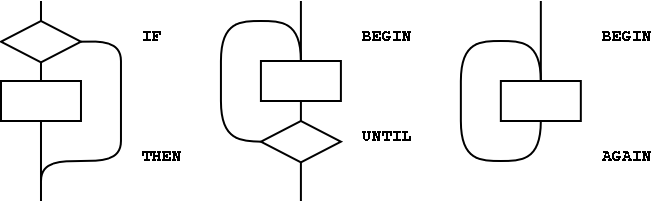
\includegraphics[bb=0 0 658 202,width=0.8\textwidth]{basic.png}}
	\caption{The basic control-flow patterns}
	\label{fig:basic}
  \end{center}
\end{figure}

In control flow every branch, or transfer of control, must terminate
at some destination. A natural implementation uses a stack to
remember the origin of forward branches and the destination of
backward branches. At a minimum, only the location of each origin or
destination must be indicated, although other implementation-dependent
information also may be maintained.

An origin is the location of the branch itself. A destination is
where control would continue if the branch were taken. A destination
is needed to resolve the branch address for each origin, and conversely,
if every control-flow path is completed no unused destinations can
remain.

With the addition of just three words (\word[tools]{AHEAD},
\word[tools]{CS-ROLL} and \word[tools]{CS-PICK}), the basic control-flow
words supply the primitives necessary to compile a variety of transportable
control structures. The abilities required are compilation of forward
and backward conditional and unconditional branches and compile-time
management of branch origins and destinations. \textbf{Table
\ref{table:control}} shows the desired behavior.

\begin{table}[ht]
  \begin{center}
	\caption{Compilation behavior of control-flow words}
	\label{table:control}
	\begin{tabular}{lccl}
	\hline\hline
	\multicolumn{4}{l}{at compile time,} \\
	word: & supplies: & resolves: & is used to: \\ \hline
	\word{IF}				& \emph{orig}	&				&
	mark origin of forward conditional branch \\
	\word{THEN}				&				& \emph{orig}	&
	resolve \word{IF} or \word[tools]{AHEAD} \\
	\word{BEGIN}			& \emph{dest}	&				&
	mark backward destination \\
	\word{AGAIN}			&				& \emph{dest}	&
	resolve with backward unconditional branch \\
	\word{UNTIL}			&				& \emph{dest}	&
	resolve with backward conditional branch \\
	\word[tools]{AHEAD}		& \emph{orig}	&				&
	mark origin of forward unconditional branch \\
	\word[tools]{CS-PICK}	&				&				&
	copy item on control-flow stack \\
	\word[tools]{CS-ROLL}	&				&				&
	reorder items on control-flow stack \\
	\hline\hline
	\end{tabular}
  \end{center}
\end{table}

The requirement that control-flow words are properly balanced by other
control-flow words makes reasonable the description of a compile-time
implementation-defined \emph{control-flow stack}. There is no
prescription as to how the control-flow stack is implemented, e.g.,
data stack, linked list, special array. Each element of the
control-flow stack mentioned above is the same size.

With these tools, the remaining basic control-structure elements,
shown in \textbf{figure \ref{fig:additional}}, can be defined. The
stack notation used here for immediate words is ( \emph{compilation
/ execution} ).

\begin{quote}\ttfamily
  \begin{tabbing}
	\tab \= \hspace{10em} \= \kill
	\+ \word{:} \word{WHILE}~ \word{p} dest -- orig dest / flag -- ) \\
		\word{bs} conditional exit from loops \\
		\word{POSTPONE} \word{IF}		\> \word{bs} conditional forward brach \\
	\-	1 \word[tools]{CS-ROLL}			\> \word{bs} keep dest on top \\
	\word{;} \word{IMMEDIATE} \\[2\parskip]

	\+	\word{:} \word{REPEAT}~ \word{p} orig dest -- / -- ) \\
		\word{bs} resolve a single WHILE and return to BEGIN \\
		\word{POSTPONE} \word{AGAIN}	\> \word{bs} uncond. backward branch to dest \\
	\-	\word{POSTPONE} \word{THEN}		\> \word{bs} resolve forward branch from orig \\
	\word{;} \word{IMMEDIATE} \\[2\parskip]

	\+ \word{:} \word{ELSE}~ \word{p} orig1 -- orig2 / -- ) \\
		\word{bs} resolve IF supplying alternate execution \\
		\word{POSTPONE} \word[tools]{AHEAD}	\> \word{bs} unconditional forward branch orig2 \\
		1 \word[tools]{CS-ROLL}				\> \word{bs} put orig1 back on top \\
	\-	\word{POSTPONE} \word{THEN}			\> \word{bs} resolve forward branch from orig1 \\
	\word{;} \word{IMMEDIATE}
  \end{tabbing}
\end{quote}

\begin{figure}[ht]
  \begin{center}
	\fbox{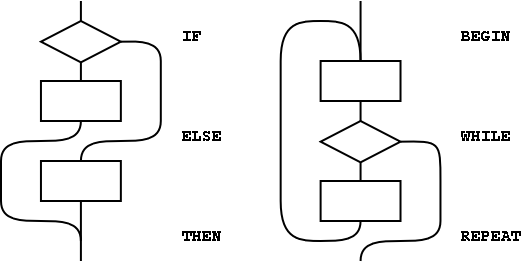
\includegraphics[bb=0 0 529 262,width=0.8\textwidth]{additional.png}}
	\caption{Additional basic control-flow patterns}
	\label{fig:additional}
  \end{center}
\end{figure}

Forth control flow provides a solution for well-known problems with
strictly structured programming.

The basic control structures can be supplemented, as shown in the
examples in \textbf{figure \ref{fig:extended}}, with additional
\word{WHILE}s in \word{BEGIN} {\ldots} \word{UNTIL} and \word{BEGIN}
{\ldots} \word{WHILE} {\ldots} \word{REPEAT} structures. However, for
each additional \word{WHILE} there must be a \word{THEN} at the end
of the structure. \word{THEN} completes the syntax with \word{WHILE}
and indicates where to continue execution when the \word{WHILE}
transfers control. The use of more than one additional \word{WHILE}
is possible but not common. Note that if the user finds this use of
\word{THEN} undesirable, an alias with a more likable name could be
defined.

Additional actions may be performed between the control flow word (the
\word{REPEAT} or \word{UNTIL}) and the \word{THEN} that matches the
additional \word{WHILE}. Further, if additional actions are desired
for normal termination and early termination, the alternative actions
may be separated by the ordinary Forth \word{ELSE}. The termination
actions are all specified after the body of the loop.

\begin{figure}[ht]
  \begin{center}
	\fbox{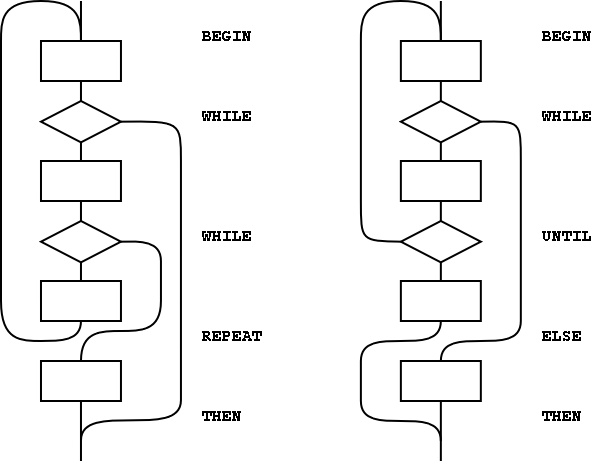
\includegraphics[bb=0 0 598 462, width=0.8\textwidth]{extended.png}}
	\caption{Extended control-flow patterns}
	\label{fig:extended}
  \end{center}
\end{figure}

Note that \word{REPEAT} creates an anomaly when matching the
\word{WHILE} with \word{ELSE} or \word{THEN}, most notably when
compared with the \word{BEGIN}{\ldots}\word{UNTIL} case. That is,
there will be one less \word{ELSE} or \word{THEN} than there are
\texttt{WHILE}s because \word{REPEAT} resolves one \word{THEN}. As
above, if the user finds this count mismatch undesirable, \word{REPEAT}
could be replaced in-line by its own definition.

Other loop-exit control-flow words, and even other loops, can be
defined. The only requirements are that the control-flow stack is
properly maintained and manipulated.

The simple implementation of the ANS Forth \word{CASE} structure
below is an example of control structure extension. Note the
maintenance of the data stack to prevent interference with the
possible control-flow stack usage.

\begin{quote}\ttfamily
  \begin{tabbing}
	\tab \= \hspace{10em} \= \kill
	0 \word{CONSTANT} \word{CASE} \word{IMMEDIATE}~ \word{p} init count of OFs ) \\[2\parskip]

	\+ \word{:} \word{OF}~ \word{p} \#of -- orig \#of+1 / x -- ) \\
		\word{1+}					\> \word{p} count OFs ) \\
		\word{toR}					\> \word{p} move off the stack in case the control-flow ) \\
									\> \word{p} stack is the data stack. ) \\
		\word{POSTPONE} \word{OVER}~ \word{POSTPONE} \word{=}~
								\word{p} copy and test case value) \\
		\word{POSTPONE} \word{IF}	\> \word{p} add orig to control flow stack ) \\
		\word{POSTPONE} \word{DROP}	\> \word{p} discards case value if = ) \\
	\-	\word{Rfrom}				\> \word{p} we can bring count back now ) \\
	\word{;} \word{IMMEDIATE} \\[2\parskip]

	\+ \word{:} \word{ENDOF}~ \word{p} orig1 \#of -- orig2 \#of ) \\
		\word{toR}					\> \word{p} move off the stack in case the control-flow ) \\
									\> \word{p} stack is the data stack. ) \\
		\word{POSTPONE} \word{ELSE} \\
	\-	\word{Rfrom}				\> \word{p} we can bring count back now ) \\
	\word{;} \word{IMMEDIATE} \\[2\parskip]

	\+ \word{:} \word{ENDCASE}~ \word{p} orig1..orign \#of -- ) \\
		\word{POSTPONE} \word{DROP}	\> \word{p} discard case value ) \\
		0 \word{qDO} \\
		\tab \word{POSTPONE} \word{THEN} \\
	\- \word{LOOP} \\
	\word{;} \word{IMMEDIATE}
  \end{tabbing}
\end{quote}


\paragraph{Return stack} ~ % A.3.2.3.3

The restrictions in section \xref[3.2.3.3 Return stack]{usage:returnstack}
are necessary if implementations are to be allowed to place loop
parameters on the return stack.

\subsubsection{Environmental queries} % A.3.2.6

The size in address units of various data types may be determined by
phrases such as \texttt{1} \word{CHARS}. Similarly, alignment may be
determined by phrases such as \texttt{1} \word{ALIGNED}.

The environmental queries are divided into two groups: those that
always produce the same value and those that might not. The former
groups include entries such as \texttt{MAX-N}. This information is
fixed by the hardware or by the design of the Forth system; a user
is guaranteed that asking the question once is sufficient.

The other group of queries are for things that may legitimately
change over time. For example an application might test for the
presence of the Double Number word set using an environment query.
If it is missing, the system could invoke a system-dependent process
to load the word set. The system is permitted to change
\word{ENVIRONMENTq}'s database so that subsequent queries about it
indicate that it is present.

Note that a query that returns an ``unknown'' response could produce
a ``known'' result on a subsequent query.


\subsection{The Forth dictionary} % A.3.3

A Standard Program may redefine a standard word with a non-standard
definition. The program is still Standard (since it can be built on
any Standard System), but the effect is to make the combined entity
(Standard System plus Standard Program) a non-standard system.

\subsubsection{Name space} % A.3.3.1

\setcounter{paragraph}{1}
\paragraph{Definition names} ~ % A.3.3.1.2

The language in this section is there to ensure the portability of
Standard Programs. If a program uses something outside the Standard
that it does not provide itself, there is no guarantee that another
implementation will have what the program needs to run. There is no
intent whatsoever to imply that all Forth programs will be somehow
lacking or inferior because they are not standard; some of the finest
jewels of the programmer's art will be non-standard. At the same time,
the committee is trying to ensure that a program labeled ``Standard''
will meet certain expectations, particularly with regard to portability.

In many system environments the input source is unable to supply
certain non-graphic characters due to external factors, such as the
use of those characters for flow control or editing. In addition,
when interpreting from a text file, the parsing function specifically
treats non-graphic characters like spaces; thus words received by the
text interpreter will not contain embedded non-graphic characters. To
allow implementations in such environments to call themselves Standard,
this minor restriction on Standard Programs is necessary.

A Standard System is allowed to permit the creation of definition
names containing non-graphic characters. Historically, such names
were used for keyboard editing functions and ``invisible'' words.

\subsubsection{Code space} % A.3.3.2

\subsubsection{Data space} % A.3.3.3

The words \word{numTIB}, \word{toIN}, \word{BASE}, \word[block]{BLK},
\word[block]{SCR}, \word{SOURCE}, \word{SOURCE-ID}, \word{STATE}, and
\word{TIB} contain information used by the Forth system in its
operation and may be of use to the application. Any assumption made
by the application about data available in the Forth system it did
not store other than the data just listed is an environmental
dependency.

There is no point in specifying (in the Standard) both what is and
what is not addressable. A Standard Program may NOT address:

\begin{itemize}
\item Directly into the data or return stacks;
\item Into a definition's data field if not stored by the application.
\end{itemize}

The read-only restrictions arise because some Forth systems run from
ROM and some share I/O buffers with other users or systems. Portable
programs cannot know which areas are affected, hence the general
restrictions.

\paragraph{Address alignment} ~ % A.3.3.3.1

Many processors have restrictions on the addresses that can be used
by memory access instructions. For example, on a Motorola 68000,
16-bit or 32-bit data can be accessed only at even addresses. Other
examples include RISC architectures where 16-bit data can be loaded
or stored only at even addresses and 32-bit data only at addresses
that are multiples of four.

An implementor of ANS Forth can handle these alignment restrictions
in one of two ways. Forth's memory access words (\word{@}, \word{!},
\word{+!}, etc.) could be implemented in terms of smaller-width access
instructions which have no alignment restrictions. For example, on a
68000 Forth with 16-bit cells, \word{@} could be implemented with two
68000 byte-fetch instructions and a reassembly of the bytes into a
16-bit cell. Although this conceals hardware restrictions from the
programmer, it is inefficient, and may have unintended side effects
in some hardware environments. An alternate implementation of ANS Forth
could define each memory-access word using the native instructions
that most closely match the word's function. On a 68000 Forth with
16-bit cells, \word{@} would use the 68000's 16-bit move instruction.
In this case, responsibility for giving \word{@} a correctly-aligned
address falls on the programmer. A portable ANS Forth program must
assume that alignment may be required and follow the requirements of
this section.

\paragraph{Contiguous regions} ~ % A.3.3.3.2

The data space of a Forth system comes in discontinuous regions! The
location of some regions is provided by the system, some by the
program. Data space is contiguous within regions, allowing address
arithmetic to generate valid addresses only within a single region.
A Standard Program cannot make any assumptions about the relative
placement of multiple regions in memory.

Section \ref{usage:contiguous} does prescribe conditions under which
contiguous regions of data space may be obtained. For example:
\begin{quote}\ttfamily
	\word{CREATE} TABLE \quad
	1 \word{C,} 2 \word{C,} \word{ALIGN} 1000 \word{,} 2000 \word{,}
\end{quote}
makes a table whose address is returned by \texttt{TABLE}. In
accessing this table,
\begin{quote}
  \begin{tabular}{ll}
	\texttt{TABLE} \word{C@}					& will return 1 \\
	\texttt{TABLE} \word{CHAR+} \word{C@}		& will return 2 \\
	\texttt{TABLE} \texttt{2} \word{CHARS} \word{+}
		\word{ALIGNED} \word{@}					& will return 1000 \\
	\texttt{TABLE} \texttt{2} \word{CHARS} \word{+}
		\word{ALIGNED} \word{CELL+} \word{@}	&  will return 2000. \\
  \end{tabular}
\end{quote}
Similarly,
\begin{quote}\ttfamily
	\word{CREATE} DATA \quad 1000 \word{ALLOT}
\end{quote}
makes an array 1000 address units in size. A more portable strategy
would define the array in application units, such as:
\begin{quote}\ttfamily
	500 \word{CONSTANT} NCELLS \\
	\word{CREATE} CELL-DATA NCELLS \word{CELLS} \word{ALLOT}
\end{quote}

This array can be indexed like this:
\begin{quote}\ttfamily
	\word{:} LOOK \quad
		NCELLS 0 \word{DO}
			CELL-DATA \word{I} \word{CELLS} \word{+} \word[tools]{q}
		\word{LOOP}
	\word{;}
\end{quote}


\setcounter{paragraph}{5}
\paragraph{Other transient regions} ~ % A.3.3.3.6

In many existing Forth systems, these areas are at \word{HERE} or
just beyond it, hence the many restrictions.

$(2*n)+2$ is the size of a character string containing the
unpunctuated binary representation of the maximum double number with
a leading minus sign and a trailing space.

Implementation note: Since the minimum value of \param{n} is 16, the
absolute minimum size of the pictured numeric output string is 34
characters. But if your implementation has a larger \param{n}, you must
also increase the size of the pictured numeric output string.

\subsection{The Forth text interpreter} % A.3.4

\subsubsection{Semantics} % A.3.4.3

The ``initiation semantics'' correspond to the code that is executed
upon entering a definition, analogous to the code executed by
\word{EXIT} upon leaving a definition. The ``run-time semantics''
correspond to code fragments, such as literals or branches, that are
compiled inside colon definitions by words with explicit compilation
semantics.

In a Forth cross-compiler, the execution semantics may be specified
to occur in the host system only, the target system only, or in both
systems. For example, it may be appropriate for words such as
\word{CELLS} to execute on the host system returning a value describing
the target, for colon definitions to execute only on the target, and
for \word{CONSTANT} and \word{VARIABLE} to have execution behaviors on
both systems. Details of cross-compiler behavior are beyond the scope
of this Standard.

\setcounter{paragraph}{1}
\paragraph{Interpretation semantics} ~ % A.3.4.3.2
\label{rat:interpret}

For a variety of reasons, this Standard does not define interpretation
semantics for every word. Examples of these words are \word{toR},
\word{.q}, \word{DO}, and \word{IF}. Nothing in this Standard precludes
an implementation from providing interpretation semantics for these
words, such as interactive control-flow words. However, a Standard
Program may not use them in interpretation state.

\subsubsection{Compilation} % A.3.4.5

Compiler recursion at the definition level consumes excessive
resources, especially to support locals. The Technical Committee
does not believe that the benefits justify the costs. Nesting
definitions is also not common practice and won't work on many
systems.

\section{Documentation requirements} % A.4 ==========================

\subsection{System documentation} % A.4.1

\subsection{Program documentation} % A.4.2

\section{Compliance and labeling} % A.5 =============================

\subsection{ANS Forth systems} % A.5.1

Section \ref{label:label} defines the criteria that a system must
meet in order to justify the label ``ANS Forth System''. Briefly,
the minimum requirement is that the system must ``implement'' the
Core word set. There are several ways in which this requirement may
be met. The most obvious is that all Core words may be in a pre-compiled
kernel. This is not the only way of satisfying the requirement,
however. For example, some words may be provided in source blocks or
files with instructions explaining how to add them to the system if
they are needed. So long as the words are provided in such a way that
the user can obtain access to them with a clear and straightforward
procedure, they may be considered to be present.

A Forth cross-compiler has many characteristics in common with an ANS
Forth System, in that both use similar compiling tools to process a
program. However, in order to fully specify an ANS Forth cross compiler
it would be necessary to address complex issues dealing with compilation
and execution semantics in both host and target environments as well as
ROMability issues. The level of effort to do this properly has proved to
be impractical at this time. As a result, although it may be possible
for a Forth cross-compiler to correctly prepare an ANS Forth program
for execution in a target environment, it is inappropriate for a
cross-compiler to be labeled an ANS Forth System.

\subsection{ANS Forth programs} % A.5.2

\setcounter{subsubsection}{1}
\subsubsection{Program labeling} % A.5.2.2

Declaring an environmental dependency should not be considered
undesirable, merely an acknowledgment that the author has taken
advantage of some assumed architecture. For example, most computers
in common use are based on two's complement binary arithmetic. By
acknowledging an environmental dependency on this architecture,
a programmer becomes entitled to use the number \texttt{-1} to
represent all bits set without significantly restricting the
portability of the program.

Because all programs require space for data and instructions, and
time to execute those instructions, they depend on the presence of
an environment providing those resources. It is impossible to predict
how little of some of these resources (e.g. stack space) might be
necessary to perform some task, so this Standard does not do so.

On the other hand, as a program requires increasing levels of
resources, there will probably be sucessively fewer systems on
which it will execute sucessfully. An algorithm requiring an array
of $10^9$ cells might run on fewer computers than one requiring
only $10^3$.

Since there is also no way of knowing what minimum level of resources
will be implemented in a system useful for at least some tasks, any
program performing real work labeled simply an ``ANS Forth Program''
is unlikely to be labeled correctly.


\section{Glossary} % A.6 ============================================

In this and following sections we present rationales for the handling
of specific words: why we included them, why we placed them in certain
word sets, or why we specified their names or meaning as we did.

Words in this section are organized by word set, retaining their index
numbers for easy cross-referencing to the glossary.

Historically, many Forth systems have been written in Forth. Many of
the words in Forth originally had as their primary purpose support of
the Forth system itself. For example, \word{WORD} and \word{FIND} are
often used as the principle instruments of the Forth text interpreter,
and \word{CREATE} in many systems is the primitive for building
dictionary entries. In defining words such as these in a standard way,
we have endeavored not to do so in such a way as to preclude their use
by implementors. One of the features of Forth that has endeared it to
its users is that the same tools that are used to implement the system
are available to the application programmer --- a result of this
approach is the compactness and efficiency that characterizes most
Forth implementations.

\Ifanswerfiles{
	\ifinlinebody
		~\par
		In the \emph{rationale} (r) version of the document,
		the rationale text for each of the word sets are given  here.
		While the rationale for the individual words are given in the
		word's definition.
	\fi
	\ifinlineintro
		~\par
		In the \emph{wordlist} (w) version of the document,
		the rationale text for each of the word sets are given in the
		main text. It is indented and the label ``(Rationale)'' is
		included in the section heading.
		The rationale for the individual words are given here.
		\par~\par
	\fi
	\chapter{Glossary} % 6

\section{Core words} % 6.1
\wordlist{core}

\begin{worddef}{0010}{!}[store]
\item \stack{x a-addr}{}

	Store \param{x} at \param{a-addr}.

	\see \xref[3.3.3.1 Address alignment]{usage:aaddr}.

	\begin{defer}
	\testing*
		See \rref{core:,}{,}
	\end{defer}
\end{worddef}


\begin{worddef}[num]{0030}{\num}[number-sign]
\item \stack{ud_1}{ud_2}

	Divide \param{ud_1} by the number in \word{BASE} giving the
	quotient \param{ud_2} and the remainder \param{n}. (\param{n} is
	the least significant digit of \param{ud_1}.) Convert \param{n}
	to external form and add the resulting character to the beginning
	of the pictured numeric output string. An ambiguous condition
	exists if \word{num} executes outside of a \word{num-end}
	\word{num-start} delimited number conversion.

\see \wref{core:num-end}{\num>},
	\wref{core:numS}{\num{}S},
	\wref{core:num-start}{<\num}.

	\begin{defer}
	\testing
		\word{:} GP3  \word{num-start} 1 0 \word{num} \word{num} \word{num-end} \word{Sq} 01" S= \word{;} \\
		\{ GP3 -> <TRUE> \}
	\end{defer}
\end{worddef}


\begin{worddef}[num-end]{0040}{\num>}[number-sign-greater]
\item \stack{xd}{c-addr u}

	Drop \param{xd}. Make the pictured numeric output string
	available as a character string. \param{c-addr} and \param{u}
	specify the resulting character string. A program may replace
	characters within the string.

\see \wref{core:num}{\num},
	\wref{core:numS}{\num{}S},
	\wref{core:num-start}{<\num}.

	\begin{defer}
	\testing*
		See \rref{core:num}{\num},
			\rref{core:numS}{\num{}S},
			\rref{core:HOLD}{HOLD} and
			\rref{core:SIGN}{SIGN}.
	\end{defer}
\end{worddef}


\begin{worddef}[numS]{0050}{\num{}S}[number-sign-s]
\item \stack{ud_1}{ud_2}

	Convert one digit of \param{ud_1} according to the rule for
	\word{num}. Continue conversion until the quotient is zero.
	\param{ud_2} is zero. An ambiguous condition exists if
	\word{numS} executes outside of a \word{num-start} \word{num-end}
	delimited number conversion.

\see \wref{core:num}{\num},
	\wref{core:num-end}{\num>},
	\wref{core:num-start}{<\num}.

	\begin{defer}
	\testing
		\word{:} GP4  \word{num-start} 1 0 \word{numS} \word{num-end} \word{Sq} 1" S= \word{;} \\
		\{ GP4 -> <TRUE> \}

		\word{:} GP5 \\
		\tab \word{BASE} \word{@} <TRUE> \\
		\tab MAX-BASE \word{1+} 2 \word{DO}		\tab[2] \word{bs} FOR EACH POSSIBLE BASE \\
		\tab[2] \word{I} \word{BASE} \word{!}	\tab[4.7] \word{bs} TBD: ASSUMES BASE WORKS \\
		\tab[3] \word{I} 0 \word{num-start} \word{numS} \word{num-end} \word{Sq} 10" S= \word{AND} \\
		\tab    \word{LOOP} \\
		\tab    \word{SWAP} \word{BASE} \word{!} \word{;} \\
		\{ GP5 -> <TRUE> \}

		\word{:} GP6 \\
		\tab	\word{BASE} \word{@} \word{toR}  2 \word{BASE} \word{!} \\
		\tab	MAX-UINT MAX-UINT \word{num-start} \word{numS} \word{num-end}	\tab[2]	  \word{bs} MAXIMUM UD TO BINARY \\
		\tab	\word{Rfrom} \word{BASE} \word{!}								\tab[10.9] \word{bs} S: C-ADDR U \\
		\tab	\word{DUP} \#BITS-UD \word{=} \word{SWAP} \\
		\tab	0 \word{DO}														\tab[13.4]  \word{bs} S: C-ADDR FLAG \\
		\tab[2]		\word{OVER} \word{C@} \word{[CHAR]} 1 \word{=} \word{AND}	\tab[2.5] \word{bs} ALL ONES \\
		\tab[2]		\word{toR} \word{CHAR+} \word{Rfrom} \\
		\tab	\word{LOOP} \word{SWAP} \word{DROP} \word{;} \\
		\{ GP6 -> <TRUE> \}

		\word{:} GP7 \\
		\tab	\word{BASE} \word{@} \word{toR}		MAX-BASE \word{BASE} \word{!} \\
		\tab	<TRUE> \\
		\tab	A 0 \word{DO} \\
		\tab[2]		\word{I} 0 \word{num-start} \word{numS} \word{num-end} \\
		\tab[2]		1 \word{=} \word{SWAP} \word{C@} \word{I} 30 \word{+} \word{=} \word{AND} \word{AND} \\
		\tab	\word{LOOP} \\
		\tab	MAX-BASE A \word{DO} \\
		\tab[2]		\word{I} 0 \word{num-start} \word{numS} \word{num-end} \\
		\tab[2]		1 \word{=} \word{SWAP} \word{C@} 41 \word{I} A \word{-} \word{+} \word{=} \word{AND} \word{AND} \\
		\tab	\word{LOOP} \\
		\tab	\word{Rfrom} \word{BASE} \word{!} \word{;} \\
		\{ GP7 -> <TRUE> \}
	\end{defer}
\end{worddef}


\begin{worddef}{0070}{'}[tick]
\item \stack{"<spaces>name"}{xt}

	Skip leading space delimiters. Parse \param{name} delimited by
	a space. Find \param{name} and return \param{xt}, the execution
	token for \param{name}. An ambiguous condition exists if
	\param{name} is not found. When interpreting,
	\texttt{' xyz EXECUTE} is equivalent to \texttt{xyz}.

\see \xref[3.4 The Forth text interpreter]{usage:interpret},
	\xref[3.4.1 Parsing]{usage:parsing},
	\rref{core:POSTPONE}{POSTPONE},
	\rref{core:[']}{[']},
	\xref[D.6.7 Immediacy]{diff:immediate}.

	\begin{defer}
	\rationale % A.6.1.0070 '
		Typical use: {\ldots} \word{'} \param{name}.

		Many Forth systems use a state-smart tick. Many do not.
		ANS Forth follows the usage of Forth 83.

	\see \xref[A.3.4.3..2 Interpretation semantics]{rat:interpret},
		\rref{core:FIND}{FIND}.

	\testing
		\{ \word{:} GT1 123 \word{;} -> \} \\
		\{ \word{'} GT1 \word{EXECUTE} -> 123 \}
	\end{defer}
\end{worddef}


\begin{worddef}[p]{0080}{(}[paren]
\compile
	Perform the execution semantics given below.

\execute
	\stack{"ccc<paren>"}{}

	Parse \param{ccc} delimited by \word{p} (right parenthesis).
	\word{p} is an immediate word.

	The number of characters in \param{ccc} may be zero to the
	number of characters in the parse area.

\see \xref[3.4.1 Parsing]{usage:parsing},
	\xref[11.6.1.0080 (]{file:p}.

	\begin{defer}
	\rationale % A.6.1.0080 (
		Typical use: {\ldots} \word{p} \param{ccc}\texttt{)} {\ldots}

	\testing* None.
	\end{defer}
\end{worddef}


\begin{worddef}{0090}{*}[star]
\item \stack{n_1|u_1 n_2|u_2}{n_3|u_3}

	Multiply \param{n_1|u_1} by \param{n_2|u_2} giving the product
	\param{n_3|u_3}.

	\begin{defer}
	\testing
		\{  0  0 \word{*} ->  0 \} \tab[4] \word{bs} TEST IDENTITIE{\bs}S \\
		\{  0  1 \word{*} ->  0 \} \\
		\{  1  0 \word{*} ->  0 \} \\
		\{  1  2 \word{*} ->  2 \} \\
		\{  2  1 \word{*} ->  2 \} \\
		\{  3  3 \word{*} ->  9 \} \\
		\{ -3  3 \word{*} -> -9 \} \\
		\{  3 -3 \word{*} -> -9 \} \\
		\{ -3 -3 \word{*} ->  9 \}

		\{ MID-UINT+1 1 \word{RSHIFT} 2 \word{*} -> MID-UINT+1 \} \\
		\{ MID-UINT+1 2 \word{RSHIFT} 4 \word{*} -> MID-UINT+1 \} \\
		\{ MID-UINT+1 1 \word{RSHIFT} MID-UINT+1 \word{OR} 2 \word{*} -> MID-UINT+1 \} \\
	\end{defer}
\end{worddef}


\begin{worddef}{0100}{*/}[star-slash]
\item \stack{n_1 n_2 n_3}{n_4}

	Multiply \param{n_1} by \param{n_2} producing the intermediate
	double-cell result $d$. Divide $d$ by \param{n_3} giving the
	single-cell quotient \param{n_4}. An ambiguous condition exists
	if \param{n_3} is zero or if the quotient \param{n_4} lies
	outside the range of a signed number. If $d$ and \param{n_3}
	differ in sign, the implementation-defined result returned will
	be the same as that returned by either the phrase
	\word{toR} \word{M*} \word{Rfrom} \word{FM/MOD} \word{SWAP} \word{DROP}
	or the phrase
	\word{toR} \word{M*} \word{Rfrom} \word{SM/REM} \word{SWAP} \word{DROP}.

\see \xref[3.2.2.1 Integer division]{usage:div}.

	\begin{defer}
	\testing
		IFFLOORED \tab	\word{:} T*/ T*/MOD \word{SWAP} \word{DROP} \word{;} \\
		IFSYM \tab[2.6]	\word{:} T*/ T*/MOD \word{SWAP} \word{DROP} \word{;}

		\{       0 2       1 \word{*/} ->       0 2       1 T*/ \} \\
		\{       1 2       1 \word{*/} ->       1 2       1 T*/ \} \\
		\{       2 2       1 \word{*/} ->       2 2       1 T*/ \} \\
		\{      -1 2       1 \word{*/} ->      -1 2       1 T*/ \} \\
		\{      -2 2       1 \word{*/} ->      -2 2       1 T*/ \} \\
		\{       0 2      -1 \word{*/} ->       0 2      -1 T*/ \} \\
		\{       1 2      -1 \word{*/} ->       1 2      -1 T*/ \} \\
		\{       2 2      -1 \word{*/} ->       2 2      -1 T*/ \} \\
		\{      -1 2      -1 \word{*/} ->      -1 2      -1 T*/ \} \\
		\{      -2 2      -1 \word{*/} ->      -2 2      -1 T*/ \} \\
		\{       2 2       2 \word{*/} ->       2 2       2 T*/ \} \\
		\{      -1 2      -1 \word{*/} ->      -1 2      -1 T*/ \} \\
		\{      -2 2      -2 \word{*/} ->      -2 2      -2 T*/ \} \\
		\{       7 2       3 \word{*/} ->       7 2       3 T*/ \} \\
		\{       7 2      -3 \word{*/} ->       7 2      -3 T*/ \} \\
		\{      -7 2       3 \word{*/} ->      -7 2       3 T*/ \} \\
		\{      -7 2      -3 \word{*/} ->      -7 2      -3 T*/ \} \\
		\{ MAX-INT 2 MAX-INT \word{*/} -> MAX-INT 2 MAX-INT T*/ \} \\
		\{ MIN-INT 2 MIN-INT \word{*/} -> MIN-INT 2 MIN-INT T*/ \}
	\end{defer}
\end{worddef}


\begin{worddef}{0110}{*/MOD}[star-slash-mod]
\item \stack{n_1 n_2 n_3}{n_4 n_5}

	Multiply \param{n_1} by \param{n_2} producing the intermediate
	double-cell result $d$. Divide $d$ by \param{n_3} producing the
	single-cell remainder \param{n_4} and the single-cell quotient
	\param{n_5}. An ambiguous condition exists if \param{n_3} is
	zero, or if the quotient \param{n_5} lies outside the range of a
	single-cell signed integer. If $d$ and \param{n_3} differ in
	sign, the implementation-defined result returned will be the
	same as that returned by either the phrase
	\word{toR} \word{M*} \word{Rfrom} \word{FM/MOD} or the phrase
	\word{toR} \word{M*} \word{Rfrom} \word{SM/REM}.

\see \xref[3.2.2.1 Integer division]{usage:div}.

	\begin{defer}
	\testing
		IFFLOORED \tab	\word{:} T*/MOD \word{toR} \word{M*} \word{Rfrom} \word{FM/MOD} \word{;} \\
		IFSYM \tab[2.6]	\word{:} T*/MOD \word{toR} \word{M*} \word{Rfrom} \word{SM/REM} \word{;}

		\{       0 2       1 \word{*/MOD} ->       0 2       1 T*/MOD \} \\
		\{       1 2       1 \word{*/MOD} ->       1 2       1 T*/MOD \} \\
		\{       2 2       1 \word{*/MOD} ->       2 2       1 T*/MOD \} \\
		\{      -1 2       1 \word{*/MOD} ->      -1 2       1 T*/MOD \} \\
		\{      -2 2       1 \word{*/MOD} ->      -2 2       1 T*/MOD \} \\
		\{       0 2      -1 \word{*/MOD} ->       0 2      -1 T*/MOD \} \\
		\{       1 2      -1 \word{*/MOD} ->       1 2      -1 T*/MOD \} \\
		\{       2 2      -1 \word{*/MOD} ->       2 2      -1 T*/MOD \} \\
		\{      -1 2      -1 \word{*/MOD} ->      -1 2      -1 T*/MOD \} \\
		\{      -2 2      -1 \word{*/MOD} ->      -2 2      -1 T*/MOD \} \\
		\{       2 2       2 \word{*/MOD} ->       2 2       2 T*/MOD \} \\
		\{      -1 2      -1 \word{*/MOD} ->      -1 2      -1 T*/MOD \} \\
		\{      -2 2      -2 \word{*/MOD} ->      -2 2      -2 T*/MOD \} \\
		\{       7 2       3 \word{*/MOD} ->       7 2       3 T*/MOD \} \\
		\{       7 2      -3 \word{*/MOD} ->       7 2      -3 T*/MOD \} \\
		\{      -7 2       3 \word{*/MOD} ->      -7 2       3 T*/MOD \} \\
		\{      -7 2      -3 \word{*/MOD} ->      -7 2      -3 T*/MOD \} \\
		\{ MAX-INT 2 MAX-INT \word{*/MOD} -> MAX-INT 2 MAX-INT T*/MOD \} \\
		\{ MIN-INT 2 MIN-INT \word{*/MOD} -> MIN-INT 2 MIN-INT T*/MOD \} \\
	\end{defer}
\end{worddef}


\begin{worddef}{0120}{+}[plus]
\item \stack{n_1|u_1 n_2|u_2}{n_3|u_3}

	Add \param{n_2|u_2} to \param{n_1|u_1}, giving the sum
	\param{n_3|u_3}.

\see \xref[3.3.3.1 Address alignment]{usage:aaddr}.

	\begin{defer}
	\testing
		\{        0  5 \word{+} ->          5 \} \\
		\{        5  0 \word{+} ->          5 \} \\
		\{        0 -5 \word{+} ->         -5 \} \\
		\{       -5  0 \word{+} ->         -5 \} \\
		\{        1  2 \word{+} ->          3 \} \\
		\{        1 -2 \word{+} ->         -1 \} \\
		\{       -1  2 \word{+} ->          1 \} \\
		\{       -1 -2 \word{+} ->         -3 \} \\
		\{       -1  1 \word{+} ->          0 \} \\
		\{ MID-UINT  1 \word{+} -> MID-UINT+1 \}
	\end{defer}
\end{worddef}


\begin{worddef}{0130}{+!}[plus-store]
\item \stack{n|u a-addr}{}

	Add \param{n|u} to the single-cell number at \param{a-addr}.

\see \xref[3.3.3.1 Address alignment]{usage:aaddr}.

	\begin{defer}
	\testing
		\{  0 1ST \word{!}  -> \} \\
		\{  1 1ST \word{+!} -> \} \\
		\{    1ST \word{@}  -> 1 \} \\
		\{ -1 1ST \word{+!} 1ST \word{@} -> 0 \}
	\end{defer}
\end{worddef}


\begin{worddef}{0140}{+LOOP}[plus-loop]
\interpret
	Interpretation semantics for this word are undefined.

\compile
	\stack[C]{do-sys}{}

	Append the run-time semantics given below to the current
	definition. Resolve the destination of all unresolved
	occurrences of \word{LEAVE} between the location given
	by \param{do-sys} and the next location for a transfer of
	control, to execute the words following \word{+LOOP}.

\runtime
	\stack{n}{}
	\stack[R]{loop-sys_1}{|loop-sys_2}

	An ambiguous condition exists if the loop control parameters
	are unavailable. Add \param{n} to the loop index. If the loop
	index did not cross the boundary between the loop limit minus
	one and the loop limit, continue execution at the beginning
	of the loop. Otherwise, discard the current loop control
	parameters and continue execution immediately following the
	loop.

\see \wref{core:DO}{DO},
	\wref{core:I}{I},
	\wref{core:LEAVE}{LEAVE}.

	\begin{defer}
	\rationale % A.6.1.0140 +LOOP
		Typical use:
			\word{:} \texttt{X} ~{\ldots} limit first \word{DO}
				{\ldots} step \word{+LOOP}
			\word{;}

	\testing
		\{ \word{:} GD2 \word{DO} \word{I} -1 \word{+LOOP} \word{;} -> \} \\
		\{        1          4 GD2 -> 4 3 2 1 \} \\
		\{       -1          2 GD2 -> 2 1 0 -1 \} \\
		\{ MID-UINT MID-UINT+1 GD2 -> MID-UINT+1 MID-UINT \}
	\end{defer}
\end{worddef}


\begin{worddef}{0150}{,}[comma]
\item \stack{x}{}

	Reserve one cell of data space and store \param{x} in the cell.
	If the data-space pointer is aligned when \word{,} begins
	execution, it will remain aligned when \word{,} finishes
	execution. An ambiguous condition exists if the data-space
	pointer is not aligned prior to execution of \word{,}.

\see \xref[3.3.3 Data space]{usage:dataspace},
	\xref[3.3.3.1 Address alignment]{usage:aaddr}.

	\begin{defer}
	\rationale % A.6.1.0150 ,
		The use of \word{,} (comma) for compiling execution tokens is
		not portable.

		See: \wref{core:COMPILE,}{COMPILE,}.

	\testing
		\word{HERE} 1 \word{,} \\
		\word{HERE} 2 \word{,} \\
		\word{CONSTANT} 2ND \\
		\word{CONSTANT} 1ST

		\{ 1ST 2ND \word{Uless} -> <TRUE> \}	\tab \word{bs} HERE MUST GROW WITH ALLOT \\
		\{ 1ST \word{CELL+} -> 2ND \}			\tab[2.6] \word{bs} {\ldots} BY ONE CELL \\
		\{ 1ST 1 \word{CELLS} \word{+} -> 2ND \} \\
		\{ 1ST \word{@} 2ND \word{@} -> 1 2 \} \\
		\{ 5 1ST \word{!} -> \} \\
		\{ 1ST \word{@} 2ND \word{@} -> 5 2 \} \\
		\{ 6 2ND \word{!} -> \} \\
		\{ 1ST \word{@} 2ND \word{@} -> 5 6 \} \\
		\{ 1ST \word{2@} -> 6 5 \} \\
		\{ 2 1 1ST \word{2!} -> \} \\
		\{ 1ST \word{2@} -> 2 1 \} \\
		\{ 1S 1ST \word{!}  1ST \word{@} -> 1S \} \tab \word{bs} CAN STORE CELL-WIDE VALUE
	\end{defer}
\end{worddef}


\begin{worddef}{0160}{-}[minus]
\item \stack{n_1|u_1 n_2|u_2}{n_3|u_3}

	Subtract \param{n_2|u_2} from \param{n_1|u_1}, giving the
	difference \param{n_3|u_3}.

\see \xref[3.3.3.1 Address alignment]{usage:aaddr}.

	\begin{defer}
	\testing
		\{          0  5 \word{-} ->       -5 \} \\
		\{          5  0 \word{-} ->        5 \} \\
		\{          0 -5 \word{-} ->        5 \} \\
		\{         -5  0 \word{-} ->       -5 \} \\
		\{          1  2 \word{-} ->       -1 \} \\
		\{          1 -2 \word{-} ->        3 \} \\
		\{         -1  2 \word{-} ->       -3 \} \\
		\{         -1 -2 \word{-} ->        1 \} \\
		\{          0  1 \word{-} ->       -1 \} \\
		\{ MID-UINT+1  1 \word{-} -> MID-UINT \}
	\end{defer}
\end{worddef}


\begin{worddef}[d]{0180}{.{}}[dot]
\item \stack{n}{}

	Display \param{n} in free field format.

\see \xref[3.2.1.2 Digit conversion]{usage:digits},
	\xref[3.2.1.3 Free-field number display]{usage:dot}.

	\begin{defer}
	\testing*
	\see \rref{core:EMIT}{EMIT}.
	\end{defer}
\end{worddef}


\begin{worddef}[.q]{0190}{."}[dot-quote]
\interpret
	Interpretation semantics for this word are undefined.

\compile
	\stack{"ccc<quote>"}{}

	Parse \param{ccc} delimited by \texttt{"} (double-quote).
	Append the run-time semantics given below to the current
	definition.

\runtime
	\stack{}{}

	Display \param{ccc}.

\see \xref[3.4.1 Parsing]{usage:parsing},
	\wref{core:.p}{.(}.

	\begin{defer}
	\rationale % A.6.1.0190 ."
		Typical use:
			\word{:} \texttt{X} {\ldots}
				\word{.q} \emph{ccc}\texttt{"} {\ldots}
			\word{;}

		An implementation may define interpretation semantics for
		\word{.q} if desired. In one plausible implementation,
		interpreting \word{.q} would display the delimited message.
		In another plausible implementation, interpreting \word{.q}
		would compile code to display the message later. In still
		another plausible implementation, interpreting \word{.q} would
		be treated as an exception. Given this variation a Standard
		Program may not use \word{.q} while interpreting. Similarly,
		a Standard Program may not compile \word{POSTPONE} \word{.q}
		inside a new word, and then use that word while interpreting.

	\testing*
		See \rref{core:EMIT}{EMIT}.
	\end{defer}
\end{worddef}


\begin{worddef}{0230}{/}[slash]
\item \stack{n_1 n_2}{n_3}

	Divide \param{n_1} by \param{n_2}, giving the single-cell quotient
	\param{n_3}. An ambiguous condition exists if \param{n_2} is zero.
	If \param{n_1} and \param{n_2} differ in sign, the
	implementation-defined result returned will be the same as that
	returned by either the phrase
	\word{toR} \word{StoD} \word{Rfrom} \word{FM/MOD} \word{SWAP} \word{DROP}
	or the phrase
	\word{toR} \word{StoD} \word{Rfrom} \word{SM/REM} \word{SWAP} \word{DROP}.

\see \xref[3.2.2.1 Integer division]{usage:div}.

	\begin{defer}
	\testing
		IFFLOORED \tab	\word{:} T/ T/MOD \word{SWAP} \word{DROP} \word{;} \\
		IFSYM \tab[2.6] \word{:} T/ T/MOD \word{SWAP} \word{DROP} \word{;}

		\{       0       1 \word{/} ->       0       1 T/ \} \\
		\{       1       1 \word{/} ->       1       1 T/ \} \\
		\{       2       1 \word{/} ->       2       1 T/ \} \\
		\{      -1       1 \word{/} ->      -1       1 T/ \} \\
		\{      -2       1 \word{/} ->      -2       1 T/ \} \\
		\{       0      -1 \word{/} ->       0      -1 T/ \} \\
		\{       1      -1 \word{/} ->       1      -1 T/ \} \\
		\{       2      -1 \word{/} ->       2      -1 T/ \} \\
		\{      -1      -1 \word{/} ->      -1      -1 T/ \} \\
		\{      -2      -1 \word{/} ->      -2      -1 T/ \} \\
		\{       2       2 \word{/} ->       2       2 T/ \} \\
		\{      -1      -1 \word{/} ->      -1      -1 T/ \} \\
		\{      -2      -2 \word{/} ->      -2      -2 T/ \} \\
		\{       7       3 \word{/} ->       7       3 T/ \} \\
		\{       7      -3 \word{/} ->       7      -3 T/ \} \\
		\{      -7       3 \word{/} ->      -7       3 T/ \} \\
		\{      -7      -3 \word{/} ->      -7      -3 T/ \} \\
		\{ MAX-INT       1 \word{/} -> MAX-INT       1 T/ \} \\
		\{ MIN-INT       1 \word{/} -> MIN-INT       1 T/ \} \\
		\{ MAX-INT MAX-INT \word{/} -> MAX-INT MAX-INT T/ \} \\
		\{ MIN-INT MIN-INT \word{/} -> MIN-INT MIN-INT T/ \}
	\end{defer}
\end{worddef}


\begin{worddef}{0240}{/MOD}[slash-mod]
\item \stack{n_1 n_2}{n_3 n_4}

	Divide \param{n_1} by \param{n_2}, giving the single-cell remainder
	\param{n_3} and the single-cell quotient \param{n_4}. An ambiguous
	condition exists if \param{n_2} is zero. If \param{n_1} and
	\param{n_2} differ in sign, the implementation-defined result
	returned will be the same as that returned by either the phrase
	\word{toR} \word{StoD} \word{Rfrom} \word{FM/MOD}
	or the phrase
	\word{toR} \word{StoD} \word{Rfrom} \word{SM/REM}.

\see \xref[3.2.2.1 Integer division]{usage:div}.

	\begin{defer}
	\testing
		IFFLOORED \tab  \word{:} T/MOD  \word{toR} \word{StoD} \word{Rfrom} \word{FM/MOD} \word{;} \\
		IFSYM \tab[2.6] \word{:} T/MOD  \word{toR} \word{StoD} \word{Rfrom} \word{SM/REM} \word{;}

		\{       0       1 \word{/MOD} ->       0       1 T/MOD \} \\
		\{       1       1 \word{/MOD} ->       1       1 T/MOD \} \\
		\{       2       1 \word{/MOD} ->       2       1 T/MOD \} \\
		\{      -1       1 \word{/MOD} ->      -1       1 T/MOD \} \\
		\{      -2       1 \word{/MOD} ->      -2       1 T/MOD \} \\
		\{       0      -1 \word{/MOD} ->       0      -1 T/MOD \} \\
		\{       1      -1 \word{/MOD} ->       1      -1 T/MOD \} \\
		\{       2      -1 \word{/MOD} ->       2      -1 T/MOD \} \\
		\{      -1      -1 \word{/MOD} ->      -1      -1 T/MOD \} \\
		\{      -2      -1 \word{/MOD} ->      -2      -1 T/MOD \} \\
		\{       2       2 \word{/MOD} ->       2       2 T/MOD \} \\
		\{      -1      -1 \word{/MOD} ->      -1      -1 T/MOD \} \\
		\{      -2      -2 \word{/MOD} ->      -2      -2 T/MOD \} \\
		\{       7       3 \word{/MOD} ->       7       3 T/MOD \} \\
		\{       7      -3 \word{/MOD} ->       7      -3 T/MOD \} \\
		\{      -7       3 \word{/MOD} ->      -7       3 T/MOD \} \\
		\{      -7      -3 \word{/MOD} ->      -7      -3 T/MOD \} \\
		\{ MAX-INT       1 \word{/MOD} -> MAX-INT       1 T/MOD \} \\
		\{ MIN-INT       1 \word{/MOD} -> MIN-INT       1 T/MOD \} \\
		\{ MAX-INT MAX-INT \word{/MOD} -> MAX-INT MAX-INT T/MOD \} \\
		\{ MIN-INT MIN-INT \word{/MOD} -> MIN-INT MIN-INT T/MOD \}
	\end{defer}
\end{worddef}


\begin{worddef}[0less]{0250}{0<}[zero-less]
\item \stack{n}{flag}

	\param{flag} is true if and only if \param{n} is less than zero.

	\begin{defer}
	\testing
		\{       0 \word{0less} -> <FALSE> \} \\
		\{      -1 \word{0less} -> <TRUE>  \} \\
		\{ MIN-INT \word{0less} -> <TRUE>  \} \\
		\{       1 \word{0less} -> <FALSE> \} \\
		\{ MAX-INT \word{0less} -> <FALSE> \}
	\end{defer}
\end{worddef}


\begin{worddef}{0270}{0=}[zero-equals]
\item \stack{x}{flag}

	\param{flag} is true if and only if \param{x} is equal to zero.

	\begin{defer}
	\testing
		\{  0 \word{0=} -> <TRUE>  \} \\
		\{  1 \word{0=} -> <FALSE> \} \\
		\{  2 \word{0=} -> <FALSE> \} \\
		\{ -1 \word{0=} -> <FALSE> \} \\
		\{ MAX-UINT \word{0=} -> <FALSE> \} \\
		\{ MIN-INT  \word{0=} -> <FALSE> \} \\
		\{ MAX-INT  \word{0=} -> <FALSE> \}
	\end{defer}
\end{worddef}


\begin{worddef}{0290}{1+}[one-plus]
\item \stack{n_1|u_1}{n_2|u_2}

	Add one (1) to \param{n_1|u_1} giving the sum
	\param{n_2|u_2}.

	\begin{defer}
	\testing
		\{        0 \word{1+} ->          1 \} \\
		\{       -1 \word{1+} ->          0 \} \\
		\{        1 \word{1+} ->          2 \} \\
		\{ MID-UINT \word{1+} -> MID-UINT+1 \}
	\end{defer}
\end{worddef}


\begin{worddef}{0300}{1-}[one-minus]
\item \stack{n_1|u_1}{n_2|u_2}

	Subtract one (1) from \param{n_1|u_1} giving the difference
	\param{n_2|u_2}.

	\begin{defer}
	\testing
		\{          2 \word{1-} ->        1 \} \\
		\{          1 \word{1-} ->        0 \} \\
		\{          0 \word{1-} ->       -1 \} \\
		\{ MID-UINT+1 \word{1-} -> MID-UINT \}
	\end{defer}
\end{worddef}


\begin{worddef}{0310}{2!}[two-store]
\item \stack{x_1 x_2 a-addr}{}

	Store the cell pair \param{x_1 x_2} at \param{a-addr}, with
	\param{x_2} at \param{a-addr} and \param{x_1} at the next
	consecutive cell. It is equivalent to the sequence
	\word{SWAP} \word{OVER} \word{!} \word{CELL+} \word{!}.

\see \xref[3.3.3.1 Address alignment]{usage:aaddr}.

	\begin{defer}
	\testing*
		See \rref{core:,}{,}
	\end{defer}
\end{worddef}


\begin{worddef}{0320}{2*}[two-star]
\item \stack{x_1}{x_2}

	\param{x_2} is the result of shifting \param{x_1} one bit toward
	the most-significant bit, filling the vacated least-significant
	bit with zero.

	\begin{defer}
	\rationale % A.6.1.0320 2*
		Historically, \word{2*} has been implemented on
		two's-complement machines as a logical left-shift instruction.
		Multiplication by two is an efficient side-effect on these
		machines. However, shifting implies a knowledge of the
		significance and position of bits in a cell. While the name
		implies multiplication, most implementors have used a hardware
		left shift to implement \word{2*}.

	\testing
		\{ 0S	\word{2*} -> 0S \} \\
		\{ 1	\word{2*} -> 2 \} \\
		\{ 4000 \word{2*} -> 8000 \} \\
		\{ 1S	\word{2*} 1 \word{XOR} -> 1S \} \\
		\{ MSB	\word{2*} -> 0S \}
	\end{defer}
\end{worddef}


\begin{worddef}{0330}{2/}[two-slash]
\item \stack{x_1}{x_2}

	\param{x_2} is the result of shifting \param{x_1} one bit toward
	the least-significant bit, leaving the most-significant bit
	unchanged.

	\begin{defer}
	\rationale % A.6.1.0330 2/
		This word has the same common usage and misnaming implications
		as \word{2*}. It is often implemented on two's-complement
		machines with a hardware right shift that propagates the sign
		bit.

	\testing
		\{ 0S		\word{2/} -> 0S \} \\
		\{ 1		\word{2/} -> 0 \} \\
		\{ 4000		\word{2/} -> 2000 \} \\
		\{ 1S		\word{2/} -> 1S \} \tab[4] \word{bs} MSB PROPOGATED \\
		\{ 1S 1 \word{XOR} \word{2/} -> 1S \} \\
		\{ MSB \word{2/} MSB \word{AND} -> MSB \}
	\end{defer}
\end{worddef}


\begin{worddef}{0350}{2@}[two-fetch]
\item \stack{a-addr}{x_1 x_2}

	Fetch the cell pair \param{x_1 x_2} stored at \param{a-addr}.
	\param{x_2} is stored at \param{a-addr} and \param{x_1} at the
	next consecutive cell. It is equivalent to the sequence
	\word{DUP} \word{CELL+} \word{@} \word{SWAP} \word{@}.

\see \xref[3.3.3.1  Address alignment]{usage:aaddr},
	\wref{core:2!}{2!}.

	\begin{defer}
	\rationale % A.6.1.0350 2@
		With \word{2@} the storage order is specified by the Standard.

	\testing*
		See \rref{core:,}{,}
	\end{defer}
\end{worddef}


\begin{worddef}{0370}{2DROP}[two-drop]
\item \stack{x_1 x_2}{}

	Drop cell pair \param{x_1 x_2} from the stack.

	\begin{defer}
	\testing
		\{ 1 2 \word{2DROP} -> \}
	\end{defer}
\end{worddef}


\begin{worddef}{0380}{2DUP}[two-dupe]
\item \stack{x_1 x_2}{x_1 x_2 x_1 x_2}

	Duplicate cell pair \param{x_1 x_2}.

	\begin{defer}
	\testing
		\{ 1 2 \word{2DUP} -> 1 2 1 2 \}
	\end{defer}
\end{worddef}


\begin{worddef}{0400}{2OVER}[two-over]
\item \stack{x_1 x_2 x_3 x_4}{x_1 x_2 x_3 x_4 x_1 x_2}

	Copy cell pair \param{x_1 x_2} to the top of the stack.

	\begin{defer}
	\testing
		\{ 1 2 3 4 \word{2OVER} -> 1 2 3 4 1 2 \}
	\end{defer}
\end{worddef}


\begin{worddef}{0430}{2SWAP}[two-swap]
\item \stack{x_1 x_2 x_3 x_4}{x_3 x_4 x_1 x_2}

	Exchange the top two cell pairs.

	\begin{defer}
	\testing
		\{ 1 2 3 4 \word{2SWAP} -> 3 4 1 2 \}
	\end{defer}
\end{worddef}


\begin{worddef}{0450}{:}[colon]
\item \stack[C]{"<spaces>name"}{colon-sys}

	Skip leading space delimiters. Parse \param{name} delimited by a
	space. Create a definition for \param{name}, called a ``colon
	definition''. Enter compilation state and start the current
	definition, producing \param{colon-sys}. Append the initiation
	semantics given below to the current definition.

	The execution semantics of \param{name} will be determined by the
	words compiled into the body of the definition. The current
	definition shall not be findable in the dictionary until it is
	ended (or until the execution of \word{DOES} in some systems).

\init \stack{i*x}{i*x}
	\stack[R]{}{nest-sys}

	Save implementation-dependent information \param{nest-sys}
	about the calling definition. The stack effects \param{i*x}
	represent arguments to \param{name}.

\execute[name]
	\stack{i*x}{j*x}

	Execute the definition \param{name}. The stack effects
	\param{i*x} and \param{j*x} represent arguments to and
	results from \param{name}, respectively.

\see \xref[3.4 The Forth text interpreter]{usage:interpret},
	\xref[3.4.1 Parsing]{usage:parsing},
	\xref[3.4.5 Compilation]{usage:compilation},
	\wref{core:DOES}{DOES>},
	\wref{core:[}{[},
	\wref{core:]}{]},
	\wref{tools:;CODE}{;CODE}.

	\begin{defer}
	\rationale % A.6.1.0450 :
		Typical use:
			\word{:} \emph{name} {\ldots} \word{;}

		In Forth 83, this word was specified to alter the search order.
		This specification is explicitly removed in this Standard. We
		believe that in most cases this has no effect; however, systems
		that allow many search orders found the Forth-83 behavior of
		colon very undesirable.

		Note that colon does not itself invoke the compiler. Colon sets
		compilation state so that later words in the parse area are
		compiled.

	\testing
		\{ \word{:} NOP \word{:} \word{POSTPONE} \word{;} \word{;} -> \} \\
		\{ NOP NOP1		NOP NOP2 -> \} \\
		\{ 					NOP1 -> \} \\
		\{ 					NOP2 -> \}

		\defertext{The following tests the dictionary search order:}

		\{ \word{:} GDX   123 \word{;} \tab \word{:} GDX   GDX 234 \word{;} -> \} \\
		\{ GDX -> 123 234 \}
	\end{defer}
\end{worddef}


\begin{worddef}{0460}{;}[semicolon]
\interpret
	Interpretation semantics for this word are undefined.

\compile
	\stack[C]{colon-sys}{}

	Append the run-time semantics below to the current definition. End
	the current definition, allow it to be found in the dictionary and
	enter interpretation state, consuming \param{colon-sys}. If the
	data-space pointer is not aligned, reserve enough data space to
	align it.

\runtime
	\stack{}{}
	\stack[R]{nest-sys}{}

	Return to the calling definition specified by \param{nest-sys}.

\see \xref[3.4 The Forth text interpreter]{usage:command},
	\xref[3.4.5 Compilation]{usage:compilation}.

	\begin{defer}
	\rationale % A.6.1.0460 ;
		Typical use:
			\word{:} \emph{name} {\ldots} \word{;}

		One function performed by both \word{;} and \word[tools]{;CODE}
		is to allow the current definition to be found in the
		dictionary. If the current definition was created by
		\word{:NONAME} the current definition has no definition name
		and thus cannot be found in the dictionary. If \word{:NONAME}
		is implemented the Forth compiler must maintain enough
		information about the current definition to allow \word{;} and
		\word[tools]{;CODE} to determine whether or not any action must
		be taken to allow it to be found.

	\testing*
		See \rref{core::}{:}.
	\end{defer}
\end{worddef}


\begin{worddef}[less]{0480}{<}[less-than]
\item \stack{n_1 n_2}{flag}

	\param{flag} is true if and only if \param{n_1} is less than
	\param{n_2}.

\see \wref{core:Uless}{U<}.

	\begin{defer}
	\testing
		\{       0       1 \word{less} -> <TRUE>  \} \\
		\{       1       2 \word{less} -> <TRUE>  \} \\
		\{      -1       0 \word{less} -> <TRUE>  \} \\
		\{      -1       1 \word{less} -> <TRUE>  \} \\
		\{ MIN-INT       0 \word{less} -> <TRUE>  \} \\
		\{ MIN-INT MAX-INT \word{less} -> <TRUE>  \} \\
		\{       0 MAX-INT \word{less} -> <TRUE>  \} \\
		\{       0       0 \word{less} -> <FALSE> \} \\
		\{       1       1 \word{less} -> <FALSE> \} \\
		\{       1       0 \word{less} -> <FALSE> \} \\
		\{       2       1 \word{less} -> <FALSE> \} \\
		\{       0      -1 \word{less} -> <FALSE> \} \\
		\{       1      -1 \word{less} -> <FALSE> \} \\
		\{       0 MIN-INT \word{less} -> <FALSE> \} \\
		\{ MAX-INT MIN-INT \word{less} -> <FALSE> \} \\
		\{ MAX-INT       0 \word{less} -> <FALSE> \}
	\end{defer}
\end{worddef}


\begin{worddef}[num-start]{0490}{<\num}[less-number-sign]
\item \stack{}{}

	Initialize the pictured numeric output conversion process.

\see \wref{core:num}{\num},
	\wref{core:num-end}{\num>},
	\wref{core:numS}{\num{}S}.

	\begin{defer}
	\testing*
		See \rref{core:num}{\num},
			\rref{core:numS}{\num{}S},
			\rref{core:HOLD}{HOLD} and
			\rref{core:SIGN}{SIGN}.
	\end{defer}
\end{worddef}


\begin{worddef}{0530}{=}[equals]
\item \stack{x_1 x_2}{flag}

	\param{flag} is true if and only if \param{x_1} is bit-for-bit
	the same as \param{x_2}.

	\begin{defer}
	\testing
		\{  0  0 \word{=} -> <TRUE>  \} \\
		\{  1  1 \word{=} -> <TRUE>  \} \\
		\{ -1 -1 \word{=} -> <TRUE>  \} \\
		\{  1  0 \word{=} -> <FALSE> \} \\
		\{ -1  0 \word{=} -> <FALSE> \} \\
		\{  0  1 \word{=} -> <FALSE> \} \\
		\{  0 -1 \word{=} -> <FALSE> \} \\
	\end{defer}
\end{worddef}


\begin{worddef}[more]{0540}{>}[greater-than]
\item \stack{n_1 n_2}{flag}

	\param{flag} is true if and only if \param{n_1} is greater than \param{n_2}.

\see \wref{core:Umore}{U>}.

	\begin{defer}
	\testing
		\{       0       1 \word{more} -> <FALSE> \} \\
		\{       1       2 \word{more} -> <FALSE> \} \\
		\{      -1       0 \word{more} -> <FALSE> \} \\
		\{      -1       1 \word{more} -> <FALSE> \} \\
		\{ MIN-INT       0 \word{more} -> <FALSE> \} \\
		\{ MIN-INT MAX-INT \word{more} -> <FALSE> \} \\
		\{       0 MAX-INT \word{more} -> <FALSE> \} \\
		\{       0       0 \word{more} -> <FALSE> \} \\
		\{       1       1 \word{more} -> <FALSE> \} \\
		\{       1       0 \word{more} -> <TRUE>  \} \\
		\{       2       1 \word{more} -> <TRUE>  \} \\
		\{       0      -1 \word{more} -> <TRUE>  \} \\
		\{       1      -1 \word{more} -> <TRUE>  \} \\
		\{       0 MIN-INT \word{more} -> <TRUE>  \} \\
		\{ MAX-INT MIN-INT \word{more} -> <TRUE>  \} \\
		\{ MAX-INT       0 \word{more} -> <TRUE>  \}
	\end{defer}
\end{worddef}


\begin{worddef}[toBODY]{0550}{>BODY}[to-body]
\item \stack{xt}{a-addr}

	\param{a-addr} is the data-field address corresponding to
	\param{xt}. An ambiguous condition exists if \param{xt} is not
	for a word defined via \word{CREATE}.

\see \xref[3.3.3 Data space]{usage:dataspace}.

	\begin{defer}
	\rationale % A.6.1.0550 >BODY
		\param{a-addr} is the address that \word{HERE} would have
		returned had it been executed immediately after the execution
		of the \word{CREATE} that defined \param{xt}.

	\testing
		\{ \word{CREATE} CR0 -> \} \\
		\{ \word{'} CR0 \word{toBODY} -> \word{HERE} \}
	\end{defer}
\end{worddef}


\begin{worddef}[toIN]{0560}{>IN}[to-in]
\item \stack{}{a-addr}

	\param{a-addr} is the address of a cell containing the offset in
	characters from the start of the input buffer to the start of
	the parse area.

	\begin{defer}
	\testing
		\word{VARIABLE} SCANS \\
		\word{:} RESCAN?  -1 SCANS \word{+!} SCANS \word{@} \word{IF} 0 \word{toIN} \word{!} \word{THEN} \word{;}

		\{ 2 SCANS \word{!} \\
		345 RESCAN? \\
		-> 345 345 \}

		\word{:} GS2  5 SCANS \word{!} \word{Sq} 123 RESCAN?" \word{EVALUATE} \word{;} \\
		\{ GS2 -> 123 123 123 123 123 \}
	\end{defer}
\end{worddef}


\begin{worddef}[toNUMBER]{0570}{>NUMBER}[to-number]
\item \stack{ud_1 c-addr_1 u_1}{ud_2 c-addr_2 u_2}

	\param{ud_2} is the unsigned result of converting the characters
	within the string specified by \param{c-addr_1 u_1} into digits,
	using the number in \word{BASE}, and adding each into \param{ud_1}
	after multiplying \param{ud_1} by the number in \word{BASE}.
	Conversion continues left-to-right until a character that is not
	convertible, including any ``+'' or ``-'', is encountered or the
	string is entirely converted.
	\param{c-addr_2} is the location of the first unconverted character
	or the first character past the end of the string if the string was
	entirely converted. \param{u_2} is the number of unconverted
	characters in the string. An ambiguous condition exists if
	\param{ud_2} overflows during the conversion.

\see \xref[3.2.1.2 Digit conversion]{usage:digits}.

	\begin{defer}
	\testing
		\word{CREATE} GN-BUF 0 \word{C,} \\
		\word{:} GN-STRING	 GN-BUF 1 \word{;} \\
		\word{:} GN-CONSUMED GN-BUF \word{CHAR+} 0 \word{;} \\
		\word{:} GN'		 \word{[CHAR]} ' \word{WORD} \word{CHAR+} \word{C@} GN-BUF \word{C!}  GN-STRING \word{;}

		\{ 0 0 GN' 0' \word{toNUMBER} ->         0 0 GN-CONSUMED \} \\
		\{ 0 0 GN' 1' \word{toNUMBER} ->         1 0 GN-CONSUMED \} \\
		\{ 1 0 GN' 1' \word{toNUMBER} -> BASE @ 1+ 0 GN-CONSUMED \} \\
		\{ 0 0 GN' -' \word{toNUMBER} ->         0 0 GN-STRING   \} \tab \word{bs} SHOULD FAIL TO CONVERT \\
		\{ 0 0 GN' +' \word{toNUMBER} ->         0 0 GN-STRING   \} \\
		\{ 0 0 GN' .' \word{toNUMBER} ->         0 0 GN-STRING   \}

		\word{:} >NUMBER-BASED \\
		\tab \word{BASE} \word{@} \word{toR} \word{BASE} \word{!} \word{toNUMBER} \word{Rfrom} \word{BASE} \word{!} \word{;}

		\{ 0 0 GN' 2'       10 >NUMBER-BASED ->  2 0 GN-CONSUMED \} \\
		\{ 0 0 GN' 2'        2 >NUMBER-BASED ->  0 0 GN-STRING   \} \\
		\{ 0 0 GN' F'       10 >NUMBER-BASED ->  F 0 GN-CONSUMED \} \\
		\{ 0 0 GN' G'       10 >NUMBER-BASED ->  0 0 GN-STRING   \} \\
		\{ 0 0 GN' G' MAX-BASE >NUMBER-BASED -> 10 0 GN-CONSUMED \} \\
		\{ 0 0 GN' Z' MAX-BASE >NUMBER-BASED -> 23 0 GN-CONSUMED \}

		\word{:} GN1 \word{bs} ( UD BASE -- UD' LEN ) UD SHOULD EQUAL UD' AND LEN SHOULD BE ZERO. \\
		\tab	\word{BASE} \word{@} \word{toR} \word{BASE} \word{!} \\
		\tab	\word{num-start} \word{numS} \word{num-end} \\
		\tab	0 0 \word{2SWAP} \word{toNUMBER} \word{SWAP} \word{DROP} \tab \word{bs} RETURN LENGTH ONLY \\
		\tab	\word{Rfrom} \word{BASE} \word{!} \word{;}

		\{        0   0        2 GN1 ->        0   0 0 \} \\
		\{ MAX-UINT   0        2 GN1 -> MAX-UINT   0 0 \} \\
		\{ MAX-UINT DUP        2 GN1 -> MAX-UINT DUP 0 \} \\
		\{        0   0 MAX-BASE GN1 ->        0   0 0 \} \\
		\{ MAX-UINT   0 MAX-BASE GN1 -> MAX-UINT   0 0 \} \\
		\{ MAX-UINT DUP MAX-BASE GN1 -> MAX-UINT DUP 0 \}
	\end{defer}
\end{worddef}


\begin{worddef}[toR]{0580}{>R}[to-r]
\interpret
	Interpretation semantics for this word are undefined.

\execute
	\stack{x}{}
	\stack[R]{}{x}

	Move \param{x} to the return stack.

\see \xref[3.2.3.3 Return stack]{usage:returnstack},
	\wref{core:Rfrom}{R>},
	\wref{core:R@}{R@},
	\wref{core:2toR}{2>R},
	\wref{core:2Rfrom}{2R>},
	\wref{core:2R@}{2R@}.

	\begin{defer}
	\testing
		TESTING \word{toR} \word{Rfrom} \word{R@}

		\{ : GR1 \word{toR} \word{Rfrom} ; -> \} \\
		\{ : GR2 \word{toR} \word{R@} \word{Rfrom} \word{DROP} ; -> \} \\
		\{ 123 GR1 -> 123 \} \\
		\{ 123 GR2 -> 123 \} \\
		\{ 1S GR1 -> 1S \} \tab[2] \word{p} RETURN STACK HOLDS CELLS )
	\end{defer}
\end{worddef}


\begin{worddef}[qDUP]{0630}{?DUP}[question-dupe]
\item \stack{x}{0 | x x}

	Duplicate \param{x} if it is non-zero.

	\begin{defer}
	\testing
		\{ -1 \word{qDUP} -> -1 -1 \} \\
		\{  0 \word{qDUP} ->  0    \} \\
		\{  1 \word{qDUP} ->  1  1 \}
	\end{defer}
\end{worddef}


\begin{worddef}{0650}{@}[fetch]
\item \stack{a-addr}{x}

	\param{x} is the value stored at \param{a-addr}.

\see \xref[3.3.3.1 Address alignment]{usage:aaddr}.

	\begin{defer}
	\testing*
		See \rref{core:,}{,}
	\end{defer}
\end{worddef}


\begin{worddef}{0670}{ABORT}
\item \stack{i*x}{}
	\stack[R]{j*x}{}

	Empty the data stack and perform the function of \word{QUIT},
	which includes emptying the return stack, without displaying
	a message.

\see \wref{exception:ABORT}{ABORT}.

	\begin{defer}
	\testing* None.
	\end{defer}
\end{worddef}


\begin{worddef}[ABORTq]{0680}{ABORT"}[abort-quote]
\interpret
	Interpretation semantics for this word are undefined.

\compile
	\stack{"ccc<quote>"}{}

	Parse \param{ccc} delimited by a \texttt{"} (double-quote).
	Append the run-time semantics given below to the current
	definition.

\runtime
	\stack{i*x x_1}{| i*x}
	\stack[R]{j*x}{| j*x}

	Remove \param{x_1} from the stack. If any bit of \param{x_1} is not
	zero, display \param{ccc} and perform an implementation-defined
	abort sequence that includes the function of \word{ABORT}.

\see \xref[3.4.1 Parsing]{usage:parsing},
	\wref{exception:ABORTq}{9.6.2.0680 ABORT"}.

	\begin{defer}
	\rationale % A.6.1.0680 ABORT"
		Typical use:
			\word{:} \texttt{X} {\ldots}
				\emph{test} \word{ABORTq} \emph{ccc}\texttt{"}
			{\ldots} \word{;}

	\testing* None.
	\end{defer}
\end{worddef}


\begin{worddef}{0690}{ABS}[abs]
\item \stack{n}{u}

	\param{u} is the absolute value of \param{n}.

	\begin{defer}
	\testing
		\{       0 \word{ABS} ->          0 \} \\
		\{       1 \word{ABS} ->          1 \} \\
		\{      -1 \word{ABS} ->          1 \} \\
		\{ MIN-INT \word{ABS} -> MID-UINT+1 \}
	\end{defer}
\end{worddef}


\begin{worddef}{0695}{ACCEPT}
\item \stack{c-addr +n_1}{+n_2}

	Receive a string of at most \param{+n_1} characters. An ambiguous
	condition exists if \param{+n_1} is zero or greater than 32,767.
	Display graphic characters as they are received. A program that
	depends on the presence or absence of non-graphic characters in the
	string has an environmental dependency. The editing functions, if
	any, that the system performs in order to construct the string are
	implementation-defined.

	Input terminates when an implementation-defined line terminator is
	received. When input terminates, nothing is appended to the string,
	and the display is maintained in an implementation-defined way.

	\param{+n_2} is the length of the string stored at \param{c-addr}.

	\begin{defer}
	\rationale % A.6.1.0695 ACCEPT
		Previous standards specified that collection of the input
		string terminates when either a ``return'' is received or when
		\param{+n_1} characters have been received. Terminating when
		\param{+n_1} characters have been received is difficult,
		expensive, or impossible to implement in some system environments.
		Consequently, a number of existing implementations do not
		comply with this requirement. Since line-editing and collection
		functions are often implemented by system components beyond the
		control of the Forth implementation, this Standard imposes no
		such requirement. A Standard Program may only assume that it
		can receive an input string with \word{ACCEPT} or \word{EXPECT}.
		The detailed sequence of user actions necessary to prepare and
		transmit that line are beyond the scope of this Standard.

		Specification of a non-zero, positive integer count (\param{+n_1})
		for \word{ACCEPT} allows some implementors to continue their
		practice of using a zero or negative value as a flag to trigger
		special behavior. Insofar as such behavior is outside the
		Standard, Standard Programs cannot depend upon it, but the
		Technical Committee doesn't wish to preclude it unnecessarily.
		Since actual values are almost always small integers, no
		functionality is impaired by this restriction.

		\word{ACCEPT} and \word{EXPECT} perform similar functions.
		\word{ACCEPT} is recommended for new programs, and future use
		of \word{EXPECT} is discouraged.

		It is recommended that all non-graphic characters be reserved
		for editing or control functions and not be stored in the input
		string.

		Commonly, when the user is preparing an input string to be
		transmitted to a program, the system allows the user to edit
		that string and correct mistakes before transmitting the final
		version of the string. The editing function is supplied
		sometimes by the Forth system itself, and sometimes by external
		system software or hardware. Thus, control characters and
		functions may not be available on all systems. In the usual
		case, the end of the editing process and final transmission of
		the string is signified by the user pressing a ``Return'' or
		``Enter'' key.

		As in previous standards, \word{EXPECT} returns the input
		string immediately after the requested number of characters
		are entered, as well as when a line terminator is received.
		The ``automatic termination after specified count of characters
		have been entered'' behavior is widely considered undesirable
		because the user ``loses control'' of the input editing process
		at a potentially unknown time (the user does not necessarily
		know how many characters were requested from \word{EXPECT}).
		Thus \word{EXPECT} and \word{SPAN} have been made obsolescent
		and exist in the Standard only as a concession to existing
		implementations. If \word{EXPECT} exists in a Standard System
		it must have the ``automatic termination'' behavior.

		\word{ACCEPT} does not have the ``automatic termination''
		behavior of \word{EXPECT}. However, because external system
		hardware and software may perform the \word{ACCEPT} function,
		when a line terminator is received the action of the cursor,
		and therefore the display, is implementation-defined. It is
		recommended that the cursor remain immediately following the
		entered text after a line terminator is received.

	\testing
		\word{CREATE} ABUF 80 \word{CHARS} \word{ALLOT}

		\word{:} ACCEPT-TEST \\
		\tab[2] \word{CR} \word{.q} PLEASE TYPE UP TO 80 CHARACTERS:" \word{CR} \\
		\tab[2] ABUF 80 \word{ACCEPT} \\
		\tab[2] \word{CR} \word{.q} RECEIVED: " \word{[CHAR]} " \word{EMIT} \\
		\tab[2] ABUF \word{SWAP} \word{TYPE} \word{[CHAR]} " \word{EMIT} \word{CR} \\
		\word{;}

		\{ ACCEPT-TEST -> \}
	\end{defer}
\end{worddef}


\begin{worddef}{0705}{ALIGN}
\item \stack{}{}

	If the data-space pointer is not aligned, reserve enough space
	to align it.

\see \xref[3.3.3 Data space]{usage:dataspace},
	\xref[3.3.3.1 Address alignment]{usage:aaddr}.

	\begin{defer}
	\rationale % A.6.1.0705 ALIGN
		In this Standard we have attempted to provide transportability
		across various CPU architectures. One of the frequent causes
		of transportability problems is the requirement of cell-aligned
		addresses on some CPUs. On these systems, \word{ALIGN} and
		\word{ALIGNED} may be required to build and traverse data
		structures built with \word{C,}. Implementors may define these
		words as no-ops on systems for which they aren't functional.

	\testing
		\word{ALIGN}  1 \word{ALLOT} \word{HERE}  \word{ALIGN} \word{HERE} 3 \word{CELLS} \word{ALLOT} \\
		\word{CONSTANT} A-ADDR  \word{CONSTANT} UA-ADDR
		\{ UA-ADDR \word{ALIGNED} -> A-ADDR \} \\
		\{       1 A-ADDR \word{C!}                A-ADDR              \word{C@} ->       1 \} \\
		\{    1234 A-ADDR \word{!}                 A-ADDR              \word{@}  ->    1234 \} \\
		\{ 123 456 A-ADDR \word{2!}                A-ADDR              \word{2@} -> 123 456 \} \\
		\{       2 A-ADDR \word{CHAR+} \word{C!}   A-ADDR \word{CHAR+} \word{C@} ->       2 \} \\
		\{       3 A-ADDR \word{CELL+} \word{C!}   A-ADDR \word{CELL+} \word{C@} ->       3 \} \\
		\{    1234 A-ADDR \word{CELL+} \word{!}    A-ADDR \word{CELL+} \word{@}  ->    1234 \} \\
		\{ 123 456 A-ADDR \word{CELL+} \word{2!}   A-ADDR \word{CELL+} \word{2@} -> 123 456 \}
	\end{defer}
\end{worddef}


\begin{worddef}{0706}{ALIGNED}
\item \stack{addr}{a-addr}

	\param{a-addr} is the first aligned address greater than or equal
	to \param{addr}.

\see \xref[3.3.3.1 Address alignment]{usage:aaddr}.

	\begin{defer}
	\rationale % A.6.1.0706 ALIGNED
		See: \rref{core:ALIGN}{ALIGN}.

	\testing*
		See \rref{core:ALIGN}{ALIGN}.
	\end{defer}
\end{worddef}


\begin{worddef}{0710}{ALLOT}
\item \stack{n}{}

	If \param{n} is greater than zero, reserve \param{n} address units
	of data space. If \param{n} is less than zero, release \param{|n|}
	address units of data space. If \param{n} is zero, leave the
	data-space pointer unchanged.

	If the data-space pointer is aligned and \param{n} is a multiple
	of the size of a cell when \word{ALLOT} begins execution, it will
	remain aligned when \word{ALLOT} finishes execution.

	If the data-space pointer is character aligned and \param{n} is a
	multiple of the size of a character when \word{ALLOT} begins
	execution, it will remain character aligned when \word{ALLOT}
	finishes execution.

\see \xref[3.3.3 Data space]{usage:dataspace}.

	\begin{defer}
	\testing
		\word{HERE} 1 \word{ALLOT} \\
		\word{HERE} \\
		\word{CONSTANT} 2NDA \\
		\word{CONSTANT} 1STA \\
		\{ 1STA 2NDA \word{Uless} -> <TRUE> \}	\tab \word{bs} HERE MUST GROW WITH ALLOT \\
		\{ 1STA \word{1+} -> 2NDA \}			\tab[4.2] \word{bs} {\ldots} BY ONE ADDRESS UNIT \\
		( MISSING TEST: NEGATIVE ALLOT )
	\end{defer}
\end{worddef}


\begin{worddef}{0720}{AND}
\item \stack{x_1 x_2}{x_3}

	\param{x_3} is the bit-by-bit logical ``and'' of \param{x_1}
	with \param{x_2}.

	\begin{defer}
	\testing
		\{ 0 0 \word{AND} -> 0 \} \\
		\{ 0 1 \word{AND} -> 0 \} \\
		\{ 1 0 \word{AND} -> 0 \} \\
		\{ 1 1 \word{AND} -> 1 \}

		\{ 0 \word{INVERT} 1 \word{AND} -> 1 \} \\
		\{ 1 \word{INVERT} 1 \word{AND} -> 0 \}

		\{ 0S 0S \word{AND} -> 0S \} \\
		\{ 0S 1S \word{AND} -> 0S \} \\
		\{ 1S 0S \word{AND} -> 0S \} \\
		\{ 1S 1S \word{AND} -> 1S \}
	\end{defer}
\end{worddef}


\begin{worddef}{0750}{BASE}
\item \stack{}{a-addr}

	\param{a-addr} is the address of a cell containing the current
	number-conversion radix \{\{2...36\}\}.

	\begin{defer}
	\testing
		\word{:} GN2	\word{bs} ( -- 16 10 ) \\
		\tab \word{BASE} \word{@} \word{toR}
			\word{HEX} \word{BASE} \word{@}
			\word{DECIMAL} \word{BASE} \word{@}
			\word{Rfrom} \word{BASE} \word{!} \word{;} \\
		\{ GN2 -> 10 A \}
	\end{defer}
\end{worddef}


\begin{worddef}{0760}{BEGIN}
\interpret
	Interpretation semantics for this word are undefined.

\compile
	\stack[C]{}{dest}

	Put the next location for a transfer of control, \param{dest}, onto
	the control flow stack. Append the run-time semantics given below
	to the current definition.

\runtime
	\stack{}{}

	Continue execution.

\see \xref[3.2.3.2 Control-flow stack]{usage:controlstack},
	\wref{core:REPEAT}{REPEAT},
	\wref{core:UNTIL}{UNTIL},
	\wref{core:WHILE}{WHILE}.

	\begin{defer}
	\rationale % A.6.1.0760 BEGIN
		Typical use:

		\tab \word{:} \texttt{X} {\ldots}
			\word{BEGIN} {\ldots} \emph{test} \word{UNTIL}
		\word{;}

		or

		\tab \word{:} \texttt{X} {\ldots}
			\word{BEGIN} {\ldots}
			\emph{test} \word{WHILE} {\ldots}
			\word{REPEAT}
		\word{;}

	\testing*
		See \rref{core:WHILE}{WHILE} and \rref{core:UNTIL}{UNTIL}.
	\end{defer}
\end{worddef}


\begin{worddef}{0770}{BL}[b-l]
\item \stack{}{char}

	\param{char} is the character value for a space.

	\begin{defer}
	\rationale % A.6.1.0770 BL
		Because space is used throughout Forth as the standard
		delimiter, this word is the only way a program has to find and
		use the system value of ``space''. The value of a space
		character can not be obtained with \word{CHAR}, for instance.

	\testing
		\{ \word{BL} -> 20 \}
	\end{defer}
\end{worddef}


\begin{worddef}{0850}{C!}[c-store]
\item \stack{char c-addr}{}

	Store \param{char} at \param{c-addr}. When character size is smaller
	than cell size, only the number of low-order bits corresponding to
	character size are transferred.

\see \xref[3.3.3.1 Address alignment]{usage:aaddr}.

	\begin{defer}
	\testing*
		See \rref{core:C,}{C,}
	\end{defer}
\end{worddef}


\begin{worddef}{0860}{C,}[c-comma]
\item \stack{char}{}

	Reserve space for one character in the data space and store
	\param{char} in the space. If the data-space pointer is character
	aligned when \word{C,} begins execution, it will remain character
	aligned when \word{C,} finishes execution.
	An ambiguous condition exists if the data-space pointer is not
	character-aligned prior to execution of \word{C,}.

\see \xref[3.3.3 Data space]{usage:dataspace},
	\xref[3.3.3.1 Address alignment]{usage:aaddr}.

	\begin{defer}
	\testing
		\word{HERE} 1 \word{C,} \\
		\word{HERE} 2 \word{C,} \\
		\word{CONSTANT} 2NDC \\
		\word{CONSTANT} 1STC

		\{ 1STC 2NDC \word{Uless} -> <TRUE> \}	\tab \word{bs} HERE MUST GROW WITH ALLOT \\
		\{ 1STC \word{CHAR+} -> 2NDC \}			\tab[2.6] \word{bs} {\ldots} BY ONE CHAR \\
		\{ 1STC 1 \word{CHARS} \word{+} -> 2NDC \} \\
		\{ 1STC \word{C@} 2NDC \word{C@} -> 1 2 \} \\
		\{ 3 1STC \word{C!} -> \} \\
		\{ 1STC \word{C@} 2NDC \word{C@} -> 3 2 \} \\
		\{ 4 2NDC \word{C!} -> \} \\
		\{ 1STC \word{C@} 2NDC \word{C@} -> 3 4 \}
	\end{defer}
\end{worddef}


\begin{worddef}{0870}{C@}[c-fetch]
\item \stack{c-addr}{char}

	Fetch the character stored at \param{c-addr}. When the cell size is
	greater than character size, the unused high-order bits are all
	zeroes.

\see \xref[3.3.3.1 Address alignment]{usage:aaddr}.

	\begin{defer}
	\testing*
		See \rref{core:C,}{C,}
	\end{defer}
\end{worddef}


\begin{worddef}{0880}{CELL+}[cell-plus]
\item \stack{a-addr_1}{a-addr_2}

	Add the size in address units of a cell to \param{a-addr_1}, giving
	\param{a-addr_2}.

\see \xref[3.3.3.1 Address alignment]{usage:aaddr}.

	\begin{defer}
	\rationale % A.6.1.0880 CELL+
		As with \word{ALIGN} and \word{ALIGNED}, the words \word{CELLS}
		and \word{CELL+} were added to aid in transportability across
		systems with different cell sizes. They are intended to be used
		in manipulating indexes and addresses in integral numbers of
		cell-widths. Example:
		\begin{quote}\ttfamily
			\word[double]{2VARIABLE} DATA

			0 100 DATA \word{2!}

			DATA \word{@} \word{d} 100

			DATA \word{CELL+} \word{@} \word{d} 0
		\end{quote}

	\testing*
		See \rref{core:,}{,}
	\end{defer}
\end{worddef}


\begin{worddef}{0890}{CELLS}
\item \stack{n_1}{n_2}

	\param{n_2} is the size in address units of \param{n_1} cells.

	\begin{defer}
	\rationale % A.6.1.0890 CELLS
		See: \rref{core:CELL+}{CELL+}.

		Example:
			\word{CREATE} \texttt{NUMBERS} ~
			\texttt{100} \word{CELLS} \word{ALLOT} \\
		(Allots space in the array \texttt{NUMBERS} for 100 cells
		of data.)

	\testing
		\word{:} BITS \word{p} X -- U ) \\
		\tab 0 \word{SWAP} \word{BEGIN} \word{DUP} \word{WHILE} \word{DUP} MSB \word{AND}
			\word{IF} \word{toR} \word{1+} \word{Rfrom} \word{THEN} \word{2*} \word{REPEAT} \word{DROP}
		\word{;}

		\word{p} CELLS >= 1 AU, INTEGRAL MULTIPLE OF CHAR SIZE, >= 16 BITS ) \\
		\{ 1 \word{CELLS} 1 \word{less} -> <FALSE> \} \\
		\{ 1 \word{CELLS} 1 \word{CHARS} \word{MOD} -> 0 \} \\
		\{ 1S BITS 10 \word{less} -> <FALSE> \}
	\end{defer}
\end{worddef}


\begin{worddef}{0895}{CHAR}[char]
\item \stack{"<spaces>name"}{char}

	Skip leading space delimiters. Parse \param{name} delimited by
	a space. Put the value of its first character onto the stack.

\see \xref[3.4.1 Parsing]{usage:parsing},
	\wref{core:[CHAR]}{[CHAR]}.

	\begin{defer}
	\rationale % A.6.1.0895 CHAR
		Typical use: {\ldots}
			\word{CHAR} \texttt{A} \word{CONSTANT} \texttt{"A"} {\ldots}

	\testing
		\{ \word{CHAR} X     -> 58 \} \\
		\{ \word{CHAR} HELLO -> 48 \}
	\end{defer}
\end{worddef}


\begin{worddef}{0897}{CHAR+}[char-plus]
\item \stack{c-addr_1}{c-addr_2}

	Add the size in address units of a character to
	\param{c-addr_1}, giving \param{c-addr_2}.

\see \xref[3.3.3.1 Address alignment]{usage:aaddr}.

	\begin{defer}
	\testing*
		See \rref{core:C,}{C,}
	\end{defer}
\end{worddef}


\begin{worddef}{0898}{CHARS}[chars]
\item \stack{n_1}{n_2}

	\param{n_2} is the size in address units of \param{n_1}
	characters.

	\begin{defer}
	\testing
		\word{p} CHARACTERS >= 1 AU, <= SIZE OF CELL, >= 8 BITS ) \\
		\{ 1 \word{CHARS} 1 \word{less} -> <FALSE> \} \\
		\{ 1 \word{CHARS} 1 \word{CELLS} \word{more} -> <FALSE> \} \\
		\word{p} TBD: HOW TO FIND NUMBER OF BITS? )
	\end{defer}
\end{worddef}


\begin{worddef}{0950}{CONSTANT}
\item \stack{x "<spaces>name"}{}

	Skip leading space delimiters. Parse \param{name} delimited by
	a space. Create a definition for \param{name} with the execution
	semantics defined below.

	\param{name} is referred to as a ``constant''.

\execute[name]
	\stack{}{x}

	Place \param{x} on the stack.

\see \xref[3.4.1 Parsing]{usage:parsing}.

	\begin{defer}
	\rationale % A.6.1.0950 CONSTANT
		Typical use: {\ldots}
			\word{DECIMAL} \texttt{10} \word{CONSTANT} \texttt{TEN}
			{\ldots}

	\testing
		\{ 123 \word{CONSTANT} X123 -> \} \\
		\{ X123 -> 123 \} \\
		\{ \word{:} EQU \word{CONSTANT} \word{;} -> \} \\
		\{ X123 EQU Y123 -> \} \\
		\{ Y123 -> 123 \}
	\end{defer}
\end{worddef}


\begin{worddef}{0980}{COUNT}
\item \stack{c-addr_1}{c-addr_2 u}

	Return the character string specification for the counted
	string stored at \param{c-addr_1}. \param{c-addr_2} is the
	address of the first character after \param{c-addr_1}. \param{u}
	is the contents of the character at \param{c-addr_1}, which is
	the length in characters of the string at \param{c-addr_2}.

	\begin{defer}
	\testing
		\{ GT1STRING \word{COUNT} -> GT1STRING \word{CHAR+} 3 \}
	\end{defer}
\end{worddef}


\begin{worddef}{0990}{CR}[c-r]
\item \stack{}{}

	Cause subsequent output to appear at the beginning of the next
	line.

	\begin{defer}
	\testing*
		See \rref{core:EMIT}{EMIT}.
	\end{defer}
\end{worddef}


\begin{worddef}{1000}{CREATE}
\item \stack{"<spaces>name"}{}

	Skip leading space delimiters. Parse \param{name} delimited by a
	space. Create a definition for \param{name} with the execution
	semantics defined below. If the data-space pointer is not
	aligned, reserve enough data space to align it. The new
	data-space pointer defines \param{name}'s data field.
	\word{CREATE} does not allocate data space in \param{name}'s
	data field.

\execute[name]
	\stack{}{a-addr}

	\param{a-addr} is the address of \param{name}'s data field.
	The execution semantics of \param{name} may be extended by
	using \word{DOES}.

\see \xref[3.3.3 Data space]{usage:dataspace},
	\wref{core:DOES}{DOES>}.

	\begin{defer}
	\rationale % A.6.1.1000 CREATE
		The data-field address of a word defined by \word{CREATE} is
		given by the data-space pointer immediately following the
		execution of \word{CREATE}.

		Reservation of data field space is typically done with
		\word{ALLOT}.

		Typical use: {\ldots}
			\word{CREATE} \texttt{SOMETHING} {\ldots}

	\testing*
		See \rref{core:toBODY}{>BODY} and \rref{core:DOES}{DOES}.
	\end{defer}
\end{worddef}


\begin{worddef}{1170}{DECIMAL}
\item \stack{}{}

	Set the numeric conversion radix to ten (decimal).

	\begin{defer}
	\testing*
		See \rref{core:BASE}{BASE}.
	\end{defer}
\end{worddef}


\begin{worddef}{1200}{DEPTH}
\item \stack{}{+n}

	\param{+n} is the number of single-cell values contained in the
	data stack before \param{+n} was placed on the stack.

	\begin{defer}
	\testing
		\{ 0 1 \word{DEPTH} -> 0 1 2 \} \\
		\{   0 \word{DEPTH} -> 0 1   \} \\
		\{     \word{DEPTH} -> 0     \}
	\end{defer}
\end{worddef}


\begin{worddef}{1240}{DO}
\interpret
	Interpretation semantics for this word are undefined.

\compile
	\stack[C]{}{do-sys}

	Place \param{do-sys} onto the control-flow stack. Append the
	run-time semantics given below to the current definition. The
	semantics are incomplete until resolved by a consumer of
	\param{do-sys} such as \word{LOOP}.

\runtime
	\stack{n_1|u_1 n_2|u_2}{}
	\stack[R]{}{loop-sys}

	Set up loop control parameters with index \param{n_2|u_2} and
	limit \param{n_1|u_1}. An ambiguous condition exists if
	\param{n_1|u_1} and \param{n_2|u_2} are not both the same
	type. Anything already on the return stack becomes unavailable
	until the loop-control parameters are discarded.

\see \xref[3.2.3.2 Control-flow stack]{usage:controlstack},
	\wref{core:+LOOP}{+LOOP},
	\wref{core:LOOP}{LOOP}.

	\begin{defer}
	\rationale % A.6.1.1240 DO
		Typical use:

		\tab \word{:} \texttt{X} {\ldots}
			\emph{limit} \emph{first} \word{DO}
				{\ldots}
			\word{LOOP}
		\word{;}

		or

		\tab \word{:} \texttt{X} {\ldots}
			\emph{limit} \emph{first} \word{DO}
				{\ldots}
			\emph{step} \word{+LOOP}
		\word{;}

	\testing*
		See \rref{core:LOOP}{LOOP},
			\rref{core:+LOOP}{+LOOP},
			\rref{core:J}{J},
			\rref{core:LEAVE}{LEAVE} and
			\rref{core:UNLOOP}{UNLOOP}.
	\end{defer}
\end{worddef}


\begin{worddef}[DOES]{1250}{DOES>}[does]
\interpret
	Interpretation semantics for this word are undefined.

\compile
	\stack[C]{colon-sys_1}{colon-sys_2}

	Append the run-time semantics below to the current definition.
	Whether or not the current definition is rendered findable in
	the dictionary by the compilation of \word{DOES} is
	implementation defined. Consume \param{colon-sys_1} and
	produce \param{colon-sys_2}. Append the initiation semantics
	given below to the current definition.

\runtime
	\stack{}{}
	\stack[R]{nest-sys_1}{}

	Replace the execution semantics of the most recent definition,
	referred to as \param{name}, with the \param{name} execution
	semantics given below. Return control to the calling definition
	specified by \param{nest-sys_1}. An ambiguous condition exists
	if \param{name} was not defined with \word{CREATE} or a
	user-defined word that calls \word{CREATE}.

\init
	\stack{i*x}{i*x a-addr}
	\stack[R]{}{nest-sys_2}

	Save implementation-dependent information \param{nest-sys_2}
	about the calling definition. Place \param{name}'s data field
	address on the stack. The stack effects \param{i*x} represent
	arguments to \param{name}.

\execute[name]
	\stack{i*x}{j*x}

	Execute the portion of the definition that begins with the
	initiation semantics appended by the \word{DOES} which modified
	\param{name}. The stack effects \param{i*x} and \param{j*x}
	represent arguments to and results from \param{name},
	respectively.

\see \wref{core:CREATE}{CREATE}.

	\begin{defer}
	\rationale % A.6.1.1250 DOES>
		Typical use:
			\word{:} \texttt{X} {\ldots} \word{DOES} {\ldots} \word{;}

		Following \word{DOES}, a Standard Program may not make any
		assumptions regarding the ability to find either the name of
		the definition containing the \word{DOES} or any previous
		definition whose name may be concealed by it. \word{DOES}
		effectively ends one definition and begins another as far as
		local variables and control-flow structures are concerned.
		The compilation behavior makes it clear that the user is not
		entitled to place \word{DOES} inside any control-flow
		structures.

	\testing
		\{ \word{:} DOES1 \word{DOES} \word{@} 1 \word{+} \word{;} -> \} \\
		\{ \word{:} DOES2 \word{DOES} \word{@} 2 \word{+} \word{;} -> \} \\
		\{ \word{CREATE} CR1 -> \} \\
		\{ CR1 -> \word{HERE}  \} \\
		\{ 1 \word{,} -> \} \\
		\{ CR1 \word{@} -> 1 \} \\
		\{ DOES1 -> \} \\
		\{ CR1 -> 2 \} \\
		\{ DOES2 -> \} \\
		\{ CR1 -> 3 \}

		\{ \word{:} WEIRD: \word{CREATE} \word{DOES} 1 \word{+} \word{DOES} 2 \word{+} \word{;} -> \} \\
		\{ WEIRD: W1 -> \} \\
		\{ \word{'} W1 \word{toBODY} -> \word{HERE} \} \\
		\{ W1 -> \word{HERE} 1 \word{+} \} \\
		\{ W1 -> \word{HERE} 2 \word{+} \}
	\end{defer}
\end{worddef}


\begin{worddef}{1260}{DROP}
\item \stack{x}{}

	Remove \param{x} from the stack.

	\begin{defer}
	\testing
		\{ 1 2 \word{DROP} -> 1 \} \\
		\{ 0   \word{DROP} ->   \}
	\end{defer}
\end{worddef}


\begin{worddef}{1290}{DUP}[dupe]
\item \stack{x}{x x}

	Duplicate \param{x}.

	\begin{defer}
	\testing
		\{ 1 \word{DUP} -> 1 1 \}
	\end{defer}
\end{worddef}


\begin{worddef}{1310}{ELSE}
\interpret
	Interpretation semantics for this word are undefined.

\compile
	\stack[C]{orig_1}{orig_2}

	Put the location of a new unresolved forward reference
	\param{orig_2} onto the control flow stack. Append the run-time
	semantics given below to the current definition. The semantics
	will be incomplete until \param{orig_2} is resolved (e.g., by
	\word{THEN}). Resolve the forward reference \param{orig_1} using
	the location following the appended run-time semantics.

\runtime
	\stack{}{}

	Continue execution at the location given by the resolution of
	\param{orig_2}.

\see \wref{core:IF}{IF},
	\wref{core:THEN}{THEN}.

	\begin{defer}
	\rationale % A.6.1.1310 ELSE
		Typical use:
			\word{:} \texttt{X} {\ldots}
				\emph{test} \word{IF} {\ldots}
				\word{ELSE} {\ldots} \word{THEN}
			\word{;}

	\testing*
		See \rref{core:IF}{IF}
	\end{defer}
\end{worddef}


\begin{worddef}{1320}{EMIT}
\item \stack{x}{}

	If \param{x} is a graphic character in the implementation-defined
	character set, display \param{x}. The effect of \word{EMIT} for all
	other values of \param{x} is implementation-defined.

	When passed a character whose character-defining bits have a
	value between hex 20 and 7E inclusive, the corresponding
	standard character, specified by \xref[3.1.2.1 Graphic
	characters]{usage:ASCII}, is displayed. Because different output
	devices can respond differently to control characters, programs
	that use control characters to perform specific functions have
	an environmental dependency. Each EMIT deals with only one
	character.

\see \wref{core:TYPE}{TYPE}.

	\begin{defer}
	\testing
		TESTING OUTPUT: \word{d} \word{.q} \word{CR} \word{EMIT} \word{SPACE} \word{SPACES} \word{TYPE} \word{Ud}

		\word{:} OUTPUT-TEST \\[1ex]
		\tab   \word{.q} YOU SHOULD SEE THE STANDARD GRAPHIC CHARACTERS:" \word{CR} \\
		\tab   41 \word{BL} \word{DO} \word{I} \word{EMIT} \word{LOOP} \word{CR} \\
		\tab   61 41 \word{DO} \word{I} \word{EMIT} \word{LOOP} \word{CR} \\
		\tab   7F 61 \word{DO} \word{I} \word{EMIT} \word{LOOP} \word{CR} \\[1ex]
		\tab   \word{.q} YOU SHOULD SEE 0-9 SEPARATED BY A SPACE:" \word{CR} \\
		\tab   9 \word{1+} 0 \word{DO} \word{I} \word{d} \word{LOOP} \word{CR} \\[1ex]
		\tab   \word{.q} YOU SHOULD SEE 0-9 (WITH NO SPACES):" \word{CR} \\
		\tab   \word{[CHAR]} 9 \word{1+} \word{[CHAR]} 0
			\word{DO} \word{I} 0 \word{SPACES} \word{EMIT} \word{LOOP} \word{CR} \\[1ex]
		\tab   \word{.q} YOU SHOULD SEE A-G SEPARATED BY A SPACE:" \word{CR} \\
		\tab   \word{[CHAR]} G \word{1+} \word{[CHAR]} A
			\word{DO} \word{I} \word{EMIT} \word{SPACE} \word{LOOP} \word{CR} \\[1ex]
		\tab   \word{.q} YOU SHOULD SEE 0-5 SEPARATED BY TWO SPACES:" \word{CR} \\
		\tab   5 \word{1+} 0
			\word{DO} \word{I} \word{[CHAR]} 0 \word{+} \word{EMIT} 2 \word{SPACES} \word{LOOP} \word{CR} \\[1ex]
		\tab   \word{.q} YOU SHOULD SEE TWO SEPARATE LINES:" \word{CR} \\
		\tab   \word{Sq} LINE 1" \word{TYPE} \word{CR} \word{Sq} LINE 2" \word{TYPE} \word{CR} \\[1ex]
		\tab   \word{.q} {\small YOU SHOULD SEE THE NUMBER RANGES OF SIGNED AND UNSIGNED NUMBERS:}" \word{CR} \\
		\tab   \word{.q} ~~SIGNED: " MIN-INT \word{d} MAX-INT \word{d} \word{CR} \\
		\tab   \word{.q} UNSIGNED: " 0 \word{Ud} MAX-UINT \word{Ud} \word{CR} \\
		\word{;}

		\{ OUTPUT-TEST -> \}
	\end{defer}
\end{worddef}


\begin{worddef}[ENVIRONMENTq]{1345}{ENVIRONMENT?}[environment-query]
\item \stack{c-addr u}{false | i*x true}

	\param{c-addr} is the address of a character string and \param{u}
	is the string's character count. \param{u} may have a value in
	the range from zero to an implementation-defined maximum which
	shall not be less than 31. The character string should contain a
	keyword from \xref[3.2.6 Environmental queries]{usage:env} or the
	optional word sets to be checked for correspondence with an
	attribute of the present environment. If the system treats the
	attribute as unknown, the returned flag is \param{false};
	otherwise, the flag is \param{true} and the \param{i*x} returned
	is of the type specified in the table for the attribute queried.

	\begin{defer}
	\rationale % A.6.1.1345 ENVIRONMENT?
		In a Standard System that contains only the Core word set,
		effective use of \word{ENVIRONMENTq} requires either its use
		within a definition, or the use of user-supplied auxiliary
		definitions. The Core word set lacks both a direct method for
		collecting a string in interpretation state (\wref{file:Sq}{S"}
		is in an optional word set) and also a means to test the
		returned flag in interpretation state (e.g. the optional
		\wref{tools:[IF]}{[IF]}).

		The combination of
		\wref{core:ENVIRONMENTq}{ENVIRONMENT?},
		\wref{file:Sq}{S"},
		\wref{tools:[IF]}{[IF]},
		\wref{tools:[ELSE]}{[ELSE]}, and
		\wref{tools:[THEN]}{[THEN]}
		constitutes an effective suite of words for conditional
		compilation that works in interpretation state.

	\testing
		\word{bs} should be the same for any query starting with X: \\
		\{ \word{Sq} X:deferred" \word{ENVIRONMENTq} \word{DUP} \word{0=} \word{XOR} \word{INVERT} -> <TRUE> \} \\
		\{ \word{Sq} X:notfound" \word{ENVIRONMENTq} \word{DUP} \word{0=} \word{XOR} \word{INVERT} -> <FALSE> \}
	\end{defer}
\end{worddef}


\begin{worddef}{1360}{EVALUATE}
\item \stack{i*x c-addr u}{j*x}

	Save the current input source specification. Store minus-one
	(-1) in \word{SOURCE-ID} if it is present. Make the string
	described by \param{c-addr} and \param{u} both the input source
	and input buffer, set \word{toIN} to zero, and interpret. When
	the parse area is empty, restore the prior input source
	specification. Other stack effects are due to the words
	\word{EVALUATE}d.

	\begin{defer}
	\rationale % A.6.1.1360 EVALUATE
		The Technical Committee is aware that this function is
		commonly spelled \texttt{EVAL}. However, there exist
		implementations that could suffer by defining the word as is
		done here. We also find \word{EVALUATE} to be more readable
		and explicit. There was some sentiment for calling this
		\texttt{INTERPRET}, but that too would have undesirable
		effects on existing code. The longer spelling was not deemed
		significant since this is not a word that should be used
		frequently in source code.

	\testing
		\word{:} GE1 \word{Sq} 123" \word{;} \word{IMMEDIATE} \\
		\word{:} GE2 \word{Sq} 123 1+" \word{;} \word{IMMEDIATE} \\
		\word{:} GE3 \word{Sq} \word{:} GE4 345 \word{;}" \word{;} \\
		\word{:} GE5 \word{EVALUATE} \word{;} \word{IMMEDIATE}

		\{ GE1 \word{EVALUATE} -> 123 \} \tab[3] \word{p} TEST EVALUATE IN INTERP. STATE ) \\
		\{ GE2 \word{EVALUATE} -> 124 \} \\
		\{ GE3 \word{EVALUATE} ->     \} \\
		\{ GE4                 -> 345 \}

		\{ \word{:} GE6 GE1 GE5 \word{;} -> \} \tab[3.4] \word{p} TEST EVALUATE IN COMPILE STATE ) \\
		\{ GE6 -> 123 \} \\
		\{ \word{:} GE7 GE2 GE5 \word{;} -> \} \\
		\{ GE7 -> 124 \} \\
	\end{defer}
\end{worddef}


\begin{worddef}{1370}{EXECUTE}
\item \stack{i*x xt}{j*x}

	Remove \param{xt} from the stack and perform the semantics
	identified by it. Other stack effects are due to the word
	\word{EXECUTE}d.

\see \wref{core:'}{'},
	\wref{core:[']}{[']}.

	\begin{defer}
	\testing*
		See \rref{core:'}{'} and \rref{core:[']}{[']}.
	\end{defer}
\end{worddef}


\begin{worddef}{1380}{EXIT}
\interpret
	Interpretation semantics for this word are undefined.

\execute
	\stack{}{}
	\stack[R]{nest-sys}{}

	Return control to the calling definition specified by
	\param{nest-sys}. Before executing \word{EXIT} within a
	do-loop, a program shall discard the loop-control parameters
	by executing \word{UNLOOP}.

\see \xref[3.2.3.3 Return stack]{usage:returnstack},
	\wref{core:UNLOOP}{UNLOOP}.

	\begin{defer}
	\rationale % A.6.1.1380 EXIT
		Typical use:
			\word{:} \texttt{X} {\ldots}
				\emph{test} \word{IF}
				{\ldots} \word{EXIT} \word{THEN}
			{\ldots} \word{;}

	\testing*
		See \rref{core:UNLOOP}{UNLOOP}.
	\end{defer}
\end{worddef}


\begin{worddef}{1540}{FILL}
\item \stack{c-addr u char}{}

	If \param{u} is greater than zero, store \param{char} in each of
	\param{u} consecutive characters of memory beginning at
	\param{c-addr}.

	\begin{defer}
	\testing
		\{ FBUF 0 20 \word{FILL} -> \} \\
		\{ SEEBUF -> 00 00 00 \}

		\{ FBUF 1 20 \word{FILL} -> \} \\
		\{ SEEBUF -> 20 00 00 \}

		\{ FBUF 3 20 \word{FILL} -> \} \\
		\{ SEEBUF -> 20 20 20 \}
	\end{defer}
\end{worddef}


\begin{worddef}{1550}{FIND}
\item \stack{c-addr}{c-addr 0 | xt 1 | xt -1}

	Find the definition named in the counted string at \param{c-addr}.
	If the definition is not found, return \param{c-addr} and zero.
	If the definition is found, return its execution token \param{xt}.
	If the definition is immediate, also return one (\param{1}),
	otherwise also return minus-one (\param{-1}). For a given string,
	the values returned by \word{FIND} while compiling may differ
	from those returned while not compiling.

\see \xref[3.4.2 Finding definition names]{usage:find},
	\rref{core:'}{'},
	\rref{core:[']}{[']},
	\rref{core:POSTPONE}{POSTPONE},
	\xref[D.6.7 Immediacy]{diff:immediate}.

	\begin{defer}
	\rationale % A.6.1.1550 FIND
		One of the more difficult issues which the Committee took on
		was the problem of divorcing the specification of
		implementation mechanisms from the specification of the
		Forth language. Three basic implementation approaches can be
		quickly enumerated:

		\begin{enumerate}
		\item[1)] Threaded code mechanisms.
			These are the traditional approaches to implementing Forth,
			but other techniques may be used.

		\item[2)] Subroutine threading with ``macro-expansion'' (code
			copying). Short routines, like the code for \word{DUP},
			are copied into a definition rather than compiling a
			\texttt{JSR} reference.

		\item[3)] Native coding with optimization.
			This may include stack optimization (replacing such phrases
			as \word{SWAP} \word{ROT} \word{+} with one or two machine
			instructions, for example), parallelization (the trend in
			the newer RISC chips is to have several functional subunits
			which can execute in parallel), and so on.
		\end{enumerate}

		The initial requirement (inherited from Forth 83) that
		compilation addresses be compiled into the dictionary
		disallowed type 2 and type 3 implementations.

		Type 3 mechanisms and optimizations of type 2 implementations
		were hampered by the explicit specification of immediacy or
		non-immediacy of all standard words. \word{POSTPONE} allowed
		de-specification of immediacy or non-immediacy for all but a
		few Forth words whose behavior must be \word{STATE}-independent.

		One type 3 implementation, Charles Moore's cmForth, has both
		compiling and interpreting versions of many Forth words. At the
		present, this appears to be a common approach for type 3
		implementations. The Committee felt that this implementation
		approach must be allowed. Consequently, it is possible that
		words without interpretation semantics can be found only during
		compilation, and other words may exist in two versions: a
		compiling version and an interpreting version. Hence the values
		returned by \word{FIND} may depend on \word{STATE}, and \word{'}
		and \word{[']} may be unable to find words without
		interpretation semantics.

	\testing
		\word{HERE}
			3 \word{C,}
			\word{CHAR} G \word{C,}
			\word{CHAR} T \word{C,}
			\word{CHAR} 1 \word{C,}
			\word{CONSTANT} GT1STRING \\
		\word{HERE}
			3 \word{C,}
			\word{CHAR} G \word{C,}
			\word{CHAR} T \word{C,}
			\word{CHAR} 2 \word{C,}
			\word{CONSTANT} GT2STRING \\
		\{ GT1STRING \word{FIND} -> \word{'} GT1 -1 \} \\
		\{ GT2STRING \word{FIND} -> \word{'} GT2 1  \} \\
		\word{p} HOW TO SEARCH FOR NON-EXISTENT WORD? )
	\end{defer}
\end{worddef}


\begin{worddef}{1561}{FM/MOD}[f-m-slash-mod]
\item \stack{d_1 n_1}{n_2 n_3}

	Divide \param{d_1} by \param{n_1}, giving the floored quotient
	\param{n_3} and the remainder \param{n_2}. Input and output stack
	arguments are signed. An ambiguous condition exists if
	\param{n_1} is zero or if the quotient lies outside the range of
	a single-cell signed integer.

\see \xref[3.2.2.1 Integer division]{usage:div},
	\wref{core:SM/REM}{6.1.2214 SM/REM},
	\wref{core:UM/MOD}{6.1.2370 UM/MOD}.

	\begin{defer}
	\rationale % A.6.1.1561 FM/MOD
		By introducing the requirement for ``floored'' division,
		Forth 83 produced much controversy and concern on the part of
		those who preferred the more common practice followed in other
		languages of implementing division according to the behavior
		of the host CPU, which is most often symmetric (rounded toward
		zero). In attempting to find a compromise position, this
		Standard provides primitives for both common varieties, floored
		and symmetric (see \word{SM/REM}). \word{FM/MOD} is the floored
		version.

		The Technical Committee considered providing two complete sets
		of explicitly named division operators, and declined to do so
		on the grounds that this would unduly enlarge and complicate
		the Standard. Instead, implementors may define the normal
		division words in terms of either \word{FM/MOD} or
		\word{SM/REM} providing they document their choice. People
		wishing to have explicitly named sets of operators are
		encouraged to do so. \word{FM/MOD} may be used, for example,
		to define:

		\begin{quote}\ttfamily
			\word{:} /\_MOD \word{p} n1 n2 -- n3 n4)
				\word{toR} \word{StoD} \word{Rfrom} \word{FM/MOD}
			\word{;}

			\word{:} /\_ \word{p} n1 n2 -- n3)
				/\_MOD \word{SWAP} \word{DROP}
			\word{;}

			\word{:} \_MOD \word{p} n1 n2 -- n3)
				/\_MOD \word{DROP}
			\word{;}

			\word{:} */\_MOD \word{p} n1 n2 n3 -- n4 n5)
				\word{toR} \word{M*} \word{Rfrom} \word{FM/MOD}
			\word{;}

			\word{:} */\_ \word{p} n1 n2 n3 -- n4 )
				*/\_MOD \word{SWAP} \word{DROP}
			\word{;}
		\end{quote}

	\testing
		\{       0 \word{StoD}             1 \word{FM/MOD} ->  0       0 \} \\
		\{       1 \word{StoD}             1 \word{FM/MOD} ->  0       1 \} \\
		\{       2 \word{StoD}             1 \word{FM/MOD} ->  0       2 \} \\
		\{      -1 \word{StoD}             1 \word{FM/MOD} ->  0      -1 \} \\
		\{      -2 \word{StoD}             1 \word{FM/MOD} ->  0      -2 \} \\
		\{       0 \word{StoD}            -1 \word{FM/MOD} ->  0       0 \} \\
		\{       1 \word{StoD}            -1 \word{FM/MOD} ->  0      -1 \} \\
		\{       2 \word{StoD}            -1 \word{FM/MOD} ->  0      -2 \} \\
		\{      -1 \word{StoD}            -1 \word{FM/MOD} ->  0       1 \} \\
		\{      -2 \word{StoD}            -1 \word{FM/MOD} ->  0       2 \} \\
		\{       2 \word{StoD}             2 \word{FM/MOD} ->  0       1 \} \\
		\{      -1 \word{StoD}            -1 \word{FM/MOD} ->  0       1 \} \\
		\{      -2 \word{StoD}            -2 \word{FM/MOD} ->  0       1 \} \\
		\{       7 \word{StoD}             3 \word{FM/MOD} ->  1       2 \} \\
		\{       7 \word{StoD}            -3 \word{FM/MOD} -> -2      -3 \} \\
		\{      -7 \word{StoD}             3 \word{FM/MOD} ->  2      -3 \} \\
		\{      -7 \word{StoD}            -3 \word{FM/MOD} -> -1       2 \} \\
		\{ MAX-INT \word{StoD}             1 \word{FM/MOD} ->  0 MAX-INT \} \\
		\{ MIN-INT \word{StoD}             1 \word{FM/MOD} ->  0 MIN-INT \} \\
		\{ MAX-INT \word{StoD}       MAX-INT \word{FM/MOD} ->  0       1 \} \\
		\{ MIN-INT \word{StoD}       MIN-INT \word{FM/MOD} ->  0       1 \} \\
		\{    1S 1                         4 \word{FM/MOD} ->  3 MAX-INT \} \\
		\{       1 MIN-INT \word{M*}       1 \word{FM/MOD} ->  0 MIN-INT \} \\
		\{       1 MIN-INT \word{M*} MIN-INT \word{FM/MOD} ->  0       1 \} \\
		\{       2 MIN-INT \word{M*}       2 \word{FM/MOD} ->  0 MIN-INT \} \\
		\{       2 MIN-INT \word{M*} MIN-INT \word{FM/MOD} ->  0       2 \} \\
		\{       1 MAX-INT \word{M*}       1 \word{FM/MOD} ->  0 MAX-INT \} \\
		\{       1 MAX-INT \word{M*} MAX-INT \word{FM/MOD} ->  0       1 \} \\
		\{       2 MAX-INT \word{M*}       2 \word{FM/MOD} ->  0 MAX-INT \} \\
		\{       2 MAX-INT \word{M*} MAX-INT \word{FM/MOD} ->  0       2 \} \\
		\{ MIN-INT MIN-INT \word{M*} MIN-INT \word{FM/MOD} ->  0 MIN-INT \} \\
		\{ MIN-INT MAX-INT \word{M*} MIN-INT \word{FM/MOD} ->  0 MAX-INT \} \\
		\{ MIN-INT MAX-INT \word{M*} MAX-INT \word{FM/MOD} ->  0 MIN-INT \} \\
		\{ MAX-INT MAX-INT \word{M*} MAX-INT \word{FM/MOD} ->  0 MAX-INT \}
	\end{defer}
\end{worddef}


\begin{worddef}{1650}{HERE}
\item \stack{}{addr}

	\param{addr} is the data-space pointer.

\see \xref[3.3.3.2 Contiguous regions]{usage:contiguous}.

	\begin{defer}
	\testing*
		See \rref{core:,}{,},
			\rref{core:ALLOT}{ALLOT} and
			\rref{core:C,}{C,}.
	\end{defer}
\end{worddef}


\begin{worddef}{1670}{HOLD}
\item \stack{char}{}

	Add \param{char} to the beginning of the pictured numeric output
	string. An ambiguous condition exists if \word{HOLD} executes
	outside of a \word{num-start} \word{num-end} delimited number
	conversion.

	\begin{defer}
	\testing
		\word{:} GP1  \word{num-start} 41 \word{HOLD} 42 \word{HOLD} 0 0 \word{num-end} \word{Sq} BA" S= \word{;} \\
		\{ GP1 -> <TRUE> \}
	\end{defer}
\end{worddef}


\begin{worddef}{1680}{I}
\interpret
	Interpretation semantics for this word are undefined.

\execute
	\stack{}{n|u}
	\stack[R]{loop-sys}{loop-sys}

	\param{n|u} is a copy of the current (innermost) loop index.
	An ambiguous condition exists if the loop control parameters
	are unavailable.

	\begin{defer}
	\testing*
		See \rref{core:LOOP}{LOOP},
			\rref{core:+LOOP}{+LOOP},
			\rref{core:J}{J},
			\rref{core:LEAVE}{LEAVE} and
			\rref{core:UNLOOP}{UNLOOP}.
	\end{defer}
\end{worddef}


\begin{worddef}{1700}{IF}
\interpret
	Interpretation semantics for this word are undefined.

\compile
	\stack[C]{}{orig}

	Put the location of a new unresolved forward reference
	\param{orig} onto the control flow stack. Append the run-time
	semantics given below to the current definition. The semantics
	are incomplete until \param{orig} is resolved, e.g., by
	\word{THEN} or \word{ELSE}.

\runtime
	\stack{x}{}

	If all bits of \param{x} are zero, continue execution at the
	location specified by the resolution of \param{orig}.

\see \xref[3.2.3.2 Control flow stack]{usage:controlstack},
	\wref{core:ELSE}{ELSE},
	\wref{core:THEN}{THEN}.

	\begin{defer}
	\rationale % A.6.1.1700 IF
		Typical use:

		\tab \word{:} \texttt{X} {\ldots}
			\emph{test} \word{IF} {\ldots} \word{THEN}
			{\ldots} \word{;}

		or

		\tab \word{:} \texttt{X} {\ldots}
			\emph{test} \word{IF}
			{\ldots} \word{ELSE} {\ldots} \word{THEN}
			{\ldots} \word{;}

	\testing
		\{ \word{:} GI1 \word{IF} 123 \word{THEN} \word{;} -> \} \\
		\{ \word{:} GI2 \word{IF} 123 \word{ELSE} 234 \word{THEN} \word{;} -> \} \\
		\{  0 GI1 ->     \} \\
		\{  1 GI1 -> 123 \} \\
		\{ -1 GI1 -> 123 \} \\
		\{  0 GI2 -> 234 \} \\
		\{  1 GI2 -> 123 \} \\
		\{ -1 GI1 -> 123 \}
	\end{defer}
\end{worddef}


\begin{worddef}{1710}{IMMEDIATE}
\item \stack{}{}

	Make the most recent definition an immediate word. An ambiguous
	condition exists if the most recent definition does not have a
	name.

\see \xref[D.6.7 Immediacy]{diff:immediate}.

	\begin{defer}
	\rationale % A.6.1.1710 IMMEDIATE
		Typical use:
			\word{:} \texttt{X}
			{\ldots} \word{;} \word{IMMEDIATE}

	\testing*
		See \rref{core:[']}{[']},
			\rref{core:POSTPONE}{POSTPONE},
			\rref{core:STATE}{STATE}, and
			\rref{core:Sq}{S"}.
	\end{defer}
\end{worddef}


\begin{worddef}{1720}{INVERT}
\item \stack{x_1}{x_2}

	Invert all bits of \param{x_1}, giving its logical inverse
	\param{x_2}.

\see \wref{core:NEGATE}{NEGATE},
	\wref{core:0=}{0=}.

	\begin{defer}
	\rationale % A.6.1.1720 INVERT
		The word \texttt{NOT} was originally provided in Forth as a
		flag operator to make control structures readable. Under its
		intended usage the following two definitions would produce
		identical results:

		\begin{quote}\ttfamily
			\word{:} ONE \word{p} flag -- ) \\
			\tab \word{IF}
					\word{.q} true"
				\word{ELSE}
					\word{.q} false"
				\word{THEN}
			\word{;}

			\word{:} TWO ( flag -- ) \\
			\tab NOT \word{IF}
					\word{.q} false"
				\word{ELSE}
					\word{.q} true"
				\word{THEN}
			\word{;}
		\end{quote}

		This was common usage prior to the Forth-83 Standard which
		redefined \texttt{NOT} as a cell-wide one's-complement
		operation, functionally equivalent to the phrase \texttt{-1}
		\word{XOR}. At the same time, the data type manipulated by
		this word was changed from a flag to a cell-wide collection of
		bits and the standard value for true was changed from ``1''
		(rightmost bit only set) to ``-1'' (all bits set). As these
		definitions of \word{TRUE} and \texttt{NOT} were incompatible
		with their previous definitions, many Forth users continue to
		rely on the old definitions. Hence both versions are in common
		use.

		Therefore, usage of \texttt{NOT} cannot be standardized at
		this time. The two traditional meanings of \texttt{NOT} ---
		that of negating the sense of a flag and that of doing a one's
		complement operation --- are made available by \word{0=} and
		\word{INVERT}, respectively.

	\testing
		\{ 0S \word{INVERT} -> 1S \} \\
		\{ 1S \word{INVERT} -> 0S \}
	\end{defer}
\end{worddef}


\begin{worddef}{1730}{J}
\interpret
	Interpretation semantics for this word are undefined.

\execute
	\stack{}{n|u}
	\stack[R]{loop-sys_1 loop-sys_2}{loop-sys_1 loop-sys_2}

	\param{n|u} is a copy of the next-outer loop index. An
	ambiguous condition exists if the loop control parameters of
	the next-outer loop, \param{loop-sys_1}, are unavailable.

	\begin{defer}
	\rationale % A.6.1.1730 J
		\word{J} may only be used with a nested
		\word{DO} {\ldots} \word{LOOP},
		\word{DO} {\ldots} \word{+LOOP},
		\word{qDO} {\ldots} \word{LOOP}, or
		\word{qDO} {\ldots} \word{+LOOP},
		for example, in the form:

		\tab \word{:} \texttt{X}
			{\ldots} \word{DO}
				{\ldots} \word{DO}
					{\ldots} \word{J} {\ldots}
				\word{LOOP}
			{\ldots} \word{+LOOP}
		{\ldots} \word{;}

	\testing
		\{ \word{:} GD3 \word{DO} 1 0 \word{DO} \word{J} \word{LOOP} \word{LOOP} \word{;} -> \} \\
		\{          4        1 GD3 -> 1 2 3    \} \\
		\{          2       -1 GD3 -> -1 0 1   \} \\
		\{ MID-UINT+1 MID-UINT GD3 -> MID-UINT \}

		\{ \word{:} GD4 \word{DO} 1 0 \word{DO} \word{J} \word{LOOP} -1 \word{+LOOP} \word{;} -> \} \\
		\{        1          4 GD4 -> 4 3 2 1             \} \\
		\{       -1          2 GD4 -> 2 1 0 -1            \} \\
		\{ MID-UINT MID-UINT+1 GD4 -> MID-UINT+1 MID-UINT \}
	\end{defer}
\end{worddef}


\begin{worddef}{1750}{KEY}
\item \stack{}{char}

	Receive one character \param{char}, a member of the
	implementation-defined character set. Keyboard events that do
	not correspond to such characters are discarded until a valid
	character is received, and those events are subsequently
	unavailable.

	All standard characters can be received. Characters received by
	\word{KEY} are not displayed.

	Any standard character returned by \word{KEY} has the numeric
	value specified in \xref[3.1.2.1 Graphic characters]{usage:ASCII}.
	Programs that require the ability to receive control characters
	have an environmental dependency.

\see \wref{facility:EKEY}{EKEY},
	\wref{facility:EKEYq}{KEY?}.

	\begin{defer}
	\testing* None.
	\end{defer}
\end{worddef}


\begin{worddef}{1760}{LEAVE}
\interpret
	Interpretation semantics for this word are undefined.

\execute
	\stack{}{}
	\stack[R]{loop-sys}{}

	Discard the current loop control parameters. An ambiguous condition
	exists if they are unavailable. Continue execution immediately
	following the innermost syntactically enclosing
	\word{DO}\ldots\word{LOOP} or \word{DO}\ldots\word{+LOOP}.

\see \xref[3.2.3.3 Return stack]{usage:returnstack},
	\wref{core:+LOOP}{+LOOP},
	\wref{core:LOOP}{LOOP}.

	\begin{defer}
	\rationale % A.6.1.1760 LEAVE
		Note that \word{LEAVE} immediately exits the loop. No words
		following \word{LEAVE} within the loop will be executed.
		Typical use:

		\tab \word{:} \texttt{X} {\ldots} \word{DO}
			{\ldots} \word{IF}
				{\ldots} \word{LEAVE}
			\word{THEN}
		\word{;}

	\testing
		\{ \word{:} GD5 123 \word{SWAP} 0 \word{DO}
			\word{I} 4 \word{more} \word{IF} \word{DROP} 234 \word{LEAVE} \word{THEN} \word{LOOP}
		\word{;} -> \} \\
		\{ 1 GD5 -> 123 \} \\
		\{ 5 GD5 -> 123 \} \\
		\{ 6 GD5 -> 234 \}
	\end{defer}
\end{worddef}


\begin{worddef}{1780}{LITERAL}
\interpret
	Interpretation semantics for this word are undefined.

\compile
	\stack{x}{}

	Append the run-time semantics given below to the current definition.

\runtime
	\stack{}{x}

	Place \param{x} on the stack.

	\begin{defer}
	\rationale % A.6.1.1780 LITERAL
		Typical use:
			\word{:} \texttt{X} {\ldots}
				\word{[} \texttt{x} \word{]} \word{LITERAL}
			{\ldots} \word{;}

	\testing
		\{ \word{:} GT3 GT2 \word{LITERAL} \word{;} -> \} \\
		\{ GT3 -> \word{'} GT1 \}
	\end{defer}
\end{worddef}


\begin{worddef}{1800}{LOOP}
\interpret
	Interpretation semantics for this word are undefined.

\compile
	\stack[C]{do-sys}{}

	Append the run-time semantics given below to the current
	definition. Resolve the destination of all unresolved
	occurrences of \word{LEAVE} between the location given by
	\param{do-sys} and the next location for a transfer of
	control, to execute the words following the \word{LOOP}.

\runtime
	\stack{}{}
	\stack[R]{loop-sys_1}{| loop-sys_2}

	An ambiguous condition exists if the loop control parameters are
	unavailable. Add one to the loop index. If the loop index is then
	equal to the loop limit, discard the loop parameters and continue
	execution immediately following the loop. Otherwise continue
	execution at the beginning of the loop.

\see \wref{core:DO}{DO},
	\wref{core:I}{I},
	\wref{core:LEAVE}{LEAVE}.

	\begin{defer}
	\rationale % A.6.1.1800 LOOP
		Typical use:

		\tab \word{:} \texttt{X} {\ldots}
			\emph{limit} \emph{first} \word{DO}
				{\ldots}
			\word{LOOP}
		{\ldots} \word{;}

		or

		\tab \word{:} \texttt{X} {\ldots}
			\emph{limit} \emph{first} \word{qDO}
				{\ldots}
			\word{LOOP}
		{\ldots} \word{;}

	\testing
		\{ \word{:} GD1 \word{DO} \word{I} \word{LOOP} \word{;} -> \} \\
		\{          4        1 GD1 ->  1 2 3 \} \\
		\{          2       -1 GD1 -> -1 0 1 \} \\
		\{ MID-UINT+1 MID-UINT GD1 -> MID-UINT \}
	\end{defer}
\end{worddef}


\begin{worddef}{1805}{LSHIFT}[l-shift]
\item \stack{x_1 u}{x_2}

	Perform a logical left shift of \param{u} bit-places on
	\param{x_1}, giving \param{x_2}. Put zeroes into the least
	significant bits vacated by the shift. An ambiguous condition
	exists if \param{u} is greater than or equal to the number of
	bits in a cell.

	\begin{defer}
	\testing
		\{   1 0 \word{LSHIFT} -> 1 \} \\
		\{   1 1 \word{LSHIFT} -> 2 \} \\
		\{   1 2 \word{LSHIFT} -> 4 \} \\
		\{   1 F \word{LSHIFT} -> 8000 \} \tab[4] \word{bs} BIGGEST GUARANTEED SHIFT \\
		\{  1S 1 \word{LSHIFT} 1 \word{XOR} -> 1S \} \\
		\{ MSB 1 \word{LSHIFT} -> 0 \}
	\end{defer}
\end{worddef}


\begin{worddef}{1810}{M*}[m-star]
\item \stack{n_1 n_2}{d}

	\param{d} is the signed product of \param{n_1} times \param{n_2}.

	\begin{defer}
	\rationale % A.6.1.1810 M*
		This word is a useful early step in calculation, going to
		extra precision conveniently. It has been in use since the
		Forth systems of the early 1970's.

	\testing
		\{       0       0 \word{M*} ->       0 \word{StoD} \} \\
		\{       0       1 \word{M*} ->       0 \word{StoD} \} \\
		\{       1       0 \word{M*} ->       0 \word{StoD} \} \\
		\{       1       2 \word{M*} ->       2 \word{StoD} \} \\
		\{       2       1 \word{M*} ->       2 \word{StoD} \} \\
		\{       3       3 \word{M*} ->       9 \word{StoD} \} \\
		\{      -3       3 \word{M*} ->      -9 \word{StoD} \} \\
		\{       3      -3 \word{M*} ->      -9 \word{StoD} \} \\
		\{      -3      -3 \word{M*} ->       9 \word{StoD} \} \\
		\{       0 MIN-INT \word{M*} ->       0 \word{StoD} \} \\
		\{       1 MIN-INT \word{M*} -> MIN-INT \word{StoD} \} \\
		\{       2 MIN-INT \word{M*} ->       0 1S \} \\
		\{       0 MAX-INT \word{M*} ->       0 \word{StoD} \} \\
		\{       1 MAX-INT \word{M*} -> MAX-INT \word{StoD} \} \\
		\{       2 MAX-INT \word{M*} -> MAX-INT     1 \word{LSHIFT} 0 \} \\
		\{ MIN-INT MIN-INT \word{M*} ->       0 MSB 1 \word{RSHIFT} \} \\
		\{ MAX-INT MIN-INT \word{M*} ->     MSB MSB \word{2/} \} \\
		\{ MAX-INT MAX-INT \word{M*} ->       1 MSB \word{2/} \word{INVERT} \}
	\end{defer}
\end{worddef}


\begin{worddef}{1870}{MAX}
\item \stack{n_1 n_2}{n_3}

	\param{n_3} is the greater of \param{n_1} and \param{n_2}.

	\begin{defer}
	\testing
		\{       0       1 \word{MAX} ->       1 \} \\
		\{       1       2 \word{MAX} ->       2 \} \\
		\{      -1       0 \word{MAX} ->       0 \} \\
		\{      -1       1 \word{MAX} ->       1 \} \\
		\{ MIN-INT       0 \word{MAX} ->       0 \} \\
		\{ MIN-INT MAX-INT \word{MAX} -> MAX-INT \} \\
		\{       0 MAX-INT \word{MAX} -> MAX-INT \} \\
		\{       0       0 \word{MAX} ->       0 \} \\
		\{       1       1 \word{MAX} ->       1 \} \\
		\{       1       0 \word{MAX} ->       1 \} \\
		\{       2       1 \word{MAX} ->       2 \} \\
		\{       0      -1 \word{MAX} ->       0 \} \\
		\{       1      -1 \word{MAX} ->       1 \} \\
		\{       0 MIN-INT \word{MAX} ->       0 \} \\
		\{ MAX-INT MIN-INT \word{MAX} -> MAX-INT \} \\
		\{ MAX-INT       0 \word{MAX} -> MAX-INT \} \\
	\end{defer}
\end{worddef}


\begin{worddef}{1880}{MIN}
\item \stack{n_1 n_2}{n_3}

	\param{n_3} is the lesser of \param{n_1} and \param{n_2}.

	\begin{defer}
	\testing
		\{       0       1 \word{MIN} ->       0 \} \\
		\{       1       2 \word{MIN} ->       1 \} \\
		\{      -1       0 \word{MIN} ->      -1 \} \\
		\{      -1       1 \word{MIN} ->      -1 \} \\
		\{ MIN-INT       0 \word{MIN} -> MIN-INT \} \\
		\{ MIN-INT MAX-INT \word{MIN} -> MIN-INT \} \\
		\{       0 MAX-INT \word{MIN} ->       0 \} \\
		\{       0       0 \word{MIN} ->       0 \} \\
		\{       1       1 \word{MIN} ->       1 \} \\
		\{       1       0 \word{MIN} ->       0 \} \\
		\{       2       1 \word{MIN} ->       1 \} \\
		\{       0      -1 \word{MIN} ->      -1 \} \\
		\{       1      -1 \word{MIN} ->      -1 \} \\
		\{       0 MIN-INT \word{MIN} -> MIN-INT \} \\
		\{ MAX-INT MIN-INT \word{MIN} -> MIN-INT \} \\
		\{ MAX-INT       0 \word{MIN} ->       0 \} \\
	\end{defer}
\end{worddef}


\begin{worddef}{1890}{MOD}
\item \stack{n_1 n_2}{n_3}

	Divide \param{n_1} by \param{n_2}, giving the single-cell remainder
	\param{n_3}. An ambiguous condition exists if \param{n_2} is zero.
	If \param{n_1} and \param{n_2} differ in sign, the
	implementation-defined result returned will be the same as that
	returned by either the phrase
	\word{toR} \word{StoD} \word{Rfrom} \word{FM/MOD} \word{DROP}
	or the phrase
	\word{toR} \word{StoD} \word{Rfrom} \word{SM/REM} \word{DROP}.

\see \xref[3.2.2.1 Integer division]{usage:div}.

	\begin{defer}
	\testing
		IFFLOORED \tab 	\word{:} TMOD T/MOD \word{DROP} \word{;} \\
		IFSYM \tab[2.6]	\word{:} TMOD T/MOD \word{DROP} \word{;}

		\{       0       1 \word{MOD} ->       0       1 TMOD \} \\
		\{       1       1 \word{MOD} ->       1       1 TMOD \} \\
		\{       2       1 \word{MOD} ->       2       1 TMOD \} \\
		\{      -1       1 \word{MOD} ->      -1       1 TMOD \} \\
		\{      -2       1 \word{MOD} ->      -2       1 TMOD \} \\
		\{       0      -1 \word{MOD} ->       0      -1 TMOD \} \\
		\{       1      -1 \word{MOD} ->       1      -1 TMOD \} \\
		\{       2      -1 \word{MOD} ->       2      -1 TMOD \} \\
		\{      -1      -1 \word{MOD} ->      -1      -1 TMOD \} \\
		\{      -2      -1 \word{MOD} ->      -2      -1 TMOD \} \\
		\{       2       2 \word{MOD} ->       2       2 TMOD \} \\
		\{      -1      -1 \word{MOD} ->      -1      -1 TMOD \} \\
		\{      -2      -2 \word{MOD} ->      -2      -2 TMOD \} \\
		\{       7       3 \word{MOD} ->       7       3 TMOD \} \\
		\{       7      -3 \word{MOD} ->       7      -3 TMOD \} \\
		\{      -7       3 \word{MOD} ->      -7       3 TMOD \} \\
		\{      -7      -3 \word{MOD} ->      -7      -3 TMOD \} \\
		\{ MAX-INT       1 \word{MOD} -> MAX-INT       1 TMOD \} \\
		\{ MIN-INT       1 \word{MOD} -> MIN-INT       1 TMOD \} \\
		\{ MAX-INT MAX-INT \word{MOD} -> MAX-INT MAX-INT TMOD \} \\
		\{ MIN-INT MIN-INT \word{MOD} -> MIN-INT MIN-INT TMOD \}
	\end{defer}
\end{worddef}


\begin{worddef}{1900}{MOVE}
\item \stack{addr_1 addr_2 u}{}

	If \param{u} is greater than zero, copy the contents of \param{u}
	consecutive address units at \param{addr_1} to the \param{u}
	consecutive address units at \param{addr_2}. After \word{MOVE}
	completes, the \param{u} consecutive address units at \param{addr_2}
	contain exactly what the \param{u} consecutive address units at
	\param{addr_1} contained before the move.

\see	\wref{string:CMOVE}{CMOVE},
	\wref{string:CMOVEtop}{CMOVE>}.

	\begin{defer}
	\rationale % A.6.1.1900 MOVE
		\word[string]{CMOVE} and \word[string]{CMOVEtop} are the primary
		move operators in Forth 83. They specify a behavior for moving
		that implies propagation if the move is suitably invoked. In
		some hardware, this specific behavior cannot be achieved using
		the best move instruction. Further, \word[string]{CMOVE} and
		\word[string]{CMOVEtop} move characters; ANS Forth needs a move
		instruction capable of dealing with address units. Thus
		\word{MOVE} has been defined and added to the Core word set,
		and \word[string]{CMOVE} and \word[string]{CMOVEtop} have been
		moved to the String word set.

	\testing
		\{ FBUF FBUF 3 \word{CHARS} \word{MOVE} -> \} \tab[3] \word{bs} BIZARRE SPECIAL CASE \\
		\{ SEEBUF -> 20 20 20 \}

		\{ SBUF FBUF 0 \word{CHARS} \word{MOVE} -> \} \\
		\{ SEEBUF -> 20 20 20 \}

		\{ SBUF FBUF 1 \word{CHARS} \word{MOVE} -> \} \\
		\{ SEEBUF -> 12 20 20 \}

		\{ SBUF FBUF 3 \word{CHARS} \word{MOVE} -> \} \\
		\{ SEEBUF -> 12 34 56 \}

		\{ FBUF FBUF \word{CHAR+} 2 \word{CHARS} \word{MOVE} -> \} \\
		\{ SEEBUF -> 12 12 34 \}

		\{ FBUF \word{CHAR+} FBUF 2 \word{CHARS} \word{MOVE} -> \} \\
		\{ SEEBUF -> 12 34 34 \}
	\end{defer}
\end{worddef}


\begin{worddef}{1910}{NEGATE}
\item \stack{n_1}{n_2}

	Negate \param{n_1}, giving its arithmetic inverse \param{n_2}.

\see \wref{core:INVERT}{INVERT},
	\wref{core:0=}{0=}.


	\begin{defer}
	\testing
		\{  0 \word{NEGATE} ->  0 \} \\
		\{  1 \word{NEGATE} -> -1 \} \\
		\{ -1 \word{NEGATE} ->  1 \} \\
		\{  2 \word{NEGATE} -> -2 \} \\
		\{ -2 \word{NEGATE} ->  2 \}
	\end{defer}
\end{worddef}


\begin{worddef}{1980}{OR}
\item \stack{x_1 x_2}{x_3}

	\param{x_3} is the bit-by-bit inclusive-or of \param{x_1} with
	\param{x_2}.

	\begin{defer}
	\testing
		\{ 0S 0S \word{OR} -> 0S \} \\
		\{ 0S 1S \word{OR} -> 1S \} \\
		\{ 1S 0S \word{OR} -> 1S \} \\
		\{ 1S 1S \word{OR} -> 1S \}
	\end{defer}
\end{worddef}


\begin{worddef}{1990}{OVER}
\item \stack{x_1 x_2}{x_1 x_2 x_1}

	Place a copy of \param{x_1} on top of the stack.

	\begin{defer}
	\testing
		\{ 1 2 \word{OVER} -> 1 2 1 \}
	\end{defer}
\end{worddef}


\begin{worddef}{2033}{POSTPONE}
\interpret
	Interpretation semantics for this word are undefined.

\compile
	\stack{"<spaces>name"}{}

	Skip leading space delimiters. Parse \param{name} delimited by
	a space. Find \param{name}. Append the compilation semantics of
	\param{name} to the current definition. An ambiguous condition
	exists if \param{name} is not found.

\see \xref[3.4.1 Parsing]{usage:parsing}.

	\begin{defer}
	\rationale % A.6.1.2033 POSTPONE
		Typical use:

		\tab \word{:} \texttt{ENDIF}
			\word{POSTPONE} \word{THEN}
		\word{;} \word{IMMEDIATE}

		\tab \word{:} \texttt{X} {\ldots}
			\word{IF} {\ldots} \texttt{ENDIF}
		{\ldots} \word{;}

		\word{POSTPONE} replaces most of the functionality of
		\texttt{COMPILE} and  \word{[COMPILE]}. \texttt{COMPILE} and
		\word{[COMPILE]} are used for the same purpose: postpone the
		compilation behavior of the next word in the parse area.
		\texttt{COMPILE} was designed to be applied to non-immediate
		words and \word{[COMPILE]} to immediate words. This burdens
		the programmer with needing to know which words in a system
		are immediate. Consequently, Forth standards have had to
		specify the immediacy or non-immediacy of all words covered by
		the Standard. This unnecessarily constrains implementors.

		A second problem with \texttt{COMPILE} is that some
		programmers have come to expect and exploit a particular
		implementation, namely:

		\tab \word{:} \texttt{COMPILE} \word{Rfrom}
			\word{DUP} \word{@} \word{,} \word{CELL+} \word{toR}
		\word{;}

		This implementation will not work on native code Forth systems.
		In a native code Forth using inline code expansion and peephole
		optimization, the size of the object code produced varies; this
		information is difficult to communicate to a ``dumb''
		\texttt{COMPILE}. A ``smart'' (i.e., immediate) \texttt{COMPILE}
		would not have this problem, but this was forbidden in previous
		standards.

		For these reasons, \texttt{COMPILE} has not been included in
		the Standard and \word{[COMPILE]} has been moved in favor of
		\word{POSTPONE}. Additional discussion can be found in Hayes,
		J.R., ``Postpone'', \emph{Proceedings of the 1989 Rochester
		Forth Conference}.

	\testing
		\{ \word{:} GT4 \word{POSTPONE} GT1 \word{;} \word{IMMEDIATE} -> \} \\
		\{ \word{:} GT5 GT4 \word{;} -> \} \\
		\{ GT5 -> 123 \}

		\{ \word{:} GT6 345 \word{;} \word{IMMEDIATE} -> \} \\
		\{ \word{:} GT7 \word{POSTPONE} GT6 \word{;} -> \} \\
		\{ GT7 -> 345 \}
	\end{defer}
\end{worddef}


\begin{worddef}{2050}{QUIT}
\item \stack{}{}
	\stack[R]{i*x}{}

	Empty the return stack, store zero in \word{SOURCE-ID} if it is
	present, make the user input device the input source, and enter
	interpretation state. Do not display a message. Repeat the
	following:
	\begin{itemize}
	\item Accept a line from the input source into the input buffer,
		set \word{toIN} to zero, and interpret.
	\item Display the implementation-defined system prompt if in
		interpretation state, all processing has been completed,
		and no ambiguous condition exists.
	\end{itemize}

\see \xref[3.4 The Forth text interpreter]{usage:command}.

	\begin{defer}
	\testing* None.
	\end{defer}
\end{worddef}


\begin{worddef}[Rfrom]{2060}{R>}[r-from]
\interpret
	Interpretation semantics for this word are undefined.

\execute
	\stack{}{x}
	\stack[R]{x}{}

	Move \param{x} from the return stack to the data stack.

\see \xref[3.2.3.3 Return stack]{usage:returnstack},
	\wref{core:toR}{>R},
	\wref{core:R@}{R@},
	\wref{core:2toR}{2>R},
	\wref{core:2Rfrom}{2R>},
	\wref{core:2R@}{2R@}.

	\begin{defer}
	\testing*
		See \rref{core:toR}{>R}.
	\end{defer}
\end{worddef}


\begin{worddef}{2070}{R@}[r-fetch]
\interpret
	Interpretation semantics for this word are undefined.

\execute
	\stack{}{x}
	\stack[R]{x}{x}

	Copy \param{x} from the return stack to the data stack.

\see \xref[3.2.3.3 Return stack]{usage:returnstack},
	\wref{core:toR}{>R},
	\wref{core:Rfrom}{R>},
	\wref{core:2toR}{2>R},
	\wref{core:2Rfrom}{2R>},
	\wref{core:2R@}{2R@}.

	\begin{defer}
	\testing*
		See \rref{core:toR}{>R}.
	\end{defer}
\end{worddef}


\begin{worddef}{2120}{RECURSE}
\interpret
	Interpretation semantics for this word are undefined.

\compile
	\stack{}{}

	Append the execution semantics of the current definition to
	the current definition. An ambiguous condition exists if
	\word{RECURSE} appears in a definition after \word{DOES}.

\see \wref{core:DOES}{DOES>},
	\wref{core:RECURSE}{RECURSE}.

	\begin{defer}
	\rationale % A.6.1.2120 RECURSE
		Typical use:
			\word{:} \texttt{X} {\ldots} \word{RECURSE} {\ldots} \word{;}

		This is Forth's recursion operator; in some implementations it
		is called \texttt{MYSELF}. The usual example is the coding of
		the factorial function.

		\begin{quote}\ttfamily
		\word{:} FACTORIAL \word{p} +n1 -- +n2) \\
		\tab \word{DUP} 2 \word{less} \word{IF}~
				\word{DROP} 1 \word{EXIT}~
			\word{THEN} \\
		\tab \word{DUP} 1- ~\word{RECURSE}~ \word{*} \\
		\word{;}
		\end{quote}

		$n_2 = n_1(n_1-1)(n_1-2)\cdots(2)(1)$, the product of $n_1$
		with all positive integers less than itself (as a special case,
		zero factorial equals one). While beloved of computer scientists,
		recursion makes unusually heavy use of both stacks and should
		therefore be used with caution. See alternate definition in
		\rref{core:REPEAT}{REPEAT}.

	\testing
		\{ \word{:} GI6 \word{p} N -- 0,1,..N ) \word{DUP} \word{IF}
			\word{DUP} \word{toR} \word{1-} \word{RECURSE} \word{Rfrom}
		\word{THEN} \word{;} -> \} \\
		\{ 0 GI6 -> 0 \} \\
		\{ 1 GI6 -> 0 1 \} \\
		\{ 2 GI6 -> 0 1 2 \} \\
		\{ 3 GI6 -> 0 1 2 3 \} \\
		\{ 4 GI6 -> 0 1 2 3 4 \}
	\end{defer}
\end{worddef}


\begin{worddef}{2140}{REPEAT}
\interpret
	Interpretation semantics for this word are undefined.

\compile
	\stack[C]{orig dest}{}

	Append the run-time semantics given below to the current
	definition, resolving the backward reference \param{dest}.
	Resolve the forward reference \param{orig} using the location
	following the appended run-time semantics.

\runtime
	\stack{}{}

	Continue execution at the location given by \param{dest}.

\see \wref{core:BEGIN}{BEGIN},
	\wref{core:WHILE}{WHILE}.

	\begin{defer}
	\rationale % A.6.1.2140 REPEAT
		Typical use:
		\begin{quote}\ttfamily
			\word{:} FACTORIAL \word{p} +n1 -- +n2 ) \\
			\tab \word{DUP} 2 \word{less} \word{IF}~
				\word{DROP} 1 \word{EXIT}~ \word{THEN} \\
			\tab \word{DUP} \\
			\tab \word{BEGIN}~ \word{DUP} 2 \word{more} \word{WHILE} \\
			\tab~~ 1- ~\word{SWAP} \word{OVER} \word{*}~ \word{SWAP} \\
			\tab \word{REPEAT} \word{DROP} \\
			\word{;}
		\end{quote}

	\testing*
		See \rref{core:WHILE}{WHILE}
	\end{defer}
\end{worddef}


\begin{worddef}{2160}{ROT}[rote]
\item \stack{x_1 x_2 x_3}{x_2 x_3 x_1}

	Rotate the top three stack entries.

	\begin{defer}
	\testing
		\{ 1 2 3 \word{ROT} -> 2 3 1 \}
	\end{defer}
\end{worddef}


\begin{worddef}{2162}{RSHIFT}[r-shift]
\item \stack{x_1 u}{x_2}

	Perform a logical right shift of \param{u} bit-places on
	\param{x_1}, giving \param{x_2}. Put zeroes into the most
	significant bits vacated by the shift. An ambiguous condition
	exists if \param{u} is greater than or equal to the number of
	bits in a cell.

	\begin{defer}
	\testing
		\{ 1 0 \word{RSHIFT} -> 1 \} \\
		\{ 1 1 \word{RSHIFT} -> 0 \} \\
		\{ 2 1 \word{RSHIFT} -> 1 \} \\
		\{ 4 2 \word{RSHIFT} -> 1 \} \\
		\{ 8000 F \word{RSHIFT} -> 1 \}					\tab[6.6] \word{bs} BIGGEST \\
		\{ MSB 1 \word{RSHIFT} MSB \word{AND} -> 0 \}	\tab[3] \word{bs} RSHIFT ZERO FILLS MSBS \\
		\{ MSB 1 \word{RSHIFT} \word{2*} -> MSB \}
	\end{defer}
\end{worddef}


\begin{worddef}[Sq]{2165}{S"}[s-quote]
\interpret
	Interpretation semantics for this word are undefined.

\compile
	\stack{"ccc<quote>"}{}

	Parse \param{ccc} delimited by \texttt{"} (double-quote).
	Append the run-time semantics given below to the current
	definition.

\runtime
	\stack{}{c-addr u}

	Return \param{c-addr} and \param{u} describing a string
	consisting of the characters \param{ccc}. A program shall
	not alter the returned string.

\see \xref[3.4.1 Parsing]{usage:parsing},
	\wref{core:Cq}{C"},
	\wref{file:Sq}{S"}.

	\begin{defer}
	\rationale % A.6.1.2165 S"
		Typical use:
			\word{:} \texttt{X} {\ldots}
				\word{Sq} \emph{ccc}\texttt{"}
			{\ldots} \word{;}

		This word is found in many systems under the name \texttt{"}
		(quote). However, current practice is almost evenly divided on
		the use of \texttt{"}, with many systems using the execution
		semantics given here, while others return the address of a
		counted string. We attempt here to satisfy both camps by
		providing two words, \word{Sq} and the Core Extension word
		\word{Cq} so that users may have whichever behavior they expect
		with a simple renaming operation.

	\testing
		\{ \word{:} GC4 \word{Sq} XY" \word{;} -> \} \\
		\{ GC4 \word{SWAP} \word{DROP} -> 2 \} \\
		\{ GC4 \word{DROP} \word{DUP} \word{C@} \word{SWAP} \word{CHAR+} \word{C@} -> 58 59 \}
	\end{defer}
\end{worddef}


\begin{worddef}[StoD]{2170}{S>D}[s-to-d]
\item \stack{n}{d}

	Convert the number \param{n} to the double-cell number \param{d}
	with the same numerical value.

	\begin{defer}
	\testing
		\{       0 \word{StoD} ->       0  0 \} \\
		\{       1 \word{StoD} ->       1  0 \} \\
		\{       2 \word{StoD} ->       2  0 \} \\
		\{      -1 \word{StoD} ->      -1 -1 \} \\
		\{      -2 \word{StoD} ->      -2 -1 \} \\
		\{ MIN-INT \word{StoD} -> MIN-INT -1 \} \\
		\{ MAX-INT \word{StoD} -> MAX-INT  0 \}
	\end{defer}
\end{worddef}


\begin{worddef}{2210}{SIGN}
\item \stack{n}{}

	If \param{n} is negative, add a minus sign to the beginning of
	the pictured numeric output string. An ambiguous condition exists
	if \word{SIGN} executes outside of a \word{num-start} \word{num-end}
	delimited number conversion.

	\begin{defer}
	\testing
		\word{:} GP2  \word{num-start} -1 \word{SIGN} 0 \word{SIGN} -1 \word{SIGN} 0 0 \word{num-end} \word{Sq} --" S= \word{;} \\
		\{ GP2 -> <TRUE> \}
	\end{defer}
\end{worddef}


\begin{worddef}{2214}{SM/REM}[s-m-slash-rem]
\item \stack{d_1 n_1}{n_2 n_3}

	Divide \param{d_1} by \param{n_1}, giving the symmetric quotient
	\param{n_3} and the remainder \param{n_2}. Input and output stack
	arguments are signed. An ambiguous condition exists if \param{n_1}
	is zero or if the quotient lies outside the range of a single-cell
	signed integer.

\see \xref[3.2.2.1 Integer division]{usage:div},
	\wref{core:FM/MOD}{FM/MOD},
	\wref{core:UM/MOD}{UM/MOD}.

	\begin{defer}
	\rationale % A.6.1.2214 SM/REM
		See the previous discussion of division under \word{FM/MOD}.
		\word{SM/REM} is the symmetric-division primitive, which allows
		programs to define the following symmetric-division operators:

		\begin{quote}\ttfamily
			\word{:} /-REM \word{p} n1 n2 -- n3 n4 )
				\word{toR} \word{StoD} \word{Rfrom} \word{SM/REM}
			\word{;}

			\word{:} /- \word{p} n1 n2 -- n3 )
				/-REM \word{SWAP} \word{DROP}
			\word{;}

			\word{:} -REM \word{p} n1 n2 -- n3 )
				/-REM \word{DROP}
			\word{;}

			\word{:} */-REM \word{p} n1 n2 n3 -- n4 n5 )
				\word{toR} \word{M*} \word{Rfrom} \word{SM/REM}
			\word{;}

			\word{:} */- \word{p} n1 n2 n3 -- n4 )
				*/-REM \word{SWAP} \word{DROP}
			\word{;}
		\end{quote}

	\testing
		\{       0 \word{StoD}             1 \word{SM/REM} ->  0       0 \} \\
		\{       1 \word{StoD}             1 \word{SM/REM} ->  0       1 \} \\
		\{       2 \word{StoD}             1 \word{SM/REM} ->  0       2 \} \\
		\{      -1 \word{StoD}             1 \word{SM/REM} ->  0      -1 \} \\
		\{      -2 \word{StoD}             1 \word{SM/REM} ->  0      -2 \} \\
		\{       0 \word{StoD}            -1 \word{SM/REM} ->  0       0 \} \\
		\{       1 \word{StoD}            -1 \word{SM/REM} ->  0      -1 \} \\
		\{       2 \word{StoD}            -1 \word{SM/REM} ->  0      -2 \} \\
		\{      -1 \word{StoD}            -1 \word{SM/REM} ->  0       1 \} \\
		\{      -2 \word{StoD}            -1 \word{SM/REM} ->  0       2 \} \\
		\{       2 \word{StoD}             2 \word{SM/REM} ->  0       1 \} \\
		\{      -1 \word{StoD}            -1 \word{SM/REM} ->  0       1 \} \\
		\{      -2 \word{StoD}            -2 \word{SM/REM} ->  0       1 \} \\
		\{       7 \word{StoD}             3 \word{SM/REM} ->  1       2 \} \\
		\{       7 \word{StoD}            -3 \word{SM/REM} ->  1      -2 \} \\
		\{      -7 \word{StoD}             3 \word{SM/REM} -> -1      -2 \} \\
		\{      -7 \word{StoD}            -3 \word{SM/REM} -> -1       2 \} \\
		\{ MAX-INT \word{StoD}             1 \word{SM/REM} ->  0 MAX-INT \} \\
		\{ MIN-INT \word{StoD}             1 \word{SM/REM} ->  0 MIN-INT \} \\
		\{ MAX-INT \word{StoD}       MAX-INT \word{SM/REM} ->  0       1 \} \\
		\{ MIN-INT \word{StoD}       MIN-INT \word{SM/REM} ->  0       1 \} \\
		\{      1S       1                 4 \word{SM/REM} ->  3 MAX-INT \} \\
		\{       2 MIN-INT \word{M*}       2 \word{SM/REM} ->  0 MIN-INT \} \\
		\{       2 MIN-INT \word{M*} MIN-INT \word{SM/REM} ->  0       2 \} \\
		\{       2 MAX-INT \word{M*}       2 \word{SM/REM} ->  0 MAX-INT \} \\
		\{       2 MAX-INT \word{M*} MAX-INT \word{SM/REM} ->  0       2 \} \\
		\{ MIN-INT MIN-INT \word{M*} MIN-INT \word{SM/REM} ->  0 MIN-INT \} \\
		\{ MIN-INT MAX-INT \word{M*} MIN-INT \word{SM/REM} ->  0 MAX-INT \} \\
		\{ MIN-INT MAX-INT \word{M*} MAX-INT \word{SM/REM} ->  0 MIN-INT \} \\
		\{ MAX-INT MAX-INT \word{M*} MAX-INT \word{SM/REM} ->  0 MAX-INT \}
	\end{defer}
\end{worddef}


\begin{worddef}{2216}{SOURCE}
\item \stack{}{c-addr u}

	\param{c-addr} is the address of, and \param{u} is the number of
	characters in, the input buffer.

	\begin{defer}
	\rationale % A.6.1.2216 SOURCE
		\word{SOURCE} simplifies the process of directly accessing the
		input buffer by hiding the differences between its location
		for different input sources. This also gives implementors more
		flexibility in their implementation of buffering mechanisms
		for different input sources. The committee moved away from an
		input buffer specification consisting of a collection of
		individual variables, declaring \word{TIB} and \word{numTIB}
		obsolescent.

		\word{SOURCE} in this form exists in F83, polyFORTH, LMI's
		Forths and others. In conventional systems it is equivalent to
		the phrase

		\tab \word[block]{BLK} \word{@} \word{IF}
			\word[block]{BLK} \word{@} \word[block]{BLOCK} 1024
		\word{ELSE}
			\word{TIB} \word{numTIB} \word{@}
		\word{THEN}

	\testing
		\word{:} GS1 \word{Sq} \word{SOURCE}" \word{2DUP} \word{EVALUATE}
			\word{toR} \word{SWAP} \word{toR} \word{=} \word{Rfrom} \word{Rfrom} \word{=} \word{;} \\
		\{ GS1 -> <TRUE> <TRUE> \}

		\word{:} GS4 \word{SOURCE} \word{toIN} \word{!} \word{DROP} \word{;} \\
		\{ GS4 123 456 \\
		-> \}
	\end{defer}
\end{worddef}


\begin{worddef}{2220}{SPACE}
\item \stack{}{}

	Display one space.

	\begin{defer}
	\testing*
		See \rref{core:EMIT}{EMIT}.
	\end{defer}
\end{worddef}


\begin{worddef}{2230}{SPACES}
\item \stack{n}{}

	If \param{n} is greater than zero, display \param{n} spaces.

	\begin{defer}
	\testing*
		See \rref{core:EMIT}{EMIT}.
	\end{defer}
\end{worddef}


\begin{worddef}{2250}{STATE}
\item \stack{}{a-addr}

	\param{a-addr} is the address of a cell containing the
	compilation-state flag. \word{STATE} is \emph{true} when in
	compilation state, \emph{false} otherwise. The \emph{true} value
	in \word{STATE} is non-zero, but is otherwise
	implementation-defined. Only the following standard words alter
	the value in \word{STATE}:
	\word{:} (colon),
	\word{;} (semicolon),
	\word{ABORT},
	\word{QUIT},
	\word{:NONAME},
	\word{[} (left-bracket), and
	\word{]} (right-bracket).

\note
	A program shall not directly alter the contents of \word{STATE}.

\see \xref[3.4 The Forth text interpreter]{usage:command},
	\wref{core::}{:},
	\wref{core:;}{;}
	\wref{core:ABORT}{ABORT},
	\wref{core:QUIT}{QUIT},
	\wref{core:[}{[},
	\wref{core:]}{]},
	\wref{core::NONAME}{:NONAME},
	\wref{tools:STATE}{STATE}.

	\begin{defer}
	\rationale % A.6.1.2250 STATE
		Although
		\word{EVALUATE},
		\word[block]{LOAD},
		\word[file]{INCLUDE-FILE}, and
		\word[file]{INCLUDED}
		are not listed as words which alter \word{STATE}, the text
		interpreted by any one of these words could include one or
		more words which explicitly alter \word{STATE}.
		\word{EVALUATE},
		\word[block]{LOAD},
		\word[file]{INCLUDE-FILE}, and
		\word[file]{INCLUDED}
		do not in themselves alter \word{STATE}.

		\word{STATE} does not nest with text interpreter nesting. For
		example, the code sequence:

		\tab \word{:} \texttt{FOO}~
			\word{Sq} \texttt{]"} \word{EVALUATE}
		\word{;}
		\qquad
		\texttt{FOO}

		will leave the system in compilation state. Similarly, after
		\word[block]{LOAD}ing a block containing \word{]}, the system
		will be in compilation state.

		Note that \word{]} does not affect the parse area and that the
		only effect that \word{:} has on the parse area is to parse a
		word. This entitles a program to use these words to set the
		state with known side-effects on the parse area. For example:

		\tab \word{:} \texttt{NOP}~
			\word{:} \word{POSTPONE} \word{;} \word{IMMEDIATE}
		\word{;}

		\tab \texttt{NOP} \word{ALIGN} \\
		\tab \texttt{NOP} \word{ALIGNED}

		Some non-ANS Forth compliant systems have \word{]} invoke a
		compiler loop in addition to setting \word{STATE}. Such a
		system would inappropriately attempt to compile the second
		use of \texttt{NOP}.

		Also note that nothing in the Standard prevents a program from
		finding the execution tokens of \word{]} or \word{[} and using
		these to affect \word{STATE}. These facts suggest that
		implementations of \word{]} will do nothing but set \word{STATE}
		and a single interpreter/compiler loop will monitor \word{STATE}.

	\testing
		\{ \word{:} GT8 \word{STATE} \word{@} \word{;} \word{IMMEDIATE} -> \} \\
		\{ GT8 -> 0 \} \\
		\{ \word{:} GT9 GT8 \word{LITERAL} \word{;} -> \} \\
		\{ GT9 \word{0=} -> <FALSE> \}
	\end{defer}
\end{worddef}


\begin{worddef}{2260}{SWAP}
\item \stack{x_1 x_2}{x_2 x_1}

	Exchange the top two stack items.

	\begin{defer}
	\testing
		\{ 1 2 \word{SWAP} -> 2 1 \}
	\end{defer}
\end{worddef}


\begin{worddef}{2270}{THEN}
\interpret
	Interpretation semantics for this word are undefined.

\compile
	\stack[C]{orig}{}

	Append the run-time semantics given below to the current
	definition. Resolve the forward reference \param{orig} using
	the location of the appended run-time semantics.

\runtime
	\stack{}{}

	Continue execution.

\see \wref{core:ELSE}{ELSE},
	\wref{core:IF}{IF}.

	\begin{defer}
	\rationale % A.6.1.2270 THEN
		Typical use:

		\tab \word{:} \texttt{X} {\ldots}
			\emph{test} \word{IF} {\ldots} \word{THEN}
			{\ldots} \word{;}

		or

		\tab \word{:} \texttt{X} {\ldots}
			\emph{test} \word{IF} {\ldots} \word{ELSE} {\ldots} \word{THEN}
			{\ldots} \word{;}

	\testing*
		See \rref{core:IF}{IF}.
	\end{defer}
\end{worddef}


\begin{worddef}{2310}{TYPE}
\item \stack{c-addr u}{}

	If \param{u} is greater than zero, display the character string
	specified by \param{c-addr} and \param{u}.

	When passed a character in a character string whose
	character-defining bits have a value between hex 20 and 7E
	inclusive, the corresponding standard character, specified
	by \xref[3.1.2.1 graphic characters]{usage:ASCII}, is displayed.
	Because different output devices can respond differently to
	control characters, programs that use control characters to
	perform specific functions have an environmental dependency.

\see \wref{core:EMIT}{EMIT}.

	\begin{defer}
	\testing*
		See \rref{core:EMIT}{EMIT}.
	\end{defer}
\end{worddef}


\begin{worddef}[Ud]{2320}{U.{}}[u-dot]
\item \stack{u}{}

	Display \param{u} in free field format.

	\begin{defer}
	\testing*
		See \rref{core:EMIT}{EMIT}.
	\end{defer}
\end{worddef}


\begin{worddef}[Uless]{2340}{U<}[u-less-than]
\item \stack{u_1 u_2}{flag}

	\param{flag} is true if and only if \param{u_1} is less than
	\param{u_2}.

\see \wref{core:less}{<}.

	\begin{defer}
	\testing
		\{        0        1 \word{Uless} -> <TRUE>  \} \\
		\{        1        2 \word{Uless} -> <TRUE>  \} \\
		\{        0 MID-UINT \word{Uless} -> <TRUE>  \} \\
		\{        0 MAX-UINT \word{Uless} -> <TRUE>  \} \\
		\{ MID-UINT MAX-UINT \word{Uless} -> <TRUE>  \} \\
		\{        0        0 \word{Uless} -> <FALSE> \} \\
		\{        1        1 \word{Uless} -> <FALSE> \} \\
		\{        1        0 \word{Uless} -> <FALSE> \} \\
		\{        2        1 \word{Uless} -> <FALSE> \} \\
		\{ MID-UINT        0 \word{Uless} -> <FALSE> \} \\
		\{ MAX-UINT        0 \word{Uless} -> <FALSE> \} \\
		\{ MAX-UINT MID-UINT \word{Uless} -> <FALSE> \}
	\end{defer}
\end{worddef}


\begin{worddef}{2360}{UM*}[u-m-star]
\item \stack{u_1 u_2}{ud}

	Multiply \param{u_1} by \param{u_2}, giving the unsigned double-cell
	product \param{ud}. All values and arithmetic are unsigned.

	\begin{defer}
	\testing
		\{ 0 0 \word{UM*} -> 0 0 \} \\
		\{ 0 1 \word{UM*} -> 0 0 \} \\
		\{ 1 0 \word{UM*} -> 0 0 \} \\
		\{ 1 2 \word{UM*} -> 2 0 \} \\
		\{ 2 1 \word{UM*} -> 2 0 \} \\
		\{ 3 3 \word{UM*} -> 9 0 \}

		\{ MID-UINT+1 1 \word{RSHIFT} 2 \word{UM*} -> MID-UINT+1 0 \} \\
		\{ MID-UINT+1 2 \word{UM*} -> 0 1 \} \\
		\{ MID-UINT+1 4 \word{UM*} -> 0 2 \} \\
		\{ 1S 2 \word{UM*} -> 1S 1 \word{LSHIFT} 1 \} \\
		\{ MAX-UINT MAX-UINT \word{UM*} -> 1 1 \word{INVERT} \}
	\end{defer}
\end{worddef}


\begin{worddef}{2370}{UM/MOD}[u-m-slash-mod]
\item \stack{ud u_1}{u_2 u_3}

	Divide \param{ud} by \param{u_1}, giving the quotient \param{u_3}
	and the remainder \param{u_2}. All values and arithmetic are
	unsigned. An ambiguous condition exists if \param{u_1} is zero or
	if the quotient lies outside the range of a single-cell unsigned
	integer.

\see \xref[3.2.2.1 Integer division]{usage:div},
	\wref{core:FM/MOD}{FM/MOD},
	\wref{core:SM/REM}{SM/REM}.

	\begin{defer}
	\testing
		\{        0                   0        1 \word{UM/MOD} -> 0        0 \} \\
		\{        1                   0        1 \word{UM/MOD} -> 0        1 \} \\
		\{        1                   0        2 \word{UM/MOD} -> 1        0 \} \\
		\{        3                   0        2 \word{UM/MOD} -> 1        1 \} \\
		\{ MAX-UINT        2 \word{UM*}        2 \word{UM/MOD} -> 0 MAX-UINT \} \\
		\{ MAX-UINT        2 \word{UM*} MAX-UINT \word{UM/MOD} -> 0        2 \} \\
		\{ MAX-UINT MAX-UINT \word{UM*} MAX-UINT \word{UM/MOD} -> 0 MAX-UINT \}
	\end{defer}
\end{worddef}


\begin{worddef}{2380}{UNLOOP}
\interpret
	Interpretation semantics for this word are undefined.

\execute
	\stack{}{}
	\stack[R]{loop-sys}{}

	Discard the loop-control parameters for the current nesting
	level. An \word{UNLOOP} is required for each nesting level
	before the definition may be \word{EXIT}ed. An ambiguous
	condition exists if the loop-control parameters are unavailable.

\see \xref[3.2.3.3 Return stack]{usage:returnstack}.

	\begin{defer}
	\rationale % A.6.1.2380 UNLOOP
		Typical use:
		\begin{quote}
			\word{:} \texttt{X} {\ldots} \\
			\tab \emph{limit} \emph{first} \word{DO} \\
			\tab~~ {\ldots} \emph{test} \word{IF}
				{\ldots} \word{UNLOOP} \word{EXIT} \word{THEN} {\ldots} \\
			\tab \word{LOOP} {\ldots} \\
			\word{;}
		\end{quote}

		\word{UNLOOP} allows the use of \word{EXIT} within the context
		of \word{DO} {\ldots} \word{LOOP} and related do-loop constructs.
		\word{UNLOOP} as a function has been called \texttt{UNDO}.
		\word{UNLOOP} is more indicative of the action: nothing gets
		undone --- we simply stop doing it.

	\testing
		\{ \word{:} GD6 \word{p} PAT: {\small \{0 0\},\{0 0\}\{1 0\}\{1 1\},\{0 0\}\{1 0\}\{1 1\}\{2 0\}\{2 1\}\{2 2\}} ) \\
			\tab[2] 0 \word{SWAP} 0 \word{DO} \\
			\tab[3] \word{I} \word{1+} 0 \word{DO}
				\word{I} \word{J} \word{+} 3 \word{=} \word{IF}
					\word{I} \word{UNLOOP} \word{I} \word{UNLOOP} \word{EXIT} \word{THEN} \word{1+} \\
			\tab[2] \word{LOOP} \\
			\tab	\word{LOOP} \word{;} -> \} \\
		\{ 1 GD6 -> 1 \} \\
		\{ 2 GD6 -> 3 \} \\
		\{ 3 GD6 -> 4 1 2 \}
	\end{defer}
\end{worddef}


\begin{worddef}{2390}{UNTIL}
\interpret
	Interpretation semantics for this word are undefined.

\compile
	\stack[C]{dest}{}

	Append the run-time semantics given below to the current
	definition, resolving the backward reference \param{dest}.

\runtime
	\stack{x}{}

	If all bits of \param{x} are zero, continue execution at the
	location specified by \param{dest}.

\see \wref{core:BEGIN}{BEGIN}.

	\begin{defer}
	\rationale % A.6.1.2390 UNTIL
		Typical use:
			\word{:} \texttt{X} {\ldots}
				\word{BEGIN} {\ldots} \emph{test} \word{UNTIL}
				{\ldots} \word{;}

	\testing
		\{ \word{:} GI4 \word{BEGIN} \word{DUP} \word{1+} \word{DUP} 5 \word{more} \word{UNTIL} \word{;} -> \} \\
		\{ 3 GI4 -> 3 4 5 6 \} \\
		\{ 5 GI4 -> 5 6 \} \\
		\{ 6 GI4 -> 6 7 \}
	\end{defer}
\end{worddef}


\begin{worddef}{2410}{VARIABLE}
\item \stack{"<spaces>name"}{}

	Skip leading space delimiters. Parse \param{name} delimited by
	a space. Create a definition for \param{name} with the execution
	semantics defined below. Reserve one cell of data space at an
	aligned address.

	\param{name} is referred to as a ``variable''.

\execute[name]
	\stack{}{a-addr}

	\param{a-addr} is the address of the reserved cell. A program
	is responsible for initializing the contents of the reserved
	cell.

\see \xref[3.4.1 Parsing]{usage:parsing}.

	\begin{defer}
	\rationale % A.6.1.2410 VARIABLE
		Typical use:
			{\ldots} \word{VARIABLE} \texttt{XYZ} {\ldots}

	\testing
		\{ \word{VARIABLE} V1 ->     \} \\
		\{    123 V1 \word{!} ->     \} \\
		\{        V1 \word{@} -> 123 \}
	\end{defer}
\end{worddef}


\begin{worddef}{2430}{WHILE}
\interpret
	Interpretation semantics for this word are undefined.

\compile
	\stack[C]{dest}{orig dest}

	Put the location of a new unresolved forward reference
	\param{orig} onto the control flow stack, under the existing
	\param{dest}. Append the run-time semantics given below to the
	current definition. The semantics are incomplete until
	\param{orig} and \param{dest} are resolved (e.g., by
	\word{REPEAT}).

\runtime
	\stack{x}{}

	If all bits of \param{x} are zero, continue execution at the
	location specified by the resolution of \param{orig}.

	\begin{defer}
	\rationale % A.6.1.2430 WHILE
		Typical use:
			\word{:} \texttt{X} {\ldots}
				\word{BEGIN} {\ldots}
				\emph{test} \word{WHILE}
				{\ldots} \word{REPEAT}
			{\ldots} \word{;}

	\testing
		\{ \word{:} GI3 \word{BEGIN} \word{DUP} 5 \word{less} \word{WHILE} \word{DUP} \word{1+} \word{REPEAT} \word{;} -> \} \\
		\{ 0 GI3 -> 0 1 2 3 4 5 \} \\
		\{ 4 GI3 -> 4 5 \} \\
		\{ 5 GI3 -> 5 \} \\
		\{ 6 GI3 -> 6 \}

		\{ \word{:} GI5 \word{BEGIN} \word{DUP} 2 \word{more} \word{WHILE} \\
		\tab[2] \word{DUP} 5 \word{less} \word{WHILE} \word{DUP} \word{1+} \word{REPEAT} \\
		\tab 123 \word{ELSE} 345 \word{THEN} \word{;} -> \} \\
		\{ 1 GI5 -> 1 345 \} \\
		\{ 2 GI5 -> 2 345 \} \\
		\{ 3 GI5 -> 3 4 5 123 \} \\
		\{ 4 GI5 -> 4 5 123 \} \\
		\{ 5 GI5 -> 5 123 \}
	\end{defer}
\end{worddef}


\begin{worddef}{2450}{WORD}
\item \stack{char "<chars>ccc<char>"}{c-addr}

	Skip leading delimiters. Parse characters \param{ccc} delimited
	by \param{char}.  An ambiguous condition exists if the length of
	the parsed string is greater than the implementation-defined
	length of a counted string.

	\param{c-addr} is the address of a transient region containing
	the parsed word as a counted string. If the parse area was
	empty or contained no characters other than the delimiter, the
	resulting string has a zero length. A space, not included in the
	length, follows the string. A program may replace characters
	within the string.

\note
	The requirement to follow the string with a space is obsolescent
	and is included as a concession to existing programs that use
	\word{CONVERT}. A program shall not depend on the existence of
	the space.

\see \xref[3.3.3.6 Other transient regions]{usage:transient},
	\xref[3.4.1 Parsing]{usage:parsing}.

	\begin{defer}
	\rationale % A.6.1.2450 WORD
		Typical use: \emph{char} \word{WORD} \emph{ccc}\arg{char}

	\testing
		\word{:} GS3 \word{WORD} \word{COUNT} \word{SWAP} \word{C@} \word{;} \\
		\{ \word{BL} GS3 HELLO -> 5 \word{CHAR} H \} \\
		\{ \word{CHAR} " GS3 GOODBYE" -> 7 \word{CHAR} G \} \\
		\{ BL GS3 \\
		\word{DROP} -> 0 \} \tab[4] \word{bs} BLANK LINE RETURN ZERO-LENGTH STRING
	\end{defer}
\end{worddef}


\begin{worddef}{2490}{XOR}[x-or]
\item \stack{x_1 x_2}{x_3}

	\param{x_3} is the bit-by-bit exclusive-or of \param{x_1} with
	\param{x_2}.

	\begin{defer}
	\testing
		\{ 0S 0S \word{XOR} -> 0S \} \\
		\{ 0S 1S \word{XOR} -> 1S \} \\
		\{ 1S 0S \word{XOR} -> 1S \} \\
		\{ 1S 1S \word{XOR} -> 0S \}
	\end{defer}
\end{worddef}


\begin{worddef}{2500}{[}[left-bracket]
\interpret
	Interpretation semantics for this word are undefined.

\compile
	Perform the execution semantics given below.

\execute
	\stack{}{}

	Enter interpretation state. \word{[} is an immediate word.

\see \xref[The Forth text interpreter]{usage:command},
	\xref[3.4.5 Compilation]{usage:compilation},
	\wref{core:]}{]}.

	\begin{defer}
	\rationale % A.6.1.2500 [
		Typical use:
			\word{:} \texttt{X} {\ldots}
				\word{[} \texttt{4321} \word{]} \word{LITERAL}
				{\ldots} \word{;}

	\testing
		\{ \word{:} GC3 \word{[} GC1 \word{]} \word{LITERAL} \word{;} -> \} \\
		\{ GC3 -> 58 \}
	\end{defer}
\end{worddef}


\begin{worddef}{2510}{[']}[bracket-tick]
\interpret
	Interpretation semantics for this word are undefined.

\compile
	\stack{"<spaces>name"}{}

	Skip leading space delimiters. Parse \param{name} delimited by
	a space. Find \param{name}. Append the run-time semantics given
	below to the current definition.

	An ambiguous condition exists if \param{name} is not found.

\runtime
	\stack{}{xt}

	Place \param{name}'s execution token \param{xt} on the stack.
	The execution token returned by the compiled phrase
	``\word{[']} \texttt{X}'' is the same value returned by
	``\word{'} \texttt{X}'' outside of compilation state.

\see \xref[3.4.1 Parsing]{usage:parsing},
	\rref{core:'}{'}
	\rref{core:POSTPONE}{POSTPONE},
	\xref[Immediate]{diff:immediate}.

	\begin{defer}
	\rationale % A.6.1.2510 [']
		Typical use:
			\word{:} \texttt{X} {\ldots}
				\word{[']} \emph{name}
				{\ldots} \word{;}

		See:
			\rref{core:FIND}{FIND}.

	\testing
		\{ \word{:} GT2 \word{[']} GT1 \word{;} \word{IMMEDIATE} -> \} \\
		\{ GT2 \word{EXECUTE} -> 123 \}
	\end{defer}
\end{worddef}


\begin{worddef}{2520}{[CHAR]}[bracket-char]
\interpret
	Interpretation semantics for this word are undefined.

\compile
	\stack{"<spaces>name"}{}

	Skip leading space delimiters. Parse \param{name} delimited
	by a space. Append the run-time semantics given below to the
	current definition.

\runtime
	\stack{}{char}

	Place \param{char}, the value of the first character of
	\param{name}, on the stack.

\see \xref[3.4.1 Parsing]{usage:parsing},
	\wref{core:CHAR}{CHAR}.

	\begin{defer}
	\rationale % A.6.1.2520 [CHAR]
		Typical use:
			\word{:} \texttt{X} {\ldots}
				\word{[CHAR]} \emph{c}
				{\ldots} \word{;}

	\testing
		\{ : GC1 \word{[CHAR]} X     ; -> \} \\
		\{ : GC2 \word{[CHAR]} HELLO ; -> \} \\
		\{ GC1 -> 58 \} \\
		\{ GC2 -> 48 \}
	\end{defer}
\end{worddef}


\begin{worddef}{2540}{]}[right-bracket]
\item \stack{}{}

	Enter compilation state.

\see \xref[3.4 The Forth text interpreter]{usage:command},
	\xref[3.4.5 Compilation]{usage:compilation},
	\wref{core:[}{[}.

	\begin{defer}
	\rationale % A.6.1.2540 ]
		Typical use:
			\word{:} \texttt{X} {\ldots}
				\word{[} \texttt{4321} \word{]} \word{LITERAL}
				{\ldots} \word{;}

	\testing*
		See \rref{core:[}{[}
	\end{defer}
\end{worddef}


\section{Core extension words} % 6.2
\extended

\begin{intro}
\subsection{Core extension words} % A.6.2

The words in this collection fall into several categories:

\begin{itemize}
\item Words that are in common use but are deemed less essential than
	Core words (e.g., \word{0ne});

\item Words that are in common use but can be trivially defined from
	Core words (e.g., \word{FALSE});

\item Words that are primarily useful in narrowly defined types of
	applications or are in less frequent use (e.g., \word{PARSE});

\item Words that are being deprecated in favor of new words introduced
	to solve specific problems (e.g., \word{CONVERT}).
\end{itemize}

Because of the varied justifications for inclusion of these words,
the Technical Committee does not encourage implementors to offer the
complete collection, but to select those words deemed most valuable to
their clientele.
\end{intro}


\begin{worddef}[numTIB]{0060}{\num{}TIB}[number-t-i-b]
\item \stack{}{a-addr}

	\param{a-addr} is the address of a cell containing the number
	of characters in the terminal input buffer.

\note
	This word is obsolescent and is included as a concession to
	existing implementations.

	\begin{defer}
	\rationale % A.6.2.0060 #TIB}
		The function of \word{numTIB} has been superseded by
		\word{SOURCE}.
	\end{defer}
\end{worddef}


\begin{worddef}[.p]{0200}{.(}[dot-paren]
\compile
	Perform the execution semantics given below.

\execute
	\stack{"ccc<paren>"}{}

	Parse and display \param{ccc} delimited by \texttt{)} (right
	parenthesis). \word{.p} is an immediate word.

\see \xref[3.4.1 Parsing]{usage:parsing},
	\wref{core:.q}{."}.

	\begin{defer}
	\rationale % A.6.2.0200 .
		Typical use:
			\word{.p} \emph{ccc}\texttt{)}
	\end{defer}
\end{worddef}


\begin{worddef}{0210}{.R}[dot-r]
\item \stack{n_1 n_2}{}

	Display \param{n_1} right aligned in a field \param{n_2}
	characters wide. If the number of characters required to display
	\param{n_1} is greater than \param{n_2}, all digits are displayed
	with no leading spaces in a field as wide as necessary.

	\begin{defer}
	\rationale % A.6.2.0210 .R
		In \word{.R}, ``R'' is short for RIGHT.
	\end{defer}
\end{worddef}


\begin{worddef}[0ne]{0260}{0<>}[zero-not-equals]
\item \stack{x}{flag}

	\param{flag} is true if and only if \param{x} is not equal to
	zero.
\end{worddef}


\begin{worddef}[0more]{0280}{0>}[zero-greater]
\item \stack{n}{flag}

	\param{flag} is true if and only if \param{n} is greater than
	zero.
\end{worddef}


\begin{worddef}[2toR]{0340}{2>R}[two-to-r]
\interpret
	Interpretation semantics for this word are undefined.

\execute
	\stack{x_1 x_2}{}
	\stack[R]{}{x_1 x_2}

	Transfer cell pair \param{x_1 x_2} to the return stack.
	Semantically equivalent to \word{SWAP} \word{toR} \word{toR}.

\see \xref[3.2.3.3 Return stack]{usage:returnstack},
	\wref{core:toR}{>R},
	\wref{core:Rfrom}{R>},
	\wref{core:R@}{R@},
	\wref{core:2Rfrom}{2R>},
	\wref{core:2R@}{2R@}.

	\begin{defer}
	\rationale % A.6.2.0340 2>R
		Historically, \word{2toR} has been used to implement \word{DO}.
		Hence the order of parameters on the return stack.

		The primary advantage of \word{2toR} is that it puts the top
		stack entry on the top of the return stack. For instance, a
		double-cell number may be transferred to the return stack and
		still have the most significant cell accessible on the top of
		the return stack.
	\end{defer}
\end{worddef}


\begin{worddef}[2Rfrom]{0410}{2R>}[two-r-from]
\interpret
	Interpretation semantics for this word are undefined.

\execute
	\stack{}{x_1 x_2}
	\stack[R]{x_1 x_2}{}

	Transfer cell pair \param{x_1 x_2} from the return stack.
	Semantically equivalent to \word{Rfrom} \word{Rfrom} word{SWAP}.

\see \xref[3.2.3.3 Return stack]{usage:returnstack},
	\wref{core:toR}{>R}
	\wref{core:Rfrom}{R>}
	\wref{core:R@}{R@}
	\wref{core:2toR}{2>R},
	\wref{core:2R@}{2R@}.

	\begin{defer}
	\rationale % A.6.2.0410 2R>
		Note that \word{2Rfrom} is not equivalent to \word{Rfrom} \word{Rfrom}.
		Instead, it mirrors the action of \word{2toR}
		(see \ref{rat:core:2toR}).
	\end{defer}
\end{worddef}


\begin{worddef}{0415}{2R@}[two-r-fetch]
\interpret
	Interpretation semantics for this word are undefined.

\execute
	\stack{}{x_1 x_2}
	\stack[R]{x_1 x_2}{x_1 x_2}

	Copy cell pair \param{x_1 x_2} from the return stack.
	Semantically equivalent to \word{Rfrom} \word{Rfrom} \word{2DUP}
	\word{toR} \word{toR} \word{SWAP}.

\see \xref[3.2.3.3 Return stack]{usage:returnstack},
	\wref{core:toR}{>R},
	\wref{core:Rfrom}{R>},
	\wref{core:R@}{R@},
	\wref{core:2toR}{2>R},
	\wref{core:2Rfrom}{2R>}.
\end{worddef}


\begin{worddef}{0455}{:NONAME}[colon-no-name]
\item \stack[C]{}{colon-sys}
	\stack[S]{}{xt}

	Create an execution token \param{xt}, enter compilation state
	and start the current definition, producing \param{colon-sys}.
	Append the initiation semantics given below to the current
	definition.

	The execution semantics of \param{xt} will be determined by the
	words compiled into the body of the definition. This definition
	can be executed later by using \param{xt} \word{EXECUTE}.

	If the control-flow stack is implemented using the data stack,
	\param{colon-sys} shall be the topmost item on the data stack.
	See \xref[3.2.3.2 Control-flow stack]{usage:controlstack}.

\init
	\stack{i*x}{i*x}
	\stack[R]{}{nest-sys}

	Save implementation-dependent information \param{nest-sys}
	about the calling definition. The stack effects \param{i*x}
	represent arguments to \param{xt}.

\execute[xt]
	\stack{i*x}{j*x}

	Execute the definition specified by \param{xt}. The stack
	effects \param{i*x} and \param{j*x} represent arguments to
	and results from \param{xt}, respectively.

	\begin{defer}
	\rationale % A.6.2.0455 :NONAME
		\word{:NONAME} allows a user to create an execution token
		with the semantics of a colon definition without an associated
		name. Previously, only \word{:} (colon) could create an
		execution token with these semantics. Thus, Forth code could
		only be compiled using the syntax of \word{:}, that is:

		\tab \word{:} \texttt{NAME} {\ldots} \word{;}

		\word{:NONAME} removes this constraint and places the Forth
		compiler in the hands of the programmer.

		\word{:NONAME} can be used to create application-specific
		programming languages. One technique is to mix Forth code
		fragments with application-specific constructs. The
		application-specific constructs use \word{:NONAME} to compile
		the Forth code and store the corresponding execution tokens
		in data structures.

		The functionality of \word{:NONAME} can be built on any Forth
		system. For years, expert Forth programmers have exploited
		intimate knowledge of their systems to generate unnamed code
		fragments. Now, this function has been named and can be used
		in a portable program.

		For example, \word{:NONAME} can be used to build a table of
		code fragments where indexing into the table allows executing
		a particular fragment. The declaration syntax of the table is:

		\begin{quote}\ttfamily
			\word{:NONAME} {\ldots} code for command 0 {\ldots} \word{;}
			0 CMD \word{!}

			\word{:NONAME} {\ldots} code for command 1 {\ldots} \word{;}
			1 CMD \word{!}

			\tab {\ldots}

			\word{:NONAME} {\ldots} code for command 99 {\ldots} \word{;}
			99 CMD \word{!}

			{\ldots} 5 CMD \word{@} \word{EXECUTE} {\ldots}
		\end{quote}

		The definitions of the table building words are:

		\begin{quote}\ttfamily
			\word{CREATE} CMD-TABLE
				\word{bs} table for command execution tokens \\
			\tab 100 \word{CELLS} \word{ALLOT}

			\word{:} CMD \word{p} n -- a-addr )
				\word{bs} nth element address in table \\
			\tab \word{CELLS} CMD-TABLE \word{+}
			\word{;}
		\end{quote}

		As a further example, a defining word can be created to allow
		performance monitoring. In the example below, the number of
		times a word is executed is counted. \word{:} must first be
		renamed to allow the definition of the new \word{;}.

		\begin{quote}\ttfamily
		  \begin{tabbing}
			\tab \= \tab \= \hspace*{12em} \= \kill
			\word{:} DOCOLON \word{p} -- ) \\
			\+ \word{bs} Modify CREATEd word to execute like a colon def \\
				\+ \word{DOES} \word{p} i*x a-addr -- j*x ) \\
					1 \word{OVER} \word{+!}								\> \word{bs} count executions \\
			\-	\-	\word{CELL+} \word{@} \word{EXECUTE}				\> \word{bs} execute :NONAME definition \\
			\word{;} \\[1.5\parskip]

			\word{:} OLD: \word{:} \word{;}								\>\>\> \word{bs} just an alias \\[1.5\parskip]

			OLD: \word{:} \word{p} "name" -- a-addr xt colon-sys ) \\
			\+ \word{bs} begins an execution-counting colon definition \\
				\word{CREATE} \word{HERE} 0 \word{,}					\>\> \word{bs} storage for execution counter \\
				0 \word{,}												\>\> \word{bs} storage for execution token \\
				DOCOLON													\>\> \word{bs} set run time for CREATEd word \\
			\-	\word{:NONAME}											\>\> \word{bs} begin unnamed colon definition \\
			\word{;}
		  \end{tabbing}
		\end{quote}

		(Note the placement of \word{DOES}: \word{DOES} must modify
		the \word{CREATE}d word and not the \word{:NONAME} definition,
		so \word{DOES} must execute before \word{:NONAME}.)

		\begin{quote}\ttfamily
		  \begin{tabbing}
			\tab \= \tab \= \hspace*{12em} \= \kill
			OLD: \word{;} \word{p} a-addr xt colon-sys -- ) \\
			\+ \word{bs} ends an execution-counting colon definition \\
				\word{POSTPONE} \word{;}										\>\> \word{bs} complete compilation of colon def \\
			\-	\word{SWAP} \word{CELL+} \word{!}								\>\> \word{bs} save execution token \\
			\word{;} \word{IMMEDIATE}
		  \end{tabbing}
		\end{quote}

		The new \word{:} and \word{;} are used just like the standard
		ones to define words:

		\tab {\ldots} \word{:} \texttt{xxx} {\ldots} \word{;}
			{\ldots} \texttt{xxx} {\ldots}

		Now however, these words may be ``ticked'' to retrieve the
		count (and execution token):

		\tab {\ldots} \word{'} \texttt{xxx} \word{toBODY} \word[tools]{q} {\ldots}
	\end{defer}
\end{worddef}


\begin{worddef}[ne]{0500}{<>}[not-equals]
\item \stack{x_1 x_2}{flag}

	\param{flag} is true if and only if \param{x_1} is not bit-for-bit
	the same as \param{x_2}.
\end{worddef}


\begin{worddef}[qDO]{0620}{?DO}[question-do]
\interpret
	Interpretation semantics for this word are undefined.

\compile
	\stack[C]{}{do-sys}

	Put \param{do-sys} onto the control-flow stack. Append the
	run-time semantics given below to the current definition. The
	semantics are incomplete until resolved by a consumer of
	\emph{do-sys} such as \word{LOOP}.

\runtime
	\stack{n_1|u_1 n_2|u_2}{}
	\stack[R]{}{loop-sys}

	If \param{n_1|u_1} is equal to \param{n_2|u_2}, continue
	execution at the location given by the consumer of
	\param{do-sys}. Otherwise set up loop control parameters with
	index \param{n_2|u_2} and limit \param{n_1|u_1} and continue
	executing immediately following \word{qDO}. Anything already
	on the return stack becomes unavailable until the loop
	control parameters are discarded. An ambiguous condition
	exists if \param{n_1|u_1} and \param{n_2|u_2} are not both of
	the same type.

\see \xref[3.2.3.2 Control-flow stack]{usage:controlstack},
	\wref{core:+LOOP}{+LOOP},
	\wref{core:DO}{DO},
	\wref{core:I}{I},
	\wref{core:LEAVE}{LEAVE},
	\wref{core:LOOP}{LOOP},
	\wref{core:UNLOOP}{UNLOOP}.

	\begin{defer}
	\rationale % A.6.2.0620 ?DO
		Typical use:

		\tab \word{:} \texttt{FACTORIAL} \word{p} +n1 -- +n2 )~
			1 \word{SWAP} \word{1+} \word{qDO}~
				\word{I} \word{*}~
			\word{LOOP}
		\word{;}

		This word was added in response to many requests for a
		resolution of the difficulty introduced by Forth-83's DO,
		which on a 16-bit system will loop 65,535 times if given
		equal arguments. As this Standard also encourages 32-bit
		systems, this behavior can be intolerable. The Technical
		Committee considered applying these semantics to DO, but
		declined on the grounds that it might break existing code.
	\end{defer}
\end{worddef}


\begin{worddef}{}{ACTION-OF}[][X:deferred]
\interpret
	\stack{"<spaces>name"}{xt}

	Skip leading spaces and parse name delimited by a space.
	\param{xt} is the \param{xt} associated with \param{name}.
	An ambiguous condition exists if name was not defined by
	\word{DEFER}, or if the name has not been associated with
	an \param{xt} yet.

\compile
	\stack{"<spaces>name"}{}

	Skip leading spaces and parse name delimited by a space.
	Append the run-time semantics given below to the current
	definition. An ambiguous condition exists if \param{name}
	was not defined by \word{DEFER}.

\runtime
	\stack{}{xt}

	\param{xt} is the execution token associated with \param{name}
	when the run-time semantics is performed. An ambiguous condition
	exists if \param{name} has not been associated with an
	\param{xt} yet.

	An ambiguous condition exists if \word{POSTPONE}, \word{[COMPILE]},
	\word{[']} or \word{'} is applied to \word{ACTION-OF}.

\see \wref{core:DEFER}{DEFER},
	\wref{core:DEFER!}{DEFER!},
	\wref{core:DEFER@}{DEFER@} and
	\wref{core:IS}{IS}.

	\begin{defer}
	\implementation
		\word{:} \word{ACTION-OF} \\
		\tab \word{STATE} \word{@} \word{IF} \\
		\tab[2] \word{POSTPONE} \word{[']} \word{POSTPONE} \word{DEFER@} \\
		\tab \word{ELSE} \\
		\tab[2] \word{'} \word{DEFER@} \\
		\tab \word{THEN} \word{;} \word{IMMEDIATE}

	\testing
		\{ \word{DEFER} defer1 -> \} \\
		\{ \word{:} action-defer1 \word{ACTION-OF} defer1 \word{;} -> \}

		\{ \word{'} \word{*} \word{'} defer1 \word{DEFER!} -> \} \\
		\{ 2 3 defer1 -> 6 \} \\
		\{ \word{ACTION-OF} defer1 -> \word{'} \word{*} \} \\
		\{ action-defer1 -> \word{'} \word{*} \}

		\{ \word{'} \word{+} \word{IS} defer1 -> \} \\
		\{ 1 2 defer1 -> 3 \} \\
		\{ \word{ACTION-OF} defer1 -> \word{'} \word{+} \} \\
		\{ action-defer1 -> \word{'} \word{+} \}
	\end{defer}
\end{worddef}


\begin{worddef}{0700}{AGAIN}
\interpret
	Interpretation semantics for this word are undefined.

\compile
	\stack[C]{dest}{}

	Append the run-time semantics given below to the current
	definition, resolving the backward reference \param{dest}.

\runtime
	\stack{}{}

	Continue execution at the location specified by \param{dest}.
	If no other control flow words are used, any program code
	after \word{AGAIN} will not be executed.

\see \wref{core:BEGIN}{BEGIN}.

	\begin{defer}
	\rationale % A.6.2.0700 AGAIN
		Typical use:
			\word{:} \texttt{X}
				{\ldots} \word{BEGIN} {\ldots} \word{AGAIN}
			{\ldots} \word{;}

		Unless word-sequence has a way to terminate, this is an
		endless loop.
	\end{defer}
\end{worddef}


\begin{worddef}[Cq]{0855}{C"}[c-quote]
\interpret
	Interpretation semantics for this word are undefined.

\compile
	\stack{"ccc<quote>"}{}

	Parse \param{ccc} delimited by \texttt{"} (double-quote) and
	append the run-time semantics given below to the current
	definition.

\runtime
	\stack{}{c-addr}

	Return \param{c-addr}, a counted string consisting of the
	characters \param{ccc}. A program shall not alter the returned
	string.

\see \xref[3.4.1 Parsing]{usage:parsing},
	\wref{core:Sq}{S"},
	\wref{file:Sq}{S"}.

	\begin{defer}
	\rationale % A.6.2.0855 C"
		Typical use:
			\word{:} \texttt{X} {\ldots}
				\word{Cq} \emph{ccc}\texttt{"}
			{\ldots} \word{;}

		It is easy to convert counted strings to pointer/length but
		hard to do the opposite. \word{Cq} is the only new word that
		uses the ``address of counted string'' stack representation.
		It is provided as an aid to porting existing programs to ANS
		Forth systems. It is relatively difficult to implement \word{Cq}
		in terms of other standard words, considering its ``compile
		string into the current definition'' semantics.

		Users of \word{Cq} are encouraged to migrate their application
		code toward the consistent use of the preferred
		``\param{c-addr u}'' stack representation with the alternate
		word \word{Sq}. This may be accomplished by converting
		application words with counted string input arguments to use
		the preferred ``\param{c-addr u}'' representation, thus
		eliminating the need for \word{Cq}.

		See: \xref[A.3.1.3.4 Counted strings]{rat:cstring}.
	\end{defer}
\end{worddef}


\begin{worddef}{0873}{CASE}
\interpret
	Interpretation semantics for this word are undefined.

\compile
	\stack[C]{}{case-sys}

	Mark the start of the
	\word{CASE}\ldots\word{OF}\ldots\word{ENDOF}\ldots\word{ENDCASE}
	structure. Append the run-time semantics given below to the
	current definition.

\runtime
	\stack{}{}

	Continue execution.

\see \wref{core:ENDCASE}{ENDCASE},
	\wref{core:ENDOF}{ENDOF},
	\wref{core:OF}{OF}.

	\begin{defer}
	\rationale % A.6.2.0873 CASE
		Typical use:
		\begin{quote}
			\word{:} \texttt{X} {\ldots} \\
			\tab \word{CASE} \\
			\tab~~ \emph{test1} \word{OF} {\ldots} \word{ENDOF} \\
			\tab~~ \emph{testn} \word{OF} {\ldots} \word{ENDOF} \\
			\tab~~ {\ldots} \word{p} default ) \\
			\tab \word{ENDCASE} {\ldots} \\
			\word{;}
		\end{quote}
	\end{defer}
\end{worddef}


\begin{worddef}{0945}{COMPILE,}[compile-comma]
\interpret
	Interpretation semantics for this word are undefined.

\execute
	\stack{xt}{}

	Append the execution semantics of the definition represented
	by \param{xt} to the execution semantics of the current
	definition.

	\begin{defer}
	\rationale % A.6.2.0945 COMPILE,
		\word{COMPILE,} is the compilation equivalent of
		\word{EXECUTE}. In many cases, it is possible to compile a
		word by using \word{POSTPONE} without resorting to the use of
		\word{COMPILE,}. However, the use of \word{POSTPONE} requires
		that the name of the word must be known at compile time,
		whereas \word{COMPILE,} allows the word to be located at any
		time. It is sometime possible to use \word{EVALUATE} to compile
		a word whose name is not known until run time. This has two
		possible problems:
		\begin{itemize}
		\item \word{EVALUATE} is slower than \word{COMPILE,} because a
			dictionary search is required.
		\item The current search order affects the outcome of
			\word{EVALUATE}.
		\end{itemize}
		In traditional threaded-code implementations, compilation is
		performed by \word{,} (comma). This usage is not portable; it
		doesn't work for subroutine-threaded, native code, or
		relocatable implementations. Use of \word{COMPILE,} is portable.

		In most systems it is possible to implement \word{COMPILE,} so
		it will generate code that is optimized to the same extent as
		code that is generated by the normal compilation process.
		However, in some implementations there are two different
		``tokens'' corresponding to a particular definition name:
		the normal ``execution token'' that is used while interpreting
		or with \word{EXECUTE}, and another ``compilation token'' that
		is used while compiling. It is not always possible to obtain
		the compilation token from the execution token. In these
		implementations, \word{COMPILE,} might not generate code that
		is as efficient as normally compiled code.
	\end{defer}
\end{worddef}


\begin{worddef}{0970}{CONVERT}
\item \stack{ud_1 c-addr_1}{ud_2 c-addr_2}

	\param{ud_2} is the result of converting the characters within
	the text beginning at the first character after \param{c-addr_1}
	into digits, using the number in \word{BASE}, and adding each
	digit to \param{ud_1} after multiplying \param{ud_1} by the
	number in \word{BASE}. Conversion continues until a character
	that is not convertible is encountered. \param{c-addr_2} is
	the location of the first unconverted character. An ambiguous
	condition exists if \param{ud_2} overflows.

\note
	This word is obsolescent and is included as a concession to
	existing implementations. Its function is superseded by
	\wref{core:toNUMBER}{>NUMBER}.

\see \xref[3.2.1.2 Digit conversion]{usage:digits}.

	\begin{defer}
	\rationale % A.6.2.0970 CONVERT
		\word{CONVERT} may be defined as follows:

		\tab \word{:} \word{CONVERT}~
			\word{CHAR+} \texttt{65535} \word{toNUMBER} \word{DROP}
		\word{;}
	\end{defer}
\end{worddef}


\begin{worddef}{}{DEFER}[][X:deferred]
\item \stack{"<spaces>name"}{}

	Skip leading space delimiters. Parse name delimited by a space.
	Create a definition for \param{name} with the execution semantics
	defined below.

\execute[name]
	\stack{i*x}{j*x}

	Execute \param{xt} associated with name. An ambiguous
	condition exists if \param{name} has not been associated
	with an \param{xt} yet.

\see \wref{core:ACTION-OF}{ACTION-OF},
	\wref{core:DEFER!}{DEFER!},
	\wref{core:DEFER@}{DEFER@}, and
	\wref{core:IS}{IS}.

	\begin{defer}
	\implementation
		\word{:} \word{DEFER} \word{p} "name" -- ) \\
		\tab \word{CREATE} \word{[']} \word{ABORT} \word{,} \\
		\word{DOES} \word{p} {\ldots} -- {\ldots} ) \\
		\tab \word{@} \word{EXECUTE} \word{;}

	\testing
		\{ \word{DEFER} defer2 -> \} \\
		\{ \word{'} \word{*} \word{'} defer2 \word{DEFER!} -> \} \\
		\{ 2 3 defer2 -> 6 \}

		\{ \word{'} \word{+} \word{IS} defer2 -> \} \\
		\{ 1 2 defer2 -> 3 \}
	\end{defer}
\end{worddef}


\begin{worddef}{}{DEFER!}[defer-store][X:deferred]
\item \stack{xt_2 xt_1}{}

	Set the word \param{xt_1} to execute \param{xt_2}. An ambiguous
	condition exists if \param{xt_1} is not for a word defined via
	\word{DEFER}.

\see \wref{core:ACTION-OF}{ACTION-OF},
	\wref{core:DEFER}{DEFER},
	\wref{core:DEFER@}{DEFER@}, and
	\wref{core:IS}{IS}.

	\begin{defer}
	\implementation
		\word{:} \word{DEFER!} \word{p} xt2 xt1 -- ) \\
		\tab \word{toBODY} \word{!} \word{;}

	\testing
		\{ \word{DEFER} defer3 -> \}

		\{ \word{'} \word{*} \word{'} defer3 \word{DEFER!} -> \} \\
		\{ 2 3 defer3 -> 6 \}

		\{ \word{'} \word{+} \word{'} defer3 \word{DEFER!} -> \} \\
		\{ 1 2 defer3 -> 3 \}
	\end{defer}
\end{worddef}


\begin{worddef}{}{DEFER@}[defer-fetch][X:deferred]
\item \stack{xt_1}{xt_2}

	\param{xt_2} is the \param{xt} associated with the deferred word
	corresponding to \param{xt_1}. An ambiguous condition exists if
	\param{xt_1} is not for a word defined via \word{DEFER}, or if
	the deferred word has not been associated with an \param{xt} yet.

\see \wref{core:ACTION-OF}{ACTION-OF},
	\wref{core:DEFER}{DEFER},
	\wref{core:DEFER!}{DEFER!}, and
	\wref{core:IS}{IS}.

	\begin{defer}
	\implementation
		\word{:} \word{DEFER@} \word{p} xt1 -- xt2 ) \\
		\tab \word{toBODY} \word{@} \word{;}

	\testing
		\{ \word{DEFER} defer4 -> \}

		\{ \word{'} \word{*} \word{'} defer4 \word{DEFER!} -> \} \\
		\{ 2 3 defer4 -> 6 \} \\
		\{ \word{'} defer4 \word{DEFER@} -> \word{'} \word{*} \}

		\{ \word{'} \word{+} \word{IS} defer4 -> \} \\
		\{ 1 2 defer4 -> 3 \} \\
		\{ \word{'} defer4 \word{DEFER@} -> \word{'} \word{+} \}
	\end{defer}
\end{worddef}


\begin{worddef}{1342}{ENDCASE}[end-case]
\interpret
	Interpretation semantics for this word are undefined.

\compile
	\stack[C]{case-sys}{}

	Mark the end of the
	\word{CASE}\ldots\word{OF}\ldots\word{ENDOF}\ldots\word{ENDCASE}
	structure. Use \param{case-sys} to resolve the entire structure.
	Append the run-time semantics given below to the current
	definition.

\runtime
	\stack{x}{}

	Discard the case selector \param{x} and continue execution.

\see \wref{core:CASE}{CASE},
	\wref{core:ENDOF}{ENDOF},
	\wref{core:OF}{OF}.

	\begin{defer}
	\rationale % A.6.2.1342 ENDCASE
		Typical use:
		\begin{quote}
			\word{:} \texttt{X} {\ldots} \\
			\tab \word{CASE} \\
			\tab~~ \emph{test1} \word{OF} {\ldots} \word{ENDOF} \\
			\tab~~ \emph{testn} \word{OF} {\ldots} \word{ENDOF} \\
			\tab~~ {\ldots} \word{p} default ) \\
			\tab \word{ENDCASE} {\ldots} \\
			\word{;}
		\end{quote}
	\end{defer}
\end{worddef}


\begin{worddef}{1343}{ENDOF}[end-of]
\interpret
	Interpretation semantics for this word are undefined.

\compile
	\stack[C]{case-sys_1 of-sys}{case-sys_2}

	Mark the end of the \word{OF}\ldots\word{ENDOF} part of the
	\word{CASE} structure. The next location for a transfer of
	control resolves the reference given by \param{of-sys}. Append
	the run-time semantics given below to the current definition.
	Replace \param{case-sys_1} with \param{case-sys_2} on the
	control-flow stack, to be resolved by \word{ENDCASE}.

\runtime
	\stack{}{}

	Continue execution at the location specified by the consumer
	of \param{case-sys_2}.

\see \wref{core:CASE}{CASE},
	\wref{core:ENDCASE}{ENDCASE},
	\wref{core:OF}{OF}.

	\begin{defer}
	\rationale % A.6.2.1343 ENDOF
		Typical use:
		\begin{quote}
			\word{:} \texttt{X} {\ldots} \\
			\tab \word{CASE} \\
			\tab~~ \emph{test1} \word{OF} {\ldots} \word{ENDOF} \\
			\tab~~ \emph{testn} \word{OF} {\ldots} \word{ENDOF} \\
			\tab~~ {\ldots} \word{p} default ) \\
			\tab \word{ENDCASE} {\ldots} \\
			\word{;}
		\end{quote}
	\end{defer}
\end{worddef}


\begin{worddef}{1350}{ERASE}
\item \stack{addr u}{}

	If \param{u} is greater than zero, clear all bits in each of
	\param{u} consecutive address units of memory beginning at
	\param{addr}.
\end{worddef}


\begin{worddef}{1390}{EXPECT}
\item \stack{c-addr +n}{}

	Receive a string of at most \param{+n} characters. Display graphic
	characters as they are received. A program that depends on
	the presence or absence of non-graphic characters in the
	string has an environmental dependency. The editing functions,
	if any, that the system performs in order to construct the
	string of characters are implementation-defined.

	Input terminates when an implementation-defined line terminator
	is received or when the string is \param{+n} characters long. When
	input terminates, nothing is appended to the string and the
	display is maintained in an implementation-defined way.

	Store the string at \param{c-addr} and its length in \word{SPAN}.

\note
	This word is obsolescent and is included as a concession to
	existing implementations. Its function is superseded
	by \wref{core:ACCEPT}{ACCEPT}.

	\begin{defer}
	\rationale % A.6.2.1390 EXPECT
		Specification of positive integer counts (\param{+n}) for
		\word{EXPECT} allows some implementors to continue their
		practice of using a zero or negative value as a flag to
		trigger special behavior. Insofar as such behavior is outside
		the Standard, Standard Programs cannot depend upon it, but
		the Technical Committee doesn't wish to preclude it
		unnecessarily. Since actual values are almost always small
		integers, no functionality is impaired by this restriction.
	\end{defer}
\end{worddef}


\begin{worddef}{1485}{FALSE}
\item \stack{}{false}

	Return a \param{false} flag.

\see \xref[3.1.3.1 Flags]{usage:flags}
\end{worddef}


\begin{worddef}{1660}{HEX}
\item \stack{}{}

	Set contents of \word{BASE} to sixteen.

	\begin{defer}
	\testing*
		See \rref{core:BASE}{BASE}.
	\end{defer}
\end{worddef}


\begin{worddef}{}{IS}[][X:deferred]
\interpret
	\stack{xt "<spaces>name"}{}

	Skip leading spaces and parse name delimited by a space. Set
	\param{name} to execute \param{xt}. An ambiguous condition
	exists if \param{name} was not defined by \word{DEFER}.

\compile
	\stack{"<spaces>name"}{}

	Skip leading spaces and parse name delimited by a space. Append
	the run-time semantics given below to the current definition.
	An ambiguous condition exists if \param{name} was not defined by
	\word{DEFER}.

\runtime
	\stack{xt}{}

	Set \param{name} to execute \param{xt}.

	An ambiguous condition exists if \word{POSTPONE}, \word{[COMPILE]},
	\word{[']} or \word{'} is applied to \word{IS}.

\see \wref{core:ACTION-OF}{ACTION-OF},
	\wref{core:DEFER}{DEFER},
	\wref{core:DEFER!}{DEFER!}, and
	\wref{core:DEFER@}{DEFER@}.

	\begin{defer}
	\implementation
		\word{:} \word{IS} \\
		\tab \word{STATE} \word{@} \word{IF} \\
		\tab[2] \word{POSTPONE} \word{[']} \word{POSTPONE} \word{DEFER!} \\
		\tab \word{ELSE} \\
		\tab[2] \word{'} \word{DEFER!} \\
		\tab \word{THEN} \word{;} \word{IMMEDIATE}

	\testing
		\{ \word{DEFER} defer5 -> \} \\
		\{ \word{:} is-defer5 \word{IS} defer5 \word{;} -> \}

		\{ \word{'} \word{*} \word{IS} defer5 -> \} \\
		\{ 2 3 defer5 -> 6 \}

		\{ \word{'} \word{+} is-defer5 -> \} \\
		\{ 1 2 defer5 -> 3 \}
	\end{defer}
\end{worddef}


\begin{worddef}{1850}{MARKER}
\item \stack{"<spaces>name"}{}

	Skip leading space delimiters. Parse \param{name} delimited by
	a space. Create a definition for \param{name} with the execution
	semantics defined below.

\execute[name]
	\stack{}{}

	Restore all dictionary allocation and search order pointers to
	the state they had just prior to the definition of \param{name}.
	Remove the definition of \param{name} and all subsequent
	definitions. Restoration of any structures still existing that
	could refer to deleted definitions or deallocated data space is
	not necessarily provided. No other contextual information such
	as numeric base is affected.

\see \xref[3.4.1 Parsing]{usage:parsing},
	\wref{tools:FORGET}{FORGET}.

	\begin{defer}
	\rationale % A.6.2.1850 MARKER
		As dictionary implementations have \replace{ed}{gotten}{become} more elaborate
		and in some cases have used multiple address spaces,
		\word[tools]{FORGET} has become prohibitively difficult or
		impossible to implement on many Forth systems. \word{MARKER}
		greatly eases the problem by making it possible for the
		system to remember ``landmark information'' in advance that
		specifically marks the spots where the dictionary may at some
		future time have to be rearranged.
	\end{defer}
\end{worddef}


\begin{worddef}{1930}{NIP}
\item \stack{x_1 x_2}{x_2}

	Drop the first item below the top of stack.
\end{worddef}


\begin{worddef}{1950}{OF}
\interpret
	Interpretation semantics for this word are undefined.

\compile
	\stack[C]{}{of-sys}

	Put \param{of-sys} onto the control flow stack. Append the
	run-time semantics given below to the current definition.
	The semantics are incomplete until resolved by a consumer
	of \param{of-sys} such as \word{ENDOF}.

\runtime
	\stack{x_1 x_2}{x_1}

	If the two values on the stack are not equal, discard the
	top value and continue execution at the location specified
	by the consumer of \param{of-sys}, e.g., following the next
	\word{ENDOF}. Otherwise, discard both values and continue
	execution in line.

\see \wref{core:CASE}{CASE},
	\wref{core:ENDCASE}{ENDCASE},
	\wref{core:ENDOF}{ENDOF}.

	\begin{defer}
	\rationale % A.6.2.1950 OF
		Typical use:
		\begin{quote}
			\word{:} \texttt{X} {\ldots} \\
			\tab \word{CASE} \\
			\tab~~ \emph{test1} \word{OF} {\ldots} \word{ENDOF} \\
			\tab~~ \emph{testn} \word{OF} {\ldots} \word{ENDOF} \\
			\tab~~ {\ldots} \word{p} default ) \\
			\tab \word{ENDCASE} {\ldots} \\
			\word{;}
		\end{quote}
	\end{defer}
\end{worddef}


\begin{worddef}{2000}{PAD}
\item \stack{}{c-addr}

	\param{c-addr} is the address of a transient region that can
	be used to hold data for intermediate processing.

\see \xref[3.3.3.6 Other transient regions]{usage:transient}.

	\begin{defer}
	\rationale % A.6.2.2000 PAD
		\word{PAD} has been available as scratch storage for strings
		since the earliest Forth implementations. It was brought to
		our attention that many programmers are reluctant to use
		\word{PAD}, fearing incompatibilities with system uses.
		\word{PAD} is specifically intended as a programmer convenience,
		however, which is why we documented the fact that no standard
		words use it.
	\end{defer}
\end{worddef}


\begin{worddef}{2008}{PARSE}
\item \stack{char "ccc<char>"}{c-addr u}

	Parse \param{ccc} delimited by the delimiter \param{char}.

	\param{c-addr} is the address (within the input buffer) and
	\param{u} is the length of the parsed string. If the parse area
	was empty, the resulting string has a zero length.

\see \xref[3.4.1 Parsing]{usage:parsing}.

	\begin{defer}
	\rationale % A.6.2.2008 PARSE
		Typical use: \emph{char} \word{PARSE} \emph{ccc}\arg{char}

		The traditional Forth word for parsing is \word{WORD}.
		\word{PARSE} solves the following problems with \word{WORD}:

		\begin{enumerate}
		\item \word{WORD} always skips leading delimiters. This
			behavior is appropriate for use by the text interpreter,
			which looks for sequences of non-blank characters, but is
			inappropriate for use by words like \word{p} , \word{.p},
			and \word{.q}. Consider the following (flawed) definition
			of \word{.p}:

			\tab \word{:} \word{.p} ~
				\word{[CHAR]} \texttt{)} ~
				\word{WORD} \word{COUNT} \word{TYPE}
			\word{;} ~ \word{IMMEDIATE}

			This works fine when used in a line like:

			\tab \word{.p} \texttt{HELLO)} \quad \texttt{5} \word{d}

			but consider what happens if the user enters an empty
			string:

			\tab \word{.p} \texttt{)} \quad \texttt{5} \word{d}

			The definition of \word{.p} shown above would treat the
			\texttt{)} as a leading delimiter, skip it, and continue
			consuming characters until it located another \texttt{)}
			that followed a non-\texttt{)} character, or until the
			parse area was empty. In the example shown, the
			\texttt{5} \word{d}
			would be treated as part of the string to be printed.

			With \word{PARSE}, we could write a correct definition of
			\word{.p}:

			\tab \word{:} \word{.p} ~
				\word{[CHAR]} \texttt{)} ~
				\word{PARSE} \word{TYPE}
			\word{;} ~ \word{IMMEDIATE}

			This definition avoids the ``empty string'' anomaly.

		\item \word{WORD} returns its result as a counted string.
			This has four bad effects:

			\begin{enumerate}
			\item The characters accepted by \word{WORD} must be
				copied from the input buffer into a temporary buffer,
				in order to make room for the count character that
				must be at the beginning of the counted string. The
				copy step is inefficient, compared to \word{PARSE},
				which leaves the string in the input buffer and doesn't
				need to copy it anywhere.

			\item \word{WORD} must be careful not to store too many
				characters into the temporary buffer, thus overwriting
				something beyond the end of the buffer. This adds to
				the overhead of the copy step. (\word{WORD} may have
				to scan a lot of characters before finding the trailing
				delimiter.)

			\item The count character limits the length of the string
				returned by \word{WORD} to 255 characters (longer
				strings can easily be stored in blocks!). This
				limitation does not exist for \word{PARSE}.

			\item The temporary buffer is typically overwritten by the
				next use of \word{WORD}. This introduces a temporal
				dependency; the value returned by \word{WORD} is only
				valid for a limited duration. \word{PARSE} has a
				temporal dependency, too, related to the lifetime of
				the input buffer, but that is less severe in most
				cases than \word{WORD}'s temporal dependency.
			\end{enumerate}

			The behavior of \word{WORD} with respect to skipping
			leading delimiters is useful for parsing blank-delimited
			names. Many system implementations include an additional
			word for this purpose, similar to \word{PARSE} with respect
			to the ``\param{c-addr u}'' return value, but without an
			explicit delimiter argument (the delimiter set is implicitly
			``white space''), and which does skip leading delimiters. A
			common description for this word is:

			\begin{quote}
				\texttt{PARSE-WORD} \qquad
					\stack{"<spaces>name"}{c-addr u} \\

				Skip leading spaces and parse \param{name} delimited by
				a space. \param{c-addr} is the address within the input
				buffer and \param{u} is the length of the selected string.
				If the parse area is empty, the resulting string has a
				zero length.
			\end{quote}

			If both \word{PARSE} and \texttt{PARSE-WORD} are present,
			the need for \word{WORD} is largely eliminated.
		\end{enumerate}
	\end{defer}
\end{worddef}


\begin{worddef}{}{PARSE-NAME}[][X:parse-name]
\item \stack{"<spaces>name<space>"}{c-addr u}

	Skip leading space delimiters. Parse \param{name} delimited by a
	space.

	\param{c-addr} is the address of the selected string within the
	input buffer and \param{u} is its length in characters. If the
	parse area is empty or contains only white space, the resulting
	string has length zero.

	\begin{defer}
	\implementation
		\word{:} isspace? \word{p} c -- f ) \\
		\tab \word{BL} \word{1+} \word{Uless} \word{;}

		\word{:} isnotspace? \word{p} c -- f ) \\
		\tab isspace? \word{0=} \word{;}

		\word{:} xt-skip \word{p} addr1 n1 xt -- addr2 n2 ) \\
		\tab \word{bs} skip all characters satisfying xt ( c -- f ) \\
		\tab \word{toR} \\
		\tab \word{BEGIN} \\
		\tab[2] \word{DUP} \\
		\tab \word{WHILE} \\
		\tab[2] \word{OVER} \word{C@} \word{R@} \word{EXECUTE} \\
		\tab \word{WHILE} \\
		\tab[2] 1 \word[string]{/STRING} \\
		\tab \word{REPEAT} \word{THEN} \\
		\tab \word{Rfrom} \word{DROP} \word{;}

		\word{:} parse-name \word{p} "name" -- c-addr u ) \\
		\tab \word{SOURCE} \word{toIN} \word{@} \word[string]{/STRING} \\
		\tab \word{[']} isspace? xt-skip \word{OVER} \word{toR} \\
		\tab \word{[']} isnotspace? xt-skip \word{p} end-word restlen r: start-word ) \\
		\tab \word{2DUP} 1 \word{MIN} \word{+} \word{SOURCE} \word{DROP} \word{-} \word{toIN} \word{!} \\
		\tab \word{DROP} \word{Rfrom} \word{TUCK} \word{-} \word{;}

	\testing
		\{ \word{PARSE-NAME} abcd \word{Sq} abcd" S= -> <TRUE> \} \\
		\{ \word{PARSE-NAME} \verb*"  "abcde\verb*"  " \word{Sq} abcde" S= -> <TRUE> \}

		\word{bs} test empty parse area \\
		\{ \word{PARSE-NAME} \\
		\tab \word{NIP} -> 0 \} \word{bs} empty line \\
		\{ PARSE-NAME \verb*"  " \\
		\tab \word{NIP} -> 0 \} \word{bs} line with white space

		\{ \word{:} parse-name-test \word{p} ``name1'' ``name2'' -- n ) \\
		\tab \word{PARSE-NAME} \word{PARSE-NAME} S= \word{;} -> \}

		\{ parse-name-test abcd abcd -> <TRUE> \} \\
		\{ parse-name-test \verb*" abcd" \verb*"  abcd  " -> <TRUE> \} \\
		\{ parse-name-test abcde abcdf -> <FALSE> \} \\
		\{ parse-name-test abcdf abcde -> <FALSE> \} \\
		\{ parse-name-test abcde abcde \\
		\tab -> <TRUE> \} \\
		\{ parse-name-test abcde abcde\verb*"  " \\
		\tab -> <TRUE> \}
	\end{defer}
\end{worddef}


\begin{worddef}{2030}{PICK}
\item \stack{x_u{\ldots}x_1 x_0 u}{x_u{\ldots}x_1 x_0 x_u}

	Remove \param{u}. Copy the \param{x_u} to the top of the stack.
	An ambiguous condition exists if there are less than \param{u}+2
	items on the stack before \word{PICK} is executed.

	\begin{defer}
	\rationale % A.6.2.2030 PICK}
		\texttt{0} \word{PICK} is equivalent to \word{DUP} and
		\texttt{1} \word{PICK} is equivalent to \word{OVER}.
	\end{defer}
\end{worddef}


\begin{worddef}{2040}{QUERY}
\item \stack{}{}

	Make the user input device the input source. Receive input into
	the terminal input buffer, replacing any previous contents. Make
	the result, whose address is returned by \word{TIB}, the input
	buffer. Set \word{toIN} to zero.

\note
	This word is obsolescent and is included as a concession to
	existing implementations.

	\begin{defer}
	\rationale % A.6.2.2040 QUERY
		The function of \word{QUERY} may be performed with \word{ACCEPT}
		and \word{EVALUATE}.
	\end{defer}
\end{worddef}


\begin{worddef}{2125}{REFILL}
\item \stack{}{flag}

	Attempt to fill the input buffer from the input source,
	returning a true flag if successful.

	When the input source is the user input device, attempt to
	receive input into the terminal input buffer. If successful,
	make the result the input buffer, set \word{toIN} to zero, and
	return \emph{true}. Receipt of a line containing no characters
	is considered successful. If there is no input available from
	the current input source, return \emph{false}.

	When the input source is a string from \word{EVALUATE}, return
	\emph{false} and perform no other action.

\see \wref{block:REFILL}{REFILL},
	\wref{file:REFILL}{REFILL}.

	\begin{defer}
	\rationale % A.6.2.2125 REFILL
		This word is a useful generalization of \word{QUERY}.
		Re-defining \word{QUERY} to meet this specification would
		have broken existing code. \word{REFILL} is designed to behave
		reasonably for all possible input sources. If the input source
		is coming from the user, as with \word{QUERY}, \word{REFILL}
		could still return a false value if, for instance, a
		communication channel closes so that the system knows that no
		more input will be available.
	\end{defer}
\end{worddef}


\begin{worddef}{2148}{RESTORE-INPUT}
\item \stack{x_n {\ldots} x_1 n}{flag}

	Attempt to restore the input source specification to the state
	described by \param{x_1} through \param{x_n}. \param{flag} is
	true if the input source specification cannot be so restored.

	An ambiguous condition exists if the input source represented
	by the arguments is not the same as the current input source.

\see \rref{core:SAVE-INPUT}{SAVE-INPUT}.
\end{worddef}


\begin{worddef}{2150}{ROLL}
\item \stack{x_u x_{u-1} {\ldots} x_0 u}{x_{u-1} {\ldots} x_0 x_u}

	Remove \param{u}. Rotate \param{u}+1 items on the top of the stack.
	An ambiguous condition exists if there are less than \param{u}+2
	items on the stack before \word{ROLL} is executed.

	\begin{defer}
	\rationale % A.6.2.2150 ROLL
		\texttt{2} \word{ROLL} is equivalent to \word{ROT},
		\texttt{1} \word{ROLL} is equivalent to \word{SWAP} and
		\texttt{0} \word{ROLL} is a null operation.
	\end{defer}
\end{worddef}


\begin{worddef}{2182}{SAVE-INPUT}
\item \stack{}{x_n {\ldots} x_1 n}

	\param{x_1} through \param{x_n} describe the current state of the
	input source specification for later use by \word{RESTORE-INPUT}.

	\begin{defer}
	\rationale % A.6.2.2182 SAVE-INPUT
		\word{SAVE-INPUT} and \word{RESTORE-INPUT} allow the same
		degree of input source repositioning within a text file as is
		available with \word[block]{BLOCK} input. \word{SAVE-INPUT}
		and \word{RESTORE-INPUT} ``hide the details'' of the operations
		necessary to accomplish this repositioning, and are used the
		same way with all input sources. This makes it easier for
		programs to reposition the input source, because they do not
		have to inspect several variables and take different action
		depending on the values of those variables.

		\word{SAVE-INPUT} and \word{RESTORE-INPUT} are intended for
		repositioning within a single input source; for example, the
		following scenario is NOT allowed for a Standard Program:

		\begin{quote}\ttfamily
			\word{:} XX \\
			\tab \word{SAVE-INPUT} ~ \word{CREATE} \\
			\tab \word{Sq} RESTORE-INPUT" \word{EVALUATE} \\
			\tab \word{ABORTq} couldn't restore input" \\
			\word{;}
		\end{quote}

		This is incorrect because, at the time \word{RESTORE-INPUT} is
		executed, the input source is the string via \word{EVALUATE},
		which is not the same input source that was in effect when
		\word{SAVE-INPUT} was executed.

		The following code is allowed:

		\begin{quote}\ttfamily
			\word{:} XX \\
			\tab \word{SAVE-INPUT} ~ \word{CREATE} \\
			\tab \word{Sq} \word{.p} Hello)" \word{EVALUATE} \\
			\tab \word{RESTORE-INPUT} \word{ABORTq} couldn't restore input" \\
			\word{;}
		\end{quote}

		After \word{EVALUATE} returns, the input source specification
		is restored to its previous state, thus \word{SAVE-INPUT} and
		\word{RESTORE-INPUT} are called with the same input source in
		effect.

		In the above examples, the \word{EVALUATE} phrase could have
		been replaced by a phrase involving \word[file]{INCLUDE-FILE}
		and the same rules would apply.

		The Standard does not specify what happens if a program
		violates the above rules. A Standard System might check for
		the violation and return an exception indication from
		\word{RESTORE-INPUT}, or it might fail in an unpredictable
		way.

		The return value from \word{RESTORE-INPUT} is primarily
		intended to report the case where the program attempts to
		restore the position of an input source whose position cannot
		be restored. The keyboard might be such an input source.

		Nesting of \word{SAVE-INPUT} and \word{RESTORE-INPUT} is
		allowed. For example, the following situation works as
		expected:

		\begin{quote}\ttfamily
			\word{:} XX \\
			\tab \word{SAVE-INPUT} \\
			\tab~~ \word{Sq} f1" \word[file]{INCLUDED} \\
			\tab~~ \word{bs} The file "f1" includes: \\
			\tab~~ \word{bs} ~~ {\ldots} SAVE-INPUT {\ldots} RESTORE-INPUT {\ldots} \\
			\tab~~ \word{bs} End of file "f1" \\
			\tab \word{RESTORE-INPUT} ~ \word{ABORTq} couldn't restore input" \\
			\word{;}
		\end{quote}

		In principle, \word{RESTORE-INPUT} could be implemented to
		``always fail'', e.g.:

		\begin{quote}\ttfamily
			\word{:} \word{RESTORE-INPUT} \word{p} x1 {\ldots} xn n -- flag ) \\
			\tab 0 \word{qDO} \word{DROP} \word{LOOP} \word{TRUE} \\
			\word{;}
		\end{quote}

		Such an implementation would not be useful in most cases. It
		would be preferable for a system to leave \word{SAVE-INPUT}
		and \word{RESTORE-INPUT} undefined, rather than to create a
		useless implementation. In the absence of the words, the
		application programmer could choose whether or not to create
		``dummy'' implementations or to work-around the problem in
		some other way.

		Examples of how an implementation might use the return values
		from \word{SAVE-INPUT} to accomplish the save/restore function:

		\begin{center}
		  \begin{tabular}{lllll}
			\hline\hline
			Input Source & \multicolumn{4}{l}{possible stack values} \\
			\hline
			block			& \word{toIN} \word{@} & \word[block]{BLK} \word{@} & \texttt{2} \\
			\word{EVALUATE}	& \word{toIN} \word{@} & \texttt{1} \\
			keyboard		& \word{toIN} \word{@} & \texttt{1} \\
			text file		& \word{toIN} \word{@} & \texttt{lo-pos} & \texttt{hi-pos} & \texttt{3} \\
			\hline\hline
		  \end{tabular}
		\end{center}

		These are examples only; a Standard Program may not assume any
		particular meaning for the individual stack items returned by
		\word{SAVE-INPUT}.
	\end{defer}
\end{worddef}


\begin{worddef}{2218}{SOURCE-ID}[source-i-d]
\item \stack{}{0 | -1 }

	Identifies the input source as follows:
	\begin{center}
		\begin{tabular}{cl}
		\hline\hline
		\word{SOURCE-ID} & Input source \\
		\hline
		-1	& String (via \word{EVALUATE}) \\
		 0	& User input device \\
		\hline\hline
		\end{tabular}
	\end{center}

\see \wref{file:SOURCE-ID}{SOURCE-ID}.
\end{worddef}


\begin{worddef}{2240}{SPAN}
\item \stack{}{a-addr}

	\param{a-addr} is the address of a cell containing the count of
	characters stored by the last execution of \word{EXPECT}.

\note
	This word is obsolescent and is included as a concession to
	existing implementations.
\end{worddef}


\begin{worddef}{2290}{TIB}[t-i-b]
\item \stack{}{c-addr}

	\param{c-addr} is the address of the terminal input buffer.

\note
	This word is obsolescent and is included as a concession to
	existing implementations.

	\begin{defer}
	\rationale % A.6.2.2290 TIB
		The function of \word{TIB} has been superseded by
		\word{SOURCE}.
	\end{defer}
\end{worddef}


\begin{worddef}{2295}{TO}
\interpret
	\stack{\place{x:to}{i*}x "<spaces>name"}{}

	Skip leading spaces and parse \param{name} delimited by a
	space.
	\replace{x:to}{Store \param{x} in \param{name}.}{
	Perform the ``TO \param{name} run-time'' semantics given in the
	definition for the defining word of \param{name}.}
	An ambiguous condition exists if \param{name} was not defined
	\replace{x:to}{by \word{VALUE}}{
	by a word with ``TO \param{name} run-time'' semantics}.

\compile
	\stack{"<spaces>name"}{}

	Skip leading spaces and parse \param{name} delimited by a
	space. Append the ``TO \param{name} run-time'' semantics given
	\replace{x:to}{below}{in the definition for the defining word
	of \param{name}}
	to the current definition.
	An ambiguous condition exists if \param{name} was not defined
	\replace{x:to}{by \word{VALUE}}{by a word with ``TO \param{name}
	run-time'' semantics}.

\runtime
	\stack{\remove{x:to}{x}}{}

	\remove{x:to}{Store \param{x} in \param{name}.}

\note
	An ambiguous condition exists if
	\replace{x:to}{either}{any of}
	\word{POSTPONE}\replace{x:to}{ or}{,}
	\word{[COMPILE]}\replace{x:to}{ is}{, \word{'} or \word{[']} are}
	applied to \word{TO}.

\see \wref{core:VALUE}{VALUE}%
	\replace{x:to}{, \wref{local:TO}{TO}}{ and \wref{local:LOCAL}{(LOCAL)}}.

	\begin{defer}
	\rationale % A.6.2.2295 TO
		Historically, some implementations of \word{TO} have not
		explicitly parsed. Instead, they set a mode flag that is
		tested by the subsequent execution of \param{name}. ANS Forth
		explicitly requires that \word{TO} must parse, so that
		\word{TO}'s effect will be predictable
		\remove{x:to}{when it is used at the end of the parse area}.

		Typical use: \texttt{x} \word{TO} \emph{name}

	\note \place{x:to}{\param{name} must not be state-smart.}

	\testing*
		\place{x:to}{See \wref{core:VALUE}{VALUE}.}
	\end{defer}
\end{worddef}


\begin{worddef}{2298}{TRUE}
\item \stack{}{true}

	Return a \param{true} flag, a single-cell value with all
	bits set.

\see \xref[3.1.3.1 Flags]{usage:flags}.

	\begin{defer}
	\rationale % A.6.2.2298 TRUE
		\word{TRUE} is equivalent to the phrase
		\texttt{0} \word{0=}.
	\end{defer}
\end{worddef}


\begin{worddef}{2300}{TUCK}
\item \stack{x_1 x_2}{x_2 x_1 x_2}

	Copy the first (top) stack item below the second stack item.
\end{worddef}


\begin{worddef}{2330}{U.R}[u-dot-r]
\item \stack{u n}{}

	Display \param{u} right aligned in a field \param{n} characters
	wide. If the number of characters required to display \param{u}
	is greater than \param{n}, all digits are displayed with no leading
	spaces in a field as wide as necessary.
\end{worddef}


\begin{worddef}[Umore]{2350}{U>}[u-greater-than]
\item \stack{u_1 u_2}{flag}

	\param{flag} is true if and only if \param{u_1} is greater than
	\param{u_2}.

\see \wref{core:more}{>}.
\end{worddef}


\begin{worddef}{2395}{UNUSED}
\item \stack{}{u}

	\param{u} is the amount of space remaining in the region addressed
	by \word{HERE}, in address units.
\end{worddef}


\begin{worddef}{2405}{VALUE}
\item \stack{x "<spaces>name"}{}

	Skip leading space delimiters. Parse \param{name} delimited by
	a space. Create a definition for \param{name} with the execution
	semantics defined below, with an initial value equal to \param{x}.

	\param{name} is referred to as a ``value''.

\execute[name]
	\stack{}{x}

	Place \param{x} on the stack. The value of \param{x} is that
	given when \param{name} was created, until the phrase \param{x}
	\word{TO} \param{name} is executed, causing a new value of
	\param{x} to be associated with \param{name}.

\runtime[\word{TO} \param{name}]
	\stack{\place{x:to}{x}}{}

	\place{x:to}{Associate the value \param{x} with \param{name}.}

\see \xref[3.4.1 Parsing]{usage:parsing}
	\place{x:to}{and \wref{core:TO}{TO}}.

	\begin{defer}
	\rationale % A.6.2.2405 VALUE
		Typical use:
		\begin{quote}\ttfamily
			0 \word{VALUE} data

			\word{:} EXCHANGE \word{p} n1 -- n2 )
				data \word{SWAP} \word{TO} data
			\word{;}
		\end{quote}
		\texttt{EXCHANGE} leaves \param{n_1} in \texttt{data} and
		returns the prior value \param{n_2}.

	\testing
		\cbstart\marginpar{\tiny x:to}
		\{ 0 \word{VALUE} Tval -> \} \\
		\{ Tval -> 0 \} \\

		\{ 1 \word{TO} Tval -> \} \\
		\{ Tval -> 1 \} \\

		\word{:} SETTval Tval \word{SWAP} \word{TO} Tval \word{;} \\
		\{ 2 SETTval Tval -> 1 2 \}
		\cbend
	\end{defer}
\end{worddef}


\begin{worddef}{2440}{WITHIN}
\item \stack{n_1|u_1 n_2|u_2 n_3|u_3}{flag}

	Perform a comparison of a test value \param{n_1|u_1} with a
	lower limit \param{n_2|u_2} and an upper limit
	\param{n_3|u_3}, returning \emph{true} if either
	(\param{n_2|u_2} <  \param{n_3|u_3} and
	(\param{n_2|u_2} <= \param{n_1|u_1} and
	 \param{n_1|u_1} <  \param{n_3|u_3})) or
	(\param{n_2|u_2} >  \param{n_3|u_3} and
	(\param{n_2|u_2} <= \param{n_1|u_1} or
	 \param{n_1|u_1} <  \param{n_3|u_3})) is true, returning
	\emph{false} otherwise. An ambiguous condition exists
	\param{n_1|u_1}, \param{n_2|u_2}, and \param{n_3|u_3} are not
	all the same type.

	\begin{defer}
	\rationale % A.6.2.2440 WITHIN
		We describe \word{WITHIN} without mentioning circular number
		spaces (an undefined term) or providing the code. Here is a
		number line with the overflow point ($o$) at the far right and
		the underflow point ($u$) at the far left:
		\begin{center}
			$u$\rule[.5ex]{15em}{.4pt}$o$
		\end{center}
		There are two cases to consider: either the
		\param{n_2|u_2\ldots n_3|u_3} range straddles the overflow/underflow
		points or it does not. Lets examine the non-straddle case
		first:
		\begin{center}
			$u$\rule[.5ex]{5em}{.4pt}\makebox[5em]{[\dotfill)}\rule[.5ex]{5em}{.4pt}$o$
		\end{center}
		The [ denotes \param{n_2|u_2}, the ) denotes \param{n_3|u_3},
		and the dots and [ are numbers \word{WITHIN} the range.
		\param{n_3|u_3} is greater than \param{n_2|u_2}, so the
		following tests will determine if \param{n_1|u_1} is
		\word{WITHIN} \param{n_2|u_2} and \param{n_3|u_3}:
		\begin{center}
			\param{n_2|u_2} $\le$ \param{n_1|u_1} and \param{n_1|u_1} < \param{n_3|u_3}.
		\end{center}
		In the case where the comparison range straddles the
		overflow/underflow points:
		\begin{center}
			$u$\makebox[5em]{\dotfill)}\rule[.5ex]{5em}{.4pt}\makebox[5em]{[\dotfill}$o$
		\end{center}
		\param{n_3|u_3} is less than \param{n_2|u_2} and the following
		tests will determine if \param{n_1|u_1} is \word{WITHIN}
		\param{n_2|u_2} and \param{n_3|u_3}:
		\begin{center}
			\param{n_2|u_2} $\le$ \param{n_1|u_1} or \param{n_1|u_1} < \param{n_3|u_3}.
		\end{center}
		\word{WITHIN} must work for both signed and unsigned arguments.
		One obvious implementation does not work:
		\begin{quote}\ttfamily
			\word{:} \word{WITHIN} \word{p} test low high -- flag ) \\
			\tab \word{toR} ~ \word{OVER} \word{less} \word{0=} \word{p} test flag1 )
				~ \word{SWAP} \word{Rfrom} \word{less} \word{p} flag1 flag2 )
				\word{AND} \\
			\word{;}
		\end{quote}
		Assume two's-complement arithmetic on a 16-bit machine, and
		consider the following test:

		\tab \texttt{33000 ~ 32000 ~ 34000 ~ WITHIN}

		The above implementation returns \emph{false} for that test,
		even though the unsigned number 33000 is clearly within the
		range \{\{32000 {\ldots} 34000\}\}.

		The problem is that, in the incorrect implementation, the
		signed comparison \word{less} gives the wrong answer when 32000
		is compared to 33000, because when those numbers are treated
		as signed numbers, 33000 is treated as negative 32536, while
		32000 remains positive.

		Replacing \word{less} with \word{Uless} in the above implementation
		makes it work with unsigned numbers, but causes problems with
		certain signed number ranges; in particular, the test:
		\begin{quote}\ttfamily
			1 ~ -5 ~ 5 ~ WITHIN
		\end{quote}
		would give an incorrect answer.

		For two's-complement machines that ignore arithmetic overflow
		(most machines), the following implementation works in all
		cases:
		\begin{quote}\ttfamily
			\word{:} \word{WITHIN} \word{p} test low high -- flag )	~
				\word{OVER} \word{-} \word{toR} \word{-} \word{Rfrom} \word{Uless} ~
			\word{;}
		\end{quote}
	\end{defer}
\end{worddef}


\begin{worddef}{2530}{[COMPILE]}[bracket-compile]
\interpret
	Interpretation semantics for this word are undefined.

\compile
	\stack{"<spaces>name"}{}

	Skip leading space delimiters. Parse \param{name} delimited by
	a space. Find \param{name}. If \param{name} has other than default
	compilation semantics, append them to the current definition;
	otherwise append the execution semantics of \param{name}. An
	ambiguous condition exists if \param{name} is not found.

\see \xref[3.4.1 Parsing]{usage:parsing}.

	\begin{defer}
	\rationale % A.6.2.2530 [COMPILE]
		Typical use:
			\word{:} \texttt{name2} {\ldots}
				\word{[COMPILE]} \texttt{name1}
			{\ldots} \word{;} ~ \word{IMMEDIATE}
	\end{defer}
\end{worddef}


\begin{worddef}[bs]{2535}{\bs}[backslash]
\compile
	Perform the execution semantics given below.

\execute
	\stack{"ccc<eol>"}{}

	Parse and discard the remainder of the parse area.
	\word{bs} is an immediate word.

\see \wref{block:bs}{\bs}.

	\begin{defer}
	\rationale % A.6.2.2535 \
		Typical use:
			\texttt{5} \word{CONSTANT} \texttt{THAT}
			~ \word{bs} ~ \texttt{THIS IS A COMMENT ABOUT THAT}
	\end{defer}
\end{worddef}

	\chapter{The optional Block word set} % 7
\wordlist{block}

\section{Introduction} % 7.1

\section{Additional terms} % 7.2

\begin{description}
\item[block:]
	1024 characters of data on mass storage,
	designated by a block number.

\item[block buffer:]
	A block-sized region of data space where a block is made
	temporarily available for use. The current block buffer
	is the block buffer most recently accessed by
	\word{BLOCK}, \word{BUFFER}, \word{LOAD}, \word{LIST}, or
	\word{THRU}.
\end{description}

\section{Additional usage requirements} % 7.3

\subsection{Environmental queries} % 7.3.1

Append table \ref{block:env} to table \ref{table:env}.

See: \xref[3.2.6 Environmental queries]{usage:env}.

\begin{table}[h]
  \begin{center}
	\caption{Environmental Query Strings}
	\label{block:env}
	\begin{tabular}{p{9em}rcp{0.42\textwidth}}
		\hline\hline
		\multicolumn{2}{l}{String \hfill Value data type} & Constant? & Meaning \\
		\hline
		\texttt{BLOCK}		& \emph{flag}	& no	&
			block word set present \\
		\texttt{BLOCK-EXT}	& \emph{flag}	& no	&
			block extensions word set present \\
		\hline\hline
	\end{tabular}
  \end{center}
\end{table}

\subsection{Data space} % 7.3.2

A program may access memory within a valid block buffer.

See: \xref[3.3.3 Data Space]{usage:dataspace}.

\subsection{Block buffer regions} % 7.3.3
\label{block:buffers}

The address of a block buffer returned by \word{BLOCK} or
\word{BUFFER} is transient. A call to \word{BLOCK} or \word{BUFFER}
may render a previously-obtained block-buffer address invalid, as
may a call to any word that:
\begin{itemize}
\item parses:
\item displays characters on the user output device, such as
	\word[core]{TYPE} or \word[core]{EMIT};
\item controls the user output device, such as \word[core]{CR} or
	\word[facility]{AT-XY};
\item receives or tests for the presence of characters from the
	user input device such as \word[core]{ACCEPT} or
	\word[core]{KEY};
\item waits for a condition or event, such as \word[facility]{MS}
	or \word[facility]{EKEY};
\item manages the block buffers, such as \word{FLUSH},
	\word{SAVE-BUFFERS}, or \word{EMPTY-BUFFERS};
\item performs any operation on a file or file-name directory
	that implies I/O, such as \word{REFILL} or any word that
	returns an \emph{ior};
\item implicitly performs I/O, such as text interpreter nesting
	and un-nesting when files are being used (including un-nesting
	implied by \word[exception]{THROW}).
\end{itemize}

If the input source is a block, these restrictions also apply to
the address returned by \word[core]{SOURCE}. Block buffers are
uniquely assigned to blocks.

\subsection{Parsing} % 7.3.4

The Block word set implements an alternative input source for the
text interpreter. When the input source is a block, \word{BLK} shall
contain the non-zero block number and the input buffer is the
1024-character buffer containing that block.

A block is conventionally displayed as 16 lines of 64 characters.

A program may switch the input source to a block by using
\word{LOAD} or \word{THRU}. Input sources may be nested using
\word{LOAD} and \word{EVALUATE} in any order.

A program may reposition the parse area within a block by
manipulating \word[core]{toIN}. More extensive repositioning can be
accomplished using \word[core]{SAVE-INPUT} and
\word[core]{RESTORE-INPUT}.

See: \xref[3.4.1 Parsing]{usage:parsing}.

\subsection{Possible action on an ambiguous condition} % 7.3.5

See: \xref[3.4.4 Possible action on an ambiguous condition]{usage:ambiguous}.

\begin{itemize}
\item A system with the Block word set may set interpretation state
	and interpret a block.
\end{itemize}

\section{Additional documentation requirements} % 7.4

\subsection{System documentation} % 7.4.1

\subsubsection{Implementation-defined options} % 7.4.1.1

\begin{itemize}
\item the format used for display by \wref{block:LIST}{LIST}
	(if implemented);
\item the length of a line affected by \wref{block:bs}{\bs}
	(if implemented).
\end{itemize}

\subsubsection{Ambiguous conditions} % 7.4.1.2

\begin{itemize}
\item Correct block read was not possible;
\item I/O exception in block transfer;
\item Invalid block number (\wref{block:BLOCK}{BLOCK},
	\wref{block:BUFFER}{BUFFER}, \wref{block:LOAD}{LOAD});
\item A program directly alters the contents of
	\wref{block:BLK}{BLK};
\item No current block buffer for \wref{block:UPDATE}{UPDATE}.
\end{itemize}

\subsubsection{Other system documentation} % 7.4.1.3

\begin{itemize}
\item any restrictions a multiprogramming system places on the use
	of buffer addresses;
\item the number of blocks available for source text and data.
\end{itemize}

\subsection{Program documentation} % 7.4.2

\begin{itemize}
\item the number of blocks required by the program.
\end{itemize}


\section{Compliance and labeling} % 7.5

\subsection{ANS Forth systems} % 7.5.1

The phrase ``Providing the Block word set'' shall be appended to
the label of any Standard System that provides all of the Block
word set.

The phrase ``Providing \emph{name(s)} from the Block Extensions
word set'' shall be appended to the label of any Standard System
that provides portions of the Block Extensions word set.

The phrase ``Providing the Block Extensions word set'' shall be
appended to the label of any Standard System that provides all of
the Block and Block Extensions word sets.

\subsection{ANS Forth programs} % 7.5.2

The phrase ``Requiring the Block word set'' shall be appended to
the label of Standard Programs that require the system to provide
the Block word set.

The phrase ``Requiring \emph{name(s)} from the Block Extensions
word set'' shall be appended to the label of Standard Programs
that require the system to provide portions of the Block Extensions
word set.

The phrase ``Requiring the Block Extensions word set'' shall be
appended to the label of Standard Programs that require the system
to provide all of the Block and Block Extensions word sets.


\section{Glossary} % 7.6

\subsection{Block words} % 7.6.1

\begin{worddef}{0790}{BLK}[b-l-k]
\item \stack{}{a-addr}

	\param{a-addr} is the address of a cell containing zero or the
	number of the mass-storage block being interpreted. If
	\word{BLK} contains zero, the input source is not a block and
	can be identified by \word[core]{SOURCE-ID}, if
	\word[core]{SOURCE-ID} is available. An ambiguous condition
	exists if a program directly alters the contents of \word{BLK}.

\see \xref[7.3.3 Block buffer regions]{block:buffers}.
\end{worddef}


\begin{worddef}{0800}{BLOCK}
\item \stack{u}{a-addr}

	\param{a-addr} is the address of the first character of the
	block buffer assigned to mass-storage block \param{u}. An
	ambiguous condition exists if \param{u} is not an available
	block number.

	If block \param{u} is already in a block buffer, \param{a-addr}
	is the address of that block buffer.

	If block \param{u} is not already in memory and there is an
	unassigned block buffer, transfer block \param{u} from mass
	storage to an unassigned block buffer. \param{a-addr} is the
	address of that block buffer.

	If block \param{u} is not already in memory and there are no
	unassigned block buffers, unassign a block buffer. If the block
	in that buffer has been \word{UPDATE}d, transfer the block to
	mass storage and transfer block \param{u} from mass storage into
	that buffer. \param{a-addr} is the address of that block buffer.

	At the conclusion of the operation, the block buffer pointed to
	by \param{a-addr} is the current block buffer and is assigned to
	\param{u}.
\end{worddef}


\begin{worddef}{0820}{BUFFER}
\item \stack{u}{a-addr}

	\param{a-addr} is the address of the first character of the
	block buffer assigned to block \param{u}. The contents of the
	block are unspecified. An ambiguous condition exists if \param{u}
	is not an available block number.

	If block \param{u} is already in a block buffer, \param{a-addr}
	is the address of that block buffer.

	If block \param{u} is not already in memory and there is an
	unassigned 	buffer, \param{a-addr} is the address of that block
	buffer.

	If block \param{u} is not already in memory and there are no
	unassigned block buffers, unassign a block buffer. If the block
	in that buffer has been \word{UPDATE}d, transfer the block to
	mass storage. \param{a-addr} is the address of that block buffer.

	At the conclusion of the operation, the block buffer pointed to
	by \param{a-addr} is the current block buffer and is assigned to
	\param{u}.

\see \wref{block:BLOCK}{BLOCK}.
\end{worddef}


\begin{worddef}{1360}{EVALUATE}
\item Extend the semantics of \wref{core:EVALUATE}{EVALUATE} to
	include: Store zero in \word{BLK}.
\end{worddef}


\begin{worddef}{1559}{FLUSH}
\item \stack{}{}

	Perform the function of \word{SAVE-BUFFERS}, then unassign all
	block buffers.
\end{worddef}


\begin{worddef}{1790}{LOAD}
\item \stack{i*x u}{j*x}

	Save the current input-source specification. Store \param{u} in
	\word{BLK} (thus making block \param{u} the input source and
	setting the input buffer to encompass its contents), set
	\word[core]{toIN} to zero, and interpret. When the parse area is
	exhausted, restore the prior input source specification. Other
	stack effects are due to the words \word{LOAD}ed.

	An ambiguous condition exists if \param{u} is zero or is not a
	valid block number.

\see \xref[3.4 The Forth text interpreter]{usage:command}.
\end{worddef}


\begin{worddef}{2180}{SAVE-BUFFERS}
\item \stack{}{}

	Transfer the contents of each \word{UPDATE}d block buffer to
	mass storage. Mark all buffers as unmodified.
\end{worddef}


\begin{worddef}{2400}{UPDATE}
\item \stack{}{}

	Mark the current block buffer as modified. An ambiguous
	condition exists if there is no current block buffer.

	\word{UPDATE} does not immediately cause I/O.

\see \wref{block:BLOCK}{BLOCK},
	\wref{block:BUFFER}{BUFFER},
	\wref{block:FLUSH}{FLUSH},
	\wref{block:SAVE-BUFFERS}{SAVE-BUFFERS}.
\end{worddef}


\subsection{Block extension words} % 7.6.2
\extended

\begin{worddef}{1330}{EMPTY-BUFFERS}
\item \stack{}{}

	Unassign all block buffers. Do not transfer the contents of
	any \word{UPDATE}d block buffer to mass storage.

\see \wref{block:BLOCK}{BLOCK}.
\end{worddef}


\begin{worddef}{1770}{LIST}
\item \stack{u}{}

	Display block \param{u} in an implementation-defined format.
	Store \param{u} in \word{SCR}.

\see \wref{block:BLOCK}{BLOCK}.
\end{worddef}


\begin{worddef}{2125}{REFILL}
\item \stack{}{flag}

	Extend the execution semantics of \wref{core:REFILL}{REFILL}
	with the following:

	When the input source is a block, make the next block the input
	source and current input buffer by adding one to the value of
	\word{BLK} and setting \word[core]{toIN} to zero. Return
	\emph{true} if the new value of BLK is a valid block number,
	otherwise \emph{false}.

\see \wref{core:REFILL}{REFILL},
	\wref{file:REFILL}{REFILL}.
\end{worddef}


\begin{worddef}{2190}{SCR}[s-c-r]
\item \stack{}{a-addr}

	\param{a-addr} is the address of a cell containing the block
	number of the block most recently \word{LIST}ed.

	\begin{rationale} % A.7.6.2.2190 SCR
		\word{SCR} is short for screen.
	\end{rationale}
\end{worddef}


\begin{worddef}{2280}{THRU}
\item \stack{i*x u_1 u_2}{j*x}

	\word{LOAD} the mass storage blocks numbered \param{u_1} through
	\param{u_2} in sequence. Other stack effects are due to the words
	\word{LOAD}ed.
\end{worddef}


\begin{worddef}[bs]{2535}{\bs}[backslash]
\item Extend the semantics of \wref{core:bs}{\bs} to be:

\compile
	Perform the execution semantics given below.

\execute
	\stack{"ccc<eol>"}{}

	If \word{BLK} contains zero, parse and discard the remainder
	of the parse area; otherwise parse and discard the portion
	of the parse area corresponding to the remainder of the current
	line. \word{bs} is an immediate word.
\end{worddef}

	\chapter{The optional Double-Number word set} % 8
\wordlist{double}

\section{Introduction} % 8.1

Sixteen-bit Forth systems often use double-length numbers. However,
many Forths on small embedded systems do not, and many users of Forth
on systems with a cell size of 32 bits or more find that the use of
double-length numbers is much diminished. Therefore, the words that
manipulate double-length entities have been placed in this optional
word set.

\section{Additional terms and notation} % 8.2

None.

\section{Additional usage requirements} % 8.3

\subsection{Environmental queries} % 8.3.1

Append table \ref{double:env} to table \ref{table:env}.

See: \xref[3.2.6 Environmental queries]{usage:env}.

\begin{table}[ht]
  \begin{center}
	\caption{Environmental Query Strings}
	\label{double:env}
	\begin{tabular}{p{9em}rcp{0.42\textwidth}}
		\hline\hline
		\multicolumn{2}{l}{String \hfill Value data type} & Constant? & Meaning \\
		\hline
		\texttt{DOUBLE}		& \emph{flag}	& no	&
			double-number word set present \\
		\texttt{DOUBLE-EXT}	& \emph{flag}	& no	&
			double-number extensions word set present \\
		\hline\hline
	\end{tabular}
  \end{center}
\end{table}

\subsection{Text interpreter input number conversion} % 8.3.2

When the text interpreter processes a number, except a \arg{cnum},
that is immediately followed by a decimal point and is not found
as a definition name, the text interpreter shall convert it to a
double-cell number.

For example, entering \word[core]{DECIMAL} \texttt{1234} leaves the
single-cell number \texttt{1234} on the stack, and entering
\word[core]{DECIMAL} \texttt{1234.} leaves the double-cell number
\texttt{1234} \texttt{0} on the stack.

See: \xref[3.4.1.3 Text interpreter input number conversion]{usage:numbers}.


\section{Additional documentation requirements} % 8.4

\subsection{System documentation} % 8.4.1

\subsubsection{Implementation-defined options} % 8.4.1.1

\begin{itemize}
\item no additional requirements.
\end{itemize}

\subsubsection{Ambiguous conditions} % 8.4.1.2

\begin{itemize}
\item \param{d} outside range of \param{n} in \wref{double:DtoS}{D>S}.
\end{itemize}

\subsubsection{Other system documentation} % 8.4.1.3

\begin{itemize}
\item no additional requirements.
\end{itemize}

\subsection{Program documentation} % 8.4.2

\begin{itemize}
\item no additional requirements.
\end{itemize}


\section{Compliance and labeling} % 8.5

\subsection{ANS Forth systems} % 8.5.1

The phrase ``Providing the Double-Number word set'' shall be
appended to the label of any Standard System that provides all
of the Double-Number word set.

The phrase ``Providing \emph{name(s)} from the Double-Number
Extensions word set'' shall be appended to the label of any
Standard System that provides portions of the Double-Number
Extensions word set.

The phrase ``Providing the Double-Number Extensions word set''
shall be appended to the label of any Standard System that
provides all of the Double-Number and Double-Number Extensions
word sets.

\subsection{ANS Forth programs} % 8.5.2

The phrase ``Requiring the Double-Number word set'' shall be
appended to the label of Standard Programs that require the
system to provide the Double-Number word set.

The phrase ``Requiring \emph{name(s)} from the Double-Number
Extensions word set'' shall be appended to the label of Standard
Programs that require the system to provide portions of the
Double-Number Extensions word set.

The phrase ``Requiring the Double-Number Extensions word set''
shall be appended to the label of Standard Programs that require
the system to provide all of the Double-Number and Double-Number
Extensions word sets.

\section{Glossary} % 8.6

\subsection{Double-Number words} % 8.6.1

\begin{worddef}{0360}{2CONSTANT}[two-constant]
\item \stack{x_1 x_2 "<spaces>name"}{}

	Skip leading space delimiters. Parse \param{name} delimited by
	a space. Create a definition for \param{name} with the execution
	semantics defined below.

	\param{name} is referred to as a ``two-constant''.

\execute[name]
	\stack{}{x_1 x_2}

	Place cell pair \param{x_1 x_2} on the stack.

\see \xref[3.4.1 Parsing]{usage:parsing}%
	\place{ed09b}{, \rref{double:2CONSTANT}{}}.


	\begin{rationale} % A.8.6.1.0360 2CONSTANT
		Typical use:
			\texttt{x1} \texttt{x2} \word{2CONSTANT} \emph{name}
	\end{rationale}

	\begin{testing}
		\test{1 2 \word{2CONSTANT} 2c1}{} \\
		\test{2c1}{1 2}

		\test{\word{:} cd1 2c1 \word{;}}{} \\
		\test{cd1}{1 2}

		\test{\word{:} cd2 \word{2CONSTANT} \word{;}}{} \\
		\test{-1 -2 cd2 2c2}{} \\
		\test{2c2}{-1 -2}
	\end{testing}
\end{worddef}


\begin{worddef}{0390}{2LITERAL}[two-literal]
\interpret
	Interpretation semantics for this word are undefined.

\compile
	\stack{x_1 x_2}{}

	Append the run-time semantics below to the current definition.

\runtime
	\stack{}{x_1 x_2}

	Place cell pair \param{x_1 x_2} on the stack.

\see \place{ed09b}{\rref{double:2LITERAL}{}.}

	\begin{rationale} % A.8.6.1.0390 2LITERAL
		\setwordlist{core}
		Typical use:
			\word{:} \texttt{X} {\ldots}
				\word{[} \texttt{x1} \texttt{x2} \word{]} \word[double]{2LITERAL}
			{\ldots} \word{;}
		\setwordlist{double}
	\end{rationale}

	\begin{testing}
		\test{\word{:} cd1 \word{[} MAX-2INT \word{]} \word{2LITERAL} \word{;}}{}\\
		\test{cd1}{MAX-2INT}
	\end{testing}
\end{worddef}


\begin{worddef}{0440}{2VARIABLE}[two-variable]
\item \stack{"<spaces>name"}{}

	Skip leading space delimiters. Parse \param{name} delimited by a
	space. Create a definition for \param{name} with the execution
	semantics defined below. Reserve two consecutive cells of data
	space.

	\param{name} is referred to as a ``two-variable''.

\execute[name]
	\stack{}{a-addr}

	\param{a-addr} is the address of the first (lowest address)
	cell of two consecutive cells in data space reserved by
	\word{2VARIABLE} when it defined \param{name}. A program is
	responsible for initializing the contents.

\see \xref[3.4.1 Parsing]{usage:parsing},
	\wref{core:VARIABLE}{VARIABLE}%
	\place{ed09b}{, \rref{double:2VARIABLE}{}}.

	\begin{rationale} % A.8.6.1.0440 2VARIABLE
		Typical use:
			\word{2VARIABLE} \param{name}
	\end{rationale}

	\begin{testing}
		\test{\word{2VARIABLE} 2v1}{} \\
		\test{0. 2v1 \word{2!}}{  } \\
		\test{   2v1 \word{2@}}{0.} \\
		\test{-1 -2 2v1 \word{2!}}{     } \\
		\test{      2v1 \word{2@}}{-1 -2}

		\test{\word{:} cd2 \word{2VARIABLE} \word{;}}{} \\
		\test{cd2 2v2}{} \\
		\test{\word{:} cd3 2v2 \word{2!} \word{;}}{} \\
		\test{-2 -1 cd3}{} \\
		\test{2v2 \word{2@}}{-2 -1}
	\end{testing}
\end{worddef}


\begin{worddef}{1040}{D+}[d-plus]
\item \stack{d_1|ud_1 d_2|ud_2}{d_3|ud_3}

	Add \param{d_2|ud_2} to \param{d_1|ud_1}, giving the sum
	\param{d_3|ud_3}.

	\begin{testing}
		\test{ 0.  5. \word{D+}}{ 5.} \tab[11.5] \word{bs} small integers \\
		\test{-5.  0. \word{D+}}{-5.} \\
		\test{ 1.  2. \word{D+}}{ 3.} \\
		\test{ 1. -2. \word{D+}}{-1.} \\
		\test{-1.  2. \word{D+}}{ 1.} \\
		\test{-1. -2. \word{D+}}{-3.} \\
		\test{-1.  1. \word{D+}}{ 0.}

		\test{ 0  0  0  5 \word{D+}}{ 0  5} \tab[8] \word{bs} mid range integers \\
		\test{-1  5  0  0 \word{D+}}{-1  5} \\
		\test{ 0  0  0 -5 \word{D+}}{ 0 -5} \\
		\test{ 0 -5 -1  0 \word{D+}}{-1 -5} \\
		\test{ 0  1  0  2 \word{D+}}{ 0  3} \\
		\test{-1  1  0 -2 \word{D+}}{-1 -1} \\
		\test{ 0 -1  0  2 \word{D+}}{ 0  1} \\
		\test{ 0 -1 -1 -2 \word{D+}}{-1 -3} \\
		\test{-1 -1  0  1 \word{D+}}{-1  0}

		\test{MIN-INT 0 \word{2DUP} \word{D+}}{0 1} \\
		\test{MIN-INT \word{StoD} MIN-INT 0 \word{D+}}{0 0}

		\test{ HI-2INT       1.\ \word{D+}}{0 HI-INT \word{1+}} \tab \word{bs} large double integers \\
		\test{ HI-2INT     \word{2DUP} \word{D+}}{1S \word{1-} MAX-INT} \\
		\test{MAX-2INT MIN-2INT \word{D+}}{-1.} \\
		\test{MAX-2INT  LO-2INT \word{D+}}{HI-2INT} \\
		\test{ LO-2INT     \word{2DUP} \word{D+}}{MIN-2INT} \\
		\test{ HI-2INT MIN-2INT \word{D+} 1.\ \word{D+}}{LO-2INT}
	\end{testing}
\end{worddef}


\begin{worddef}{1050}{D-}[d-minus]
\item \stack{d_1|ud_1 d_2|ud_2}{d_3|ud_3}

	Subtract \param{d_2|ud_2} from \param{d_1|ud_1}, giving the
	difference \param{d_3|ud_3}.

	\begin{testing}
		\test{ 0.  5. \word{D-}}{-5.} \tab[6] \word{bs} small integers \\
		\test{ 5.  0. \word{D-}}{ 5.} \\
		\test{ 0. -5. \word{D-}}{ 5.} \\
		\test{ 1.  2. \word{D-}}{-1.} \\
		\test{ 1. -2. \word{D-}}{ 3.} \\
		\test{-1.  2. \word{D-}}{-3.} \\
		\test{-1. -2. \word{D-}}{ 1.} \\
		\test{-1. -1. \word{D-}}{ 0.} \\

		\test{ 0  0  0  5 \word{D-}}{ 0 -5} \tab[2.5] \word{bs} mid-range integers \\
		\test{-1  5  0  0 \word{D-}}{-1  5} \\
		\test{ 0  0 -1 -5 \word{D-}}{ 1  4} \\
		\test{ 0 -5  0  0 \word{D-}}{ 0 -5} \\
		\test{-1  1  0  2 \word{D-}}{-1 -1} \\
		\test{ 0  1 -1 -2 \word{D-}}{ 1  2} \\
		\test{ 0 -1  0  2 \word{D-}}{ 0 -3} \\
		\test{ 0 -1  0 -2 \word{D-}}{ 0  1} \\
		\test{ 0  0  0  1 \word{D-}}{ 0 -1}

		\test{MIN-INT 0 \word{2DUP} \word{D-}}{0.} \\
		\test{MIN-INT \word{StoD} MAX-INT 0\word{D-}}{1 1s} \\

		\test{MAX-2INT max-2INT \word{D-}}{0.} \tab \word{bs} large integers \\
		\test{MIN-2INT min-2INT \word{D-}}{0.} \\
		\test{MAX-2INT  hi-2INT \word{D-}}{lo-2INT \word{DNEGATE}} \\
		\test{ HI-2INT  lo-2INT \word{D-}}{max-2INT} \\
		\test{ LO-2INT  hi-2INT \word{D-}}{min-2INT 1. \word{D+}} \\
		\test{MIN-2INT min-2INT \word{D-}}{0.} \\
		\test{MIN-2INT  lo-2INT \word{D-}}{lo-2INT}
	\end{testing}
\end{worddef}


\begin{worddef}{1060}{D.}[d-dot]
\item \stack{d}{}

	Display \param{d} in free field format.

	\begin{testing}
		See \tref{double:D.R}{}.
	\end{testing}
\end{worddef}


\begin{worddef}{1070}{D.R}[d-dot-r]
\item \stack{d n}{}

	Display \param{d} right aligned in a field \param{n} characters
	wide. If the number of characters required to display \param{d}
	is greater than \param{n}, all digits are displayed with no
	leading spaces in a field as wide as necessary.

\see \place{ed09b}{\rref{double:D.R}{}.}

	\begin{rationale} % A.8.6.1.1070 D.R
		In \word{D.R}, the ``R'' is short for RIGHT.
	\end{rationale}

	\begin{testing}\ttfamily\obeyspaces
		MAX-2INT 71 73 \word{M*/} \word{2CONSTANT} dbl1 \\
		MIN-2INT 73 79 \word{M*/} \word{2CONSTANT} dbl2

		\word{:} d>ascii  \word{p} d -{}- caddr u ) \\
		\tab \word{DUP} \word{toR} \word{num-start} \word{DABS} \word{numS} \word{Rfrom} \word{SIGN} \word{num-end} \tab \word{p} -{}- caddr1 u ) \\
		\tab \word{HERE} \word{SWAP} \word{2DUP} \word{2toR} \word{CHARS} \word{DUP} \word{ALLOT} \word{MOVE} \word{2Rfrom} \\
		\word{;}

		dbl1 d>ascii \word{2CONSTANT} "dbl1" \\
		dbl2 d>ascii \word{2CONSTANT} "dbl2"

		\word{:} DoubleOutput \\
		\tab \word{CR} \word{.q} You should see lines duplicated:" \word{CR} \\
		\tab  5 \word{SPACES} "dbl1" \word{TYPE} \word{CR} \\
		\tab  5 \word{SPACES}  dbl1  \word{D.} \word{CR} \\
		\tab  8 \word{SPACES} "dbl1" \word{DUP} \word{toR} \word{TYPE} \word{CR} \\
		\tab  5 \word{SPACES}  dbl1  \word{Rfrom} 3 \word{+} \word{D.R} \word{CR} \\
		\tab  5 \word{SPACES} "dbl2" \word{TYPE} \word{CR} \\
		\tab  5 \word{SPACES}  dbl2  \word{D.} \word{CR} \\
		\tab 10 \word{SPACES} "dbl2" \word{DUP} \word{toR} \word{TYPE} \word{CR} \\
		\tab  5 \word{SPACES}  dbl2  \word{Rfrom} 5 \word{+} \word{D.R} \word{CR} \\
		\word{;}

		\test{DoubleOutput}{}
	\end{testing}
\end{worddef}


\begin{worddef}[D0less]{1075}{D0<}[d-zero-less]
\item \stack{d}{flag}

	\param{flag} is true if and only if \param{d} is less than zero.

	\begin{testing}
		\test{               0. \word{D0less}}{<FALSE>} \\
		\test{               1. \word{D0less}}{<FALSE>} \\
		\test{ MIN-INT        0 \word{D0less}}{<FALSE>} \\
		\test{       0  MAX-INT \word{D0less}}{<FALSE>} \\
		\test{         MAX-2INT \word{D0less}}{<FALSE>} \\
		\test{              -1. \word{D0less}}{<TRUE> } \\
		\test{         MIN-2INT \word{D0less}}{<TRUE> }
	\end{testing}
\end{worddef}


\begin{worddef}{1080}{D0=}[d-zero-equals]
\item \stack{xd}{flag}

	\param{flag} is true if and only if \param{xd} is equal to zero.

	\begin{testing}
		\test{              1. \word{D0=}}{<FALSE>} \\
		\test{MIN-INT        0 \word{D0=}}{<FALSE>} \\
		\test{        MAX-2INT \word{D0=}}{<FALSE>} \\
		\test{     -1  MAX-INT \word{D0=}}{<FALSE>} \\
		\test{              0. \word{D0=}}{<TRUE> } \\
		\test{             -1. \word{D0=}}{<FALSE>} \\
		\test{      0  MIN-INT \word{D0=}}{<FALSE>}
	\end{testing}
\end{worddef}


\begin{worddef}{1090}{D2*}[d-two-star]
\item \stack{xd_1}{xd_2}

	\param{xd_2} is the result of shifting \param{xd_1} one bit
	toward the most-significant bit, filling the vacated
	least-significant bit with zero.

\see \place{ed09b}{\rref{core:2*}{}.}

	\begin{rationale} % A.8.6.1.1090 D2*
		\remove{ed09b}{See \tref{core:2*}{2*} for applicable discussion.}
	\end{rationale}

	\begin{testing}
		\test{             0. \word{D2*}}{0. \word{D2*}} \\
		\test{MIN-INT       0 \word{D2*}}{0 1} \\
		\test{        HI-2INT \word{D2*}}{MAX-2INT 1. \word{D-}} \\
		\test{        LO-2INT \word{D2*}}{MIN-2INT}
	\end{testing}
\end{worddef}


\begin{worddef}{1100}{D2/}[d-two-slash]
\item \stack{xd_1}{xd_2}

	\param{xd_2} is the result of shifting \param{xd_1} one bit
	toward the least-significant bit, leaving the most-significant
	bit unchanged.

\see \place{ed09b}{\rref{core:2/}{}.}

	\begin{rationale} % A.8.6.1.1100 D2/
		\remove{ed09b}{See \tref{core:2/}{2/} for applicable discussion.}
	\end{rationale}

	\begin{testing}
		\test{      0. \word{D2/}}{0.       } \\
		\test{      1. \word{D2/}}{0.       } \\
		\test{     0 1 \word{D2/}}{MIN-INT 0} \\
		\test{MAX-2INT \word{D2/}}{HI-2INT  } \\
		\test{     -1. \word{D2/}}{-1.      } \\
		\test{MIN-2INT \word{D2/}}{LO-2INT  }
	\end{testing}
\end{worddef}


\begin{worddef}[Dless]{1110}{D<}[d-less-than]
\item \stack{d_1 d_2}{flag}

	\param{flag} is true if and only if \param{d_1} is less than
	\param{d_2}.

	\begin{testing}
		\test{      0.       1. \word{Dless}}{<TRUE> } \\
		\test{      0.       0. \word{Dless}}{<FALSE>} \\
		\test{      1.       0. \word{Dless}}{<FALSE>} \\
		\test{     -1.       1. \word{Dless}}{<TRUE> } \\
		\test{     -1.       0. \word{Dless}}{<TRUE> } \\
		\test{     -2.      -1. \word{Dless}}{<TRUE> } \\
		\test{     -1.      -2. \word{Dless}}{<FALSE>} \\
		\test{     -1. MAX-2INT \word{Dless}}{<TRUE> } \\
		\test{MIN-2INT MAX-2INT \word{Dless}}{<TRUE> } \\
		\test{MAX-2INT      -1. \word{Dless}}{<FALSE>} \\
		\test{MAX-2INT MIN-2INT \word{Dless}}{<FALSE>}

		\test{MAX-2INT \word{2DUP} -1. \word{D+} \word{Dless}}{<FALSE>} \\
		\test{MIN-2INT \word{2DUP}  1. \word{D+} \word{Dless}}{<TRUE> }
	\end{testing}
\end{worddef}


\begin{worddef}{1120}{D=}[d-equals]
\item \stack{xd_1 xd_2}{flag}

	\param{flag} is true if and only if \param{xd_1} is bit-for-bit
	the same as \param{xd_2}.

	\begin{testing}
		\test{     -1.      -1. \word{D=}}{<TRUE> } \\
		\test{     -1.       0. \word{D=}}{<FALSE>} \\
		\test{     -1.       1. \word{D=}}{<FALSE>} \\
		\test{      0.      -1. \word{D=}}{<FALSE>} \\
		\test{      0.       0. \word{D=}}{<TRUE> } \\
		\test{      0.       1. \word{D=}}{<FALSE>} \\
		\test{      1.      -1. \word{D=}}{<FALSE>} \\
		\test{      1.       0. \word{D=}}{<FALSE>} \\
		\test{      1.       1. \word{D=}}{<TRUE> }

		\test{  0   -1    0  -1 \word{D=}}{<TRUE> } \\
		\test{  0   -1    0   0 \word{D=}}{<FALSE>} \\
		\test{  0   -1    0   1 \word{D=}}{<FALSE>} \\
		\test{  0    0    0  -1 \word{D=}}{<FALSE>} \\
		\test{  0    0    0   0 \word{D=}}{<TRUE> } \\
		\test{  0    0    0   1 \word{D=}}{<FALSE>} \\
		\test{  0    1    0  -1 \word{D=}}{<FALSE>} \\
		\test{  0    1    0   0 \word{D=}}{<FALSE>} \\
		\test{  0    1    0   1 \word{D=}}{<TRUE> }

		\test{MAX-2INT MIN-2INT \word{D=}}{<FALSE>} \\
		\test{MAX-2INT       0. \word{D=}}{<FALSE>} \\
		\test{MAX-2INT MAX-2INT \word{D=}}{<TRUE> } \\
		\test{MAX-2INT HI-2INT  \word{D=}}{<FALSE>} \\
		\test{MAX-2INT MIN-2INT \word{D=}}{<FALSE>} \\
		\test{MIN-2INT MIN-2INT \word{D=}}{<TRUE> } \\
		\test{MIN-2INT LO-2INT  \word{D=}}{<FALSE>} \\
		\test{MIN-2INT MAX-2INT \word{D=}}{<FALSE>}
	\end{testing}
\end{worddef}


\begin{worddef}[DtoS]{1140}{D>S}[d-to-s]
\item \stack{d}{n}

	\param{n} is the equivalent of \param{d}. An ambiguous condition
	exists if \param{d} lies outside the range of a signed single-cell
	number.

\see \place{ed09b}{\rref{double:DtoS}{}.}

	\begin{rationale} % A.8.6.1.1140 D>S
		There exist number representations, e.g., the sign-magnitude
		representation, where reduction from double- to single-precision
		cannot simply be done with \word[core]{DROP}. This word,
		equivalent to \word[core]{DROP} on two's complement systems,
		desensitizes application code to number representation and
		facilitates portability.
	\end{rationale}

	\begin{testing}
		\test{   1234  0 \word{DtoS}}{ 1234  } \\
		\test{  -1234 -1 \word{DtoS}}{-1234  } \\
		\test{MAX-INT  0 \word{DtoS}}{MAX-INT} \\
		\test{MIN-INT -1 \word{DtoS}}{MIN-INT}
	\end{testing}
\end{worddef}


\begin{worddef}{1160}{DABS}[d-abs]
\item \stack{d}{ud}

	\param{ud} is the absolute value of \param{d}.

	\begin{testing}
		\test{      1. \word{DABS}}{1.      } \\
		\test{     -1. \word{DABS}}{1.      } \\
		\test{MAX-2INT \word{DABS}}{MAX-2INT} \\
		\test{MIN-2INT 1. \word{D+} \word{DABS}}{MAX-2INT}
	\end{testing}
\end{worddef}


\begin{worddef}{1210}{DMAX}[d-max]
\item \stack{d_1 d_2}{d_3}

	\param{d_3} is the greater of \param{d_1} and \param{d_2}.

	\begin{testing}
		\test{      1.       2. \word{DMAX}}{ 2.     } \\
		\test{      1.       0. \word{DMAX}}{ 1.     } \\
		\test{      1.      -1. \word{DMAX}}{ 1.     } \\
		\test{      1.       1. \word{DMAX}}{ 1.     } \\
		\test{      0.       1. \word{DMAX}}{ 1.     } \\
		\test{      0.      -1. \word{DMAX}}{ 0.     } \\
		\test{     -1.       1. \word{DMAX}}{ 1.     } \\
		\test{     -1.      -2. \word{DMAX}}{-1.     }

		\test{MAX-2INT  HI-2INT \word{DMAX}}{MAX-2INT} \\
		\test{MAX-2INT MIN-2INT \word{DMAX}}{MAX-2INT} \\
		\test{MIN-2INT MAX-2INT \word{DMAX}}{MAX-2INT} \\
		\test{MIN-2INT  LO-2INT \word{DMAX}}{LO-2INT }

		\test{MAX-2INT       1. \word{DMAX}}{MAX-2INT} \\
		\test{MAX-2INT      -1. \word{DMAX}}{MAX-2INT} \\
		\test{MIN-2INT       1. \word{DMAX}}{ 1.     } \\
		\test{MIN-2INT      -1. \word{DMAX}}{-1.     }
	\end{testing}
\end{worddef}


\begin{worddef}{1220}{DMIN}[d-min]
\item \stack{d_1 d_2}{d_3}

	\param{d_3} is the lesser of \param{d_1} and \param{d_2}.

	\begin{testing}
		\test{      1.       2. \word{DMIN}}{ 1.     } \\
		\test{      1.       0. \word{DMIN}}{ 0.     } \\
		\test{      1.      -1. \word{DMIN}}{-1.     } \\
		\test{      1.       1. \word{DMIN}}{ 1.     } \\
		\test{      0.       1. \word{DMIN}}{ 0.     } \\
		\test{      0.      -1. \word{DMIN}}{-1.     } \\
		\test{     -1.       1. \word{DMIN}}{-1.     } \\
		\test{     -1.      -2. \word{DMIN}}{-2.     }

		\test{MAX-2INT  HI-2INT \word{DMIN}}{HI-2INT } \\
		\test{MAX-2INT MIN-2INT \word{DMIN}}{MIN-2INT} \\
		\test{MIN-2INT MAX-2INT \word{DMIN}}{MIN-2INT} \\
		\test{MIN-2INT  LO-2INT \word{DMIN}}{MIN-2INT}

		\test{MAX-2INT       1. \word{DMIN}}{ 1.     } \\
		\test{MAX-2INT      -1. \word{DMIN}}{-1.     } \\
		\test{MIN-2INT       1. \word{DMIN}}{MIN-2INT} \\
		\test{MIN-2INT      -1. \word{DMIN}}{MIN-2INT}
	\end{testing}
\end{worddef}


\begin{worddef}{1230}{DNEGATE}[d-negate]
\item \stack{d_1}{d_2}

	\param{d_2} is the negation of \param{d_1}.

	\begin{testing}
		\test{  0.\ \word{DNEGATE}}{ 0.} \\
		\test{  1.\ \word{DNEGATE}}{-1.} \\
		\test{ -1.\ \word{DNEGATE}}{ 1.} \\
		\test{max-2int \word{DNEGATE}}{min-2int \word{SWAP} \word{1+} \word{SWAP}} \\
		\test{min-2int \word{SWAP} \word{1+} \word{SWAP} \word{DNEGATE}}{max-2int}
	\end{testing}
\end{worddef}


\begin{worddef}{1820}{M*/}[m-star-slash]
\item \stack{d_1 n_1 +n_2}{d_2}

	Multiply \param{d_1} by \param{n_1} producing the triple-cell
	intermediate result $t$. Divide $t$ by \param{+n_2} giving the
	double-cell quotient \param{d_2}. An ambiguous condition exists
	if \param{+n_2} is zero or negative, or the quotient lies outside
	of the range of a double-precision signed integer.

\see \place{ed09b}{\rref{double:M*/}{}.}

	\begin{rationale} % A.8.6.1.1820 M*/
		\word{M*/} was once described by Chuck Moore as the most
		useful arithmetic operator in Forth. It is the main workhorse
		in most computations involving double-cell numbers. Note that
		some systems allow signed divisors. This can cost a lot in
		performance on some CPUs. The requirement for a positive
		divisor has not proven to be a problem.
	\end{rationale}

	\begin{testing}\ttfamily
		\textdf{To correct the result if the division is floored,
			only used when necessary, i.e., negative quotient and
			remainder $\not=$ 0.}

		\word{:} ?floored \word{[} -3 2 \word{/} -2 \word{=} \word{]} \word{LITERAL} \word{IF} 1.\ \word{D-} \word{THEN} \word{;}

		\small 
		\test{      5.       7             11 \word{M*/}}{ 3.} \\
		\test{      5.      -7             11 \word{M*/}}{-3. ?floored} \\ %\tab \word{bs} \textdf{floored -4.} \\
		\test{     -5.       7             11 \word{M*/}}{-3. ?floored} \\ %\tab \word{bs} \textdf{floored -4.} \\
		\test{     -5.      -7             11 \word{M*/}}{ 3.} \\
		\test{MAX-2INT       8             16 \word{M*/}}{HI-2INT} \\
		\test{MAX-2INT      -8             16 \word{M*/}}{HI-2INT \word{DNEGATE} ?floored} \\ %\tab \word{bs} \textdf{floored subtract 1} \\
		\test{MIN-2INT       8             16 \word{M*/}}{LO-2INT} \\
		\test{MIN-2INT      -8             16 \word{M*/}}{LO-2INT \word{DNEGATE}}

		\test{MAX-2INT MAX-INT        MAX-INT \word{M*/}}{MAX-2INT} \\
		\test{MAX-2INT MAX-INT \word{2/}     MAX-INT \word{M*/}}{MAX-INT 1- HI-2INT \word{NIP}} \\
		\test{MIN-2INT LO-2INT \word{NIP} \word{DUP} \word{NEGATE} \word{M*/}}{MIN-2INT} \\
		\test{MIN-2INT LO-2INT \word{NIP} \word{1-} MAX-INT \word{M*/}}{MIN-INT 3 + HI-2INT \word{NIP} 2 \word{+}} \\
		\test{MAX-2INT LO-2INT \word{NIP} \word{DUP} \word{NEGATE} \word{M*/}}{MAX-2INT \word{DNEGATE}} \\
		\test{MIN-2INT MAX-INT            \word{DUP} \word{M*/}}{MIN-2INT}
	\end{testing}
\end{worddef}


\begin{worddef}{1830}{M+}[m-plus]
\item \stack{d_1|ud_1 n}{d_2|ud_2}

	Add \param{n} to \param{d_1|ud_1}, giving the sum \param{d_2|ud_2}.

\see \place{ed09b}{\rref{double:M+}{}.}

	\begin{rationale} % A.8.6.1.1830 M+
		\word{M+} is the classical method for integrating.
	\end{rationale}

	\begin{testing}
		\test{HI-2INT   1 \word{M+}}{HI-2INT   1. \word{D+}} \\
		\test{MAX-2INT -1 \word{M+}}{MAX-2INT -1. \word{D+}} \\
		\test{MIN-2INT  1 \word{M+}}{MIN-2INT  1. \word{D+}} \\
		\test{LO-2INT  -1 \word{M+}}{LO-2INT  -1. \word{D+}}
	\end{testing}
\end{worddef}


\subsection{Double-Number extension words} % 8.6.2
\extended

\begin{worddef}{0420}{2ROT}[two-rote]
\item \stack{x_1 x_2 x_3 x_4 x_5 x_6}{x_3 x_4 x_5 x_6 x_1 x_2}

	Rotate the top three cell pairs on the stack bringing cell pair
	\param{x_1 x_2} to the top of the stack.

	\begin{testing}
		\test{      1.       2. 3. \word{2ROT}}{      2. 3.       1.} \\
		\test{MAX-2INT MIN-2INT 1. \word{2ROT}}{MIN-2INT 1. MAX-2INT}
	\end{testing}
\end{worddef}

% ---------------------------------------------------------

\begin{worddef*}{}{2VALUE}[two-value][X:2value]
\item \stack{x_1 x_2 "<spaces>name"}{}

	Skip leading space delimiters.  Parse \param{name} delimited by a
	space.  Create a definition for \param{name} with the execution
	semantics defined below, with an initial value of \param{x_1 x_2}.

	\param{name} is referred to as a ``two-value''.

\execute[name]
	\stack{}{x_1 x_2}

	Place cell pair \param{x_1 x_2} on the stack.  The value of
	\param{x_1 x_2} is that given when \param{name} was created,
	until the phrase ``\param{x_1 x_2} \word{TO} \param{name}'' is
	executed, causing a new cell pair \param{x_1 x_2} to be assigned
	to \param{name}.

\runtime[\word{TO} \param{name}]
	\stack{x_1 x_2}{}

	Assign the cell pair \param{x_1 x_2} to \param{name}.

\see \xref{usage:parsing} and \wref{core:TO}{}%
	\place{ed09b}{, \rref{double:2VALUE}{}}.

	\begin{rationale}
		Typical use:
		\begin{quote}\ttfamily
			\word{:} fn1 \word{Sq} filename" \word{;} \\
			fn1 \word{2VALUE} myfile \\
			myfile \word[file]{INCLUDED} \\[2ex]
			\word{:} fn2 \word{Sq} filename2" \word{;} \\
			fn2 \word{TO} myfile \\
			myfile \word[file]{INCLUDED}
		\end{quote}
	\end{rationale}

	\begin{implement}
		\dffamily
		The implementation of \word{TO} to include \word{2VALUE}s
		requires detailed knowledge of the host implementation of
		\word{VALUE} and \word{TO}, which is the main reason why
		\word{2VALUE} should be standardized.  The order in which
		the two cells are stored in memory is not specified in the
		definition for \word{2VALUE} but this reference implementation
		has to assume one ordering --- this is not intended to be
		definitive.

		\begin{quote}\ttfamily
			\word{:} \word{2VALUE} \word{p} x1 x2 -{}- ) \\
			\tab \word{CREATE} \word{,} \word{,} \\
			\tab \word{DOES} \word{2@} \word{p} -{}- x1 x2 ) \\
			\word{;}
		\end{quote}

		The corresponding implementation of \word{TO} disregards the
		issue that \word{TO} must also work for integer \word{VALUE}s
		and locals.

		\begin{quote}\ttfamily
			\word{:} \word{TO} \word{p} x1 x2 "<spaces>name" -{}- ) \\
			\tab \word{'} \word{toBODY} \\
			\tab \word{STATE} \word{@} \word{IF} \\
			\tab[2] \word{POSTPONE} \word{2LITERAL} \word{POSTPONE} \word{2!} \\
			\tab \word{ELSE} \\
			\tab[2] \word{2!} \\
			\tab \word{THEN} \\
			\word{;} \word{IMMEDIATE}
		\end{quote}
	\end{implement}

	\begin{testing}\ttfamily
		\test{1 2 \word{2VALUE} t2val}{} \\
		\test{t2val}{1 2} \\[2ex]
		\test{3 4 \word{TO} t2val}{} \\
		\test{t2val}{3 4} \\[2ex]
		\word{:} sett2val t2val \word{2SWAP} \word{TO} t2val \word{;} \\
		\test{5 6 sett2val t2val}{3 4 5 6}
	\end{testing}
\end{worddef*}
% ---------------------------------------------------------

\begin{worddef}[DUless]{1270}{DU<}[d-u-less]
\item \stack{ud_1 ud_2}{flag}

	\param{flag} is true if and only if \param{ud_1} is less than
	\param{ud_2}.

	\begin{testing}
		\test{      1.       1. \word{DUless}}{<FALSE>} \\
		\test{      1.      -1. \word{DUless}}{<TRUE> } \\
		\test{     -1.       1. \word{DUless}}{<FALSE>} \\
		\test{     -1.      -2. \word{DUless}}{<FALSE>}

		\test{MAX-2INT  HI-2INT \word{DUless}}{<FALSE>} \\
		\test{ HI-2INT MAX-2INT \word{DUless}}{<TRUE> } \\
		\test{MAX-2INT MIN-2INT \word{DUless}}{<TRUE> } \\
		\test{MIN-2INT MAX-2INT \word{DUless}}{<FALSE>} \\
		\test{MIN-2INT  LO-2INT \word{DUless}}{<TRUE> }
	\end{testing}
\end{worddef}

	\chapter{The optional Exception word set} % 9
\wordlist{exception}

\section{Introduction} % 9.1

\section{Additional terms and notation} % 9.2
None.

\section{Additional usage requirements} % 9.3

\subsection{THROW values} % 9.3.1
\label{exception:throw}

The \word{THROW} values \{-255{\ldots}-1\} shall be used only as
assigned by this Standard. The values \{-4095{\ldots}-256\}
shall be used only as assigned by a system.

If the File-Access or Memory-Allocation word sets are implemented,
it is recommended that the non-zero values of \emph{ior} lie within
the range of system \word{THROW} values, as defined above. In an
operating-system environment, this can sometimes be accomplished
by ``biasing'' the range of operating-system exception codes to fall
within the \word{THROW} range.

Programs shall not define values for use with \word{THROW} in the
range \{-4095{\ldots}-1\}.

\subsection{Exception frame} % 9.3.2

An exception frame is the implementation-dependent set of
information recording the current execution state necessary for
the proper functioning of \word{CATCH} and \word{THROW}. It often
includes the depths of the data stack and return stack.

\subsection{Exception stack} % 9.3.3

A stack used for the nesting of exception frames by \word{CATCH}
and \word{THROW}. It may be, but need not be, implemented using
the return stack.


\subsection{Possible actions on an ambiguous condition} % 9.3.5
\label{exception:ambiguous}

A system choosing to execute \word{THROW} when detecting one of the
ambiguous conditions listed in table \ref{table:throw} shall use the
throw code listed there.

See: \xref[3.4.4 Possible actions on an ambiguous condition]{usage:ambiguous}.

% \throwdef[<extension>]{<code>}{<description>}
%	Define a new throw code

\newcommand{\throwdef}[3][\empty]{%
	\ifx\empty#1%
		\defthrowcode{#2}{#3}
		\newline
	\else
		\cbstart
			\uline{\defthrowcode{#2}{#3}}
			\hfill{\tiny\textsf{#1}}
		\cbend\newline
	\fi
}

% Helper function for \throwdef.

\newcommand{\defthrowcode}[2]{%
	\makebox[1.6em][r]{#1}\hspace{1em}#2
}

\begin{table}[!ht]
	\begin{center}
		\caption{\word[exception]{THROW} code assignments}
		\label{table:throw}
		\small
		\newlength{\colwidth}
		\setlength{\colwidth}{20.5em}
		\begin{tabular}{p{\colwidth}p{\colwidth}}
			\hline\hline
			Code Reserved for & Code Reserved for \\\hline
			\multicolumn{2}{}{} \\[-2ex]
			\begin{minipage}[t]{\colwidth}
\throwdef{-1}{\word{ABORT}}
\throwdef{-2}{\word{ABORTq}}
\throwdef{-3}{stack overflow}
\throwdef{-4}{tack underflow}
\throwdef{-5}{return stack overflow}
\throwdef{-6}{return stack underflow}
\throwdef{-7}{do-loops nested too deeply during execution}
\throwdef{-8}{dictionary overflow}
\throwdef{-9}{invalid memory address}
\throwdef{-10}{division by zero}
\throwdef{-11}{result out of range}
\throwdef{-12}{argument type mismatch}
\throwdef{-13}{undefined word}
\throwdef{-14}{interpreting a compile-only word}
\throwdef{-15}{invalid \word[tools]{FORGET}}
\throwdef{-16}{attempt to use zero-length string as a name}
\throwdef{-17}{pictured numeric output string overflow}
\throwdef{-18}{parsed string overflow}
\throwdef{-19}{definition name too long}
\throwdef{-20}{write to a read-only location}
\throwdef{-21}{unsupported operation}
\throwdef{}{(e.g., \word[facility]{AT-XY} on a too-dumb terminal)}
\throwdef{-22}{control structure mismatch}
\throwdef{-23}{address alignment exception}
\throwdef{-24}{invalid numeric argument}
\throwdef{-25}{return stack imbalance}
\throwdef{-26}{loop parameters unavailable}
\throwdef{-27}{invalid recursion}
\throwdef{-28}{user interrupt}
\throwdef{-29}{compiler nesting}
\throwdef{-30}{obsolescent feature}
\throwdef{-31}{\word[core]{toBODY} used on non-\word[core]{CREATE}d definition}
\throwdef{-32}{invalid \param{name} argument (e.g., \word[core]{TO} \param{name})}
\throwdef{-33}{block read exception}
\throwdef{-34}{block write exception}
\throwdef{-35}{invalid block number}
\throwdef{-36}{invalid file position}
\throwdef{-37}{file I/O exception}
\throwdef{-38}{non-existent file}
			\end{minipage} &
			\begin{minipage}[t]{\colwidth}
\throwdef{-39}{unexpected end of file}
\throwdef{-40}{invalid \word[core]{BASE} for floating point conversion}
\throwdef{-41}{loss of precision}
\throwdef{-42}{floating-point divide by zero}
\throwdef{-43}{floating-point result out of range}
\throwdef{-44}{floating-point stack overflow}
\throwdef{-45}{floating-point stack underflow}
\throwdef{-46}{floating-point invalid argument}
\throwdef{-47}{compilation word list deleted}
\throwdef{-48}{invalid \word[core]{POSTPONE}}
\throwdef{-49}{search-order overflow}
\throwdef{-50}{search-order underflow}
\throwdef{-51}{compilation word list changed}
\throwdef{-52}{control-flow stack overflow}
\throwdef{-53}{exception stack overflow}
\throwdef{-54}{floating-point underflow}
\throwdef{-55}{floating-point unidentified fault}
\throwdef{-56}{\word[core]{QUIT}}
\throwdef{-57}{exception in sending or receiving a character}
\throwdef{-58}{\word[tools]{[IF]}, \word[tools]{[ELSE]}, or \word[tools]{[THEN]} exception}
\throwdef{-59}{\word[memory]{ALLOCATE}}
\throwdef{-60}{\word[memory]{FREE}}
\throwdef{-61}{\word[memory]{RESIZE}}
\throwdef{-62}{\word[file]{CLOSE-FILE}}
\throwdef{-63}{\word[file]{CREATE-FILE}}
\throwdef{-64}{\word[file]{DELETE-FILE}}
\throwdef{-65}{\word[file]{FILE-POSITION}}
\throwdef{-66}{\word[file]{FILE-SIZE}}
\throwdef{-67}{\word[file]{FILE-STATUS}}
\throwdef{-68}{\word[file]{FLUSH-FILE}}
\throwdef{-69}{\word[file]{OPEN-FILE}}
\throwdef{-70}{\word[file]{READ-FILE}}
\throwdef{-71}{\word[file]{READ-LINE}}
\throwdef{-72}{\word[file]{RENAME-FILE}}
\throwdef{-73}{\word[file]{REPOSITION-FILE}}
\throwdef{-74}{\word[file]{RESIZE-FILE}}
\throwdef{-75}{\word[file]{WRITE-FILE}}
\throwdef{-76}{\word[file]{WRITE-LINE}}
\throwdef{-77}{Malformed xchar}
			\end{minipage}
			\\[-2ex] \hline\hline
		\end{tabular}
	\end{center}
\end{table}


\subsection{Exception handling} % 9.3.6

There are several methods of coupling \word{CATCH} and \word{THROW}
to other procedural nestings. The usual nestings are the execution
of definitions, use of the return stack, use of loops,
instantiation of locals and nesting of input sources (i.e., with
\word[block]{LOAD}, \word[core]{EVALUATE}, or
\word[file]{INCLUDE-FILE}).

When a \word{THROW} returns control to a \word{CATCH}, the system
shall un-nest not only definitions, but also, if present, locals
and input source specifications, to return the system to its proper
state for continued execution past the \word{CATCH}.

\section{Additional documentation requirements} % 9.4

\subsection{System documentation} % 9.4.1

\subsubsection{Implementation-defined options} % 9.4.1.1
\begin{itemize}
\item Values used in the system by \wref{exception:CATCH}{CATCH} and
	\wref{exception:THROW}{THROW}
	(\xref[9.3.1 THROW values]{exception:throw},
	 \xref[9.3.5 Possible actions on an ambiguous condition]{exception:ambiguous}).
\end{itemize}

\subsubsection{Ambiguous conditions} % 9.4.1.2
\begin{itemize}
\item no additional requirements.
\end{itemize}

\subsubsection{Other system documentation} % 9.4.1.3
\begin{itemize}
\item no additional requirements.
\end{itemize}

\subsection{Program documentation} % 9.4.2
\begin{itemize}
\item no additional requirements.
\end{itemize}

\section{Compliance and labeling} % 9.5

\subsection{ANS Forth systems} % 9.5.1

The phrase ``Providing the Exception word set'' shall be appended to
the label of any Standard System that provides all of the Exception
word set.

The phrase ``Providing \emph{name(s)} from the Exception Extensions
word set'' shall be appended to the label of any Standard System
that provides portions of the Exception Extensions word set.

The phrase ``Providing the Exception Extensions word set'' shall be
appended to the label of any Standard System that provides all of
the Exception and Exception Extensions word sets.

\subsection{ANS Forth programs} % 9.5.2

The phrase ``Requiring the Exception word set'' shall be appended
to the label of Standard Programs that require the system to provide
the Exception word set.

The phrase ``Requiring \emph{name(s)} from the Exception Extensions
word set'' shall be appended to the label of Standard Programs that
require the system to provide portions of the Exception Extensions
word set.

The phrase ``Requiring the Exception Extensions word set'' shall be
appended to the label of Standard Programs that require the system
to provide all of the Exception and Exception Extensions word sets.

\section{Glossary} % 9.6

\subsection{Exception words} % 9.6.1

\begin{worddef}{0875}{CATCH}
\item \stack{i*x xt}{j*x 0 | i*x n}

	Push an exception frame on the exception stack and then execute
	the execution token \param{xt} (as with \word[core]{EXECUTE}) in
	such a way that control can be transferred to a point just after
	\word{CATCH} if \word{THROW} is executed during the execution of
	\param{xt}.

	If the execution of \param{xt} completes normally (i.e., the
	exception frame pushed by this \word{CATCH} is not popped by an
	execution of \word{THROW}) pop the exception frame and return
	zero on top of the data stack, above whatever stack items would
	have been returned by \param{xt} \word[core]{EXECUTE}. Otherwise,
	the remainder of the execution semantics are given by
	\word{THROW}.

\see \rref{exception:THROW}{}.

	\begin{testing}
		See \tref{exception:THROW}{}.
	\end{testing}
\end{worddef}


\begin{worddef}{2275}{THROW}
\item \stack{k*x n}{k*x | i*x n}

	If any bits of \param{n} are non-zero, pop the topmost exception
	frame from the exception stack, along with everything on the
	return stack above that frame. Then restore the input source
	specification in use before the corresponding \word{CATCH}
	and adjust the depths of all stacks defined by this Standard
	so that they are the same as the depths saved in the exception
	frame (\param{i} is the same number as the \param{i} in the input
	arguments to the corresponding \word{CATCH}), put \param{n} on
	top of the data stack, and transfer control to a point just after
	the \word{CATCH} that pushed that exception frame.

	If the top of the stack is non zero and there is no exception
	frame on the exception stack, the behavior is as follows:

	If \param{n} is minus-one (-1), perform the function of
	\wref{core:ABORT}{ABORT} (the version of \word[core]{ABORT} in
	the Core word set), displaying no message.

	If \param{n} is minus-two, perform the function of
	\wref{core:ABORTq}{ABORT"} (the version of \word[core]{ABORTq}
	in the Core word set), displaying the characters \param{ccc}
	associated with the \word{ABORTq} that generated the
	\word{THROW}.

	Otherwise, the system may display an implementation-dependent
	message giving information about the condition associated with
	the \word{THROW} code \param{n}. Subsequently, the system shall
	perform the function of \wref{core:ABORT}{ABORT} (the version
	of \word[core]{ABORT} in the Core word set).

\see \rref{exception:THROW}{}.

	\begin{rationale} % A.9.6.1.2275 THROW
		If \word{THROW} is executed with a non zero argument, the effect
		is as if the corresponding \word{CATCH} had returned it. In that
		case, the stack depth is the same as it was just before \word{CATCH}
		began execution. The values of the \param{i*x} stack arguments could
		have been modified arbitrarily during the execution of \param{xt}.
		In general, nothing useful may be done with those stack items, but
		since their number is known (because the stack depth is deterministic),
		the application may \word[core]{DROP} them to return to a predictable
		stack state.

		Typical use:
		\setwordlist{core}
		\begin{quote}\ttfamily
			\word{:} could-fail \word{p} -{}- char ) \\
			\tab \word{KEY} \word{DUP} \word{[CHAR]} Q \word{=}~
				\word{IF}~ 1 \word[exception]{THROW}
				\word{THEN}
			\word{;}

			\word{:} do-it \word{p} a b -{}- c) ~
				\word{2DROP} could-fail \word{;}

			\word{:} try-it \word{p} -{}-) \\
			\tab 1 2 \word{[']} do-it~ \word[exception]{CATCH}~ \word{IF} \\
			\tab~~ \word{p} x1 x2 ) \word{2DROP}
				\word{.q}  There was an exception" \word{CR} \\
			\tab \word{ELSE}
				\word{.q} The character was " \word{EMIT} \word{CR} \\
			\tab \word{THEN} \\
			\word{;}

			\word{;} retry-it \word{p} -{}- ) \\
			\tab \word{BEGIN}  1 2 \word{[']} do-it \word[exception]{CATCH}~
				\word{WHILE} \\
			\tab~~ \word{p} x1 x2) \word{2DROP}
				\word{.q} Exception, keep trying" \word{CR} \\
			\tab \word{REPEAT} \word{p} char ) \\
			\tab \word{.q} The character was " \word{EMIT} \word{CR} \\
			\word{;}
		\end{quote}
		\setwordlist{exception}
	\end{rationale}

	\begin{testing} \ttfamily
		\word{DECIMAL}

		\word{:} t1 9 \word{;} \\
		\word{:} c1 1 2 3 \word{[']} t1 \word{CATCH} \word{;} \\
		\test{c1}{1 2 3 9 0} \tab \word{bs} \textdf{No THROW executed}

		\word{:} t2 8 0 \word{THROW} \word{;} \\
		\word{:} c2 1 2 \word{[']} t2 \word{CATCH} \word{;}
		\test{c2}{1 2 8 0} \tab \word{bs} \textdf{0 THROW does nothing}

		\word{:} t3 7 8 9 99 \word{THROW} \word{;} \\
		\word{:} c3 1 2 \word{[']} t3 \word{CATCH} \word{;}\\
		\test{c3}{1 2 99} \tab \word{bs} \textdf{Restores stack to \word{CATCH} depth}

		\word{:} t4 \word{1-} \word{DUP} \word{0more} \word{IF} \word{RECURSE} \word{ELSE} 999 \word{THROW} -222 \word{THEN} \word{;} \\
		\word{:} c4 3 4 5 10 \word{[']} t4 \word{CATCH} -111 \word{;} \\
		\test{c4}{3 4 5 0 999 -111} \tab[3] \word{bs} \textdf{Test return stack unwinding}

		\word{:} t5 \word{2DROP} \word{2DROP} 9999 \word{THROW} \word{;} \\
		\word{:} c5 1 2 3 4 \word{[']} t5 \word{CATCH} \tab[4.5] \word{bs} \textdf{Test depth restored correctly} \\
		\tab \word{DEPTH} \word{toR} \word{DROP} \word{2DROP} \word{2DROP} \word{Rfrom} \word{;} \tab \word{bs} \textdf{after stack has been emptied} \\
		\test{c5}{5}
	\end{testing}
\end{worddef}


\subsection{Exception extension words} % 9.6.2
\extended

\begin{worddef}{0670}{ABORT}
\item Extend the semantics of \wref{core:ABORT}{ABORT} to be:

	\stack{i*x}{}
	\stack[R]{j*x}{}

	Perform the function of \texttt{-1} \word{THROW}.

\see \wref{core:ABORT}{ABORT}.

	\begin{testing}
		See \tref{exception:ABORTq}{}.
	\end{testing}
\end{worddef}


\begin{worddef}[ABORTq]{0680}{ABORT"}[abort-quote]
\item Extend the semantics of \wref{core:ABORTq}{ABORT"} to be:

\interpret
	Interpretation semantics for this word are undefined.

\compile
	\stack{"ccc<quote>"}{}

	Parse \param{ccc} delimited by a \texttt{"} (double-quote).
	Append the run-time semantics given below to the current
	definition.

\runtime
	\stack{i*x x_1}{| i*x}
	\stack[R]{j*x}{| j*x}

	Remove \param{x_1} from the stack. If any bit of \param{x_1}
	is not zero, perform the function of \texttt{-2} \word{THROW},
	displaying \param{ccc} if there is no exception frame on the
	exception stack.

\see \xref[3.4.1 Parsing]{usage:parsing},
	\wref{core:ABORTq}{ABORT"}.

	\begin{testing}\ttfamily
		\word{DECIMAL} \\
		\mbox{}~-1	\word{CONSTANT} exc\_abort \\
		\mbox{}~-2 \word{CONSTANT} exc\_abort" \\
		-13 \word{CONSTANT} exc\_undef \\
		\word{:} t6 \word{ABORT} \word{;}

		\textdf{The 77 in \texttt{t10} is necessary for the second
			\word{ABORTq} test as the data stack is restored to a
			depth of 2 when \word{THROW} is executed.  The 77 ensures
			the top of stack value is known for the results check.}

		\word{:} t10 77 \word{SWAP} \word{ABORTq} This should not be displayed" \word{;} \\
		\word{:} c6 \word{CATCH} \\
		\tab \word{CASE} exc\_abort~ \word{OF} 11 \word{ENDOF} \\
		\tab[3.5]		 exc\_abort" \word{OF} 12 \word{ENDOF} \\
		\tab[3.5]		 exc\_undef~ \word{OF} 13 \word{ENDOF} \\
		\tab \word{ENDCASE} \\
		\word{;}

		\test{1 2 \word{'}  t6 c6}{1 2 11 } \tab \word{bs} \textdf{Test that ABORT is caught} \\
		\test{3 0 \word{'} t10 c6}{3 77   } \tab \word{bs} \textdf{ABORT" does nothing} \\
		\test{4 5 \word{'} t10 c6}{4 77 12} \tab \word{bs} \textdf{ABORT" caught, no message}
	\end{testing}
\end{worddef}

	\chapter{The optional Facility word set} % 10
\wordlist{facility}

\section{Introduction} % 10.1

\section{Additional terms and notation} % 10.2
None.

\section{Additional usage requirements} % 10.3

\subsection{Data types} % 10.3.1

Append table \ref{facility:types} to table \ref{table:datatypes}.

\begin{table}[h]
  \begin{center}
	\caption{Data types}
	\label{facility:types}
	\begin{tabular}{llr}
	\hline\hline
	\emph{Symbol} & \emph{Data type} & \emph{Size on stack} \\
	\hline
	\emph{struct-sys}
	& data structures
	& implementation dependent \\
	\hline\hline
	\end{tabular}
  \end{center}
\end{table}

\subsubsection{Structure type} % 10.3.1.1

The implementation-dependent data generated upon beginning to compile
a \word{BEGIN-STRUCTURE} {\ldots} \word{END-STRUCTURE} structure and
consumed at its close is represented by the symbol \param{struct-sys}
throughout this standard.

\subsubsection{Character types} % 10.3.1.2
Programs that use more than seven bits of a character by
\word{EKEY} have an environmental dependency.

See: \xref[3.1.2 Character types]{usage:char}.


\section{Additional documentation requirements} % 10.4

\subsection{System documentation} % 10.4.1

\subsubsection{Implementation-defined options} % 10.4.1.1

\begin{itemize}
\item encoding of keyboard events \wref{facility:EKEY}{EKEY});
\item duration of a system clock tick;
\item repeatability to be expected from execution of
	\wref{facility:MS}{MS}.
\end{itemize}

\subsubsection{Ambiguous conditions} % 10.4.1.2

\begin{itemize}
\item \wref{facility:AT-XY}{AT-XY} operation can't be performed on
	user output device.

\item A \param{name} defined by
	\wref{facility:BEGIN-STRUCTURE}{BEGIN-STRUCTURE}
	is executed before the corresponding \linebreak
	\wref{facility:END-STRUCTURE}{END-STRUCTURE}
	has been executed.
\end{itemize}

\subsubsection{Other system documentation} % 10.4.1.3

\begin{itemize}
\item no additional requirements.
\end{itemize}

\subsection{Program documentation} % 10.4.2

\subsubsection{Environmental dependencies} % 10.4.2.1

\begin{itemize}
\item using more than seven bits of a character in
	\wref{facility:EKEY}{EKEY}.
\end{itemize}

\subsubsection{Other program documentation} % 10.4.2.2

\begin{itemize}
\item no additional requirements.
\end{itemize}

\section{Compliance and labeling} % 10.5

\subsection{Forth-\snapshot{} systems} % 10.5.1

The phrase ``Providing the Facility word set'' shall be appended to
the label of any Standard System that provides all of the Facility
word set.

The phrase ``Providing \emph{name(s)} from the Facility Extensions
word set'' shall be appended to the label of any Standard System
that provides portions of the Facility Extensions word set.

The phrase ``Providing the Facility Extensions word set'' shall be
appended to the label of any Standard System that provides all of
the Facility and Facility Extensions word sets.

\subsection{Forth-\snapshot{} programs} % 10.5.2

The phrase ``Requiring the Facility word set'' shall be appended to
the label of Standard Programs that require the system to provide
the Facility word set.

The phrase ``Requiring \emph{name(s)} from the Facility Extensions
word set'' shall be appended to the label of Standard Programs that
require the system to provide portions of the Facility Extensions
word set.

The phrase ``Requiring the Facility Extensions word set'' shall be
appended to the label of Standard Programs that require the system
to provide all of the Facility and Facility Extensions word sets.

\section{Glossary} % 10.6

\subsection{Facility words} % 10.6.1

\begin{worddef}{0742}{AT-XY}[at-x-y]
\item \stack{u_1 u_2}{}

	Perform implementation-dependent steps so that the next
	character displayed will appear in column \param{u_1}, row
	\param{u_2} of the user output device, the upper left corner
	of which is column zero, row zero. An ambiguous condition exists
	if the operation cannot be performed on the user output device
	with the specified parameters.
\end{worddef}


\begin{worddef}[KEYq]{1755}{KEY?}[key-question]
\item \stack{}{flag}

	If a character is available, return \emph{true}. Otherwise,
	return \emph{false}. If non-character keyboard events are
	available before the first valid character, they are discarded
	and are subsequently unavailable. The character shall be
	returned by the next execution of \word[core]{KEY}.

	After \word{KEYq} returns with a value of \emph{true},
	subsequent executions of \word{KEYq} prior to the execution
	of \word[core]{KEY} or \word{EKEY} also return \emph{true},
	without discarding keyboard events.

\see \rref{facility:KEYq}{}.

	\begin{rationale} % A.10.6.1.1755 KEY?
		The committee has gone around several times on the
		stack effects. Whatever is decided will violate somebody's
		practice and penalize some machine. This way doesn't interfere
		with type-ahead on some systems, while requiring the
		implementation of a single-character buffer on machines where
		polling the keyboard inevitably results in the destruction of
		the character.

		Use of \word[core]{KEY} or \word{KEYq} indicates that the
		application does not wish to process non-character events,
		so they are discarded, in anticipation of eventually receiving
		a valid character. Applications wishing to handle non-character
		events must use \word{EKEY} and \word{EKEYq}. It is possible
		to mix uses of \word{KEYq}/\word[core]{KEY} and
		\word{EKEYq}/\word{EKEY} within a single application, but
		the application must use \word{KEYq} and \word[core]{KEY} only
		when it wishes to discard non-character events until a valid
		character is received.
	\end{rationale}
\end{worddef}

\begin{worddef}{2005}{PAGE}
\item \stack{}{}

	Move to another page for output. Actual function depends on the
	output device. On a terminal, \word{PAGE} clears the screen and
	resets the cursor position to the upper left corner. On a
	printer, \word{PAGE} performs a form feed.
\end{worddef}


\subsection{Facility extension words} % 10.6.2
\extended

% -------------------------------------

\begin{worddef}{0135}{+FIELD}[plus-field][X:structures]
\item \stack{n_1 n_2 "<spaces>name"}{n_3}

	Skip leading space delimiters.  Parse \param{name} delimited
	by a space.  Create a definition for \param{name} with the
	execution semantics defined below.  Return \param{n_3} =
	\param{n_1} + \param{n_2} where \param{n_1} is the offset
	in the data structure before \word{+FIELD} executes, and
	\param{n_2} is the size of the data to be added to the data
	structure. \param{n_1} and \param{n_2} are in address units.

\execute[name]
	\stack{addr_1}{addr_2}

	Add \param{n_1} to \param{addr_1} giving \param{addr_2}.

\see \wref{facility:BEGIN-STRUCTURE}{BEGIN-STRUCTURE},
	\wref{facility:END-STRUCTURE}{END-STRUCTURE}, \\
	\wref{facility:CFIELD:}{CFIELD:},
	\wref{facility:FIELD:}{FIELD:},
	\wref{floating:FFIELD:}{FFIELD:}, \\
	\wref{floating:SFFIELD:}{SFFIELD:},
	\wref{floating:DFFIELD:}{DFFIELD:},
	\rref{facility:+FIELD}{}.

	\begin{rationale} % A.10.6.2.---- +FIELD
		\word{+FIELD} is not required to align items.  This is
		deliberate and allows the construction of unaligned data
		structures for communication with external elements such
		as a hardware register map or protocol packet.
		Field alignment has been left to the appropriate
		\emph{x}\texttt{FIELD:} definition.
	\end{rationale}

	\begin{implement} % I.10.6.2.---- +FIELD
		\textdf{Create a new field within a structure definition
			of size \param{n} bytes.}

		\word{:} +FIELD\tab\word{bs} n <"name"> -{}- ; Exec: addr -{}- 'addr \\
		\tab \word{CREATE} \word{OVER} \word{,} \word{+} \\
		\tab \word{DOES} \word{@} \word{+} \\
		\word{;}
	\end{implement}
\end{worddef}


\begin{worddef}{0763}{BEGIN-STRUCTURE}[][X:structures]
\item \stack{"<spaces>name"}{struct-sys 0}

	Skip leading space delimiters. Parse \param{name} delimited
	by a space. Create a definition for \param{name} with the
	execution semantics defined below.  Return a \param{struct-sys}
	(zero or more implementation dependent items) that will be
	used by \word{END-STRUCTURE} and an initial offset of 0.

\execute[name]
	\stack{}{+n}

	\param{+n} is the size in memory expressed in address units of
	the data structure.  An ambiguous condition exists if
	\param{name} is executed prior to the associated
	\word{END-STRUCTURE} being executed.

\see \wref{facility:+FIELD}{+FIELD},
	\wref{facility:END-STRUCTURE}{END-STRUCTURE}, \\
	\rref{facility:BEGIN-STRUCTURE}{}.


	\begin{rationale} % A.10.6.2.---- BEGIN-STRUCTURE
		There are two schools of thought regarding named data
		structures: name first and name last.  The name last
		school can define a named data structure as follows:

		\begin{quote}\ttfamily
		0 \tab[11.5] \word{bs} initial total byte count \\
		\tab 1 \word{CELLS} \word{+FIELD} p.x	\tab \word{bs} A single cell filed named p.x \\
		\tab 1 \word{CELLS} \word{+FIELD} p.y   \tab \word{bs} A single cell field named p.y \\
		\word{CONSTANT} point \tab[3.8] \word{bs} save structure size
		\end{quote}

		While the name first school would define the same data
		structure as:

		\begin{quote}\ttfamily
		\word{BEGIN-STRUCTURE} point \tab[-.3] \word{bs} create the named structure \\
		\tab 1 \word{CELLS} \word{+FIELD} p.x	\tab \word{bs} A single cell filed named p.x \\
		\tab 1 \word{CELLS} \word{+FIELD} p.y   \tab \word{bs} A single cell field named p.y \\
		\word{END-STRUCTURE}
		\end{quote}

		Although many systems provide a name first structure there
		is no common practice to the words used.  The words
		\word{BEGIN-STRUCTURE} and \word{END-STRUCTURE} have been
		defied as a means of providing a portable notation that does
		not conflict with existing systems.

		The field defining words (\emph{x}\texttt{FIELD:} and
		\word{+FIELD}) are defined so they can be used by both
		schools.  Compatibility between the two schools comes from
		defining a new stack item \param{struct-sys}, which is
		implementation dependent and can be 0 or more cells.
		The name first school would provide an address (\param{addr})
		as the \param{struct-sys} parameter, while the name last
		school would defined \param{struct-sys} as being empty.

		Executing the name of the data structure, returns the size of
		the data structure.  This allows the data stricture to be used
		within another data structure:

		\begin{quote}\ttfamily
		\word{BEGIN-STRUCTURE} point \tab[-0.1] \word{bs} -{}- a-addr 0 ; -{}- lenp \\
		\tab \word{FIELD:} p.x		\tab[5.5] \word{bs} -{}- a-addr cell \\
		\tab \word{FIELD:} p.y      \tab[5.5] \word{bs} -{}- a-addr cell*2 \\
		\word{END-STRUCTURE} \\

		\word{BEGIN-STRUCTURE} rect  \tab[1.3]\word{bs} -{}- a-addr 0 ; -{}- lenr \\
		\tab point \word{+FIELD} r.tlhc   \tab \word{bs} -{}- a-addr cell*2 \\
		\tab point \word{+FIELD} r.brhc   \tab \word{bs} -{}- a-addr cell*4 \\
		\word{END-STRUCTURE}
		\end{quote}

	\item[Alignment] ~\\
		In practice, structures are used for two different purposes
		with incompatible requirements:
		\begin{enumerate}
		\item For collecting related internal-use data into a
			convenient ``package'' that can be referred to by a
			single ``handle''. For this use, alignment is important,
			so that efficient native fetch and store instructions
			can be used.

		\item For mapping external data structures like hardware
			register maps and protocol packets. For this use,
			automatic alignment is inappropriate, because the
			alignment of the external data structure often doesn't
			match the rules for a given processor.
		\end{enumerate}

		Many languages cater for the first use, but ignore the
		second.  This leads to various customized solutions, usage
		requirements, portability problems, bugs, etc.
		\word{+FIELD} is defined to be non-a\-lign\-ing, while the
		named field defining words (\emph{x}\texttt{FIELD:}) are
		aligning.  This is intentional and allows for both uses.

		The standard currently defines an aligned field defining
		word for each of the standard data types:

		\begin{center}
			\begin{tabular}{rl}
		\word{CFIELD:}					& a character \\
		\word{FIELD:}					& a native integer (single cell) \\
		\word[floating]{FFIELD:}	& a native float \\
		\word[floating]{SFFIELD:}	& a 32 bit float \\
		\word[floating]{DFFIELD:}	& a 64 bit float
			\end{tabular}
		\end{center}

		Although this is a sufficient set, most systems provide
		facilities to define field defining words for standard
		data types.
		% Note that these also satisfy the alignment requirements of
		% the host system, whereas \word{+FIELD} does not.

	\item[Future] ~\\
		The following cannot be defined until the required addressing
		has been defined. The names should be considered reserved
		until then.

		\begin{center}
			\begin{tabular}{rl}
			\texttt{BFIELD:} & 1 byte (8 bit) field \\
			\texttt{WFIELD:} & 16 bit field \\
			\texttt{LFIELD:} & 32 bit field \\
			\texttt{XFIELD:} & 64 bit field \\
			\end{tabular}
		\end{center}
	\end{rationale}

	\begin{implement} % I.10.6.2.---- BEGIN-STRUCTURE
		\textdf{Begin definition of a new structure. Use in the
		form \word{BEGIN-STRUCTURE} \arg{name}.  At run time
		\arg{name} returns the size of the structure.}

		\word{:} \word{BEGIN-STRUCTURE}\tab\word{bs} -{}- addr 0 ; -{}- size \\
		\tab \word{CREATE} \\
		\tab[2] \word{HERE} 0  0 \word{,} \tab[2] \word{bs}  mark stack, lay dummy \\
		\tab \word{DOES} \word{@} \tab[6]\word{bs} -{}- rec-len \\
		\word{;}
	\end{implement}
\end{worddef}


\begin{worddef}{0893}{CFIELD:}[c-field-colon][X:structures]
\item \stack{n_1 "<spaces>name"}{n_2}

	Skip leading space delimiters. Parse \param{name} delimited by
	a space. \param{Offset} is the first character aligned value
	greater than or equal to \param{n_1}.  \param{n_2 = offset + 1}
	character.

	Create a definition for \param{name} with the execution semantics
	given below.

\execute[name]
	\stack{addr_1}{addr_2}

	Add the \param{offset} calculated during the compile time action to
	\param{addr_1} giving the \remove{ed13}{character aligned} address \param{addr_2}.

\see \wref{facility:+FIELD}{+FIELD},
	\wref{facility:BEGIN-STRUCTURE}{BEGIN-STRUCTURE}, \\
	\wref{facility:END-STRUCTURE}{END-STRUCTURE},
	\rref{facility:FIELD:}{}.
\end{worddef}

% -------------------------------------

\begin{worddef}{1305}{EKEY}[e-key]
\item \stack{}{x}

	Receive one keyboard event \param{x}. The encoding of keyboard events
	is implementation defined.

\see \wref{core:KEY}{KEY},
	\wref{facility:KEYq}{KEY?},
	\rref{facility:EKEY}{}.


	\begin{rationale} % A.10.6.2.1305 EKEY
		For some input devices, such as keyboards, more information is
		available than can be returned by a single execution of
		\word{KEY}.  \word{EKEY} provides a standard word to access a
		system-dependent set of events.

		\word{EKEY} and \word{EKEYq} are implementation specific; no
		assumption can be made regarding the interaction between the
		pairs \word{EKEY}/\word{EKEYq} and \word{KEY}/\word{KEYq}.
		This standard does not define a timing relationship between
		\word{KEYq} and \word{EKEYq}.  Undefined results may be
		avoided by using only one pairing of \word{KEY}/ \word{KEYq}
		or \word{EKEY}/\word{EKEYq} in a program for each input
		stream.

		\word{EKEY} assumes no particular numerical correspondence
		between particular event code values and the values
		representing standard characters.  On some systems, this may
		allow two separate keys that correspond to the same standard
		character to be distinguished from one another.  A standard
		program may only interpret the results of \word{EKEY} via the
		translation words provided for that purpose
		(\word{EKEYtoCHAR} and \word{EKEYtoFKEY}).

		See: \rref{core:KEY}{}, \wref{facility:EKEYtoCHAR}{} and
		\wref{facility:EKEYtoFKEY}{}.
	\end{rationale}
\end{worddef}


\begin{worddef}[EKEYtoCHAR]{1306}{EKEY>CHAR}[e-key-to-char]
\item \stack{x}{x false | char true}

	If the keyboard event \param{x} corresponds to a character in the
	implementation-defined character set, return that character and
	\emph{true}. Otherwise return \param{x} and \emph{false}.

\see \rref{facility:EKEYtoCHAR}{}.

	\begin{rationale} % A.10.6.2.1306 EKEY>CHAR
		\word{EKEYtoCHAR} translates a keyboard event into the
		corresponding member of the character set, if such a
		correspondence exists for that event.

		It is possible that several different keyboard events may
		correspond to the same character, and other keyboard events
		may correspond to no character.
	\end{rationale}
\end{worddef}


% -------------------------------------------------------------------


\begin{worddef}[EKEYtoFKEY]{1306}[40]{EKEY>FKEY}[e-key-to-f-key][X:ekeys]
\item \stack{x}{u flag}

	If the keyboard event \param{x} corresponds to a keypress in the
	implementation-defined special key set, return that key's id
	\param{u} and \param{true}. Otherwise return \param{x} and
	\param{false}.

\note
	The keyboard may lack some of the keys, or the capability to report
	them. Programs should be written such that they also work (although
	less conveniently or with less functionality) if these key numbers
	cannot be produced.

\see
	\wref{facility:EKEY}{EKEY},
	\wref{facility:K-ALT-MASK}{K-ALT-MASK},
	\wref{facility:K-CTRL-MASK}{K-CTRL-MASK}, \linebreak
	\wref{facility:K-DELETE}{K-DELETE},
	\wref{facility:K-DOWN}{K-DOWN},
	\wref{facility:K-END}{K-END}, \linebreak
	\wref{facility:K-F1}{K-F1},
	\wref{facility:K-F10}{K-F10},
	\wref{facility:K-F11}{K-F11}, \linebreak
	\wref{facility:K-F12}{K-F12},
	\wref{facility:K-F2}{K-F2},
	\wref{facility:K-F3}{K-F3}, \linebreak
	\wref{facility:K-F4}{K-F4},
	\wref{facility:K-F5}{K-F5},
	\wref{facility:K-F6}{K-F6}, \linebreak
	\wref{facility:K-F7}{K-F7},
	\wref{facility:K-F8}{K-F8},
	\wref{facility:K-F9}{K-F9}, \linebreak
	\wref{facility:K-HOME}{K-HOME},
	\wref{facility:K-INSERT}{K-INSERT},
	\wref{facility:K-LEFT}{K-LEFT}, \linebreak
	\wref{facility:K-NEXT}{K-NEXT},
	\wref{facility:K-PRIOR}{K-PRIOR},
	\wref{facility:K-RIGHT}{K-RIGHT}, \linebreak
	\wref{facility:K-SHIFT-MASK}{K-SHIFT-MASK},
	\wref{facility:K-UP}{K-UP}, \linebreak
	\rref{facility:EKEYtoFKEY}{}.


	\begin{rationale} % A.10.6.2.---- EKEY>FKEY
\cbstart\patch{ed13}
\sout{%
		This words has been provided to allow for systems which may not
		be able to interpret the value returned from \word{EKEY}
		directly. A simple implementation for a system which is capable
		of interpreting the value returned from \word{EKEY} would be:}

		\begin{quote}
			\ttfamily
\sout{\word{:} \word{EKEYtoFKEY} \word{p} u1 -{}- u2 flag )} \\
			\tab \sout{\word{DUP} \word{EKEYtoCHAR} \word{NIP} \word{0=} \word{;}}
		\end{quote}

\sout{%
		The value returned from \word{EKEYtoFKEY} can be interpreted
		via a set of pre-defined constants and masks. This provides
		the application programmer with the ability to process the
		non-ASCII keys in a standard way. Note however, that not all
		keyboards provide these keys. Indeed, some devices will not
		have a keyboard. A standard program should be written in such
		a way that they will continue to work without these additional
		keys. Albeit with a limited or reduced functionality.}

\sout{%
		The \texttt{K-}{\ldots} words produce the same values that the
		sequence \word{EKEY} \word{EKEYtoFKEY} may produce when the
		user presses the corresponding keys. Note that some systems
		may lack some of the keys, or the system the capability to
		report them. Programs should be written such that they continue
		to work (although less conveniently or with less functionality)
		if these key combinations cannot be produced.}

	\uline{%
		\word{EKEY} produces an abstract cell type for a keyboard event (e.g., a
		keyboard scan code).  \word{EKEYtoFKEY} checks if such an event
		corresponds to a special (non-graphic) key press, and if so, returns
		a code for the special key press.  The encoding of special keys (returned
		by \word{EKEYtoFKEY}) may be different from the encoding of these
		keys as keyboard events (input to \word{EKEYtoFKEY}).}

		Typical Use:

		\begin{quote}
			{\ldots} \word{EKEY} \word{EKEYtoFKEY} \word{IF} \\
			\tab \word{CASE} \\
			\tab[2] \word{K-UP} \word{OF} {\ldots} \word{ENDOF} \\
			\tab[2] \word{K-F1} \word{OF} {\ldots} \word{ENDOF} \\
			\tab[2] \word{K-LEFT} \word{K-SHIFT-MASK} \word{OR}
			                      \word{K-CTRL-MASK} \word{OR}
			                    \word{OF} {\ldots} \word{ENDOF} \\
			\tab[2] {\ldots} \\
			\tab \word{ENDCASE} \\
			\word{ELSE} \\
			\tab {\ldots} \\
			\word{THEN}
		\end{quote}

\uline{%
		The codes for the special keys are system-dependent, but this
		standard provides words for getting the key codes for a number
		of keys:}


	\begin{center}
		\begin{tabular}{ll}
		\hline
		\uline{Word} & \uline{Key} \\ \hline\hline
		\uline{\word{K-LEFT}}	& \uline{cursor left} \\
		\uline{\word{K-RIGHT}}	& \uline{cursor right} \\
		\uline{\word{K-UP}}		& \uline{cursor up} \\
		\uline{\word{K-DOWN}}	& \uline{cursor down} \\
		\uline{\word{K-HOME}}	& \uline{home or Pos1} \\
		\uline{\word{K-END}}	& \uline{End} \\
		\uline{\word{K-PRIOR}}	& \uline{PgUp or Prior} \\
		\uline{\word{K-NEXT}	}& \uline{PgDn or Next} \\
		\uline{\word{K-INSERT}}	& \uline{Insert} \\
		\uline{\word{K-DELETE}}& \uline{Delete} \\
		\uline{\word{K-F1}}		& \uline{F1} \\
		\uline{\word{K-F2}}		& \uline{F2} \\
		\uline{\word{K-F3}}		& \uline{F3} \\
		\uline{\word{K-F4}}		& \uline{F4} \\
		\uline{\word{K-F5}}		& \uline{F5} \\
		\uline{\word{K-F6}}		& \uline{F6} \\
		\uline{\word{K-F7}}		& \uline{F7} \\
		\uline{\word{K-F8}}		& \uline{F8} \\
		\uline{\word{K-F9}}		& \uline{F9} \\
		\uline{\word{K-F10}}	& \uline{F10} \\
		\uline{\word{K-F11}}	& \uline{F11} \\
		\uline{\word{K-F12}}	& \uline{F12} \\ \hline
		\end{tabular}
	\end{center}

\uline{% 
		In addition, you can get codes for shifted variants of these keys by
		\word{OR}ing with \word{K-SHIFT-MASK}, \word{K-CTRL-MASK}
		and/or \word{K-ALT-MASK}, e.g. \word{K-CTRL-MASK}
		\word{K-ALT-MASK} \word{OR} \word{K-DELETE} \word{OR}.
		The masks for the shift keys are:
}

	\begin{center}
		\begin{tabular}{ll}
		\hline
		\uline{Word} & \uline{Key} \\ \hline\hline
		\uline{\word{K-SHIFT-MASK}}	& \uline{Shift} \\
		\uline{\word{K-CTRL-MASK}}		& \uline{Ctrl} \\
		\uline{\word{K-ALT-MASK}}		& \uline{Alt} \\ \hline
		\end{tabular}
	\end{center}

\uline{%
		Note that not all of these keys are available on all systems, and not
		all combinations of keys and shift keys are available.  Therefore
		programs should be written such that they continue to work (although
		less conveniently or with less functionality) if these key combinations
		cannot be produced.}

	\item[\sout{\word{EKEY} return values}] ~\\
\sout{		The intention behind \word{EKEY} was that it would return the
		implementation defined keyboard scan code. The implementation
		defined nature of the value means that a standard program may
		not use the value in any way, other than passing it on to
		\word{EKEYtoCHAR} to convert it into an ASCII character.}

\sout{%
		\word{EKEYtoFKEY} has been designed to be used in a similar
		manner. It provides an implementation defined value which
		corresponds to non-ASCII keys, or a combination thereof. A
		standard program may check which key combination has been used
		via a set of pre-defined constants.}

	\item[\sout{Shift keys}] ~\\
\sout{Note that, as defined, the shift key masks
		(\wref{facility:K-SHIFT-MASK}{K-SHIFT-MASK},
		 \linebreak
		 \wref{facility:K-CTRL-MASK}{K-CTRL-MASK} and
		 \wref{facility:K-ALT-MASK}{K-ALT-MASK})
		are only useful for recognizing shifted cursor and function
		keys, because these are the only values defined for use with
		\word{EKEYtoFKEY}.
		E.g., a standard program cannot recognize \textsc{Alt-T},
		because no \word{EKEY} return value for \texttt{T} has been
		defined.}
\cbend
	\end{rationale}

	\begin{implement} % I.10.6.2.--- EKEY>FKEY
		\textdf{The implementation is closely tied to the implementation
			of \word{EKEY} and therefore unportable.}
	\end{implement}

	\begin{testing} % T.10.6.2.---- EKEY>FKEY
		\ttfamily
		\word{:} TFKEY" \word{p} "ccc<quote>" -{}- u flag ) \\
		\tab[1.2] \word{CR} \word{.q} Please press " \word{POSTPONE} \word[file]{.q} \word{EKEY} \word{EKEYtoFKEY} \word{;}

		\test{TFKEY" <left>" }{\word{K-LEFT}  <TRUE>} \\
		\test{TFKEY" <right>"}{\word{K-RIGHT} <TRUE>} \\
		\test{TFKEY" <up>"   }{\word{K-UP}    <TRUE>} \\
		\test{TFKEY" <down>" }{\word{K-DOWN}  <TRUE>} \\
		\test{TFKEY" <home>" }{\word{K-HOME}  <TRUE>} \\
		\test{TFKEY" <end>"  }{\word{K-END}   <TRUE>} \\
		\test{TFKEY" <prior>"}{\word{K-PRIOR} <TRUE>} \\
		\test{TFKEY" <next>" }{\word{K-NEXT}  <TRUE>}

		\test{TFKEY" <F1>" }{\word{K-F1}  <TRUE>} \\
		\test{TFKEY" <F2>" }{\word{K-F2}  <TRUE>} \\
		\test{TFKEY" <F3>" }{\word{K-F3}  <TRUE>} \\
		\test{TFKEY" <F4>" }{\word{K-F4}  <TRUE>} \\
		\test{TFKEY" <F5>" }{\word{K-F5}  <TRUE>} \\
		\test{TFKEY" <F6>" }{\word{K-F6}  <TRUE>} \\
		\test{TFKEY" <F7>" }{\word{K-F7}  <TRUE>} \\
		\test{TFKEY" <F8>" }{\word{K-F8}  <TRUE>} \\
		\test{TFKEY" <F9>" }{\word{K-F9}  <TRUE>} \\
		\test{TFKEY" <F10>"}{\word{K-F10} <TRUE>} \\
		\test{TFKEY" <F11>"}{\word{K-F11} <TRUE>} \\
		\test{TFKEY" <F11>"}{\word{K-F12} <TRUE>}

		\test{TFKEY" <shift-left>"}{\word{K-LEFT} \word{K-SHIFT-MASK} \word{OR} <TRUE>} \\
		\test{TFKEY" <ctrl-left>" }{\word{K-LEFT} \word{K-CTRL-MASK}  \word{OR} <TRUE>} \\
		\test{TFKEY" <alt-left>"  }{\word{K-LEFT} \word{K-ALT-MASK}   \word{OR} <TRUE>}

		\test{TFKEY" <a>" \word{SWAP} \word{EKEYtoCHAR}}{<FALSE> CHAR a <TRUE>} \\
	\end{testing}
\end{worddef}


% -------------------------------------------------------------------

\begin{worddef}[EKEYq]{1307}{EKEY?}[e-key-question]
\item \stack{}{flag}

	If a keyboard event is available, return \emph{true}. Otherwise
	return \emph{false}. The event shall be returned by the next
	execution of \word{EKEY}.

	After \word{EKEYq} returns with a value of \emph{true},
	subsequent executions of \word{EKEYq} prior to the execution of
	\word[core]{KEY}, \word{KEYq} or \word{EKEY} also return
	\emph{true}, referring to the same event.
\end{worddef}


\begin{worddef}[EMITq]{1325}{EMIT?}[emit-question]
\item \stack{}{flag}

	\param{flag} is true if the user output device is ready to
	accept data and the execution of \word[core]{EMIT} in place of
	\word{EMITq} would not have suffered an indefinite delay. If
	the device status is indeterminate, \emph{flag} is true.

\see \rref{facility:EMITq}{}.

	\begin{rationale} % A.10.6.2.1325 EMIT?
		An indefinite delay is a device related condition, such as
		printer off-line, that requires operator intervention before
		the device will accept new data.
	\end{rationale}
\end{worddef}

% -------------------------------------

\begin{worddef}{1336}{END-STRUCTURE}[][X:structures]
\item \stack{struct-sys +n}{}

	Terminate definition of a structure started by
	\word{BEGIN-STRUCTURE}.

\see \wref{facility:+FIELD}{+FIELD},
	\wref{facility:BEGIN-STRUCTURE}{BEGIN-STRUCTURE}.

	\begin{implement} % I.10.6.2.---- END-STRUCTURE
		\textdf{Terminate definition of a structure.}

		\word{:} \word{END-STRUCTURE}\tab\word{bs} addr n -{}- \\
		\tab \word{SWAP} \word{!} \word{;} \tab[4.2]\word{bs} set len
	\end{implement}
\end{worddef}


\begin{worddef}{1518}{FIELD:}[field-colon][X:structures]
\item \stack{n_1 "<spaces>name"}{n_2}

	Skip leading space delimiters. Parse \param{name} delimited by
	a space. \param{Offset} is the first cell aligned value greater
	than or equal to \param{n_1}.  \param{n_2 = offset + 1} cell.

	Create a definition for \param{name} with the execution semantics
	given below.

\execute[name]
	\stack{addr_1}{addr_2}

	Add the \param{offset} calculated during the compile time action
	to \param{addr_1} giving the \remove{ed13}{cell aligned} address \param{addr_2}.

\see \wref{facility:+FIELD}{+FIELD},
	\wref{facility:BEGIN-STRUCTURE}{BEGIN-STRUCTURE}, \\
	\wref{facility:END-STRUCTURE}{END-STRUCTURE},
	\rref{facility:FIELD:}{}.

	\begin{rationale}
		Create an aligned single-cell field in a data structure.

		The various \emph{x}\texttt{FIELD:} words provide for different
		alignment and size allocation.

		The \emph{x}\texttt{FIELD:} words could be defined as:

		\begin{tabbing}
			\tab \= \tab[6] \= \tab[22] \= \tab[5] \= \tab[5.2] \= \kill
			\> \word{:} \word{FIELD:}   \>( n1 "name" -{}- n2 ; addr1 -{}- addr2 )\> \word{ALIGNED}   \' 1 \word{CELLS}   \> \word{+FIELD} \word{;} \\
			\> \word{:} \word{CFIELD:}  \>( n1 "name" -{}- n2 ; addr1 -{}- addr2 )\>                  \' 1 \word{CHARS}   \> \word{+FIELD} \word{;} \\
		\setwordlist{floating}
			\> \word{:} \word{FFIELD:}  \>( n1 "name" -{}- n2 ; addr1 -{}- addr2 )\> \word{FALIGNED}  \' 1 \word{FLOATS}  \> \word[facility]{+FIELD} \word{;} \\
			\> \word{:} \word{SFFIELD:} \>( n1 "name" -{}- n2 ; addr1 -{}- addr2 )\> \word{SFALIGNED} \' 1 \word{SFLOATS} \> \word[facility]{+FIELD} \word{;} \\
			\> \word{:} \word{DFFIELD:} \>( n1 "name" -{}- n2 ; addr1 -{}- addr2 )\> \word{DFALIGNED} \' 1 \word{DFLOATS} \> \word[facility]{+FIELD} \word{;}
		\setwordlist{facility}
		\end{tabbing}
	\end{rationale}
\end{worddef}

% -------------------------------------------------------------------

\begin{worddef}{1740}[01]{K-ALT-MASK}[][X:ekeys]
\item \stack{}{u}

	Mask for the \textsc{Alt} key, that can be \word{OR}ed with the
	key value to produce a value that the sequence \word{EKEY}
	\word{EKEYtoFKEY} may produce when the user presses the
	corresponding key combination.

\see \wref{facility:EKEYtoFKEY}{EKEY>FKEY},
	\rref{facility:EKEYtoFKEY}{EKEY>FKEY}.
\end{worddef}


\begin{worddef}{1740}[02]{K-CTRL-MASK}[][X:ekeys]
\item \stack{}{u}

	Mask for the \textsc{Ctrl} key, that can be \word{OR}ed with the
	key value to produce a value that the sequence \word{EKEY}
	\word{EKEYtoFKEY} may produce when the user presses the
	corresponding key combination.

\see \wref{facility:EKEYtoFKEY}{EKEY>FKEY},
	\rref{facility:EKEYtoFKEY}{EKEY>FKEY}.
\end{worddef}


\begin{worddef}{1740}[03]{K-DELETE}[][X:ekeys]
\item \stack{}{u}

	Leaves the value \param{u} that the sequence \word{EKEY}
	\word{EKEYtoFKEY} would produce when the user presses the
	``Delete'' key.

\see \wref{facility:EKEYtoFKEY}{EKEY>FKEY},
	\rref{facility:EKEYtoFKEY}{EKEY>FKEY}.
\end{worddef}


\begin{worddef}{1740}[04]{K-DOWN}[][X:ekeys]
\item \stack{}{u}

	Leaves the value \param{u} that the sequence \word{EKEY}
	\word{EKEYtoFKEY} would produce when the user presses the
	``cursor down'' key.

\see \wref{facility:EKEYtoFKEY}{EKEY>FKEY},
	\rref{facility:EKEYtoFKEY}{EKEY>FKEY}.
\end{worddef}


\begin{worddef}{1740}[05]{K-END}[][X:ekeys]
\item \stack{}{u}

	Leaves the value \param{u} that the sequence \word{EKEY}
	\word{EKEYtoFKEY} would produce when the user presses the
	``End'' key.

\see \wref{facility:EKEYtoFKEY}{EKEY>FKEY},
	\rref{facility:EKEYtoFKEY}{EKEY>FKEY}.
\end{worddef}


\begin{worddef}{1740}[06]{K-F1}[k-f-1][X:ekeys]
\item \stack{}{u}

	Leaves the value \param{u} that the sequence \word{EKEY}
	\word{EKEYtoFKEY} would produce when the user presses the
	``F1'' key.

\see \wref{facility:EKEYtoFKEY}{EKEY>FKEY},
	\rref{facility:EKEYtoFKEY}{EKEY>FKEY}.
\end{worddef}


\begin{worddef}{1740}[07]{K-F10}[k-f-10][X:ekeys]
\item \stack{}{u}

	Leaves the value \param{u} that the sequence \word{EKEY}
	\word{EKEYtoFKEY} would produce when the user presses the
	``F10'' key.

\see \wref{facility:EKEYtoFKEY}{EKEY>FKEY},
	\rref{facility:EKEYtoFKEY}{EKEY>FKEY}.
\end{worddef}


\begin{worddef}{1740}[08]{K-F11}[k-f-11][X:ekeys]
\item \stack{}{u}

	Leaves the value \param{u} that the sequence \word{EKEY}
	\word{EKEYtoFKEY} would produce when the user presses the
	``F11'' key.

\see \wref{facility:EKEYtoFKEY}{EKEY>FKEY},
	\rref{facility:EKEYtoFKEY}{EKEY>FKEY}.
\end{worddef}


\begin{worddef}{1740}[09]{K-F12}[k-f-12][X:ekeys]
\item \stack{}{u}

	Leaves the value \param{u} that the sequence \word{EKEY}
	\word{EKEYtoFKEY} would produce when the user presses the
	``F12'' key.

\see \wref{facility:EKEYtoFKEY}{EKEY>FKEY},
	\rref{facility:EKEYtoFKEY}{EKEY>FKEY}.
\end{worddef}


\begin{worddef}{1740}[10]{K-F2}[k-f-2][X:ekeys]
\item \stack{}{u}

	Leaves the value \param{u} that the sequence \word{EKEY}
	\word{EKEYtoFKEY} would produce when the user presses the
	``F2'' key.

\see \wref{facility:EKEYtoFKEY}{EKEY>FKEY},
	\rref{facility:EKEYtoFKEY}{EKEY>FKEY}.
\end{worddef}


\begin{worddef}{1740}[11]{K-F3}[k-f-3][X:ekeys]
\item \stack{}{u}

	Leaves the value \param{u} that the sequence \word{EKEY}
	\word{EKEYtoFKEY} would produce when the user presses the
	``F3'' key.

\see \wref{facility:EKEYtoFKEY}{EKEY>FKEY},
	\rref{facility:EKEYtoFKEY}{EKEY>FKEY}.
\end{worddef}


\begin{worddef}{1740}[12]{K-F4}[k-f-4][X:ekeys]
\item \stack{}{u}

	Leaves the value \param{u} that the sequence \word{EKEY}
	\word{EKEYtoFKEY} would produce when the user presses the
	``F4'' key.

\see \wref{facility:EKEYtoFKEY}{EKEY>FKEY},
	\rref{facility:EKEYtoFKEY}{EKEY>FKEY}.
\end{worddef}


\begin{worddef}{1740}[13]{K-F5}[k-f-5][X:ekeys]
\item \stack{}{u}

	Leaves the value \param{u} that the sequence \word{EKEY}
	\word{EKEYtoFKEY} would produce when the user presses the
	``F5'' key.

\see \wref{facility:EKEYtoFKEY}{EKEY>FKEY},
	\rref{facility:EKEYtoFKEY}{EKEY>FKEY}.
\end{worddef}


\begin{worddef}{1740}[14]{K-F6}[k-f-6][X:ekeys]
\item \stack{}{u}

	Leaves the value \param{u} that the sequence \word{EKEY}
	\word{EKEYtoFKEY} would produce when the user presses the
	``F6'' key.

\see \wref{facility:EKEYtoFKEY}{EKEY>FKEY},
	\rref{facility:EKEYtoFKEY}{EKEY>FKEY}.
\end{worddef}


\begin{worddef}{1740}[15]{K-F7}[k-f-7][X:ekeys]
\item \stack{}{u}

	Leaves the value \param{u} that the sequence \word{EKEY}
	\word{EKEYtoFKEY} would produce when the user presses the
	``F7'' key.

\see \wref{facility:EKEYtoFKEY}{EKEY>FKEY},
	\rref{facility:EKEYtoFKEY}{EKEY>FKEY}.
\end{worddef}


\begin{worddef}{1740}[16]{K-F8}[k-f-8][X:ekeys]
\item \stack{}{u}

	Leaves the value \param{u} that the sequence \word{EKEY}
	\word{EKEYtoFKEY} would produce when the user presses the
	``F8'' key.

\see \wref{facility:EKEYtoFKEY}{EKEY>FKEY},
	\rref{facility:EKEYtoFKEY}{EKEY>FKEY}.
\end{worddef}


\begin{worddef}{1740}[17]{K-F9}[k-f-9][X:ekeys]
\item \stack{}{u}

	Leaves the value \param{u} that the sequence \word{EKEY}
	\word{EKEYtoFKEY} would produce when the user presses the
	``F9'' key.

\see \wref{facility:EKEYtoFKEY}{EKEY>FKEY},
	\rref{facility:EKEYtoFKEY}{EKEY>FKEY}.
\end{worddef}


\begin{worddef}{1740}[18]{K-HOME}[][X:ekeys]
\item \stack{}{u}

	Leaves the value \param{u} that the sequence \word{EKEY}
	\word{EKEYtoFKEY} would produce when the user presses the
	``home'' or ``Pos1'' key.

\see \wref{facility:EKEYtoFKEY}{EKEY>FKEY},
	\rref{facility:EKEYtoFKEY}{EKEY>FKEY}.
\end{worddef}


\begin{worddef}{1740}[19]{K-INSERT}[][X:ekeys]
\item \stack{}{u}

	Leaves the value \param{u} that the sequence \word{EKEY}
	\word{EKEYtoFKEY} would produce when the user presses the
	``Insert'' key.

\see \wref{facility:EKEYtoFKEY}{EKEY>FKEY},
	\rref{facility:EKEYtoFKEY}{EKEY>FKEY}.
\end{worddef}


\begin{worddef}{1740}[20]{K-LEFT}[][X:ekeys]
\item \stack{}{u}

	Leaves the value \param{u} that the sequence \word{EKEY}
	\word{EKEYtoFKEY} would produce when the user presses the
	``cursor left'' key.

\see \wref{facility:EKEYtoFKEY}{EKEY>FKEY},
	\rref{facility:EKEYtoFKEY}{EKEY>FKEY}.
\end{worddef}


\begin{worddef}{1740}[21]{K-NEXT}[][X:ekeys]
\item \stack{}{u}

	Leaves the value \param{u} that the sequence \word{EKEY}
	\word{EKEYtoFKEY} would produce when the user presses the
	``PgDn'' (Page Down) or ``Next'' key.

\see \wref{facility:EKEYtoFKEY}{EKEY>FKEY},
	\rref{facility:EKEYtoFKEY}{EKEY>FKEY}.
\end{worddef}


\begin{worddef}{1740}[22]{K-PRIOR}[][X:ekeys]
\item \stack{}{u}

	Leaves the value \param{u} that the sequence \word{EKEY}
	\word{EKEYtoFKEY} would produce when the user presses the
	``PgUp'' (Page Up) or ``Prior'' key.

\see \wref{facility:EKEYtoFKEY}{EKEY>FKEY},
	\rref{facility:EKEYtoFKEY}{EKEY>FKEY}.
\end{worddef}


\begin{worddef}{1740}[23]{K-RIGHT}[][X:ekeys]
\item \stack{}{u}

	Leaves the value \param{u} that the sequence \word{EKEY}
	\word{EKEYtoFKEY} would produce when the user presses the
	``cursor right'' key.

\see \wref{facility:EKEYtoFKEY}{EKEY>FKEY},
	\rref{facility:EKEYtoFKEY}{EKEY>FKEY}.
\end{worddef}


\begin{worddef}{1740}[24]{K-SHIFT-MASK}[][X:ekeys]
\item \stack{}{u}

	Mask for the \textsc{Shift} key, that can be \word{OR}ed with the
	key value to produce a value that the sequence \word{EKEY}
	\word{EKEYtoFKEY} may produce when the user presses the
	corresponding key combination.

\see \wref{facility:EKEYtoFKEY}{EKEY>FKEY},
	\rref{facility:EKEYtoFKEY}{EKEY>FKEY}.
\end{worddef}


\begin{worddef}{1740}[25]{K-UP}[][X:ekeys]
\item \stack{}{u}

	Leaves the value \param{u} that the sequence \word{EKEY}
	\word{EKEYtoFKEY} would produce when the user presses the
	``cursor up'' key.

\see \wref{facility:EKEYtoFKEY}{EKEY>FKEY},
	\rref{facility:EKEYtoFKEY}{EKEY>FKEY}.
\end{worddef}


% -------------------------------------------------------------------


\begin{worddef}{1905}{MS}
\item \stack{u}{}

	Wait at least \param{u} milliseconds.

\note
	The actual length and variability of the time period depends
	upon the {im\-ple\-ment\-ation-de\-fin\-ed} resolution of the system clock
	and upon other system and computer characteristics beyond the
	scope of this standard.

\see \rref{facility:MS}{}.

	\begin{rationale} % A.10.6.2.1905 MS
		Although their frequencies vary, every system has a clock.
		Since many programs need to time intervals, this word is
		offered. Use of milliseconds as an internal unit of time is
		a practical ``least common denominator'' external unit. It
		is assumed implementors will use ``clock ticks'' (whatever
		size they are) as an internal unit and convert as appropriate.
	\end{rationale}
\end{worddef}


\begin{worddef}[TIMEandDATE]{2292}{TIME\&DATE}[time-and-date]
\item \stack{}{+n_1 +n_2 +n_3 +n_4 +n_5 +n_6}

	Return the current time and date.
	\param{+n_1} is the second \{0{\ldots}59\},
	\param{+n_2} is the minute \{0{\ldots}59\},
	\param{+n_3} is the hour \{0{\ldots}23\},
	\param{+n_4} is the day \{1{\ldots}31\},
	\param{+n_5} is the month \{1{\ldots}12\} and
	\param{+n_6} is the year (e.g., 1991).

\see \rref{facility:TIMEandDATE}{}.

	\begin{rationale} % A.10.6.2.2292 TIME&DATE
		Most systems have a real-time clock/calendar.
		This word gives portable access to it.
	\end{rationale}
\end{worddef}

	\chapter{The optional File-Access word set} % 11
\wordlist{file}

\section{Introduction} % 11.1

These words provide access to mass storage in the form of ``files''
under the following assumptions:

\begin{itemize}
\item files are provided by a host operating system;
\item file names are represented as character strings;
\item the format of file names is determined by the host operating
	system;
\item an open file is identified by a single-cell file identifier
	(\emph{fileid});
\item file-state information (e.g., position, size) is managed by
	the host operating system;
\item file contents are accessed as a sequence of characters;
\item file read operations return an actual transfer count, which
	can differ from the requested transfer count.
\end{itemize}

\section{Additional terms} % 11.2

\begin{description}
\item[file-access method:]
	A permissible means of accessing a file, such as ``read/write''
	or ``read only''.

\item[file position:]
	The character offset from the start of the file.

\item[input file:]
	The file, containing a sequence of lines, that is the input source.
\end{description}

\section{Additional usage requirements} % 11.3

\subsection{Data types} % 11.3.1

Append table \ref{file:types} to table \ref{table:datatypes}.

\begin{table}[h]
  \begin{center}
	\caption{Data types}
	\label{file:types}
	\begin{tabular}{llr}
	\hline\hline
	\emph{Symbol} & \emph{Data type} & \emph{Size on stack} \\
	\hline
	\emph{ior}		& I/O results			& 1 cell \\
	\emph{fam}		& file access method	& 1 cell \\
	\emph{fileid}	& file identifier		& 1 cell \\
	\hline\hline
	\end{tabular}
  \end{center}
\end{table}

\subsubsection{File identifiers} % 11.3.1.1

File identifiers are implementation-dependent single-cell values
that are passed to file operators to designate specific files.
Opening a file assigns a file identifier, which remains valid
until closed.

\subsubsection{I/O results} % 11.3.1.2
\label{file:ior}

I/O results are single-cell numbers indicating the result of I/O
operations. A value of zero indicates that the I/O operation
completed successfully; other values and their meanings are
implementation-defined. Reaching the end of a file shall be
reported as zero.

An I/O exception in the execution of a File-Access word that can
return an I/O result shall not cause a \word[exception]{THROW};
exception indications are returned in the \emph{ior}.

\subsubsection{File access methods} % 11.3.1.3

File access methods are implementation-defined single-cell
values.

\subsubsection{File names} % 11.3.1.4
\label{file:names}

A character string containing the name of the file. The file name
may include an implementation-dependent path name. The format of
file names is implementation defined.

\subsection{Blocks in files} % 11.3.2
\label{file:blocks}

If the File-Access word set is implemented, the Block word set
shall be implemented. Blocks may, but need not, reside in files.
When they do:
\begin{itemize}
\item Block numbers may be mapped to one or more files by
	implementation-defined means. An ambiguous condition exists
	if a requested block number is not currently mapped;
\item An \word[block]{UPDATE}d block that came from a file shall
	be transferred back to the same file.
\end{itemize}


\subsection{Environmental queries} % 11.3.3

Append table \ref{file:env} to table \ref{table:env}.

See: \xref[3.2.6 Environmental queries]{usage:env}.

\begin{table}[ht]
  \begin{center}
	\caption{Environmental Query Strings}
	\label{file:env}
	\begin{tabular}{p{9em}rcp{0.42\textwidth}}
		\hline\hline
		\multicolumn{2}{l}{String \hfill Value data type} & Constant? & Meaning \\
		\hline
		\texttt{FILE}		& \emph{flag}		& no	&
			file word set present \\
		\texttt{FILE-EXT}	& \emph{flag}		& no	&
			file extensions word set present \\
		\hline\hline
	\end{tabular}
  \end{center}
\end{table}

\subsection{Input source} % 11.3.4
\label{file:source}

The File-Access word set creates another input source for the text
interpreter. When the input source is a text file, \word[block]{BLK}
shall contain zero, \word{SOURCE-ID} shall contain the \emph{fileid}
of that text file, and the input buffer shall contain one line of
the text file.

Input with \word{INCLUDED}, \word{INCLUDE-FILE}, \word[block]{LOAD}
and \word[block]{EVALUATE} shall be nestable in any order to at least
eight levels.

A program that uses more than eight levels of input-file nesting has
an environmental dependency. See:
\xref[3.3.3.5 Input buffers]{usage:inbuf},
\xref[9. Optional Exception word set]{wordlist:exception}.

\subsection{Other transient regions} % 11.3.5
\label{file:buffers}

The list of words using memory in transient regions is extended to
include \wref{file:Sq}{S"}. See: \xref[3.3.3.6 Other transient
regions]{usage:transient}.

\subsection{Parsing} % 11.3.6
\label{file:parsing}

When parsing from a text file using a space delimiter, control
characters shall be treated the same as the space character.

Lines of at least 128 characters shall be supported. A program that
requires lines of more than 128 characters has an environmental
dependency.

A program may reposition the parse area within the input buffer by
manipulating the contents of \word[core]{toIN}. More extensive
repositioning can be accomplished using \word[core]{SAVE-INPUT} and
\word[core]{RESTORE-INPUT}.

See: \xref[3.4.1 Parsing]{usage:parsing}.

\section{Additional documentation requirements} % 11.4

\subsection{System documentation} % 11.4.1

\subsubsection{Implementation-defined options} % 11.4.1.1
\begin{itemize}
\item file access methods used by
	\wref{file:BIN}{BIN},
	\wref{file:CREATE-FILE}{CREATE-FILE},
	\wref{file:OPEN-FILE}{OPEN-FILE},
	\wref{file:R/O}{R/O},
	\wref{file:R/W}{R/W}, and
	\wref{file:W/O}{W/O};
\item file exceptions;
\item file line terminator (\wref{file:READ-LINE}{READ-LINE});
\item file name format (\xref[11.3.1.4 File names]{file:names});
\item information returned by \wref{file:FILE-STATUS}{FILE-STATUS};
\item input file state after an exception
	(\wref{file:INCLUDE-FILE}{INCLUDE-FILE},
	 \wref{file:INCLUDED}{INCLUDED});
\item \emph{ior} values and meaning (\xref[11.3.1.2 I/O results]{file:ior});
\item maximum depth of file input nesting
	(\xref[11.3.4 Input source]{file:source});
\item maximum size of input line (\xref[11.3.6 Parsing]{file:parsing});
\item methods for mapping block ranges to files
	(\xref[11.3.2 Blocks in files]{file:blocks});
\item number of string buffers provided (\wref{file:Sq}{S"});
\item size of string buffer used by \wref{file:Sq}{S"}.
\end{itemize}

\subsubsection{Ambiguous conditions} % 11.4.1.2
\begin{itemize}
\item attempting to position a file outside its boundaries
	(\wref{file:REPOSITION-FILE}{REPOSITION-FILE});
\item attempting to read from file positions not yet written
	(\wref{file:READ-FILE}{READ-FILE}, \wref{file:READ-LINE}{READ-LINE});
\item \emph{fileid} is invalid (\wref{file:INCLUDE-FILE}{INCLUDE-FILE});
\item I/O exception reading or closing \emph{fileid}
	(\wref{file:INCLUDE-FILE}{INCLUDE-FILE},
	 \wref{file:INCLUDED}{INCLUDED});
\item named file cannot be opened
	(\wref{file:INCLUDED}{INCLUDED});
\item requesting an unmapped block number
	(\xref[11.3.2 Blocks in files]{file:blocks});
\item using \wref{file:SOURCE-ID}{SOURCE-ID} when
	\wref{block:BLK}{BLK} is not zero.

% ==== X:Required ====

\item a file is required while it is being \word{REQUIRED}
	(\ref{file:REQUIRED}) or \word{INCLUDED} (\ref{file:INCLUDED}).
\item a marker is defined outside and executed inside a file or
	vice versa, and the file is \word{REQUIRED}
	(\ref{file:REQUIRED}) again.
\item the same file is required twice using different names
	(e.g., through symbolic links), or different files with the
	same name are provided to \wref{file:REQUIRED}{REQUIRED} (by doing
	some renaming between the invocations of \word{REQUIRED}).
\item the stack effect of including with
	\wref{file:REQUIRED}{REQUIRED} the file is not \stack{i*x}{i*x}.

\end{itemize}

\subsubsection{Other system documentation} % 11.4.1.3
\begin{itemize}
\item no additional requirements.
\end{itemize}

\subsection{Program documentation} % 11.4.2

\subsubsection{Environmental dependencies} % 11.4.2.1
\begin{itemize}
\item requiring lines longer than 128 characters
	(\xref[11.3.6 Parsing]{file:parsing});
\item using more than eight levels of input-file nesting
	(\xref[11.3.4 Input source]{file:source}).
\end{itemize}

\subsubsection{Other program documentation} % 11.4.2.2
\begin{itemize}
\item no additional requirements.
\end{itemize}

\section{Compliance and labeling} % 11.5

\subsection{ANS Forth systems} % 11.5.1

The phrase ``Providing the File Access word set'' shall be appended
to the label of any Standard System that provides all of the File
Access word set.

The phrase ``Providing \emph{name(s)} from the File Access Extensions
word set'' shall be appended to the label of any Standard System that
provides portions of the File Access Extensions word set.

The phrase ``Providing the File Access Extensions word set'' shall
be appended to the label of any Standard System that provides all of
the File Access and File Access Extensions word sets.

\subsection{ANS Forth programs} % 11.5.2

The phrase ``Requiring the File Access word set'' shall be appended
to the label of Standard Programs that require the system to provide
the File Access word set.

The phrase ``Requiring \emph{name(s)} from the File Access Extensions
word set'' shall be appended to the label of Standard Programs that
require the system to provide portions of the File Access Extensions
word set.

The phrase ``Requiring the File Access Extensions word set'' shall be
appended to the label of Standard Programs that require the system to
provide all of the File Access and File Access Extensions word sets.


\section{Glossary} % 11.6

\subsection{File Access words} % 11.6.1

\begin{worddef}[p]{0080}{(}[paren]
\item \stack{"ccc<paren>"}{}

	Extend the semantics of \wref{core:p}{(} to include:

	When parsing from a text file, if the end of the parse area is
	reached before a right parenthesis is found, refill the input
	buffer from the next line of the file, set \word[core]{toIN} to
	zero, and resume parsing, repeating this process until either a
	right parenthesis is found or the end of the file is reached.
\end{worddef}


\begin{worddef}{0765}{BIN}
\item \stack{fam_1}{fam_2}

	Modify the implementation-defined file access method
	\param{fam_1} to additionally select a ``binary'', i.e., not
	line oriented, file access method, giving access method
	\param{fam_2}.

\see \wref{file:R/O}{R/O},
	\wref{file:R/W}{R/W},
	\wref{file:W/O}{W/O}.

	\begin{rationale} % A.11.6.1.0765 BIN
		Some operating systems require that files be opened in a
		different mode to access their contents as an unstructured
		stream of binary data rather than as a sequence of lines.

		The arguments to \word{READ-FILE} and \word{WRITE-FILE} are
		arrays of character storage elements, each element consisting
		of at least 8 bits. The Technical Committee intends that, in
		\word{BIN} mode, the contents of these storage elements can be
		written to a file and later read back without alteration. The
		Technical Committee has declined to address issues regarding
		the impact of ``wide'' characters on the File and Block word
		sets.
	\end{rationale}
\end{worddef}


\begin{worddef}{0900}{CLOSE-FILE}
\item \stack{fileid}{ior}

	Close the file identified by \param{fileid}. \param{ior} is the
	implementation-defined I/O result code.
\end{worddef}


\begin{worddef}{1010}{CREATE-FILE}
\item \stack{c-addr u fam}{fileid ior}

	Create the file named in the character string specified by
	\param{c-addr} and \param{u}, and open it with file access method
	\param{fam}. The meaning of values of \param{fam} is
	implementation defined. If a file with the same name already
	exists, recreate it as an empty file.

	If the file was successfully created and opened, \param{ior} is
	zero, \param{fileid} is its identifier, and the file has been
	positioned to the start of the file.

	Otherwise, \param{ior} is the implementation-defined I/O result
	code and \param{fileid} is undefined.

	\begin{rationale} % A.11.6.1.1010 CREATE-FILE
		Typical use:

		\tab \word[core]{:} \texttt{X} {\ldots}
				\word{Sq} \texttt{TEST.FTH"} \word{R/W}
				\word{CREATE-FILE}
				\word[core]{ABORTq} \texttt{CREATE-FILE FAILED"}
			\word[core]{;}
	\end{rationale}
\end{worddef}


\begin{worddef}{1190}{DELETE-FILE}
\item \stack{c-addr u}{ior}

	Delete the file named in the character string specified by
	\param{c-addr u}. \param{ior} is the implementation-defined
	I/O result code.
\end{worddef}


\begin{worddef}{1520}{FILE-POSITION}
\item \stack{fileid}{ud ior}

	\param{ud} is the current file position for the file identified
	by \param{fileid}. \param{ior} is the implementation-defined I/O
	result code. \param{ud} is undefined if \param{ior} is non-zero.
\end{worddef}


\begin{worddef}{1522}{FILE-SIZE}
\item \stack{fileid}{ud ior}

	\param{ud} is the size, in characters, of the file identified by
	\param{fileid}. \param{ior} is the implementation-defined I/O
	result code. This operation does not affect the value returned
	by \word{FILE-POSITION}. \param{ud} is undefined if \param{ior}
	is non-zero.
\end{worddef}


\begin{worddef}{1717}{INCLUDE-FILE}
\item \stack{i*x fileid}{j*x}

	Remove \param{fileid} from the stack. Save the current input
	source specification, including the current value of
	\word{SOURCE-ID}. Store \param{fileid} in \word{SOURCE-ID}.
	Make the file specified by \param{fileid} the input source. Store
	zero in \word[block]{BLK}. Other stack effects are due to the
	words included.

	Repeat until end of file: read a line from the file, fill the
	input buffer from the contents of that line, set \word[core]{toIN}
	to zero, and interpret.

	Text interpretation begins at the file position where the next
	file read would occur.

	When the end of the file is reached, close the file and restore
	the input source specification to its saved value.

	An ambiguous condition exists if \param{fileid} is invalid, if
	there is an I/O exception reading \param{fileid}, or if an I/O
	exception occurs while closing \param{fileid}. When an ambiguous
	condition exists, the status (open or closed) of any files that
	were being interpreted is implementation-defined.

\see \xref[11.3.4 Input source]{file:source}.

	\begin{rationale} % A.11.6.1.1717 INCLUDE-FILE
		Here are two implementation alternatives for saving the input
		source specification in the presence of text file input:

		\begin{enumerate}
		\item[1)] Save the file position (as returned by
			\word{FILE-POSITION}) of the beginning of the line being
			interpreted. To restore the input source specification,
			seek to that position and re-read the line into the input
			buffer.

		\item[2)] Allocate a separate line buffer for each active text
			input file, using that buffer as the input buffer. This
			method avoids the ``seek and reread'' step, and allows the
			use of ``pseudo-files'' such as pipes and other
			sequential-access-only communication channels.
		\end{enumerate}
	\end{rationale}
\end{worddef}


\begin{worddef}{1718}{INCLUDED}
\item \stack{i*x c-addr u}{j*x}

	Remove \param{c-addr u} from the stack. Save the current input
	source specification, including the current value of
	\word{SOURCE-ID}. Open the file specified by \param{c-addr u},
	store the resulting \param{fileid} in \word{SOURCE-ID}, and make
	it the input source. Store zero in \word[block]{BLK}. Other
	stack effects are due to the words included.

	Repeat until end of file: read a line from the file, fill the
	input buffer from the contents of that line, set \word[core]{toIN}
	to zero, and interpret.

	Text interpretation begins at the start of the file.

	When the end of the file is reached, close the file and restore
	the input source specification to its saved value.

	An ambiguous condition exists if the named file can not be
	opened, if an I/O exception occurs reading the file, or if an
	I/O exception occurs while closing the file. When an ambiguous
	condition exists, the status (open or closed) of any files that
	were being interpreted is implementation-defined.

	\word{INCLUDED} may allocate memory in data space before it
	starts interpreting the file.

\see \wref{file:INCLUDE-FILE}{INCLUDE-FILE}.

	\begin{rationale} % A.11.6.1.1718 INCLUDED
		Typical use:
			{\ldots} \word{Sq} \texttt{filename"} \word{INCLUDED} {\ldots}
	\end{rationale}

	\begin{testing} % T.11.6.1.1718 INCLUDED
		See \tref{file:REQUIRED}{REQUIRED}.
	\end{testing}
\end{worddef}


\begin{worddef}{1970}{OPEN-FILE}
\item \stack{c-addr u fam}{fileid ior}

	Open the file named in the character string specified by
	\param{c-addr u}, with file access method indicated by
	\param{fam}. The meaning of values of \param{fam} is
	implementation 	defined.

	If the file is successfully opened, \param{ior} is zero,
	\param{fileid} is its identifier, and the file has been
	positioned to the start of the file.

	Otherwise, \param{ior} is the implementation-defined I/O
	result code and \param{fileid} is undefined.

	\begin{rationale} % A.11.6.1.1970 OPEN-FILE
		Typical use:

		\tab \word[core]{:} \texttt{X} {\ldots}
				\word{Sq} \texttt{ TEST.FTH"} \word{R/W}
				\word{OPEN-FILE}~ \word[core]{ABORTq} \texttt{OPEN-FILE FAILED"}
			{\ldots} \word[core]{;}
	\end{rationale}
\end{worddef}


\begin{worddef}{2054}{R/O}[r-o]
\item \stack{}{fam}

	\param{fam} is the implementation-defined value for selecting
	the ``read only'' file access method.

\see \wref{file:CREATE-FILE}{CREATE-FILE},
	\wref{file:OPEN-FILE}{OPEN-FILE}.
\end{worddef}


\begin{worddef}{2056}{R/W}[r-w]
\item \stack{}{fam}

	\param{fam} is the implementation-defined value for selecting
	the ``read/write'' file access method.

\see \wref{file:CREATE-FILE}{CREATE-FILE},
	\wref{file:OPEN-FILE}{OPEN-FILE}.
\end{worddef}


\begin{worddef}{2080}{READ-FILE}
\item \stack{c-addr u_1 fileid}{u_2 ior}

	Read \param{u_1} consecutive characters to \param{c-addr} from the
	current position of the file identified by \param{fileid}.

	If \param{u_1} characters are read without an exception, \param{ior}
	is zero and \param{u_2} is equal to \param{u_1}.

	If the end of the file is reached before \param{u_1} characters are
	read, \param{ior} is zero and \param{u_2} is the number of characters
	actually read.

	If the operation is initiated when the value returned by
	\word{FILE-POSITION} is equal to the value returned by
	\word{FILE-SIZE} for the file identified by \param{fileid},
	\param{ior} is zero and \param{u_2} is zero.

	If an exception occurs, \param{ior} is the implementation-defined
	I/O result code, and \param{u_2} is the number of characters
	transferred to \param{c-addr} without an exception.

	An ambiguous condition exists if the operation is initiated when
	the value returned by \word{FILE-POSITION} is greater than the
	value returned by \word{FILE-SIZE} for the file identified by
	\param{fileid}, or if the requested operation attempts to read
	portions of the file not written.

	At the conclusion of the operation, \word{FILE-POSITION} returns
	the next file position after the last character read.

	\begin{rationale} % A.11.6.1.2080 READ-FILE
		A typical sequential file-processing algorithm might look like:
		\begin{quote}\ttfamily\setwordlist{core}
			\begin{tabbing}
			\tab \= \hspace{12em} \= \kill
			\word{BEGIN}					\>\> \word{p} ) \\
			\> {\ldots} \word[file]{READ-FILE} \word[exception]{THROW}
											\>	 \word{p} length ) \\
			\word{qDUP} \word{WHILE}		\>\> \word{p} length ) \\
			\> {\ldots}						\>	 \word{p} ) \\
			\word{REPEAT}					\>\> \word{p} )
			\end{tabbing}
		\end{quote}\setwordlist{file}

		In this example, \word[exception]{THROW} is used to handle
		(unexpected) exception conditions, which are reported as
		non-zero values of the \param{ior} return value from
		\word{READ-FILE}. End-of-file is reported as a zero value of
		the ``length'' return value.
	\end{rationale}
\end{worddef}


\begin{worddef}{2090}{READ-LINE}
\item \stack{c-addr u_1 fileid}{u_2 flag ior}

	Read the next line from the file specified by \param{fileid} into
	memory at the address \param{c-addr}. At most \param{u_1} characters
	are read. Up to two implementation-defined line-terminating
	characters may be read into memory at the end of the line, but
	are not included in the count \param{u_2}. The line buffer provided
	by \param{c-addr} should be at least \param{u_1+2} characters long.

	If the operation succeeded, \param{flag} is true and \param{ior}
	is zero. If a line terminator was received before \param{u_1}
	characters were read, then \param{u_2} is the number of characters,
	not including the line terminator, actually read ($0 <=$ \param{u_2}
	$<=$ \param{u_1}). When \param{u_1} = \param{u_2} the line
	terminator has yet to be reached.

	If the operation is initiated when the value returned by
	\word{FILE-POSITION} is equal to the value returned by
	\word{FILE-SIZE} for the file identified by \param{fileid},
	\param{flag} is false, \param{ior} is zero, and \param{u_2} is zero.
	If \param{ior} is non-zero, an exception occurred during the
	operation and \param{ior} is the implementation-defined I/O
	result code.

	An ambiguous condition exists if the operation is initiated when
	the value returned by \word{FILE-POSITION} is greater than the
	value returned by \word{FILE-SIZE} for the file identified by
	\param{fileid}, or if the requested operation attempts to read
	portions of the file not written.

	At the conclusion of the operation, \word{FILE-POSITION} returns
	the next file position after the last character read.

	\begin{rationale} % A.11.6.1.2090 READ-LINE
		Implementations are allowed to store the line terminator in
		the memory buffer in order to allow the use of line reading
		functions provided by host operating systems, some of which
		store the terminator. Without this provision, a temporary
		buffer might be needed. The two-character limitation is
		sufficient for the vast majority of existing operating
		systems. Implementations on host operating systems whose line
		terminator sequence is longer than two characters may have to
		take special action to prevent the storage of more than two
		terminator characters.

		Standard Programs may not depend on the presence of any such
		terminator sequence in the buffer.

		A typical line-oriented sequential file-processing algorithm
		might look like:

		\begin{quote}\ttfamily\setwordlist{core}
		  \begin{tabbing}
			\tab \= \hspace{12em} \= \kill
			\word{BEGIN}				\>\> \word{p} ) \\
			\> {\ldots} \word[file]{READ-LINE} \word[exception]{THROW}
										\>	 \word{p} length not-eof-flag ) \\
			\word{WHILE} 				\>\> \word{p} length ) \\
			\> {\ldots}					\>	 \word{p} ) \\
			\word{REPEAT} \word{DROP}	\>\> \word{p} ) \\
		  \end{tabbing}
		\end{quote}\setwordlist{file}

		In this example, \word[exception]{THROW} is used to handle
		(unexpected) I/O exception condition, which are reported as
		non-zero values of the ``\param{ior}'' return value from
		\word{READ-LINE}.

		\word{READ-LINE} needs a separate end-of-file flag because
		empty (zero-length) lines are a routine occurrence, so a
		zero-length line cannot be used to signify end-of-file.
	\end{rationale}
\end{worddef}


\begin{worddef}{2142}{REPOSITION-FILE}
\item \stack{ud fileid}{ior}

	Reposition the file identified by \param{fileid} to \param{ud}.
	\param{ior} is the implementation-defined I/O result code. An
	ambiguous condition exists if the file is positioned outside
	the file boundaries.

	At the conclusion of the operation, \word{FILE-POSITION}
	returns the value \param{ud}.
\end{worddef}


\begin{worddef}{2147}{RESIZE-FILE}
\item \stack{ud fileid}{ior}

	Set the size of the file identified by \param{fileid} to
	\param{ud}. \param{ior} is the implementation-defined I/O result
	code.

	If the resultant file is larger than the file before the
	operation, the portion of the file added as a result of the
	operation might not have been written.

	At the conclusion of the operation, \word{FILE-SIZE} returns
	the value \param{ud} and \word{FILE-POSITION} returns an
	unspecified value.

\see \wref{file:READ-FILE}{READ-FILE},
	\wref{file:READ-LINE}{READ-LINE}.
\end{worddef}


\begin{worddef}[Sq]{2165}{S"}[s-quote]
\item Extend the semantics of \wref{core:Sq}{S"} to be:

\interpret
	\stack{"ccc<quote>"}{c-addr u}

	Parse \param{ccc} delimited by \texttt{"} (double quote). Store
	the resulting string \param{c-addr u} at a temporary location.
	The maximum length of the temporary buffer is
	implementation-dependent but shall be no less than 80 characters.
	Subsequent uses of \word{Sq} may overwrite the temporary buffer.
	At least one such buffer shall be provided.

\compile
	\stack{"ccc<quote>"}{}

	Parse \param{ccc} delimited by \texttt{"} (double quote). Append
	the run-time semantics given below to the current definition.

\runtime
	\stack{}{c-addr u}

	Return \param{c-addr} and \param{u} that describe a string
	consisting of the characters \param{ccc}.

\see \xref[3.4.1 Parsing]{usage:parsing},
	\wref{core:Cq}{C"},
	\wref{core:Sq}{S"},
	\xref[11.3.5 Other transient regions]{file:buffers}.

	\begin{rationale} % A.11.6.1.2165 S"
		Typical use:
			{\ldots} \word{Sq} \emph{ccc}\texttt{"} {\ldots}

		The interpretation semantics for \word{Sq} are intended to
		provide a simple mechanism for entering a string in the
		interpretation state. Since an implementation may choose to
		provide only one buffer for interpreted strings, an
		interpreted string is subject to being overwritten by the
		next execution of \word{Sq} in interpretation state. It is
		intended that no standard words other than \word{Sq} should
		in themselves cause the interpreted string to be overwritten.
		However, since words such as \word[core]{EVALUATE},
		\word[block]{LOAD}, \word{INCLUDE-FILE} and
		\word{INCLUDED} can result in the interpretation of arbitrary
		text, possibly including instances of \word{Sq}, the
		interpreted string may be invalidated by some uses of these
		words.

		When the possibility of overwriting a string can arise, it is
		prudent to copy the string to a ``safe'' buffer allocated by
		the application.

		Programs wishing to parse in the fashion of \word{Sq} are
		advised to use \word[core]{PARSE} or \word[core]{WORD}
		\word[core]{COUNT} instead of \word{Sq}, preventing the
		overwriting of the interpreted string buffer.
	\end{rationale}
\end{worddef}


\begin{worddef}{2218}{SOURCE-ID}[source-i-d]
\item \stack{}{0 | -1 | fileid}

	Extend \wref{core:SOURCE-ID}{SOURCE-ID} to include text-file
	input as follows:
	\begin{center}
	  \begin{tabular}{cl}
		\hline\hline
		\word{SOURCE-ID} & Input source \\
		\hline
		\emph{fileid}	& Text file ``\emph{fileid}'' \\
		\emph{-1}		& String (via \word[core]{EVALUATE}) \\
		\emph{0}		& User input device \\
		\hline\hline
	  \end{tabular}
	\end{center}

	An ambiguous condition exists if \word{SOURCE-ID} is used when
	\word[block]{BLK} contains a non-zero value.
\end{worddef}


\begin{worddef}{2425}{W/O}[w-o]
\item \stack{}{fam}

	\param{fam} is the implementation-defined value for selecting
	the ``write only'' file access method.

\see \wref{file:CREATE-FILE}{CREATE-FILE},
	\wref{file:OPEN-FILE}{OPEN-FILE}.
\end{worddef}


\begin{worddef}{2480}{WRITE-FILE}
\item \stack{c-addr u fileid}{ior}

	Write \param{u} characters from \param{c-addr} to the file
	identified by \param{fileid} starting at its current position.
	\param{ior} is the implementation-defined I/O result code.

	At the conclusion of the operation, \word{FILE-POSITION} returns
	the next file position after the last character written to the
	file, and \word{FILE-SIZE} returns a value greater than or equal
	to the value returned by \word{FILE-POSITION}.

\see \wref{file:READ-FILE}{READ-FILE},
	\wref{file:READ-LINE}{READ-LINE}.
\end{worddef}


\begin{worddef}{2485}{WRITE-LINE}
\item \stack{c-addr u fileid}{ior}

	Write \param{u} characters from \param{c-addr} followed by the
	implementation-dependent line terminator to the file identified
	by \param{fileid} starting at its current position. \param{ior} is
	the implementation-defined I/O result code.

	At the conclusion of the operation, \word{FILE-POSITION} returns
	the next file position after the last character written to the
	file, and \word{FILE-SIZE} returns a value greater than or equal
	to the value returned by \word{FILE-POSITION}.

\see \wref{file:READ-FILE}{READ-FILE},
	\wref{file:READ-LINE}{READ-LINE}.
\end{worddef}


\subsection{File-Access extension words} % 11.6.2
\extended

\begin{worddef}{1524}{FILE-STATUS}
\item \stack{c-addr u}{x ior}

	Return the status of the file identified by the character string
	\param{c-addr u}. If the file exists, \param{ior} is zero;
	otherwise \param{ior} is the implementation-defined I/O result
	code. \param{x} contains implementation-defined information about
	the file.
\end{worddef}


\begin{worddef}{1560}{FLUSH-FILE}
\item \stack{fileid}{ior}

	Attempt to force any buffered information written to the file
	referred to by \param{fileid} to be written to mass storage, and
	the size information for the file to be recorded in the storage
	directory if changed. If the operation is successful, \param{ior}
	is zero. Otherwise, it is an implementation-defined I/O result
	code.
\end{worddef}


\begin{worddef}{}{INCLUDE}[][X:required]
\item \stack{i*x "name"}{j*x}

	Skip leading white space and parse \param{name} delimited by a
	white space character. Push the address and length of the
	\param{name} on the stack and perform the function of
	\word{INCLUDED}.

\see \wref{file:INCLUDED}{INCLUDED}.

	\begin{rationale} % A.11.6.2.---- INCLUDE
		Typical use:
		\begin{quote}
			\word{INCLUDE} \texttt{filename}
		\end{quote}
	\end{rationale}

	\begin{implement} % I.11.6.2.---- INCLUDE
		\word{:} INCLUDE \word{p} i*x "name" -{}- j*x ) \\
		\tab \word{PARSE-NAME} \word{INCLUDED} \word{;}
	\end{implement}

	\begin{testing} % T.11.6.2.---- INCLUDE
		See \tref{file:REQUIRED}{REQUIRED}.
	\end{testing}
\end{worddef}


\begin{worddef}{2125}{REFILL}
\item \stack{}{flag}

	Extend the execution semantics of \wref{core:REFILL}{REFILL}
	with the following:

	When the input source is a text file, attempt to read the next
	line from the text-input file. If successful, make the result
	the current input buffer, set \word[core]{toIN} to zero, and
	return \emph{true}. Otherwise return \emph{false}.

\see \wref{core:REFILL}{REFILL},
	\wref{block:REFILL}{REFILL}.
\end{worddef}


\begin{worddef}{2130}{RENAME-FILE}
\item \stack{c-addr_1 u_1 c-addr_2 u_2}{ior}

	Rename the file named by the character string \param{c-addr_1 u_1}
	to the name in the character string \param{c-addr_2 u_2}.
	\param{ior} is the implementation-defined I/O result code.
\end{worddef}


\begin{worddef}{}{REQUIRE}[][X:required]
\item \stack{i*x "name"}{i*x}

	Skip leading white space and parse \param{name} delimited by a
	white space character. Push the address and length of the
	\param{name} on the stack and perform the function of
	\word{REQUIRED}.

\see \wref{file:REQUIRED}{REQUIRED}.

	\begin{rationale} % A.11.6.2.---- REQUIRE
		Typical use:
		\begin{quote}
			\word{REQUIRE} \texttt{filename}
		\end{quote}
	\end{rationale}

	\begin{implement} % I.11.6.2.---- REQUIRE
		\word{:} REQUIRE \word{p} i*x "name" -{}- i*x ) \\
		\tab \word{PARSE-NAME} \word{REQUIRED} \word{;}
	\end{implement}

	\begin{testing} % T.11.6.2.---- REQUIRE
		See \tref{file:REQUIRED}{REQUIRED}.
	\end{testing}
\end{worddef}


\begin{worddef}{}{REQUIRED}[][X:required]
\item \stack{i*x c-addr u}{i*x}

	If the file specified by \param{c-addr u} has been \word{INCLUDED}
	or \word{REQUIRED} already, but not between the definition and
	execution of a marker (or equivalent usage of \word[tools]{FORGET}),
	discard \param{c-addr u}; otherwise, perform the function of
	\word{INCLUDED}.

	An ambiguous condition exists if a file is \word{REQUIRED} while
	it is being \word{REQUIRED} or \word{INCLUDED}.

	An ambiguous condition exists, if a marker is defined outside and
	executed inside a file or vice versa, and the file is
	\word{REQUIRED} again.

	An ambiguous condition exists if the same file is \word{REQUIRED}
	twice using different names (e.g., through symbolic links), or
	different files with the same name are \word{REQUIRED} (by doing
	some renaming between the invocations of \word{REQUIRED}).

	An ambiguous condition exists if the stack effect of including the
	file is not \stack{i*x}{i*x}.

	\begin{rationale} % A.11.6.2.---- REQUIRED
		Typical use:
		\begin{quote}
			\word{Sq} \texttt{filename"} \word{REQUIRED}
		\end{quote}
	\end{rationale}

	\begin{implement}
		\dffamily
		This implementation does not implement the requirements with
		regard to \word{MARKER} and \word[tools]{FORGET} (\word{REQUIRED}
		only includes each file once, whether a marker was executed or
		not), so it is not a correct implementation on systems that
		support these words. It extends the definition of \word{INCLUDED}
		to record the name of files which have been either included or
		required previously. The names are recorded in a linked list
		held in the \texttt{included-names} variable.

		\ttfamily
		\word{:} save-mem	\word{p} addr1 u -{}- addr2 u ) \word{bs} gforth \\
		\word{bs} copy a memory block into a newly allocated region in the heap \\
		\tab \word{SWAP} \word{toR} \\
		\tab \word{DUP} \word[memory]{ALLOCATE} \word[exception]{THROW} \\
		\tab \word{SWAP} \word{2DUP} \word{Rfrom} \word{ROT} \word{ROT} \word{MOVE} \word{;} \\

		\word{:} name-add \word{p} addr u listp -{}- ) \\
		\tab \word{toR} save-mem \word{p} addr1 u ) \\
		\tab 3 \word{CELLS} \word[memory]{ALLOCATE} \word[exception]{THROW} \word{bs} allocate list node \\
		\tab \word{R@} \word{@} \word{OVER} \word{!} \word{bs} set next pointer \\
		\tab \word{DUP} \word{Rfrom} \word{!} \word{bs} store current node in list var \\
		\tab \word{CELL+} \word{2!} \word{;} \\

		\word{:} name-present? \word{p} addr u list -{}- f ) \\
		\tab \word{ROT} \word{ROT} \word{2toR} \word{BEGIN} \word{p} list R: addr u ) \\
		\tab[2] \word{DUP} \\
		\tab \word{WHILE} \\
		\tab[2] \word{DUP} \word{CELL+} \word{2@} \word{2R@} \word[string]{COMPARE} \word{0=} \word{IF} \\
		\tab[3]		\word{DROP} \word{2Rfrom} \word{2DROP} \word{TRUE} \word{EXIT} \\
		\tab[2]	\word{THEN} \\
		\tab[2] \word{@} \\
		\tab \word{REPEAT} \\
		\tab \word{p} \word{DROP} 0 ) \word{2Rfrom} \word{2DROP} \word{;} \\

		\word{:} name-join \word{p} addr u list -{}- ) \\
		\tab \word{toR} \word{2DUP} \word{R@} \word{@} name-present? \word{IF} \\
		\tab[2] \word{Rfrom} \word{DROP} \word{2DROP} \\
	    \tab \word{ELSE} \\
		\tab[2] \word{Rfrom} name-add \\
		\tab \word{THEN} \word{;} \\

		\word{VARIABLE} included-names 0 included-names \word{!} \\

		\word{:} included \word{p} i*x addr u -{}- j*x ) \\
		\tab \word{2DUP} included-names name-join \\
		\tab \word{INCLUDED} \word{;} \\

		\word{:} REQUIRED \word{p} i*x addr u -{}- i*x ) \\
		\tab \word{2DUP} included-names \word{@} name-present? \word{0=} \word{IF} \\
		\tab[2] included \\
		\tab \word{ELSE} \\
		\tab[2] \word{2DROP} \\
		\tab \word{THEN} \word{;}
	\end{implement}

	\begin{testing} % T.11.6.2.---- REQUIRED
		This test requires two additional files:
			\texttt{required-helper1.fs} and
			\texttt{required-helper2.fs}.
		Both of which hold the text:
		\begin{quote}
			\word{1+}
		\end{quote}
		As for the test themselves:

		\test{0 \\
		\tab \word{Sq} required-helper1.fs" \word{REQUIRED} \word{bs} Increment TOS \\
		\tab \word{REQUIRE} required-helper1.fs				\word{bs} Ignore - already loaded \\
		\tab \word{INCLUDE} required-helper1.fs				\word{bs} Increment TOS \\
		}{2} \\

		\test{0 \\
		\tab \word{INCLUDE} required-helper2.fs				\word{bs} Increment TOS \\
		\tab \word{Sq} required-helper2.fs" \word{REQUIRED} \word{bs} Ignored - already loaded \\
		\tab \word{REQUIRE} required-helper2.fs				\word{bs} Ignored - already loaded \\
		\tab \word{Sq} required-helper2.fs" \word{INCLUDED}	\word{bs} Increment TOS \\
		}{2}
	\end{testing}
\end{worddef}


	\input{floating.rat}
	\input{local.rat}
	\chapter{The optional Memory-Allocation word set} % 14
\wordlist{memory}

\section{Introduction} % 14.1

\section{Additional terms and notation} % 14.2
None.

\section{Additional usage requirements} % 14.3

\subsection{I/O Results data type} % 14.3.1
\label{mem:ior}

I/O results are single-cell numbers indicating the result of I/O
operations. A value of zero indicates that the I/O operation
completed successfully; other values and their meanings are
implementation-defined.

Append table \ref{mem:types} to table \ref{table:datatypes}.

\begin{table}[h]
  \begin{center}
	\caption{Data types}
	\label{mem:types}
	\begin{tabular}{llr}
	\hline\hline
	\emph{Symbol} & \emph{Data type} & \emph{Size on stack} \\
	\hline
	\emph{ior}		& I/O results			& 1 cell \\
	\hline\hline
	\end{tabular}
  \end{center}
\end{table}


\subsection{Environmental queries} % 14.3.2

Append table \ref{mem:env} to table \ref{table:env}.

See: \xref[3.2.6 Environmental queries]{usage:env}.

\begin{table}[ht]
  \begin{center}
	\caption{Environmental Query Strings}
	\label{mem:env}
	\begin{tabular}{p{9em}rcp{0.42\textwidth}}
		\hline\hline
		\multicolumn{2}{l}{String \hfill Value data type} & Constant? & Meaning \\
		\hline
		\texttt{MEMORY-ALLOC}		& \emph{flag}		& no	&
			memory-allocation word set present \\
		\texttt{MEMORY-ALLOC-EXT}	& \emph{flag}		& no	&
			memory-allocation extensions word set present \\
		\hline\hline
	\end{tabular}
  \end{center}
\end{table}

\subsection{Allocated regions} % 14.3.3

A program may address memory in data space regions made available
by \word{ALLOCATE} or \word{RESIZE} and not yet released by \word{FREE}.

See: \xref[3.3.3 Data space]{usage:dataspace}.


\section{Additional documentation requirements} % 14.4

\subsection{System documentation} % 14.4.1

\subsubsection{Implementation-defined options} % 14.4.1.1
\begin{itemize}
\item values and meaning of ior
	(\xref[14.3.1 I/O Results data type]{mem:ior},
	 \wref{memory:ALLOCATE}{ALLOCATE},
	 \wref{memory:FREE}{FREE},
	 \wref{memory:RESIZE}{RESIZE}.
\end{itemize}

\subsubsection{Ambiguous conditions} % 14.4.1.2
\begin{itemize}
\item no additional requirements.
\end{itemize}

\subsubsection{Other system documentation} % 14.4.1.3
\begin{itemize}
\item no additional requirements.
\end{itemize}

\subsection{Program documentation} % 14.4.2
\begin{itemize}
\item no additional requirements.
\end{itemize}

\section{Compliance and labeling} % 14.5

\subsection{ANS Forth systems} % 14.5.1

The phrase ``Providing the Memory-Allocation word set'' shall be
appended to the label of any Standard System that provides all of
the Memory-Allocation word set.

The phrase ``Providing \emph{name(s)} from the Memory-Allocation
Extensions word set'' shall be appended to the label of any Standard
System that provides portions of the Memory-Allocation Extensions
word set.

The phrase ``Providing the Memory-Allocation Extensions word set''
shall be appended to the label of any Standard System that provides
all of the Memory-Allocation and Memory-Allocation Extensions word
sets.

\subsection{ANS Forth programs} % 14.5.2

The phrase ``Requiring the Memory-Allocation word set'' shall be
appended to the label of Standard Programs that require the system
to provide the Memory-Allocation word set.

The phrase ``Requiring \emph{name(s)} from the Memory-Allocation
Extensions word set'' shall be appended to the label of Standard
Programs that require the system to provide portions of the
Memory-Allocation Extensions word set.

The phrase ``Requiring the Memory-Allocation Extensions word set''
shall be appended to the label of Standard Programs that require
the system to provide all of the Memory-Allocation and
Memory-Allocation Extensions word sets.


\section{Glossary} % 14.6

\subsection{Memory-Allocation words} % 14.6.1


\begin{worddef}{0707}{ALLOCATE}
\item \stack{u}{a-addr ior}

	Allocate \param{u} address units of contiguous data space. The
	data-space pointer is unaffected by this operation. The initial
	content of the allocated space is undefined.

	If the allocation succeeds, \param{a-addr} is the aligned
	starting address of the allocated space and \param{ior} is
	zero.

	If the operation fails, \param{a-addr} does not represent a valid
	address and \param{ior} is the implementation-defined I/O result
	code.

\see \wref{core:HERE}{HERE},
	\wref{memory:FREE}{FREE},
	\wref{memory:RESIZE}{RESIZE}.
\end{worddef}


\begin{worddef}{1605}{FREE}
\item \stack{a-addr}{ior}

	Return the contiguous region of data space indicated by
	\param{a-addr} to the system for later allocation. \param{a-addr}
	shall indicate a region of data space that was previously
	obtained by \word{ALLOCATE} or \word{RESIZE}. The data-space
	pointer is unaffected by this operation.

	If the operation succeeds, \param{ior} is zero. If the operation
	fails, \param{ior} is the implementation-defined I/O result code.

\see \wref{core:HERE}{HERE},
	\wref{memory:ALLOCATE}{ALLOCATE},
	\wref{memory:RESIZE}{RESIZE}.
\end{worddef}


\begin{worddef}{2145}{RESIZE}
\item \stack{a-addr_1 u}{a-addr_2 ior}

	Change the allocation of the contiguous data space starting at
	the address \param{a-addr_1}, previously allocated by
	\word{ALLOCATE} or \word{RESIZE}, to \param{u} address units.
	\param{u} may 	be either larger or smaller than the current
	size of the region. The data-space pointer is unaffected by
	this operation.

	If the operation succeeds, \param{a-addr_2} is the aligned
	starting address of \param{u} address units of allocated memory
	and \param{ior} is zero. \param{a-addr_2} may be, but need
	not be, the same as \param{a-addr_1}. If they are not the same,
	the values contained in the region at \param{a-addr_1} are copied
	to \param{a-addr_2}, up to the minimum size of either of the
	two regions. If they are the same, the values contained in the
	region are preserved to the minimum of \param{u} or the original
	size.  If \param{a-addr_2} is not the same as \param{a-addr_1},
	the region of memory at \param{a-addr_1} is returned to the system
	according to the operation of \word{FREE}.

	If the operation fails, \param{a-addr_2} equals \param{a-addr_1},
	the region of memory at \param{a-addr_1} is unaffected, and
	\param{ior} is the implementation-defined I/O result code.

\see \wref{core:HERE}{HERE},
	\wref{memory:ALLOCATE}{ALLOCATE},
	\wref{memory:FREE}{FREE}.
\end{worddef}


\subsection{Memory-Allocation extension words} % 14.6.2

None

	\chapter{The optional Programming-Tools word set} % 15
\wordlist{tools}

\begin{intro}
\section{The optional Programming-Tools word set} % A.15

These words have been in widespread common use since the earliest
Forth systems.

Although there are environmental dependencies intrinsic to programs
using an assembler, virtually all Forth systems provide such a
capability. Insofar as many Forth programs are intended for real-time
applications and are intrinsically non-portable for this reason, the
Technical Committee believes that providing a standard window into
assemblers is a useful contribution to Forth programmers.

Similarly, the programming aids \word{DUMP}, etc., are valuable tools
even though their specific formats will differ between CPUs and Forth
implementations. These words are primarily intended for use by the
programmer, and are rarely invoked in programs.

One of the original aims of Forth was to erase the boundary between
``user'' and ``programmer'' --- to give all possible power to anyone
who had occasion to use a computer. Nothing in the above labeling or
remarks should be construed to mean that this goal has been abandoned.
\end{intro}

\section{Introduction} % 15.1

This optional word set contains words most often used during the
development of applications.

\section{Additional terms and notation} % 15.2

None.

\section{Additional usage requirements} % 15.3

\subsection{Environmental queries} % 15.3.1

Append table \ref{tools:env} to table \ref{table:env}.

See: \xref[3.2.6 Environmental queries]{usage:env}.

\begin{table}[ht]
  \begin{center}
	\caption{Environmental Query Strings}
	\label{tools:env}
	\begin{tabular}{p{9em}rcp{0.42\textwidth}}
		\hline\hline
		\multicolumn{2}{l}{String \hfill Value data type} & Constant? & Meaning \\
		\hline
		\texttt{TOOLS}		& \emph{flag}		& no	&
			programming-tools word set present \\
		\texttt{TOOLS-EXT}	& \emph{flag}		& no	&
			programming-tools extensions word set present \\
%		\texttt{X:defined}	& --				& --	&
%			the \textsf{X:defined} extension is present \\
		\hline\hline
	\end{tabular}
  \end{center}
\end{table}

\subsection{The Forth dictionary} % 15.3.2
\label{tools:dict}

A program using the words \word{CODE} or \word{;CODE} associated
with assembler code has an environmental dependency on that
particular instruction set and assembler notation.

Programs using the words \word{EDITOR} or \word{ASSEMBLER} require
the Search Order word set or an equivalent implementation-defined
capability.

See: \xref[3.3 The Forth dictionary]{usage:dict}.

\section{Additional documentation requirements} % 15.4

\subsection{System documentation} % 15.4.1

\subsubsection{Implementation-defined options} % 15.4.1.1

\begin{itemize}
\item ending sequence for input following
	\wref{tools:;CODE}{;CODE} and
	\wref{tools:CODE}{CODE};
\item manner of processing input following
	\wref{tools:;CODE}{;CODE} and
	\wref{tools:CODE}{CODE};
\item search-order capability for
	\wref{tools:EDITOR}{EDITOR} and
	\wref{tools:ASSEMBLER}{ASSEMBLER}
	(\xref[15.3.3 The Forth dictionary]{tools:dict});
\item source and format of display by \wref{tools:SEE}{SEE}.
\end{itemize}

\subsubsection{Ambiguous conditions} % 15.4.1.2

\begin{itemize}
\item deleting the compilation word-list (\wref{tools:FORGET}{FORGET});
\item fewer than $u+1$ items on control-flow stack
	(\wref{tools:CS-PICK}{CS-PICK},
	 \wref{tools:CS-ROLL}{CS-ROLL});
\item \emph{name} can't be found (\wref{tools:FORGET}{FORGET});
\item \emph{name} not defined via \wref{core:CREATE}{CREATE}
	(\wref{tools:;CODE}{;CODE});
\item \wref{core:POSTPONE}{POSTPONE} applied to \wref{tools:[IF]}{[IF]};
\item reaching the end of the input source before matching
	\wref{tools:[ELSE]}{[ELSE]} or \wref{tools:[THEN]}{[THEN]}
	(\wref{tools:[IF]}{[IF]});
\item removing a needed definition (\wref{tools:FORGET}{FORGET}).
\end{itemize}

\subsubsection{Other system documentation} % 15.4.1.3

\begin{itemize}
\item no additional requirements.
\end{itemize}

\subsection{Program documentation} % 15.4.2

\subsubsection{Environmental dependencies} % 15.4.2.1

\begin{itemize}
\item using the words \wref{tools:;CODE}{;CODE} or
	\wref{tools:CODE}{CODE}.
\end{itemize}

\subsubsection{Other program documentation} % 15.4.2.2

\begin{itemize}
\item no additional requirements.
\end{itemize}

\section{Compliance and labeling} % 15.5

\subsection{ANS Forth systems} % 15.5.1

The phrase ``Providing the Programming-Tools word set'' shall be
appended to the label of any Standard System that provides all of
the Programming-Tools word set.

The phrase ``Providing \emph{name(s)} from the Programming-Tools
Extensions word set'' shall be appended to the label of any Standard
System that provides portions of the Programming-Tools Extensions
word set.

The phrase ``Providing the Programming-Tools Extensions word set''
shall be appended to the label of any Standard System that provides
all of the Programming-Tools and Programming-Tools Extensions word
sets.

\subsection{ANS Forth programs} % 15.5.2

The phrase ``Requiring the Programming-Tools word set'' shall be
appended to the label of Standard Programs that require the system
to provide the Programming-Tools word set.

The phrase ``Requiring \emph{name(s)} from the Programming-Tools
Extensions word set'' shall be appended to the label of Standard
Programs that require the system to provide portions of the
Programming-Tools Extensions word set.

The phrase ``Requiring the Programming-Tools Extensions word set''
shall be appended to the label of Standard Programs that require the
system to provide all of the Programming-Tools and Programming-Tools
Extensions word sets.



\section{Glossary} % 15.6

\begin{intro}
\subsection{Glossary} % A.15.6
\end{intro}


\subsection{Programming-Tools words} % 15.6.1

\begin{worddef}{0220}{.S}[dot-s]
\item \stack{}{}

	Copy and display the values currently on the data stack. The
	format of the display is implementation-dependent.

	\word{.S} may be implemented using pictured numeric output words.
	Consequently, its use may corrupt the transient region identified
	by \word[core]{num-end}.

\see \xref[3.3.3.6 Other transient regions]{usage:transient}.

	\begin{defer}
	\rationale % A.15.6.1.0220 .S
		\word[tools]{.S} is a debugging convenience found on almost
		all Forth systems. It is universally mentioned in Forth texts.
	\end{defer}
\end{worddef}


\begin{worddef}[q]{0600}{?}[question]
\item \stack{a-addr}{}

	Display the value stored at \param{a-addr}.

	\word{q} may be implemented using pictured numeric output words.
	Consequently, its use may corrupt the transient region identified
	by \word[core]{num-end}.

\see \xref[3.3.3.6 Other transient regions]{usage:transient}.
\end{worddef}


\begin{worddef}{1280}{DUMP}
\item \stack{addr u}{}

	Display the contents of \param{u} consecutive addresses starting
	at \param{addr}. The format of the display is implementation
	dependent.

	\word{DUMP} may be implemented using pictured numeric output
	words. Consequently, its use may corrupt the transient region
	identified by \word[core]{num-end}.

\see \xref[3.3.3.6 Other transient regions]{usage:transient}.
\end{worddef}


\begin{worddef}{2194}{SEE}
\item \stack{"<spaces>name"}{}

	Display a human-readable representation of the named word's
	definition. The source of the representation (object-code
	decompilation, source block, etc.) and the particular form of
	the display is implementation defined.

	\word{SEE} may be implemented using pictured numeric output
	words. Consequently, its use may corrupt the transient region
	identified by \word[core]{num-end}.

\see \xref[3.3.3.6 Other transient regions]{usage:transient}.

	\begin{defer}
	\rationale % A.15.6.1.2194 SEE
		\word[tools]{SEE} acts as an on-line form of documentation of
		words, allowing modification of words by decompiling and
		regenerating with appropriate changes.
	\end{defer}
\end{worddef}


\begin{worddef}{2465}{WORDS}
\item \stack{}{}

	List the definition names in the first word list of the search
	order. The format of the display is implementation-dependent.

	\word{WORDS} may be implemented using pictured numeric output
	words. Consequently, its use may corrupt the transient region
	identified by \word[core]{num-end}.

\see \xref[3.3.3.6 Other transient regions]{usage:transient}.

	\begin{defer}
	\rationale % A.15.6.1.2465 WORDS
		\word[tools]{WORDS} is a debugging convenience found on almost
		all Forth systems. It is universally referred to in Forth texts.
	\end{defer}
\end{worddef}


\subsection{Programming-Tools extension words} % 15.6.2
\extended

\begin{worddef}{0470}{;CODE}[semicolon-code]
\interpret
	Interpretation semantics for this word are undefined.

\compile
	\stack[C]{colon-sys}{}

	Append the run-time semantics below to the current definition.
	End the current definition, allow it to be found in the
	dictionary, and enter interpretation state, consuming
	\param{colon-sys}.

	Subsequent characters in the parse area typically represent
	source code in a programming language, usually some form of
	assembly language. Those characters are processed in an
	implementation-defined manner, generating the corresponding
	machine code. The process continues, refilling the input buffer
	as needed, until an implementation-defined ending sequence is
	processed.

\runtime
	\stack{}{}
	\stack[R]{nest-sys}{}

	Replace the execution semantics of the most recent definition
	with the \emph{name} execution semantics given below. Return
	control to the calling definition specified by \param{nest-sys}.
	An ambiguous condition exists if the most recent definition was
	not defined with \word[core]{CREATE} or a user-defined word that
	calls \word[core]{CREATE}.

\execute[name]
	\stack{i*x}{j*x}

	Perform the machine code sequence that was generated following
	\word{;CODE}.

\see \wref{core:DOES}{DOES>}.

	\begin{defer}
	\rationale % A.15.6.2.0470 ;CODE
		Typical use:
		\word[core]{:} \texttt{namex}
			{\ldots} \arg{create} {\ldots}
		\word{;CODE} {\ldots}

		where \texttt{namex} is a defining word, and \arg{create} is
		\word[core]{CREATE} or any user defined word that calls
		\word[core]{CREATE}.
	\end{defer}
\end{worddef}


\begin{worddef}{0702}{AHEAD}
\interpret
	Interpretation semantics for this word are undefined.

\compile
	\stack[C]{}{orig}

	Put the location of a new unresolved forward reference
	\param{orig} onto the control flow stack. Append the run-time
	semantics given below to the current definition. The semantics
	are incomplete until \param{orig} is resolved (e.g., by
	\word[core]{THEN}).

\runtime
	\stack{}{}

	Continue execution at the location specified by the resolution
	of \param{orig}.
\end{worddef}


\begin{worddef}{0740}{ASSEMBLER}
\item \stack{}{}

	Replace the first word list in the search order with the
	\word{ASSEMBLER} word list.

\see \xref[16. The optional Search-Order word set]{wordlist:search}.
\end{worddef}


\begin{worddef}{0830}{BYE}
\item \stack{}{}

	Return control to the host operating system, if any.
\end{worddef}


\begin{worddef}{0930}{CODE}
\item \stack{"<spaces>name"}{}

	Skip leading space delimiters. Parse \param{name} delimited by a
	space. Create a definition for \param{name}, called a ``code
	definition'', with the execution semantics defined below.

	Subsequent characters in the parse area typically represent
	source code in a programming language, usually some form of
	assembly language. Those characters are processed in an
	implementation-defined manner, generating the corresponding
	machine code. The process continues, refilling the input buffer
	as needed, until an implementation-defined ending sequence is
	processed.

\execute[name]
	\stack{i*x}{j*x}

	Execute the machine code sequence that was generated following
	\word{CODE}.

\see \xref[3.4.1 Parsing]{usage:parsing}.

	\begin{defer}
	\rationale % A.15.6.2.0930 CODE
		Some Forth systems implement the assembly function by adding
		an \word[tools]{ASSEMBLER} word list to the search order,
		using the text interpreter to parse a postfix assembly
		language with lexical characteristics similar to Forth source
		code. Typically, in such systems, assembly ends when a word
		\texttt{END-CODE} is interpreted.
	\end{defer}
\end{worddef}


\begin{worddef}{1015}{CS-PICK}[c-s-pick]
\interpret
	Interpretation semantics for this word are undefined.

\execute
	\stack[C]{dest_u {\ldots} orig_0|dest_0}{dest_u {\ldots} orig_0|dest_0 dest_u}
	\stack[S]{u}{}

	Remove \param{u}. Copy \param{dest_u} to the top of the
	control-flow stack. An ambiguous condition exists if there
	are less than \param{u}+1 items, each of which shall be an
	\param{orig} or \param{dest}, on the control-flow stack
	before \word{CS-PICK} is executed.

	If the control-flow stack is implemented using the data stack,
	\param{u} shall be the topmost item on the data stack.

	\begin{defer}
	\rationale % A.15.6.2.1015 CS-PICK
		The intent is to reiterate a \param{dest} on the control-flow
		stack so that it can be resolved more than once. For example:
		\setwordlist{core}
		\begin{quote}\ttfamily
			\word{bs} Conditionally transfer control to beginning of loop \\
			\word{bs} This is similar in spirit to C's "continue" statement.

			\word{:} ?REPEAT ~~\word{p} dest -- dest ) \word{bs} Compilation \\
			\tab\tab\tab~\word{p} flag -- ) \tab~\word{bs} Execution \\
			\tab 0 \word[tools]{CS-PICK} ~ \word{POSTPONE} \word{UNTIL} \\
			\word{;} \word{IMMEDIATE}

			\word{:} XX \word{p} -- ) \word{bs} Example use of ?REPEAT \\
			\tab \word{BEGIN} \\
			\tab\tab {\ldots} \\
			\tab flag ?REPEAT \word{p} Go back to BEGIN if flag is false ) \\
			\tab\tab {\ldots} \\
			\tab flag ?REPEAT \word{p} Go back to BEGIN if flag is false ) \\
			\tab\tab {\ldots} \\
			\tab flag \word{UNTIL}~~ \word{p} Go back to BEGIN if flag is false ) \\
			\word{;}
		\end{quote}
		\setwordlist{tools}
	\end{defer}
\end{worddef}


\begin{worddef}{1020}{CS-ROLL}[c-s-roll]
\interpret
	Interpretation semantics for this word are undefined.

\execute
	\stack[C]{orig_u|dest_u orig_{u-1}|dest_{u-1} {\ldots} orig_0|dest_0}
			 {orig_{u-1}|dest_{u-1} {\ldots} orig_0|dest_0 orig_u|dest_u}
	\stack[S]{u}{}

	Remove \param{u}. Rotate \param{u}+1 elements on top of the
	control-flow stack so that \param{orig_u|dest_u} is on top of
	the control-flow stack. An ambiguous condition exists if there
	are less than \param{u}+1 items, each of which shall be an
	\param{orig} or \param{dest}, on the control-flow stack before
	\word{CS-ROLL} is executed.

	If the control-flow stack is implemented using the data stack,
	\param{u} shall be the topmost item on the data stack.

	\begin{defer}
	\rationale % A.15.6.2.1020 CS-ROLL
		The intent is to modify the order in which the \param{orig}s
		and \param{dest}s on the control-flow stack are to be resolved
		by subsequent control-flow words. For example, \word[core]{WHILE}
		could be implemented in terms of \word[core]{IF} and
		\word{CS-ROLL}, as follows:

		\setwordlist{core}
		\begin{quote}\ttfamily
			\word{:} \word{WHILE} ~ \word{p} dest -- orig dest ) \\
			\tab \word{POSTPONE} \word{IF} ~ 1 \word[tools]{CS-ROLL} \\
			\word{;} \word{IMMEDIATE}
		\end{quote}
		\setwordlist{tools}
	\end{defer}
\end{worddef}


\begin{worddef}{1300}{EDITOR}
\item \stack{}{}

	Replace the first word list in the search order with the
	\word{EDITOR} word list.

\see \xref[16. The Optional Search-Order Word Set]{wordlist:search}.
\end{worddef}


\begin{worddef}{1580}{FORGET}
\item \stack{"<spaces>name"}{}

	Skip leading space delimiters. Parse \param{name} delimited by a
	space. Find \param{name}, then delete \param{name} from the
	dictionary along with all words added to the dictionary after
	\param{name}. An ambiguous condition exists if \param{name} cannot
	be found.

	If the Search-Order word set is present, \word{FORGET} searches
	the compilation word list. An ambiguous condition exists if the
	compilation word list is deleted.

	An ambiguous condition exists if \word{FORGET} removes a word
	required for correct execution. Note: This word is obsolescent
	and is included as a concession to existing implementations.

\see \xref[3.4.1 Parsing]{usage:parsing}.

	\begin{defer}
	\rationale % A.15.6.2.1580 FORGET
		Typical use:
			{\ldots} \word{FORGET} \emph{name} {\ldots}

		\word{FORGET} assumes that all the information needed to
		restore the dictionary to its previous state is inferable
		somehow from the forgotten word. While this may be true in
		simple linear dictionary models, it is difficult to implement
		in other Forth systems; e.g., those with multiple address
		spaces. For example, if Forth is embedded in ROM, how does
		\word{FORGET} know how much RAM to recover when an array
		is forgotten? A general and preferred solution is provided by
		\word[core]{MARKER}.
	\end{defer}
\end{worddef}


\begin{worddef}{2250}{STATE}
\item \stack{}{a-addr}

	Extend the semantics of \wref{core:STATE}{STATE} to allow
	\word{;CODE} to change the value in \word{STATE}. A program
	shall not directly alter the contents of \word{STATE}.

\see \xref[3.4 The Forth text interpreter]{usage:command},
	\wref{core::}{:},
	\wref{core:;}{;},
	\wref{core:ABORT}{ABORT},
	\wref{core:QUIT}{QUIT},
	\wref{core:STATE}{STATE},
	\wref{core:[}{[},
	\wref{core:]}{]},
	\wref{core::NONAME}{:NONAME},
	\wref{tools:;CODE}{;CODE}.
\end{worddef}

\begin{worddef}{}{[DEFINED]}[bracket-defined][X:defined]
\compile
	Perform the execution semantics given below.

\execute
	\stack{"<spaces>name {\ldots}"}{flag}

	Skip leading space delimiters.  Parse name delimited by a space.
	Return a true flag if \param{name} is the name of a word that can
	be found (according to the rules in the system's \word{FIND});
	otherwise return a false flag.
	\word{[DEFINED]} is an immediate word.

	\begin{defer}
	\implementation
		\word{:} \word{[DEFINED]} \word{BL} \word{WORD} \word{FIND} \word{NIP} \word{0ne} \word{;} \word{IMMEDIATE}
	\end{defer}
\end{worddef}


\begin{worddef}{2531}{[ELSE]}[bracket-else]
\compile
	Perform the execution semantics given below.

\execute
	\stack{"<spaces>name {\ldots}"}{}

	Skipping leading spaces, parse and discard space-delimited words
	from the parse area, including nested occurrences of \word{[IF]}
	{\ldots} \word{[THEN]} and \word{[IF]} {\ldots} \word{[ELSE]}
	{\ldots} \word{[THEN]}, until the word \word{[THEN]} has been
	parsed and discarded. If the parse area becomes exhausted, it is
	refilled as with \word[core]{REFILL}. \word{[ELSE]} is an
	immediate word.

\see \xref[3.4.1 Parsing]{usage:parsing}.

	\begin{defer}
	\rationale % A.15.6.2.2531 [ELSE]
		Typical use:
			{\ldots} \emph{flag}
			\word[tools]{[IF]} {\ldots}
			\word[tools]{[ELSE]} {\ldots}
			\word[tools]{[THEN]} {\ldots}
	\end{defer}
\end{worddef}


\begin{worddef}{2532}{[IF]}[bracket-if]
\compile
	Perform the execution semantics given below.

\execute
	\stack{flag|flag "<spaces>name {\ldots}"}{}

	If \param{flag} is true, do nothing. Otherwise, skipping leading
	spaces, parse and discard space-delimited words from the parse
	area, including nested occurrences of \word{[IF]} {\ldots}
	\word{[THEN]} and \word{[IF]} {\ldots} \word{[ELSE]} {\ldots}
	\word{[THEN]}, until either the word \word{[ELSE]} or the word
	\word{[THEN]} has been parsed and discarded. If the parse area
	becomes exhausted, it is refilled as with \word[core]{REFILL}.
	\word{[IF]} is an immediate word.

	An ambiguous condition exists if \word{[IF]} is
	\word[core]{POSTPONE}d, or if the end of the input buffer is
	reached and cannot be refilled before the terminating
	\word{[ELSE]} or \word{[THEN]} is parsed.

\see \xref[3.4.1 Parsing]{usage:parsing}.

	\begin{defer}
	\rationale % A.15.6.2.2532 [IF]
		Typical use:
			{\ldots} \emph{flag}
			\word[tools]{[IF]} {\ldots}
			\word[tools]{[ELSE]} {\ldots}
			\word[tools]{[THEN]} {\ldots}
	\end{defer}
\end{worddef}


\begin{worddef}{2533}{[THEN]}[bracket-then]
\compile
	Perform the execution semantics given below.

\execute
	\stack{}{}

	Does nothing. \word{[THEN]} is an immediate word.

	\begin{defer}
	\rationale % A.15.6.2.2533 [THEN]
		Typical use:
			{\ldots} \emph{flag}
			\word[tools]{[IF]} {\ldots}
			\word[tools]{[ELSE]} {\ldots}
			\word[tools]{[THEN]} {\ldots}

		Software that runs in several system environments often
		contains some source code that is environmentally dependent.
		Conditional compilation --- the selective inclusion or
		exclusion of portions of the source code at compile time ---
		is one technique that is often used to assist in the
		maintenance of such source code.

		Conditional compilation is sometimes done with ``smart
		comments'' --- definitions that either skip or do not skip
		the remainder of the line based on some test. For example:

		\setwordlist{core}
		\begin{quote}\ttfamily
			\word{bs} If 16-Bit? contains TRUE, lines preceded by 16BIT\bs \\
			\word{bs} will be skipped. Otherwise, they will not be skipped.

			\word{VARIABLE} 16-BIT?

			\word{:} 16BIT\bs~~\word{p} -- ) ~
				16-BIT? \word{@} ~
				\word{IF} ~ \word{POSTPONE} \word{bs} ~ \word{THEN} \\
			\word{;} \word{IMMEDIATE}
		\end{quote}
		\setwordlist{tools}

		This technique works on a line by line basis, and is good for
		short, isolated variant code sequences.

		More complicated conditional compilation problems suggest a
		nestable method that can encompass more than one source line
		at a time. The words included in the ANS Forth optional
		Programming tools extensions word set are useful for this
		purpose. The implementation given below works with any input
		source (keyboard, \word{EVALUATE}, \word[block]{BLOCK}, or
		text file).

		\begin{quote}\ttfamily
		\begin{tabbing}
		  \tab \= \tab \= \tab \= \tab \= \tab \= \tab \= \hspace*{17em} \= \kill
		  \+
		  \word{:} \word{[ELSE]} \word{p} -- ) \\
			\+ 1 \word{BEGIN}																		\>\>\>\>\>\>\word{bs}~level \\
				\+ \word{BEGIN} ~ \word{BL} \word{WORD} \word{COUNT} ~ \word{DUP} ~ \word{WHILE}	\>\>\>\>\>	\word{bs}~level adr len \\
					\word{2DUP} \word{Sq} [IF]"  \word[string]{COMPARE} \word{0=} \word{IF}			\>\>\>\>	\word{bs}~level adr len \\
					\> \word{2DROP} \word{1+}														\>\>\>		\word{bs}~level' \\
					\+ \word{ELSE}																	\>\>\>\>	\word{bs}~level adr len \\
						\word{2DUP} \word{Sq} [ELSE]" \word[string]{COMPARE} \word{0=} \word{IF}	\>\>\>		\word{bs}~level adr len \\
						\> \word{2DROP} \word{1-} \word{DUP} \word{IF} \word{1+} \word{THEN}		\>\>		\word{bs}~level' \\
						\word{ELSE}																	\>\>\>		\word{bs}~level adr len \\
						\> \word{Sq} [THEN]" \word[string]{COMPARE} \word{0=} \word{IF}				\>\>		\word{bs}~level \\
						\>\> \word{1-}																\>			\word{bs}~level' \\
						\>\word{THEN} \\
						\- \word{THEN} \\
					\- \word{THEN} \word{qDUP} \word{0=} ~ \word{IF} \word{EXIT} \word{THEN}		\>\>\>\>	\word{bs}~level' \\
				\- \word{REPEAT} \word{2DROP}														\>\>\>\>\>	\word{bs}~level \\
			\word{REFILL} \word{0=} \word{UNTIL}													\>\>\>\>\>\>\word{bs}~level \\
			\- \word{DROP} \\
		\word{;} \word{IMMEDIATE} \\[1.5\parskip]

		\word{:} \word[tools]{[IF]} \word{p} flag -- ) \\
		\> \word{0=} \word{IF} \word{POSTPONE} \word[tools]{[ELSE]} \word{THEN} \\
		\word{;} \word{IMMEDIATE} \\[1.5\parskip]

		\word{:} \word{[THEN]} \word{p} -- ) \word{;} \word{IMMEDIATE} \\
		\end{tabbing}
		\end{quote}
	\end{defer}
\end{worddef}


\begin{worddef}{}{[UNDEFINED]}[bracket-undefined][X:defined]
\compile
	Perform the execution semantics given below.

\execute
	\stack{"<spaces>name {\ldots}"}{flag}

	Skip leading space delimiters.  Parse name delimited by a space.
	Return a false flag if \param{name} is the name of a word that
	can be found (according to the rules in the system's \word{FIND});
	otherwise return a true flag. \word{[UNDEFINED]} is an immediate
	word.

	\begin{defer}
	\implementation
		\word{:} \word{[UNDEFINED]} \word{BL} \word{WORD} \word{FIND} \word{NIP} \word{0=} \word{;} \word{IMMEDIATE}
	\end{defer}
\end{worddef}

	\chapter{The optional Search-Order word set} % 16
\wordlist{search}

\begin{info}
\section{The optional Search-Order word set} % A.16

Search-order specification and control mechanisms vary widely. The
FIG-Forth, Forth-79, polyFORTH, and Forth-83 vocabulary and search
order mechanisms are all mutually incompatible. The complete list of
incompatible mechanisms, in use or proposed, is much longer. The
(\word{ALSO}/\word{ONLY}) scheme described in a Forth-83 Experimental
Proposal has substantial community support. However, many consider it
to be fundamentally flawed, and oppose it vigorously.

Recognizing this variation, this Standard specifies a new ``primitive''
set of tools from which various schemes may be constructed. This
primitive search-order word set is intended to be a portable
``construction set'' from which search-order words may be built,
rather than a user interface. \word{ALSO}/\word{ONLY} or the various
``vocabulary'' schemes supported by the major Forth vendors can be
defined in terms of the primitive search-order word set.

The encoding for word list identifiers \emph{wid} might be a
small-integer index into an array of word-list definition records, the
data-space address of such a record, a user-area offset, the execution
token of a Forth-83 style sealed vocabulary, the link-field address of
the first definition in a word list, or anything else. It is entirely
up to the system implementor.

In some systems the interpretation of numeric literals is controlled
by including ``pseudo word lists'' that recognize numbers at the end
of the search order. This technique is accommodated by the ``default
search order'' behavior of \word{SET-ORDER} when given an argument of
-1. In a system using the traditional implementation of
\word{ALSO}/\word{ONLY}, the minimum search order would be equivalent
to the word \word{ONLY}.

There has never been a portable way to restore a saved search order.
F83 (not Forth 83) introduced the word \word{PREVIOUS}, which almost
made it possible to ``unload'' the search order by repeatedly executing
the phrase \texttt{CONTEXT} \word[core]{@} \word{PREVIOUS}. The search
order could be ``reloaded'' by repeating \word{ALSO} \texttt{CONTEXT}
\word[core]{!}. Unfortunately there was no portable way to determine
how many word lists were in the search order.

ANS Forth has removed the word \texttt{CONTEXT} because in many systems
its contents refer to more than one word list, compounding portability
problems.

\setwordlist{core}
Note that \word{:} (colon) no longer affects the search order. The
previous behavior, where the compilation word list replaces the first
word list of the search order, can be emulated with the following
redefinition of \word{:} (colon).

\begin{quote}\ttfamily
	\word{:} \word{:} \word[search]{GET-ORDER} \word{SWAP} \word{DROP}
		~ \word[search]{GET-CURRENT} ~
		\word{SWAP} \word[search]{SET-ORDER} \word{:}
	\word{;}
\end{quote}
\setwordlist{search}
\end{info}

\section{Introduction} % 16.1

\section{Additional terms and notation} % 16.2

\begin{description}
\item[compilation word list:]
	The word list into which new definition names are placed.

\item[search order:]
	A list of word lists specifying the order in which the
	dictionary will be searched.
\end{description}

\begin{info}
\subsubsection{Additional terms} % A.16.2

\textbf{search order}

Note that the use of the term ``list'' does not necessarily imply
implementation as a linked list

\end{info}

\section{Additional usage requirements} % 16.3

\subsection{Data types} % 16.3.1

Word list identifiers are implementation-dependent single-cell
values that identify word lists.

Append table \ref{search:types} to table \ref{table:datatypes}.

\begin{table}[h]
  \begin{center}
	\caption{Data types}
	\label{search:types}
	\begin{tabular}{llr}
	\hline\hline
	\emph{Symbol} & \emph{Data type} & \emph{Size on stack} \\
	\hline
	\emph{wid}		& word list identifiers	& 1 cell \\
	\hline\hline
	\end{tabular}
  \end{center}
\end{table}

See: \xref{usage:data}{3.1 Data types},
\xref{usage:find}{3.4.2 Finding definition names},
\xref{usage:command}{3.4 The Forth text interpreter}.

\subsection{Environmental queries} % 16.3.2

Append table \ref{search:env} to table \ref{table:env}.

See: \xref{usage:env}{3.2.6 Environmental queries}.

\begin{table}[ht]
  \begin{center}
	\caption{Environmental Query Strings}
	\label{search:env}
	\begin{tabular}{p{9em}rcp{0.42\textwidth}}
		\hline\hline
		\multicolumn{2}{l}{String \hfill Value data type} & Constant? & Meaning \\
		\hline
		\texttt{SEARCH-ORDER}		& \emph{flag}	& no	&
			search-order word set present \\
		\texttt{SEARCH-ORDER-EXT}	& \emph{flag}	& no	&
			search-order extensions word set present \\
		\texttt{WORDLISTS}			& \emph{n}		& yes	&
			maximum number of word lists usable in the search order\\
		\hline\hline
	\end{tabular}
  \end{center}
\end{table}

\subsection{Finding definition names} % 16.3.3
\label{search:find}

When searching a word list for a definition name, the system shall
search each word list from its last definition to its first. The
search may encompass only a single word list, as with
\word{SEARCH-WORDLIST}, or all the word lists in the search order,
as with the text interpreter and \word{FIND}.

Changing the search order shall only affect the subsequent finding
of definition names in the dictionary. A system with the Search-Order
word set shall allow at least eight word lists in the search order.

An ambiguous condition exists if a program changes the compilation
word list during the compilation of a definition or before
modification of the behavior of the most recently compiled definition
with \word[tools]{;CODE}, \word[core]{DOES}, or
\word[core]{IMMEDIATE}.

A program that requires more than eight word lists in the search
order has an environmental dependency.

See: \xref{usage:find}{3.4.2 Finding definition names}.

\begin{info}
\subsubsection{Finding definition names} % A.16.3.3

In other words, the following is not guaranteed to work:

\setwordlist{core}
\begin{quote}\ttfamily
	\word{:} FOO {\ldots}
		\word{[} {\ldots} \word[search]{SET-CURRENT} \word{]}
		{\ldots} \word{RECURSE} {\ldots} \\
	\word{;} \word{IMMEDIATE}
\end{quote}
\word{RECURSE}, \word{;} (semicolon), and \word{IMMEDIATE} may or may
not need information stored in the compilation word list.
\setwordlist{search}
\end{info}

\subsection{Contiguous regions} % 16.3.4

The regions of data space produced by the operations described in
\xref{usage:contiguous}{3.3.3.2 Contiguous regions} may be
non-contiguous if \word{WORDLIST} is executed between allocations.

\section{Additional documentation requirements} % 16.4

\subsection{System documentation} % 16.4.1

\subsubsection{Implementation-defined options} % 16.4.1.1

\begin{itemize}
\item maximum number of word lists in the search order
	(\xref{search:find}{16.3.3 Finding definition names},
	 \wref{search:SET-ORDER}{SET-ORDER});
\item minimum search order
	(\wref{search:SET-ORDER}{SET-ORDER},
	 \wref{search:ONLY}{ONLY}).
\end{itemize}

\subsubsection{Ambiguous conditions} % 16.4.1.2

\begin{itemize}
\item changing the compilation word list
	(\xref{search:find}{16.3.3 Finding definition names});
\item search order empty
	(\wref{search:PREVIOUS}{PREVIOUS});
\item too many word lists in search order
	(\wref{search:ALSO}{ALSO}).
\end{itemize}

\subsubsection{Other system documentation} % 16.4.1.3

\begin{itemize}
\item no additional requirements.
\end{itemize}

\subsection{Program documentation} % 16.4.2

\subsubsection{Environmental dependencies} % 16.4.2.1

\begin{itemize}
\item requiring more than eight word-lists in the search order
	(\xref{search:find}{16.3.3 Finding definition names}).
\end{itemize}

\subsubsection{Other program documentation} % 16.4.2.2

\begin{itemize}
\item no additional requirements.
\end{itemize}


\section{Compliance and labeling} % 16.5

\subsection{ANS Forth systems} % 16.5.1

The phrase ``Providing the Search-Order word set'' shall be
appended to the label of any Standard System that provides all of
the Search-Order word set.

The phrase ``Providing \emph{name(s)} from the Search-Order
Extensions word set'' shall be appended to the label of any
Standard System that provides portions of the Search-Order
Extensions word set.

The phrase ``Providing the Search-Order Extensions word set'' shall
be appended to the label of any Standard System that provides all of
the Search-Order and Search-Order Extensions word sets.

\subsection{ANS Forth programs} % 16.5.2

The phrase ``Requiring the Search-Order word set'' shall be appended
to the label of Standard Programs that require the system to provide
the Search-Order word set.

The phrase ``Requiring \emph{name(s)} from the Search-Order
Extensions word set'' shall be appended to the label of Standard
Programs that require the system to provide portions of the
Search-Order Extensions word set.

The phrase ``Requiring the Search-Order Extensions word set'' shall
be appended to the label of Standard Programs that require the system
to provide all of the Search-Order and Search-Order Extensions word
sets.


\section{Glossary} % 16.6

\begin{info}
\subsection{Glossary} % A.16.6
\end{info}

\subsection{Search-Order words} % 16.6.1

\begin{newword}{1180}{DEFINITIONS}
	\stack{}{}

	Make the compilation word list the same as the first word list
	in the search order. Specifies that the names of subsequent
	definitions will be placed in the compilation word list.
	Subsequent changes in the search order will not affect the
	compilation word list.

\item[See:]
	\xref{search:find}{16.3.3 Finding Definition Names}.
\end{newword}


\begin{newword}{1550}{FIND}
	Extend the semantics of \wref{core:FIND}{FIND} to be:

	\stack{c-addr}{c-addr 0 ~{\textbar}~ xt 1 ~{\textbar}~ xt -1}

	Find the definition named in the counted string at \emph{c-addr}.
	If the definition is not found after searching all the word lists
	in the search order, return \emph{c-addr} and zero. If
	the definition is found, return \emph{xt}. If the definition is
	immediate, also return one (\emph{1}); otherwise also return
	minus-one (\emph{-1}). For a given string, the values returned
	by \word{FIND} while compiling may differ from those returned
	while not compiling.

\item[See:]
	\xref{usage:find}{3.4.2 Finding definition names},
	\wref{core:'}{'},
	\wref{core:FIND}{FIND},
	\wref{core:POSTPONE}{POSTPONE},
	\wref{core:[']}{[']},
	\xref{diff:immediate}{D.6.7 Immediacy}.
\end{newword}


\begin{newword}{1595}{FORTH-WORDLIST}
	\stack{}{wid}

	Return \emph{wid}, the identifier of the word list that includes
	all standard words provided by the implementation. This word list
	is initially the compilation word list and is part of the initial
	search order.
\end{newword}


\begin{newword}{1643}{GET-CURRENT}
	\stack{}{wid}

	Return \emph{wid}, the identifier of the compilation word list.
\end{newword}


\begin{newword}{1647}{GET-ORDER}
	\stack{}{wid$_n$ {\ldots} wid$_1$ n}

	Returns the number of word lists $n$ in the search order and the
	word list identifiers \emph{wid}$_n$ {\ldots} \emph{wid}$_1$
	identifying these word lists. \emph{wid}$_1$ identifies the word
	list that is searched first, and \emph{wid}$_n$ the word list
	that is searched last. The search order is unaffected.
\end{newword}


\begin{newword}{2192}{SEARCH-WORDLIST}
	\stack{c-addr u wid}{0 {\textbar} xt 1 {\textbar} xt -1}

	Find the definition identified by the string \emph{c-addr} $u$ in
	the word list identified by \emph{wid}. If the definition is not
	found, return zero. If the definition is found, return its
	execution token \emph{xt} and one (\emph{1}) if the definition is
	immediate, minus-one (\emph{-1}) otherwise.

	\begin{rationale} % A.16.6.1.219  SEARCH-WORDLIST
		The string argument to \word{SEARCH-WORDLIST} is represented
		by \emph{c-addr} $u$, rather than by just \emph{c-addr} as
		with \word{FIND}. The committee wishes to establish
		\emph{c-addr} $u$ as the preferred representation of a string
		on the stack, and has adopted that representation for all new
		functions that accept string arguments. While this decision
		may cause the implementation of \word{SEARCH-WORDLIST} to be
		somewhat more difficult in existing systems, the committee
		feels that the additional difficulty is minor.

		When \word{SEARCH-WORDLIST} fails to find the word, it does
		not return the string, as does \word{FIND}. This is in
		accordance with the general principle that Forth words consume
		their arguments.
	\end{rationale}
\end{newword}


\begin{newword}{2195}{SET-CURRENT}
	\stack{wid}{}

	Set the compilation word list to the word list identified by
	\emph{wid}.
\end{newword}


\begin{newword}{2197}{SET-ORDER}
	\stack{wid$_n$ {\ldots} wid$_1$ n}{}

	Set the search order to the word lists identified by
	\emph{wid}$_n$ {\ldots} \emph{wid}$_1$. Subsequently, word list
	\emph{wid}$_1$ will be searched first, and word list
	\emph{wid}$_n$ searched last. If $n$ is zero, empty the search
	order. If $n$ is minus one, set the search order to the
	implementation-defined minimum search order. The minimum search
	order shall include the words \word{FORTH-WORDLIST} and
	\word{SET-ORDER}. A system shall allow $n$ to be at least eight.
\end{newword}


\begin{newword}{2460}{WORDLIST}
	\stack{}{wid}

	Create a new empty word list, returning its word list identifier
	\emph{wid}. The new word list may be returned from a pool of
	preallocated word lists or may be dynamically allocated in data
	space. A system shall allow the creation of at least 8 new word
	lists in addition to any provided as part of the system.
\end{newword}


\subsection{Search-Order extension words} % 16.6.2
\extended

\begin{newword}{0715}{ALSO}
	\stack{}{}

	Transform the search order consisting of \emph{wid}$_n$, {\ldots}
	\emph{wid}$_2$, \emph{wid}$_1$ (where \emph{wid}$_1$ is searched
	first) into \emph{wid}$_n$, {\ldots} \emph{wid}$_2$,
	\emph{wid}$_1$, \emph{wid}$_1$. An ambiguous condition exists if
	there are too many word lists in the search order.

	\begin{rationale} % A.16.6.2.0715 ALSO
		Here is an implementation of \word{ALSO}/\word{ONLY} in terms
		of the primitive search-order word set.
		\setwordlist{core}
		\begin{quote}\ttfamily
		\word[search]{WORDLIST} \word{CONSTANT} ROOT ~
		ROOT \word[search]{SET-CURRENT}

		\word{:} DO-VOCABULARY~~\word{p} -- )
			\word{bs} Implementation factor \\
		\tab\word{DOES}~~\word{@} \word{toR}
				~~~~~~~~~\word{p} ) \word{p} R: widnew ) \\
		\tab~\word[search]{GET-ORDER} \word{SWAP} \word{DROP}
				\word{p} wid1 {\ldots} widn-1 n ) \\
		\tab~\word{Rfrom} \word{SWAP} \word[search]{SET-ORDER} \\
		\word{;}

		\word{:} DISCARD~~\word{p} x1 {\ldots} xu u -- )
			\word{bs} Implementation factor \\
		\tab 0 \word{?DO} \word{DROP} \word{LOOP}
			~~~~~~~~~~~~\word{bs} DROP u+1 stack items \\
		\word{;}

		\word{CREATE} \word[search]{FORTH} ~
		\word[search]{FORTH-WORDLIST} \word{,} DO-VOCABULARY

		\word{:} VOCABULARY ~~~\word{p} name -- )
			\word[search]{WORDLIST} \word{CREATE} \word{,} ~ DO-VOCABULARY
		\word{;}

		\word{:} \word[search]{ALSO} ~~~~~~~~~\word{p} -- )
			\word[search]{GET-ORDER} ~ \word{OVER}
			\word{SWAP} 1+ \word[search]{SET-ORDER}
		\word{;}

		\word{:} \word[search]{PREVIOUS} ~~~~~\word{p} -- )
			\word[search]{GET-ORDER} ~ \word{SWAP}
			\word{DROP} 1- \word[search]{SET-ORDER}
		\word{;}

		\word{:} \word[search]{DEFINITIONS} ~~\word{p} -- )
			\word[search]{GET-ORDER} ~ \word{OVER}
			\word[search]{SET-CURRENT} DISCARD
		\word{;}

		\word{:} \word[search]{ONLY} ~~~~~~~~~\word{p} -- )
			ROOT ROOT ~ 2 \word[search]{SET-ORDER}
		\word{;}

		\word{bs} Forth-83 version; just removes ONLY

		\word{:} SEAL \word{p} -- )
			\word[search]{GET-ORDER} \word{1-}
			\word[search]{SET-ORDER} \word{DROP}
		\word{;}

		\word{bs} F83 and F-PC version; leaves only CONTEXT

		\word{:} SEAL \word{p} -- )
			\word[search]{GET-ORDER} \word{OVER}
			1 \word[search]{SET-ORDER} DISCARD
		\word{;}
		\end{quote}
		\setwordlist{search}

		The preceding definition of \word{ONLY} in terms of a
		``\texttt{ROOT}'' word list follows F83 usage, and assumes
		that the default search order just includes \texttt{ROOT} and
		\word{FORTH}. A more portable definition of \word{FORTH} and
		\word{ONLY}, without the assumptions, is:
		\begin{quote}\ttfamily
		<omit the {\ldots}
			\word{WORDLIST} \word[core]{CONSTANT} ROOT
		{\ldots} line>

		\word[core]{CREATE} \word{FORTH} \word{GET-ORDER}
			\word[core]{OVER} \word[core]{,} DISCARD DO-VOCABULARY

		\word[core]{:} \word{ONLY} \word[core]{p} -- )
			-1 \word{SET-ORDER}
		\word[core]{;}
		\end{quote}

		Here is a simple implementation of \word{GET-ORDER} and
		\word{SET-ORDER}, including a corresponding definition of
		\word{FIND}. The implementations of \word{WORDLIST},
		\word{SEARCH-WORDLIST}, \word{GET-CURRENT} and
		\word{SET-CURRENT} depend on system details and are not given
		here.

		\setwordlist{core}
		\begin{quote}\ttfamily
		16 \word{CONSTANT} \#VOCS

		\word{VARIABLE} \#ORDER

		\word{CREATE} CONTEXT ~ \#VOCS \word{CELLS} \word{ALLOT}

		\word{:} \word[search]{GET-ORDER}~~\word{p} -- wid1 {\ldots} widn n ) \\
		\tab \#ORDER \word{@} 0 \word{?DO} \\
		\tab~ \#ORDER \word{@} ~ \word{I} \word{-}
			  \word{1-} \word{CELLS} CONTEXT \word{+} \word{@} \\
		\tab \word{LOOP} \\
		\tab \#ORDER \word{@} \\
		\word{;}

		\word{:} \word[search]{SET-ORDER}~~\word{p} wid1 {\ldots} widn n -- ) \\
		\tab \word{DUP} -1 \word{=} \word{IF} \\
		\tab~ \word{DROP} <push system default word lists and n> \\
		\tab \word{THEN} \\
		\tab \word{DUP} \#ORDER \word{!} \\
		\tab 0 \word{?DO} ~
			\word{I} \word{CELLS} CONTEXT \word{+} \word{!}
		\word{LOOP} \\
		\word{;}

		\begin{tabbing}
		\tab \= \tab \= \tab \= \hspace{10em} \= \kill
		\+ \word{:} \word[search]{FIND}~ \word{p} c-addr -- c-addr 0 | w 1 | w -1 ) \\
				0												\>\>\> \word{p} c-addr 0 ) \\
			\+	\#ORDER \word{@} 0 \word{?DO} \\
				\word{OVER} \word{COUNT}						\>\> \word{p} c-addr 0 c-addr' u ) \\
				\word{I} \word{CELLS} CONTEXT \word{+} \word{@}	\>\> \word{p} c-addr 0 c-addr' u wid) \\
				\word[search]{SEARCH-WORDLIST}					\>\> \word{p} c-addr 0; 0 | w 1 | w -1 ) \\
				\word{?DUP} \word{IF} \word{p} c-addr 0; w 1 | w -1 ) \\
				\> \word{2SWAP} \word{2DROP} \word{LEAVE}		\>	 \word{p} w 1 | w -1 ) \\
			\-	\word{THEN}										\>\> \word{p} c-addr 0 ) \\
		\-	\word{LOOP}											\>\>\> \word{p} c-addr 0 | w 1 | w -1 ) \\
		\word{;}
		\end{tabbing}
		\end{quote}
		\setwordlist{search}

		In an implementation where the dictionary search mechanism
		uses a hash table or lookup cache to reduce the search time,
		\word{SET-ORDER} might need to reconstruct the hash table or
		flush the cache.
	\end{rationale}
\end{newword}


\begin{newword}{1590}{FORTH}
	\stack{}{}

	Transform the search order consisting of \emph{wid}$_n$, {\ldots}
	\emph{wid}$_2$, \emph{wid}$_1$ (where \emph{wid}$_1$ is searched
	first) into \emph{wid}$_n$, {\ldots} \emph{wid}$_2$,
	\emph{wid}\raisebox{-0.25em}{\scriptsize\word{FORTH-WORDLIST}}.
\end{newword}


\begin{newword}{1965}{ONLY}
	\stack{}{}

	Set the search order to the implementation-defined minimum search
	order. The minimum search order shall include the words
	\word{FORTH-WORDLIST} and \word{SET-ORDER}.
\end{newword}


\begin{newword}{1985}{ORDER}
	\stack{}{}

	Display the word lists in the search order in their search order
	sequence, from first searched to last searched. Also display the
	word list into which new definitions will be placed. The display
	format is implementation dependent.

	\word{ORDER} may be implemented using pictured numeric output
	words. Consequently, its use may corrupt the transient region
	identified by \word[core]{num-end}.

\item[See:]
	\xref{usage:transient}{3.3.3.6 Other Transient Regions}.
\end{newword}


\begin{newword}{2037}{PREVIOUS}
	\stack{}{}

	Transform the search order consisting of \emph{wid}$_n$, {\ldots}
	\emph{wid}$_2$, \emph{wid}$_1$ (where \emph{wid}$_1$ is searched
	first) into \emph{wid}$_n$, {\ldots} \emph{wid}$_2$. An ambiguous
	condition exists if the search order was empty before
	\word{PREVIOUS} was executed.
\end{newword}

	% !TeX root = forth.tex
\chapter{The optional String word set} % 17
\wordlist{string}

\section{Introduction} % 17.1

\section{Additional terms and notation} % 17.2

None.

\section{Additional usage requirements} % 17.3

None.

\section{Additional documentation requirements} % 17.4
\label{string:document}

\subsection{System documentation}
\subsubsection{Implementation-defined options}
\begin{itemize}
\item no additional options.
\end{itemize}

\subsubsection{Ambiguous conditions}
\begin{itemize}
\item The substitution cannot be created (\word{REPLACES});
\item The name of a substitution contains the `\texttt{\%}' delimiter character (\word{REPLACES});
\item Result of a substitution is too long to fit into the given buffer (\word{SUBSTITUTE} and \word{UNESCAPE});
\item Source and destination buffers for \word{SUBSTITUTE} are the same.
\end{itemize}

\subsubsection{Other system documentation}
\begin{itemize}
\item no additional requirements.
\end{itemize}

\subsection{Program documentation}

\subsubsection{Environmental dependencies}
\begin{itemize}
\item no additional dependencies.
\end{itemize}

\subsubsection{Other program documentation}
\begin{itemize}
\item no additional requirements.
\end{itemize}

\section{Compliance and labeling} % 17.5

\subsection{Forth-\snapshot{} systems} % 17.5.1

The phrase ``Providing the String word set'' shall be appended to
the label of any Standard System that provides all of the String
word set.

The phrase ``Providing \emph{name(s)} from the String Extensions
word set'' shall be appended to the label of any Standard System
that provides portions of the String Extensions word set.

The phrase ``Providing the String Extensions word set'' shall be
appended to the label of any Standard System that provides all of
the String and String Extensions word sets.

\subsection{Forth-\snapshot{} programs} % 17.5.2

The phrase ``Requiring the String word set'' shall be appended to
the label of Standard Programs that require the system to provide
the String word set.

The phrase ``Requiring \emph{name(s)} from the String Extensions
word set'' shall be appended to the label of Standard Programs that
require the system to provide portions of the String Extensions
word set.

The phrase ``Requiring the String Extensions word set'' shall be
appended to the label of Standard Programs that require the system
to provide all of the String and String Extensions word sets.


\section{Glossary} % 17.6

\subsection{String words} % 17.6.1


\begin{worddef}{0170}{-TRAILING}[dash-trailing]
\item \stack{c-addr u_1}{c-addr u_2}

	If \param{u_1} is greater than zero, \param{u_2} is equal to
	\param{u_1} less the number of spaces at the end of the
	character string specified by \param{c-addr u_1}. If \param{u_1}
	is zero or the entire string consists of spaces, \param{u_2} is
	zero.

	\begin{testing}
		\test{\word{:}  s8 \word{Sq} abc  " \word{;}}{} \\
		\test{\word{:}  s9 \word{Sq}      " \word{;}}{} \\
		\test{\word{:} s10 \word{Sq}    a " \word{;}}{}

		\test{ s1 \word{-TRAILING}}{s1}		\tab \word{bs} ``\texttt{abcdefghijklmnopqrstuvwxyz}'' \\
		\test{ s8 \word{-TRAILING}}{s8 2 -} 			\tab[2.5] \word{bs} ``\texttt{abc~~}'' \\
		\test{ s7 \word{-TRAILING}}{s7}					\tab[5.2] \word{bs} ``\texttt{~}'' \\
		\test{ s9 \word{-TRAILING}}{s9 \word{DROP} 0}	\tab[1] \word{bs} ``\texttt{~~~~~}'' \\
		\test{s10 \word{-TRAILING}}{s10 1-}				\tab[2.8] \word{bs} ``\texttt{~~~a~}''
	\end{testing}
\end{worddef}


\begin{worddef}{0245}{/STRING}[slash-string]
\item \stack{c-addr_1 u_1 n}{c-addr_2 u_2}

	Adjust the character string at \param{c-addr_1} by \param{n}
	characters. The resulting character string, specified by
	\param{c-addr_2 u_2}, begins at \param{c-addr_1} plus \param{n}
	characters and is \param{u_1} minus \param{n} characters long.

\see \rref{string:/STRING}{}.

	\begin{rationale} % A.17.6.1.0245 /STRING
		\word{/STRING} is used to remove or add characters relative
		to the current position in the character string. Positive values
		of \param{n} will exclude characters from the string while
		negative values of \param{n} will include characters to the
		left of the string.

		\word{Sq} ABC" 2 \word{/STRING} \word{2DUP} \word{TYPE} \word{bs} outputs ``C'' \\
		-1 \word{/STRING} \word{TYPE} \word{bs} outputs ``BC''
	\end{rationale}

	\begin{testing}
		\test{s1  5 \word{/STRING}}{s1 \word{SWAP} 5 \word{+} \word{SWAP} 5 \word{-}} \\
		\test{s1 10 \word{/STRING} -4 \word{/STRING}}{s1 6 \word{/STRING}} \\
		\test{s1  0 \word{/STRING}}{s1}
	\end{testing}
\end{worddef}


\begin{worddef}{0780}{BLANK}
\item \stack{c-addr u}{}

	If \param{u} is greater than zero, store the character value for
	space in \param{u} consecutive character positions beginning at
	\param{c-addr}.

	\begin{testing} \ttfamily
		\word{:} s13 \word{Sq} aaaaa~~~~~~a" \word{;}						\tab[4.5] \word{bs} \textdf{Six spaces}

		\test{\word{PAD} 25 \word{CHAR} a \word{FILL}}{}					\tab[2.8] \word{bs} \textdf{Fill PAD with 25 'a's} \\
		\test{\word{PAD} 5 \word{CHARS} \word{+} 6 \word{BLANK}}{}	\tab[1] \word{bs} \textdf{Put 6 spaced from character 5} \\
		\test{\word{PAD} 12 s13 \word{COMPARE}}{0}							\tab[2.2] \word{bs} \textdf{PAD Should now be same as s13}
	\end{testing}
\end{worddef}


\begin{worddef}{0910}{CMOVE}[c-move]
\item \stack{c-addr_1 c-addr_2 u}{}

	If \param{u} is greater than zero, copy \param{u} consecutive
	characters from the data space starting at \param{c-addr_1} to
	that starting at \param{c-addr_2}, proceeding character-by-character
	from lower addresses to higher addresses.

\see \wref{string:CMOVEtop}{}, \rref{string:CMOVE}{}.

	\begin{rationale} % A.17.6.1.0910 CMOVE
		If \param{c-addr_2} lies within the source region (i.e., when
		\param{c-addr_2} is not less than \param{c-addr_1} and
		\param{c-addr_2} is less than the quantity \param{c-addr_1 u}
		\word[core]{CHARS} \word[core]{+}), memory propagation occurs.

		Assume a character string at address
		100: ``ABCD''. Then after
		\begin{quote}\ttfamily
			100 \word[core]{DUP} ~ \word[core]{CHAR+} ~ 3 \word{CMOVE}
		\end{quote}
		the string at address 100 is ``AAAA''.

		See \rref{core:MOVE}{}.
	\end{rationale}
\end{worddef}


\begin{worddef}[CMOVEtop]{0920}{CMOVE>}[c-move-up]
\item \stack{c-addr_1 c-addr_2 u}{}

	If \param{u} is greater than zero, copy \param{u} consecutive
	characters from the data space starting at \param{c-addr_1} to
	that starting at \param{c-addr_2}, proceeding character-by-character
	from higher addresses to lower addresses.

\see \wref{string:CMOVE}{}, \rref{string:CMOVEtop}{}.

	\begin{rationale} % A.17.6.1.0920 CMOVE>
		If \param{c-addr_1} lies within the destination region (i.e.,
		when \param{c-addr_1} is greater than or equal to
		\param{c-addr_2} and \param{c-addr_2} is less than the
		quantity \param{c-addr_1 u} \word[core]{CHARS}
		\word[core]{+}), memory propagation	occurs.

		Assume a character string at address
		100: ``ABCD''. Then after
		\begin{quote}\ttfamily
			100 \word[core]{DUP} \word[core]{CHAR+} \word[core]{SWAP}
			3 \word{CMOVEtop}
		\end{quote}
		the string at address 100 is ``DDDD''.

		See \rref{core:MOVE}{}.
	\end{rationale}
\end{worddef}


\begin{worddef}{0935}{COMPARE}
\item \stack{c-addr_1 u_1 c-addr_2 u_2}{n}

	Compare the string specified by \param{c-addr_1 u_1} to the
	string specified by \param{c-addr_2 u_2}. The strings are
	compared, beginning at the given addresses, character by
	character, up to the length of the shorter string or until a
	difference is found. If the two strings are identical, \param{n}
	is zero. If the two strings are identical up to the length of
	the shorter string, \param{n} is minus-one (-1) if \param{u_1}
	is less than \param{u_2} and one (1) otherwise. If the two
	strings are not identical up to the length of the shorter string,
	\param{n} is minus-one (-1) if the first non-matching character
	in the string specified by \param{c-addr_1 u_1} has a lesser
	numeric value than the corresponding character in the string
	specified by \param{c-addr_2 u_2} and one (1) otherwise.

	\begin{testing}\ttfamily
		\test{s1        s1 \word{COMPARE}}{ 0 } \\
		\test{s1  PAD SWAP \word{CMOVE}  }{   } \tab \word{bs} \textdf{Copy s1 to PAD} \\
		\test{s1  PAD OVER \word{COMPARE}}{ 0 } \\
		\test{s1     PAD 6 \word{COMPARE}}{ 1 } \\
		\test{PAD 10    s1 \word{COMPARE}}{-1 } \\
		\test{s1     PAD 0 \word{COMPARE}}{ 1 } \\
		\test{PAD  0    s1 \word{COMPARE}}{-1 } \\
		\test{s1        s6 \word{COMPARE}}{ 1 } \\
		\test{s6        s1 \word{COMPARE}}{-1 }

		\word{:} "abdde"~ \word{Sq} abdde"~ \word{;} \\
		\word{:} "abbde"~ \word{Sq} abbde"~ \word{;} \\
		\word{:} "abcdf"~ \word{Sq} abcdf"~ \word{;} \\
		\word{:} "abcdee" \word{Sq} abcdee" \word{;}

		\test{s1 "abdde"  \word{COMPARE}}{-1} \\
		\test{s1 "abbde"  \word{COMPARE}}{ 1} \\
		\test{s1 "abcdf"  \word{COMPARE}}{-1} \\
		\test{s1 "abcdee" \word{COMPARE}}{ 1}

		\word{:} s11 \word{Sq} 0abc" \word{;} \\
		\word{:} s12 \word{Sq} 0aBc" \word{;}

		\test{s11 s12 \word{COMPARE}}{ 1} \\
		\test{s12 s11 \word{COMPARE}}{-1}
	\end{testing}
\end{worddef}


\begin{worddef}{2191}{SEARCH}
\item \stack{c-addr_1 u_1 c-addr_2 u_2}{c-addr_3 u_3 flag}

	Search the string specified by \param{c-addr_1 u_1} for the
	string specified by \param{c-addr_2 u_2}. If \param{flag} is
	true, a match was found at \param{c-addr_3} with \param{u_3}
	characters remaining. If \param{flag} is false there was no
	match and \param{c-addr_3} is \param{c-addr_1} and \param{u_3}
	is \param{u_1}.

	\begin{testing}
		\test{\word{:} s2 \word{Sq} abc"   \word{;}}{} \\
		\test{\word{:} s3 \word{Sq} jklmn" \word{;}}{} \\
		\test{\word{:} s4 \word{Sq} z"     \word{;}}{} \\
		\test{\word{:} s5 \word{Sq} mnoq"  \word{;}}{} \\
		\test{\word{:} s6 \word{Sq} 12345" \word{;}}{} \\
		\test{\word{:} s7 \word{Sq} "      \word{;}}{}

		\test{s1 s2 \word{SEARCH}}{s1 <TRUE> } \\
		\test{s1 s3 \word{SEARCH}}{s1  9 \word{/STRING} <TRUE> } \\
		\test{s1 s4 \word{SEARCH}}{s1 25 \word{/STRING} <TRUE> } \\
		\test{s1 s5 \word{SEARCH}}{s1 <FALSE>} \\
		\test{s1 s6 \word{SEARCH}}{s1 <FALSE>} \\
		\test{s1 s7 \word{SEARCH}}{s1 <TRUE> } 
	\end{testing}
\end{worddef}


\begin{worddef}{2212}{SLITERAL}
\interpret
	Interpretation semantics for this word are undefined.

\compile
	\stack{c-addr_1 u}{}

	Append the run-time semantics given below to the current
	definition.

\runtime
	\stack{}{c-addr_2 u}

	Return \param{c-addr_2 u} describing a string consisting of
	the characters specified by \param{c-addr_1 u} during
	compilation. A program shall not alter the returned string.

\see \rref{string:SLITERAL}{}.

	\begin{rationale} % A.17.6.1.2212 SLITERAL
		The current functionality of \wref{core:Sq}{S"} may be
		provided by the following definition:
		\setwordlist{core}
		\begin{quote}\ttfamily
			\word{:} \word{Sq} \word{p} "ccc<quote>" -{}- ) \\
			\tab \word{[CHAR]} " \word{PARSE} ~
				\word{POSTPONE} \word[string]{SLITERAL} \\
			\word{;} \word{IMMEDIATE}
		\end{quote}
		\setwordlist{string}
	\end{rationale}

	\begin{testing}
		\test{\word{:} s14 \word{[} s1 \word{]} \word{SLITERAL} \word{;}}{} \\
		\test{s1 s14 \word{COMPARE}}{0} \\
		\test{s1 s14 \word{ROT} \word{=} \word{ROT} \word{ROT} \word{=}}{<TRUE> <FALSE>}
	\end{testing}
\end{worddef}


\subsection{String extension words} % 17.6.2
\extended

\begin{worddef}{2141}{REPLACES}[][x:substitute]
\item \stack{c-addr_1 u_1 c-addr_2 u_2}{}

	Set the string \param{c-addr_1 u_1} as the text to substitute for
	the substitution named by \param{c-addr_2 u_2}.
	If the substitution does not exist it is created.
	The program may then reuse the buffer \param{c-addr_1 u_1} without
	affecting the definition of the substitution.

	Ambiguous conditions occur as follows:
	\begin{itemize}
	\item The substitution cannot be created.
	\item The name of a substitution contains the `\texttt{\%}' delimiter character.
	\end{itemize}

	\word{REPLACES} may allot data space and create a definition.  This breaks
	the contiguity of the current region and is not allowed during compilation
	of a colon definition
  
\see \xref{usage:contiguous},
	\xref{usage:compilation},
	\wref{string:SUBSTITUTE}{}.

	\begin{implement}
		\word{DECIMAL}

		\word[tools]{[UNDEFINED]} place \word[tools]{[IF]} \\
		\tab \word{:} place \tab \word{bs} \ c-addr1 u c-addr2 -{}- \\
		\tab \word{bs} \textdf{Copy the string described by \emph{c-addr$_1$ u} as a counted} \\
		\tab \word{bs} \textdf{string at the memory address described by \emph{c-addr$_2$}.} \\
		\tab[2] \word{2DUP} \word{2toR} \\
		\tab[2] 1 \word{CHARS} \word{+} \word{SWAP} \word{MOVE} \\
		\tab[2] \word{2Rfrom} \word{C!} \\
		\tab \word{;} \\
		\word[tools]{[THEN]}

		\word{:} "/COUNTED-STRING" \word{Sq} /COUNTED-STRING" \word{;} \\
		"/COUNTED-STRING" \word{ENVIRONMENTq} \word{0=} \word[tools]{[IF]} 256 \word[tools]{[THEN]} \\
		\word{CHARS} \word{CONSTANT} string-max

		\word[search]{WORDLIST} \word{CONSTANT} wid-subst \\
		\word{bs} \textdf{Wordlist ID of the wordlist used to hold substitution names and replacement text.}

		\word[tools]{[DEFINED]} VFXforth \word[tools]{[IF]} \word{bs} \textdf{\textbf{VFX Forth}} \\
		\tab \word{:} makeSubst	\word{bs} c-addr len -{}- c-addr \\
		\tab \word{bs} \textdf{Given a name string create a substution and storage space.} \\
		\tab \word{bs} \textdf{Return the address of the buffer for the substitution text.} \\
		\tab \word{bs} \textdf{This word requires system specific knowledge of the host Forth.} \\
		\tab \word{bs} \textdf{Some systems may need to perform case conversion here.} \\
		\tab[2] \word[search]{GET-CURRENT} \word{toR} wid-subst \word[search]{SET-CURRENT} \\
		\tab[2] (\$create) \tab[12.6] \word{bs} \textdf{like \word{CREATE} but takes c-addr/len} \\
		\tab[2] \word{Rfrom} \word[search]{SET-CURRENT} \\
		\tab[2] \word{HERE}  string-max \word{ALLOT}  0 \word{OVER} \word{C!}	\word{bs} \textdf{create buffer space} \\
		\tab \word{;} \\
		\word[tools]{[THEN]}

		\word[tools]{[DEFINED]} (WID-CREATE) \word[tools]{[IF]} \word{bs} \textdf{\textbf{SwiftForth}} \\
		\tab \word{:} makeSubst \word{bs} c-addr len -{}- c-addr \\
		\tab[2] wid-subst (WID-CREATE) \tab[4.8] \word{bs} \textdf{like \word{CREATE} but takes c-addr/len/wid} \\
		\tab[2] LAST \word{@} >CREATE \word{!} \\
		\tab[2] \word{HERE}  string-max \word{ALLOT}  0 \word{OVER} \word{C!} \word{bs} \textdf{create buffer space} \\
		\tab \word{;} \\
		\word[tools]{[THEN]}

		\word{:} findSubst \word{bs} c-addr len -{}- xt flag | 0 \\
		\word{bs} \textdf{Given a name string, find the substitution.} \\
		\word{bs} \textdf{Return \emph{xt} and \emph{flag} if found, or just zero if not found.} \\
		\word{bs} \textdf{Some systems may need to perform case conversion here.} \\
		\tab wid-subst \word[search]{SEARCH-WORDLIST} \\
		\word{;}

		\word{:} \word{REPLACES} \word{bs} text tlen name nlen -{}- \\
		\word{bs} \textdf{Define the string \emph{text/tlen} as the text to substitute for the substitution named \emph{name/nlen}.} \\
		\word{bs} \textdf{If the substitution does not exist it is created.} \\
		\tab \word{2DUP} findSubst \word{IF} \\
		\tab[2] \word{NIP} \word{NIP}  \word{EXECUTE} \tab \word{bs} \textdf{get buffer address} \\
		\tab \word{ELSE} \\
		\tab[2] makeSubst \\
		\tab \word{THEN} \\
		\tab place \tab[8] \word{bs} \textdf{copy as counted string} \\
		\word{;}
	\end{implement}
\end{worddef}

\begin{worddef}{2255}{SUBSTITUTE}[][x:substitute]
\item \stack{c-addr_1 u_1 c-addr_2 u_2}{c-addr_2 u_3 n}

	Perform substitution on the string \param{c-addr_1 u_1} placing
	the result at string \param{c-addr_2 u_3}, where \param{u3} is
	the length of the resulting string.
	An error occurs if the resulting string will not fit into
	\param{c-addr_2 u_2} or if \param{c-addr_2} is the same as \param{c-addr_1}.
	The return value \param{n} is positive or 0 on success and indicates the
	number of substitutions made.
	A negative value for \param{n} indicates that an error occurred, leaving
	\param{c-addr_2 u_3} undefined.
	Negative values of \param{n} are implementation defined except for
	values in table~\xref{table:throw}.

	Substitution occurs left to right from the start of \param{c-addr_1}
	in one pass and is non-recursive.

	When text of a potential substitution name, surrounded by `\texttt{\%}' (ASCII \$25) delimiters
	is encountered by \word{SUBSTITUTE}, the following occurs:

	\begin{enumerate}
	\item If the name is null, a single delimiter character is passed
		to the output, i.e., \texttt{\%\%} is replaced by \texttt{\%}.
		The current number of substitutions is not changed.

	\item If the text is a valid substitution name acceptable to
		\wref{string:REPLACES}{}, the leading and trailing delimiter
		characters and the enclosed substitution name are replaced by
		the substitution text.  The current number of substitutions
		is incremented.

	\item If the text is not a valid substitution name, the name with
		leading	and trailing delimiters is passed unchanged to the
		output.  The current number of substitutions is not changed.

	\item Parsing of the input string resumes after the trailing delimiter.
	\end{enumerate}

	If after processing any pairs of delimiters, the residue of the input string contains
	a single delimiter, the residue is passed unchanged to the output.

\see \wref{string:REPLACES}{}, \wref{string:UNESCAPE}{}, \rref{string:SUBSTITUTE}{}.

	\begin{rationale}
		Many applications need to be able to perform text substitution, for
		example:

		\begin{center}
			 Your balance at \arg{time} on \arg{date} is \arg{currencyvalue}.
		\end{center}

		Translation of a sentence or message from one language to another may
		result in changes to the displayed parameter order.  The example, the
		Afrikaans translation of this sentence requires a different order:

		\begin{center}
			Jou balans op \arg{date} om \arg{time} is \arg{currencyvalue}.
		\end{center}

		The words \word{SUBSTITUTE} and \word{REPLACES} provide for this
		requirements by defining a text substitution facility.  For example,
		we can provide an initial string in the form:

		\begin{center}
			\texttt{Your balance at \%time\% on \%date\% is \%currencyvalue\%.}
		\end{center}

		The \texttt{\%} is used as delimiters for the substitution name.  The
		text ``\texttt{currencyvalue}'', ``\texttt{date}'' and ``\texttt{time}''
		are text substitutions, where the replacement text is defined by
		\word{REPLACES}:

\makeatletter
\newcommand{\ptime}{%
	% Hour
	\@tempcnta = \time
	\divide\@tempcnta by 60
	\ifnum\@tempcnta<10 0\fi%
	\number\@tempcnta%
	:%
	% Minutes
	\multiply\@tempcnta by 60
	\@tempcntb = \time
	\advance\@tempcntb by -\@tempcnta
	\ifnum\@tempcntb < 10 0\fi%
	\number\@tempcntb
}

\newcommand{\pdate}{%
	% Day
	\ifnum\day<10 0\fi%
	\number\day%
	/%
	% Month
	\ifcase\month
	\or Jan\or Feb\or Mar\or Apr\or May\or Jun
	\or Jul\or Aug\or Sep\or Oct\or Nov\or Dec\fi%
	/%
	% Year
	\number\year
}
\makeatother

		\begin{quote}\ttfamily
			\begin{tabbing}
				\word{:} date \word{Sq} \pdate" \word{;} \\
				\word{:} time \word{Sq} \ptime" \word{;} \\
				date\ \= \word{Sq} date" \word{REPLACES} \\
				time\ \> \word{Sq} time" \word{REPLACES}
			\end{tabbing}
		\end{quote}

		The substitution name ``date'' is defined to be replaced with the string
		``\pdate'' and ``time'' to be replaced with ``\ptime''.  Thus
		\word{SUBSTITUTE} would produce the string:

		\begin{center}
			\texttt{Your balance at \ptime{} on \pdate{} is \%currencyvalue\%.}
		\end{center}

		As the substitution name ``currencyvalue'' has not been defined, it is
		left unchanged in the resulting string.

		The return value \param{n} is in the range \{0 {\ldots} +n\} on success
		and indicates the number of substitutions made.  In the above example,
		this would be two.  A negative value indicates that an error occurred.
		As substitution is non-recursive, the return value could be used to
		provide a recursive substitution.

		Implementation of \word{SUBSTITUTE} may be considered as being equivalent
		to a wordlist which is searched.  If the substitution name is found, the
		word is executed, returning a substitution string.
		Such words can be deferred or multiple wordlists can be used.
		The implementation techniques required are similar to those used by
		\word{ENVIRONMENTq}.
		There is no provision for changing the delimiter character, although a
		system may provide system-specific extensions.
	\end{rationale}

	\begin{implement}
		\textdf{Assuming \iref{string:REPLACES}{} has been defined.}

		\word[tools]{[UNDEFINED]} bounds \word[tools]{[IF]} \\
		\tab \word{:} bounds \tab \word{bs} addr len -{}- addr+len addr \\
		\tab[2] \word{OVER} \word{+} \word{SWAP}\\
		\tab \word{;} \\
		\word[tools]{[THEN]}

		\word[tools]{[UNDEFINED]} -rot \word[tools]{[IF]} \\
		\tab \word{:} -rot \tab \word{bs} a b c -{}- c a b \\
		\tab[2] \word{ROT} \word{ROT} \\
		\tab \word{;} \\
		\word[tools]{[THEN]}

		\word{CHAR} \% \word{CONSTANT} delim 
		\tab[1.2] \word{bs} \textdf{Character used as the substitution name delimiter.} \\
%
		string-max \word{BUFFER:} Name	%\word{bs} -{}- addr \\
		\tab[0] \word{bs} \textdf{Holds substitution name as a counted string.} \\
%
		\word{VARIABLE} DestLen % \word{bs} -{}- addr \\
		\tab[4.2] \word{bs} \textdf{Maximum length of the destination buffer.} \\
%
		\word[double]{2VARIABLE} Dest %\word{bs} -{}- addr \\
		\tab[5.4] \word{bs} \textdf{Holds destination string current length and address.} \\
%
		\word{VARIABLE} SubstErr % \word{bs} -{}- addr \\
		\tab[3.6] \word{bs} \textdf{Holds zero or an error code.}

		\word{:} addDest \word{bs} char -{}- \\
		\word{bs} \textdf{Add the character to the destination string.} \\
		\tab Dest \word{@} DestLen \word{@} \word{less} \word{IF} \\
		\tab[2] Dest \word{2@} \word{+} \word{C!}  1 \word{CHARS} Dest \word{+!} \\
		\tab \word{ELSE} \\
		\tab[2] \word{DROP} -1 SubstErr \word{!} \\
		\tab \word{THEN} \\
		\word{;}

		\word{:} formName \word{bs} c-addr len -{}- c-addr' len' \\
		\word{bs} \textdf{Given a source string pointing at a leading delimiter, place the name string in the name buffer.} \\
		\tab 1 \word{/STRING} \word{2DUP} delim scan \word{toR} \word{DROP}				  \word{bs} \textdf{find length of residue} \\
		\tab \word{2DUP} \word{Rfrom} \word{-} \word{DUP} \word{toR} Name place \tab[3] \word{bs} \textdf{save name in buffer} \\
		\tab \word{Rfrom} 1 \word{CHARS} \word{+} \word{/STRING}						\tab[7.2] \word{bs} \textdf{step over name and trailing \texttt{\%}} \\
		\word{;}

		\word{:} >dest \word{bs} c-addr len -{}- \\
		\word{bs} \textdf{Add a string to the output string.} \\
		\tab bounds \word{qDO} \\
%		\tab \word{OVER} \word{+} \word{SWAP} \word{qDO} \\
		\tab[2] \word{I} \word{C@} addDest \\
		\tab 1 \word{CHARS} \word{+LOOP} \\
		\word{;}

		\word{:} processName \word{bs} -{}- flag \\
		\word{bs} \textdf{Process the last substitution name. Return true if found, 0 if not found.} \\
		\tab Name \word{COUNT} findSubst \word{DUP} \word{toR} \word{IF} \\
		\tab[2] \word{EXECUTE} \word{COUNT} >dest \\
		\tab \word{ELSE} \\
		\tab[2] delim addDest  Name \word{COUNT} >dest  delim addDest \\
		\tab \word{THEN} \\
		\tab \word{Rfrom} \\
		\word{;}

		\word{:} \word{SUBSTITUTE} \word{bs} src slen dest dlen -{}- dest dlen' n \\
		\word{bs} \textdf{Expand the source string using substitutions.} \\
		\word{bs} \textdf{Note that this version is simplistic, performs no error checking,} \\
		\word{bs} \textdf{and requires a global buffer and global variables.} \\
		\tab Destlen \word{!}  0 Dest \word{2!}  0 -rot \word{bs} -{}- 0 src slen \\
		\tab 0 SubstErr \word{!} \\
		\tab \word{BEGIN} \\
		\tab[2] \word{DUP} 0 \word{more} \\
		\tab \word{WHILE} \\
		\tab[2] \word{OVER} \word{C@} delim \word{ne} \word{IF}									\tab[6.8] \word{bs} \textdf{character not \texttt{\%}} \\
		\tab[3]	\word{OVER} \word{C@} addDest  1 \word{/STRING} \\
		\tab[2] \word{ELSE} \\
		\tab[3]	\word{OVER} 1 \word{CHARS} \word{+} \word{C@} delim \word{=} \word{IF}	\tab \word{bs} \textdf{\texttt{\%\%} for one output \texttt{\%}} \\
		\tab[4]		delim addDest  2 \word{/STRING}													\tab[2.4] \word{bs} \textdf{add one \texttt{\%} to output} \\
		\tab[3]	\word{ELSE} \\
		\tab[4]		formName processName \word{IF} \\
		\tab[5]			\word{ROT} \word{1+} -rot														\tab[8.6] \word{bs} \textdf{count substitutions} \\
		\tab[4]		\word{THEN} \\
		\tab[3]	\word{THEN} \\
		\tab[2] \word{THEN} \\
		\tab \word{REPEAT} \\
		\tab \word{2DROP} Dest \word{2@}  \word{ROT} SubstErr \word{@} \word{IF} \\
		\tab[2]	\word{DROP}  SubstErr \word{@} \\
		\tab \word{THEN} \\
		\word{;}
	\end{implement}

	\begin{testing}
		\ttfamily
		30 \word{CHARS} \word{BUFFER:} subbuff \word{bs} \textdf{Destination buffer}

		\word{bs} \textdf{Define a few string constants} \\
		\word{:} "hi"    \word{Sq} hi"    \word{;} \\
		\word{:} "wld"   \word{Sq} wld"   \word{;} \\
		\word{:} "hello" \word{Sq} hello" \word{;} \\
		\word{:} "world" \word{Sq} world" \word{;}

		\word{bs} \textdf{Define a few test strings} \\
		\word{:} sub1 \word{Sq} Start:\ \%hi\%,\%wld\%!\ :End" ; \tab[1.5]\word{bs} \textdf{Original string} \\
		\word{:} sub2 \word{Sq} Start:\ hello,world!\ :End" ;    \tab\word{bs} \textdf{First target string} \\
		\word{:} sub3 \word{Sq} Start:\ world,hello!\ :End" ;    \tab\word{bs} \textdf{Second target string}

		\word{bs} \textdf{Define the \texttt{hi} and \texttt{wld} substitutions} \\
		\test{"hello" "hi"  \word{REPLACES}}{} \tab[4] \word{bs} \textdf{Replace ``\texttt{\%hi\%}''  with ``\texttt{hello}''} \\
		\test{"world" "wld" \word{REPLACES}}{} \tab[4] \word{bs} \textdf{Replace ``\texttt{\%wld\%}'' with ``\texttt{world}''}

		\word{bs} \textdf{``\texttt{\%hi\%,\%wld\%}'' changed to ``\texttt{hello,world}''} \\
		\test{sub1 subbuff 30 \word{SUBSTITUTE} \word{ROT} \word{ROT} sub2 \word{COMPARE}}{2 0}

		\word{bs} \textdf{Change the \texttt{hi} and \texttt{wld} substitutions} \\
		\test{"world" "hi"  \word{REPLACES}}{} \\
		\test{"hello" "wld" \word{REPLACES}}{}

		\word{bs} \textdf{Now ``\texttt{\%hi\%,\%wld\%}'' should be changed to ``\texttt{world,hello}''} \\
		\test{sub1 subbuff 30 \word{SUBSTITUTE} \word{ROT} \word{ROT} sub3 \word{COMPARE}}{2 0}

		\word{bs} \textdf{Where the subsitution name is not defined} \\
		\word{:} sub4 \word{Sq} aaa\%bbb\%ccc" ; \\
		\test{sub4 subbuff 30 \word{SUBSTITUTE} \word{ROT} \word{ROT} sub4 \word{COMPARE}}{0 0}

		\word{bs} \textdf{Finally the \texttt{\%} character itself} \\
		\word{:} sub5 \word{Sq} aaa\%\%bbb" \word{;} \\
		\word{:} sub6 \word{Sq} aaa\%bbb" \word{;} \\
		\test{sub5 subbuff 30 \word{SUBSTITUTE} \word{ROT} \word{ROT} sub6 \word{COMPARE}}{0 0} \\
	\end{testing}
\end{worddef}

\begin{worddef}{2375}{UNESCAPE}[][x:substitute]
\item \stack{c-addr_1 u_1 c-addr_2}{c-addr_2 u_2}

	Replace each `\texttt{\%}' character in the input string
	\param{c-addr_1 u_1} by two `\texttt{\%}' characters.  The output
	is represented by \param{c-addr_2 u_2}.  The buffer at \param{c-addr_2}
	must be big enough to hold the unescaped string.  An ambiguous
	condition occurs if the resulting string will not fit into the
	destination buffer (\param{c-addr_2}).

\see \wref{string:SUBSTITUTE}{}.

	\begin{implement}
		\word{:} \word{UNESCAPE} \word{bs} c-addr1 len1 c-addr2 -{}- c-addr2 len2 \\
		\word{bs} \textdf{Replace each '\texttt{\%}' character in the input string \emph{c-addr$_1$ len$_1$} with two '\texttt{\%}' characters.} \\
		\word{bs} \textdf{The output is represented by \emph{c-addr$_2$ len$_2$}.} \\
		\word{bs} \textdf{If you pass a string through \word{UNESCAPE} and then \word{SUBSTITUTE}, you get the original string.} \\
		\tab \word{DUP} \word{2SWAP}  \word{OVER} \word{+} \word{SWAP} \word{qDO} \\
		\tab[2] \word{I} \word{C@} \word{[CHAR]} \% \word{=} \word{IF} \\
		\tab[3] \word{[CHAR]} \% \word{OVER} \word{C!} \word{1+} \\
		\tab[2] \word{THEN} \\
		\tab[2] \word{I} \word{C@} \word{OVER} \word{C!} \word{1+} \\
		\tab \word{LOOP} \\
		\tab \word{OVER} \word{-} \\
		\word{;}
	\end{implement}

	\begin{testing}
		Using \texttt{subbuff}, \texttt{sub5} and \texttt{sub6} from \tref{string:SUBSTITUTE}{}.

		\test{sub6 subbuff \word{UNESCAPE} sub5 \word{COMPARE}}{0}
	\end{testing}
\end{worddef}
\endinput

}{
	~\par
	In the \emph{inline} (i) version of the document,
	the rationale text for each of the word sets is given in the main
	text. It is indented and the label ``(Rationale)'' is included in
	the section heading.
	The rationale for each of the individual words are given in the
	word's definition.
}
